\part{基础}

\chapter{LLM 架构与优化方法}
\label{llm-architecture-and-optimization-methods}

% This section covers the foundational architecture of large language models and the key optimization techniques that make training and inference efficient. Topics are ordered as a curriculum: we begin with the transformer itself, then cover how to train it efficiently, how to adapt it cheaply, how to compress it, how to scale it, and how to accelerate its inference.
本部分覆盖大语言模型的基础架构，以及让训练和推理高效化的关键优化技术。内容按课程顺序组织：先介绍 Transformer 本身，然后讨论如何高效训练、如何低成本适配、如何压缩、如何扩展规模，以及如何加速推理。

\section{LLM 工作原理：直觉概览}
\label{how-llms-work-an-intuitive-overview}

% Before diving into architectural details, let us build intuition for how a large language model transforms text into text. The entire process follows a simple pipeline: \textbf{text $\to$ tokens $\to$ representations $\to$ tokens $\to$ text}.
在深入架构细节之前，让我们先建立大语言模型如何将文本转换为文本的直觉。整个过程遵循一条简单的流水线：\textbf{文本 $\to$ Token $\to$ 表征 $\to$ Token $\to$ 文本}。

\begin{figure}[ht!]
\centering
\begin{tikzpicture}[
  node distance=0.4cm,
  box/.style={draw, rounded corners=3pt, minimum height=0.9cm, minimum width=1.8cm, align=center, font=\small},
  arr/.style={->, thick, >=stealth},
  darr/.style={->, thick, >=stealth, dashed}
]
% Nodes
\node[box, fill=gray!15] (text) {Raw\\Text};
\node[box, fill=blue!12, right=of text] (tok) {Tokenizer};
\node[box, fill=green!12, right=of tok] (ids) {Token\\IDs};
\node[box, fill=orange!12, right=of ids] (emb) {Embedding\\Layer};
\node[box, fill=red!10, right=of emb] (tf) {Transformer\\Layers ($\times L$)};
\node[box, fill=purple!10, right=of tf] (logits) {Vocab\\Logits};
\node[box, fill=cyan!12, right=of logits] (dec) {Decode};
\node[box, fill=gray!15, right=of dec] (out) {Output\\Text};

% Forward arrows
\draw[arr] (text) -- (tok);
\draw[arr] (tok) -- (ids);
\draw[arr] (ids) -- (emb);
\draw[arr] (emb) -- (tf);
\draw[arr] (tf) -- (logits);
\draw[arr] (logits) -- (dec);
\draw[arr] (dec) -- (out);

% Autoregressive loop
\draw[darr, rounded corners=6pt] (out.south) -- ++(0,-0.7) -| node[below, pos=0.25, font=\scriptsize\itshape] {autoregressive loop (append token to input)} (text.south);
\end{tikzpicture}
% \caption{The LLM pipeline: text is tokenized into subword units, converted to integer IDs, embedded as dense vectors, processed through transformer layers, projected to vocabulary logits, and decoded back to text. The dashed loop shows autoregressive generation---each output token is appended to the input for the next forward pass.}
\caption{LLM 流水线：文本被分词为子词单元，转换为整数 ID，嵌入为稠密向量，经 Transformer 层处理，投影到词表 logits，最后解码回文本。虚线回路展示自回归生成——每个输出 Token 被追加到输入中作为下一次前向传播的输入。}
\label{fig:llm-pipeline}
\end{figure}

\begin{keybox}[四个关键阶段]
\begin{enumerate}
  % \item \textbf{Tokenization}: Raw text is split into subword pieces (not characters, not full words) using a learned vocabulary. ``unhappiness'' might become [``un'', ``happiness''] or [``unhapp'', ``iness''].
  \item \textbf{分词（Tokenization）}：使用学习得到的词表将原始文本切分为子词片段（既非字符也非完整单词）。``unhappiness'' 可能被切为 [``un'', ``happiness''] 或 [``unhapp'', ``iness'']。
  % \item \textbf{Embedding}: Each token ID indexes into a learned embedding table, producing a dense vector in $\mathbb{R}^d$ (typically $d = 4096$). These vectors capture semantic meaning---similar words get similar vectors.
  \item \textbf{嵌入（Embedding）}：每个 Token ID 索引到一张学习得到的嵌入表中，产生 $\mathbb{R}^d$（通常 $d = 4096$）中的稠密向量。这些向量捕捉语义含义——相似的词获得相似的向量。
  % \item \textbf{Contextual Processing}: The transformer stack processes all embeddings in parallel, using self-attention to let each position ``read'' from all other positions. After $L$ layers, each position's hidden state encodes rich contextual information.
  \item \textbf{上下文处理}：Transformer 栈并行处理所有嵌入，通过自注意力让每个位置``读取''所有其他位置。经过 $L$ 层之后，每个位置的隐藏状态编码了丰富的上下文信息。
  % \item \textbf{Prediction}: The final hidden state is projected to a probability distribution over the full vocabulary, and a decoding strategy selects the next token.
  \item \textbf{预测}：最终的隐藏状态被投影为整个词表上的概率分布，由解码策略选择下一个 Token。
\end{enumerate}
\end{keybox}

\section{分词（Tokenization）}
\label{sec:tokenization}

% Tokenization is the critical first step that converts raw text into the discrete symbols a language model operates on. The choice of tokenizer directly affects model quality, multilingual capability, and computational efficiency.
分词（Tokenization）是将原始文本转换为语言模型所操作的离散符号的关键第一步。分词器的选择直接影响模型质量、多语种能力和计算效率。

\begin{intuitionbox}[为什么用子词？]
% Character-level models need very long sequences (expensive attention). Word-level models cannot handle rare or novel words. Subword tokenization strikes the ideal balance: common words are single tokens (``the'' $\to$ [the]), rare words decompose into known pieces (``cryptocurrency'' $\to$ [``crypt'', ``ocur'', ``rency'']), and the vocabulary stays manageable (32K--128K tokens).
字符级模型需要很长的序列（注意力代价高昂）。词级模型无法处理稀有词或新词。子词分词达到了理想的平衡：常见词作为单个 Token（``the'' $\to$ [the]），稀有词被分解为已知片段（``cryptocurrency'' $\to$ [``crypt'', ``ocur'', ``rency'']），同时词表保持可控规模（32K--128K Token）。
\end{intuitionbox}

\subsection{为什么不用字符或词？}
\label{why-not-characters-or-words}

\begin{table}[ht!]
\centering
% \caption{Trade-offs of different tokenization granularities.}
\caption{不同分词粒度的权衡。}
\begin{tabular}{@{}l l l l@{}}
\toprule
\textbf{粒度} & \textbf{词表大小} & \textbf{序列长度} & \textbf{问题} \\
\midrule
字符 & $\sim$256 & 极长 & 注意力开销 $O(n^2)$；难以学习长程语义 \\
词 & $\sim$500K+ & 短 & 无法处理稀有/新词；嵌入表巨大 \\
子词 & 32K--128K & 适中 & 最佳权衡：短序列、开放词表 \\
\bottomrule
\end{tabular}
\end{table}

\subsection{字节对编码（Byte-Pair Encoding，BPE）}
\label{byte-pair-encoding-bpe}

% BPE~\cite{sennrich2016bpe} is the dominant tokenization algorithm used by GPT, Llama, Mistral, and most modern LLMs.
字节对编码（Byte-Pair Encoding，BPE）~\cite{sennrich2016bpe} 是 GPT、Llama、Mistral 以及大多数现代 LLM 采用的主流分词算法。

\begin{keybox}[BPE 算法]
\begin{enumerate}
  % \item Start with a vocabulary of individual characters (bytes)
  \item 从单个字符（字节）的词表开始
  % \item Count all adjacent symbol pairs in the training corpus
  \item 统计训练语料中所有相邻符号对
  % \item Merge the most frequent pair into a new symbol
  \item 将出现频率最高的对合并为一个新符号
  % \item Repeat steps 2--3 for $k$ iterations (until desired vocabulary size)
  \item 重复步骤 2--3 共 $k$ 次迭代（直到达到目标词表大小）
\end{enumerate}
\end{keybox}

\begin{figure}[ht!]
\centering
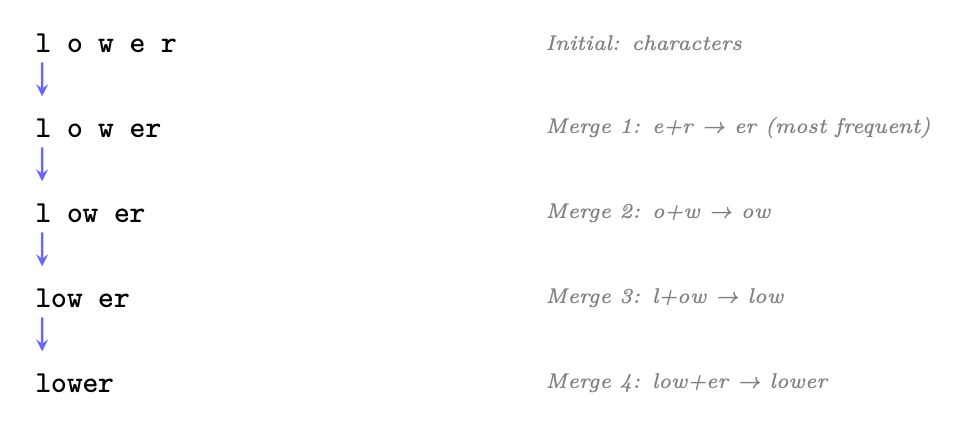
\includegraphics[width=0.65\textwidth]{figures/fig_003_fig3.png}
% \caption{BPE tokenization example: starting from characters, the algorithm iteratively merges the most frequent adjacent pairs until the word becomes a single token or the vocabulary budget is exhausted.}
\caption{BPE 分词示例：从字符开始，算法迭代地合并出现频率最高的相邻对，直到该词成为单个 Token 或词表预算耗尽。}
\end{figure}

\newpage
\subsection{其他分词方法}
\label{other-tokenization-methods}

\begin{table}[ht!]
\centering\small
% \caption{Comparison of subword tokenization algorithms.}
\caption{子词分词算法对比。}
\noindent\begin{tabularx}{\linewidth}{@{}l Z{0.88} Z{1.12}@{}}
\toprule
\textbf{方法} & \textbf{使用者} & \textbf{核心思想} \\
\midrule
BPE & GPT-4~\cite{openai2023gpt4}, Llama-3~\cite{grattafiori2024llama3}, Mistral~\cite{jiang2023mistral} & 自底向上合并频繁对；确定性 \\
WordPiece & BERT~\cite{devlin2019bert}, DistilBERT~\cite{sanh2019distilbert} & 类似 BPE，但最大化训练数据似然 \\
Unigram LM & SentencePiece & 自顶向下：从大词表开始，按似然影响剪枝 \\
字节级 BPE（Byte-level BPE） & GPT-2~\cite{radford2019gpt2}+ & 在原始字节上做 BPE（不可能出现未知 Token）；256 个基础词 \\
\bottomrule
\end{tabularx}
\end{table}

\subsection{分词最佳实践}
\label{tokenization-best-practices}

\begin{enumerate}
  % \item \textbf{Vocabulary size matters}: 32K is minimal; 128K enables better multilingual coverage and code handling. Llama-3 uses 128K tokens.
  \item \textbf{词表大小很重要}：32K 是最低限度；128K 能提供更好的多语种覆盖和代码处理能力。Llama-3 使用 128K Token。
  % \item \textbf{Special tokens}: Always include \texttt{<bos>}, \texttt{<eos>}, \texttt{<pad>}, \texttt{<unk>}. For instruction-tuned models, add role markers (\texttt{<|user|>}, \texttt{<|assistant|>}).
  \item \textbf{特殊 Token}：始终包含 \texttt{<bos>}、\texttt{<eos>}、\texttt{<pad>}、\texttt{<unk>}。对于指令微调模型，需添加角色标记（\texttt{<|user|>}、\texttt{<|assistant|>}）。
  % \item \textbf{Fertility}: Measure tokens-per-word across languages. High fertility (many tokens per word) indicates poor coverage for that language.
  \item \textbf{繁殖度（Fertility）}：度量各语种的每词 Token 数。高繁殖度（每词产生很多 Token）表示对该语种的覆盖较差。
  % \item \textbf{Never tokenize across boundaries}: Spaces, punctuation, and digits should be handled consistently. Most modern tokenizers prepend a space marker (``the'') to distinguish word-initial vs.~continuation tokens.
  \item \textbf{切勿跨边界分词}：空格、标点和数字应一致处理。大多数现代分词器会在前面添加空格标记（如 ``the''）以区分词首 Token 与词中续接 Token。
  % \item \textbf{Numbers}: Consider digit-level tokenization for arithmetic tasks. ``2024'' as [``2'',``0'',``2'',``4''] enables digit-by-digit reasoning.
  \item \textbf{数字}：对算术任务考虑数字级分词。``2024'' 切为 [``2'',``0'',``2'',``4''] 可以支持逐位推理。
  % \item \textbf{Code}: Ensure whitespace (indentation) is tokenized efficiently. Llama-3 tokenizes runs of spaces as single tokens.
  \item \textbf{代码}：确保高效地分词空白（缩进）。Llama-3 将连续空格分词为单个 Token。
\end{enumerate}

\subsection{分词实战：HuggingFace 示例}
\label{tokenization-in-practice-huggingface-example}

% The \texttt{transformers} library provides a unified interface for all tokenizers. The following demonstrates encoding and decoding with a modern LLM tokenizer:
\texttt{transformers} 库为所有分词器提供了统一接口。以下演示了使用现代 LLM 分词器进行编码和解码：

\begin{lstlisting}[style=pythonstyle, caption={使用 HuggingFace Transformers 进行分词的编码/解码。}]
from transformers import AutoTokenizer

# 加载 Llama-3 分词器（128K 词表，字节级 BPE）
tokenizer = AutoTokenizer.from_pretrained("meta-llama/Meta-Llama-3-8B")

text = "Reinforcement learning optimizes long-term rewards."

# 编码：文本 -> Token ID
token_ids = tokenizer.encode(text)
print(token_ids)
# [128000, 29934, 262, 11008, 4815, 6900, 1317, 9860, 21845, 13]

# 将单个 Token 解码以查看子词切分
tokens = tokenizer.convert_ids_to_tokens(token_ids)
print(tokens)
# ['<|begin_of_text|>', 'Re', 'inforce', 'ment', ' learning',
#  ' optimizes', ' long', '-term', ' rewards', '.']

# 解码回文本（双向往返）
reconstructed = tokenizer.decode(token_ids, skip_special_tokens=True)
assert reconstructed == text  # 完美重建

# 带注意力掩码的分词（用于带 padding 的批量输入）
batch = tokenizer(
    ["Short text.", "A much longer input sentence for comparison."],
    padding=True, return_tensors="pt"
)
print(batch.keys())  # dict_keys(['input_ids', 'attention_mask'])
\end{lstlisting}

\subsection{特殊 Token 与结构化提示}
\label{special-tokens-and-structured-prompts}

% Special tokens are reserved vocabulary entries that carry structural meaning rather than linguistic content. They are critical for controlling model behavior.
特殊 Token 是保留的词表条目，承载结构性含义而非语言内容。它们对控制模型行为至关重要。

\begin{table}[ht!]
\centering
% \caption{Common special tokens across LLM families.}
\caption{各类 LLM 中常见的特殊 Token。}
\begin{tabularx}{0.92\linewidth}{@{}Z{0.78} l Z{1.22}@{}}
\toprule
\textbf{Token} & \textbf{别名} & \textbf{用途} \\
\midrule
\texttt{<bos>} / \texttt{<|begin\_of\_text|>} & BOS & 标记序列开始 \\
\texttt{<eos>} / \texttt{<|end\_of\_text|>} & EOS & 标记序列结束；停止生成 \\
\texttt{<|user|>} & --- & 标记对话中用户轮次的开始 \\
\texttt{<|assistant|>} & --- & 标记对话中助手轮次的开始 \\
\texttt{<pad>} & PAD & 将批次填充到统一长度；在注意力中被掩盖 \\
\texttt{<unk>} & UNK & 词表外占位符（在 BPE 中很少出现） \\
\texttt{[SEP]} & SEP & 分隔片段（BERT 风格） \\
\texttt{[CLS]} & CLS & 分类 Token（BERT） \\
\texttt{[MASK]} & MASK & 用于掩码语言模型（MLM）预训练的掩码 Token \\
\bottomrule
\end{tabularx}
\end{table}

\paragraph{指令微调模型的角色标记。}
\label{role-markers-for-instruction-tuned-models.}

% Modern chat models use special tokens to delineate conversational structure. These are \textbf{not} trained to carry semantic meaning---they are structural delimiters that the model learns to parse:
现代对话模型使用特殊 Token 来界定对话结构。它们\textbf{并非}被训练来承载语义含义——而是结构分隔符，模型学习去解析它们：

\begin{lstlisting}[style=pythonstyle, caption={带特殊 Token 的对话模板（Llama-3 格式）。}]
# Llama-3 对话模板
messages = [
    {"role": "system", "content": "You are a helpful assistant."},
    {"role": "user", "content": "Explain PPO in one sentence."},
]

# apply_chat_template 处理所有特殊 Token 的插入
prompt = tokenizer.apply_chat_template(messages, tokenize=False)
print(prompt)
# <|begin_of_text|><|start_header_id|>system<|end_header_id|>
#
# You are a helpful assistant.<|eot_id|><|start_header_id|>user<|end_header_id|>
#
# Explain PPO in one sentence.<|eot_id|><|start_header_id|>assistant<|end_header_id|>
#
#
\end{lstlisting}

\begin{keybox}[特殊 Token 最佳实践]
\begin{itemize}
  % \item \textbf{Never split special tokens}: They must be atomic---ensure your tokenizer treats them as single units, not character sequences.
  \item \textbf{切勿拆分特殊 Token}：它们必须是原子单位——确保分词器将其视为单个单元，而非字符序列。
  % \item \textbf{Mask loss on special tokens}: During SFT, do not compute loss on structural tokens (role markers, separators). The model should not ``learn'' to predict formatting.
  \item \textbf{对特殊 Token 屏蔽损失}：在 SFT 期间，不要对结构性 Token（角色标记、分隔符）计算损失。模型不应``学习''预测格式本身。
  % \item \textbf{Use templates for structure}: Encode task semantics via special tokens rather than natural language instructions. E.g., \texttt{<|tool\_call|>} is more reliable than ``Now I will call a tool:''.
  \item \textbf{用模板表达结构}：通过特殊 Token 而非自然语言指令编码任务语义。例如，\texttt{<|tool\_call|>} 比 ``Now I will call a tool:'' 更可靠。
  % \item \textbf{Tool/function calling}: Define dedicated tokens like \texttt{<|function|>}, \texttt{<|result|>} to create unambiguous boundaries between reasoning and action.
  \item \textbf{工具/函数调用}：定义专用 Token，如 \texttt{<|function|>}、\texttt{<|result|>}，以在推理与动作之间建立无歧义的边界。
  % \item \textbf{Consistent handling in RL}: During PPO/GRPO, ensure the reference model and policy model use identical tokenization and special token handling---mismatches corrupt KL computation.
  \item \textbf{RL 中的一致处理}：在 PPO/GRPO 期间，确保参考模型与策略模型使用相同的分词和特殊 Token 处理——不一致会破坏 KL 计算。
  % \item \textbf{EOS handling}: During generation, ensure EOS is included in the action space. If the model cannot emit EOS, responses grow unbounded (common RL failure mode).
  \item \textbf{EOS 处理}：在生成时，确保 EOS 包含在动作空间中。若模型无法发出 EOS，回复将无界增长（常见的 RL 失败模式）。
\end{itemize}
\end{keybox}

\section{Transformer 架构}
\label{the-transformer-architecture}

% The Transformer~\cite{vaswani2017attention} is the foundation of all modern LLMs. Understanding its components is essential for grasping every optimization and training method in this guide.
Transformer~\cite{vaswani2017attention} 是所有现代 LLM 的基础。理解其组件对于把握本指南中的每种优化和训练方法都至关重要。

\subsection{整体结构}
\label{high-level-structure}

% A decoder-only transformer processes tokens sequentially through embedding, repeated attention+FFN blocks, and a final projection to vocabulary logits. Figure~\ref{fig:decoder-only} shows the complete architecture.
仅解码器（decoder-only）的 Transformer 依次通过嵌入层、重复的注意力+FFN 块以及最终对词表 logits 的投影来处理 Token。图~\ref{fig:decoder-only} 展示了完整架构。

\begin{figure}[ht!]
\centering
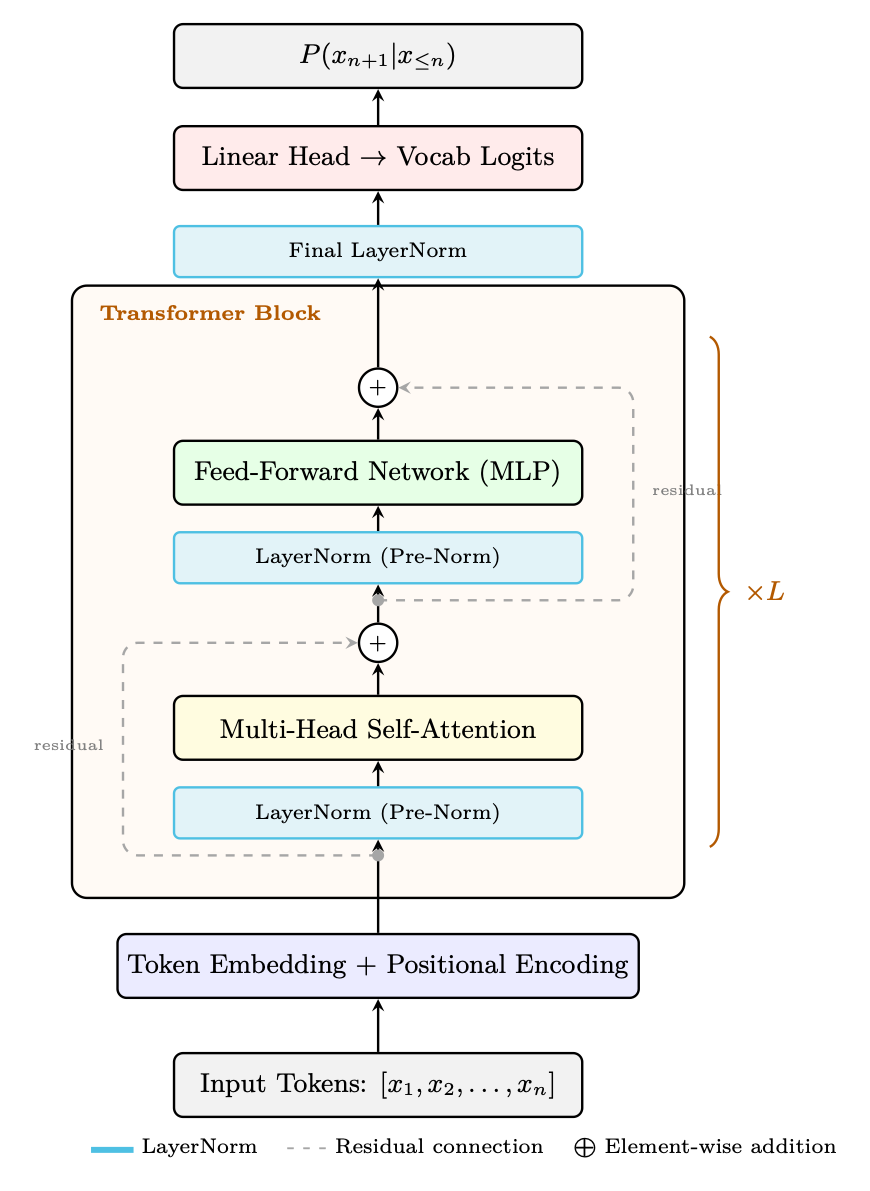
\includegraphics[width=0.55\textwidth]{figures/fig_004_decoder-only.png}
% \caption{Decoder-only Transformer block (GPT-style, Pre-Norm variant). Each sub-layer (attention, FFN) is preceded by LayerNorm and followed by a residual addition: $\mathbf{x} + \text{SubLayer}(\text{LN}(\mathbf{x}))$. This Pre-Norm ordering (used by Llama, GPT-3, Mistral) stabilizes training without warmup, unlike the original Post-Norm (which applies LayerNorm after the addition). $L$ identical blocks are stacked, followed by a final LayerNorm and linear projection to vocabulary logits.}
\caption{仅解码器 Transformer 块（GPT 风格，Pre-Norm 变体）。每个子层（注意力、FFN）之前先经过 LayerNorm，之后接残差相加：$\mathbf{x} + \text{SubLayer}(\text{LN}(\mathbf{x}))$。这种 Pre-Norm 顺序（被 Llama、GPT-3、Mistral 采用）在无需 warmup 的情况下稳定训练，不同于原始的 Post-Norm（在相加之后应用 LayerNorm）。$L$ 个相同的块被堆叠，之后是一个最终的 LayerNorm 和到词表 logits 的线性投影。}
\label{fig:decoder-only}
\end{figure}

\subsection{原始的编码器-解码器 Transformer}
\label{the-original-encoder-decoder-transformer}

% The Transformer was originally introduced~\cite{vaswani2017attention} as an \textbf{encoder-decoder} architecture for sequence-to-sequence tasks (machine translation, summarization). While modern LLMs predominantly use decoder-only variants (GPT-style), understanding the full architecture is essential because cross-attention and masked self-attention --- both originating here --- remain fundamental building blocks.
Transformer 最初被提出~\cite{vaswani2017attention} 时是一种用于序列到序列任务（机器翻译、摘要）的\textbf{编码器-解码器}架构。尽管现代 LLM 主要使用仅解码器变体（GPT 风格），理解完整架构仍然至关重要，因为交叉注意力和带掩码的自注意力——两者都起源于此——仍是基础构建模块。

\begin{figure}[ht!]
\centering
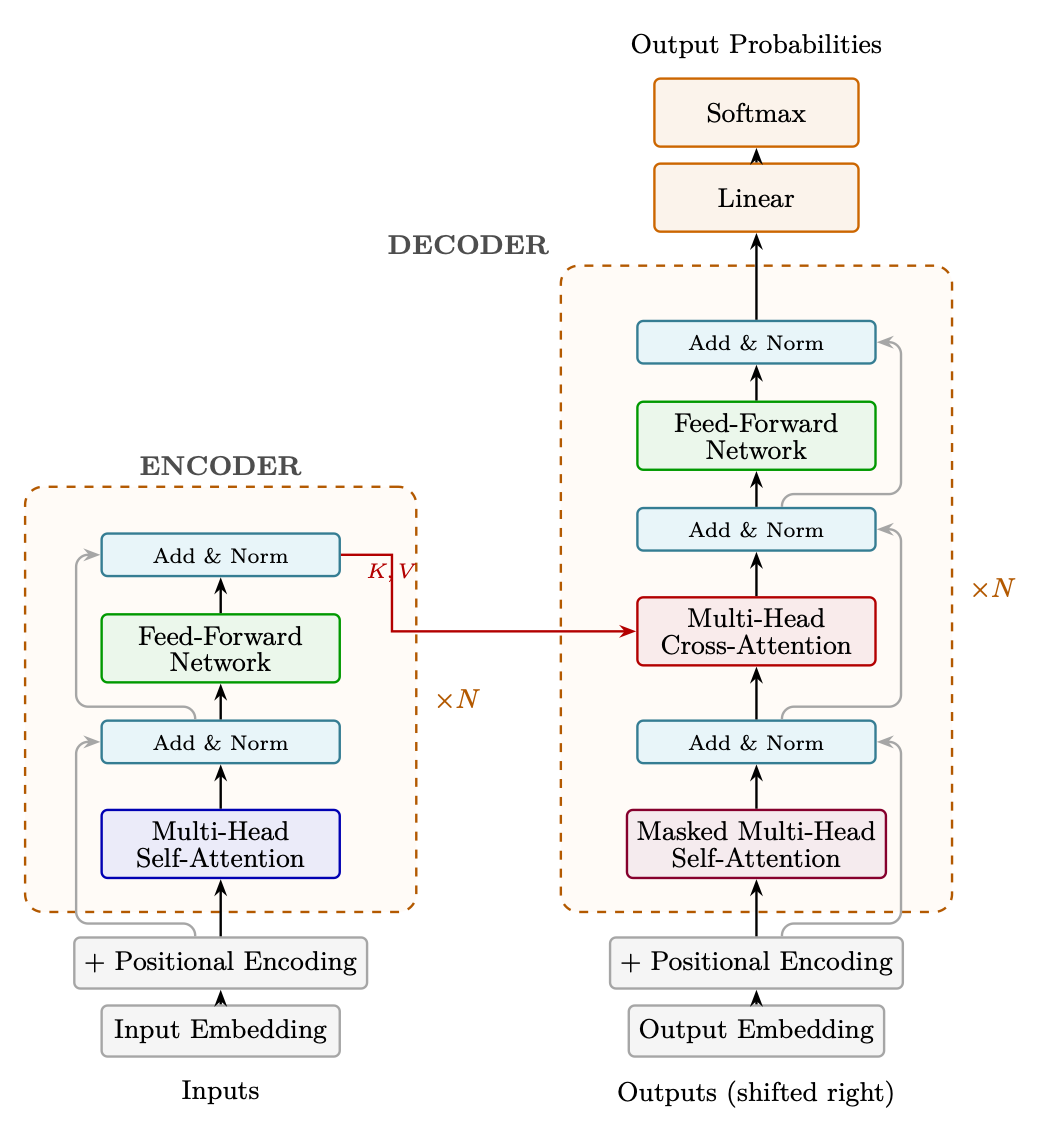
\includegraphics[width=0.85\textwidth]{figures/fig_005_transformer-original.png}
% \caption{The original Transformer architecture (Vaswani et al., 2017). The encoder (left) processes the full input with bidirectional self-attention. The decoder (right) generates tokens autoregressively using masked self-attention and cross-attention to encoder representations. Dashed boxes indicate the repeated layer block ($\times N$); gray lines show residual connections bypassing each sub-layer. Note: the original work uses \textbf{Post-Norm} (LayerNorm applied \emph{after} the residual addition: $\text{LN}(\mathbf{x} + \text{SubLayer}(\mathbf{x}))$), unlike modern LLMs which use Pre-Norm.}
\caption{原始 Transformer 架构（Vaswani 等，2017）。编码器（左）通过双向自注意力处理整个输入。解码器（右）使用带掩码的自注意力以及对编码器表征的交叉注意力来自回归生成 Token。虚线框表示重复的层块（$\times N$）；灰线表示绕过每个子层的残差连接。注意：原始工作使用 \textbf{Post-Norm}（LayerNorm 在残差相加\emph{之后}应用：$\text{LN}(\mathbf{x} + \text{SubLayer}(\mathbf{x}))$），不同于现代 LLM 使用 Pre-Norm。}
\label{fig:transformer-original}
\end{figure}

\paragraph{编码器（Encoder）。}
\label{encoder.}

% The encoder processes the entire input sequence \emph{bidirectionally} --- each token attends to all other tokens (no causal mask). This produces a rich contextual representation $\mathbf{H}^{\text{enc}} \in \mathbb{R}^{n \times d}$ where each position encodes information about the full input:
编码器\emph{双向}地处理整个输入序列——每个 Token 关注所有其他 Token（无因果掩码）。这产生了丰富的上下文表征 $\mathbf{H}^{\text{enc}} \in \mathbb{R}^{n \times d}$，其中每个位置都编码了关于整个输入的信息：

\begin{itemize}
  % \item \textbf{Input}: Token embeddings + sinusoidal positional encodings
  \item \textbf{输入}：Token 嵌入 + 正弦位置编码
  % \item \textbf{Each layer}: Multi-Head Self-Attention $\to$ Add \& Norm $\to$ FFN $\to$ Add \& Norm
  \item \textbf{每一层}：多头自注意力 $\to$ Add \& Norm $\to$ FFN $\to$ Add \& Norm
  % \item \textbf{No causal mask}: Position $i$ attends to all positions $1, \ldots, n$
  \item \textbf{无因果掩码}：位置 $i$ 关注所有位置 $1, \ldots, n$
  % \item \textbf{Output}: Contextual representations of the full input sequence
  \item \textbf{输出}：整个输入序列的上下文表征
\end{itemize}

\paragraph{解码器——带掩码的多头自注意力。}
\label{decoder-masked-multi-head-self-attention.}

% The decoder generates output tokens one at a time (autoregressively). To prevent the model from ``seeing the future,'' the self-attention in the decoder uses a \textbf{causal mask}:
解码器一次生成一个输出 Token（自回归地）。为了防止模型``看到未来''，解码器中的自注意力使用\textbf{因果掩码（causal mask）}：

\begin{equation}
  \text{MaskedAttn}(Q, K, V) = \text{softmax}\!\left(\frac{QK^T}{\sqrt{d_k}} + M\right) V
\end{equation}

% where the mask $M$ is:
其中掩码 $M$ 为：
\[
M_{ij} = \begin{cases} 0 & \text{if } i \geq j \text{ (can attend)} \\ -\infty & \text{if } i < j \text{ (future token --- blocked)} \end{cases}
\]

\begin{intuitionbox}[为什么掩码很重要]
% During training, the decoder processes the entire target sequence in parallel (teacher forcing), but each position must only attend to previous positions to maintain the autoregressive property. The mask ensures that generating token $t$ uses only information from tokens $1, \ldots, t{-}1$. At inference, tokens are generated one-by-one so the mask is implicit --- but during training it enables parallel computation while preserving causality.
在训练期间，解码器并行处理整个目标序列（teacher forcing），但每个位置只能关注之前的位置以保持自回归特性。掩码确保生成 Token $t$ 时仅使用 Token $1, \ldots, t{-}1$ 的信息。在推理时，Token 是逐一生成的，因此掩码是隐式的——但在训练期间，它使并行计算成为可能，同时保持因果性。
\end{intuitionbox}

\paragraph{解码器——交叉注意力。}
\label{decoder-cross-attention.}

% After masked self-attention, each decoder layer applies \textbf{cross-attention} where the decoder attends to the encoder's output representations. This is the mechanism by which the decoder ``reads'' the input:
在带掩码的自注意力之后，每个解码器层应用\textbf{交叉注意力（cross-attention）}，解码器关注编码器的输出表征。这是解码器``读取''输入的机制：

\begin{equation}
  \text{CrossAttn}(Q_{\text{dec}}, K_{\text{enc}}, V_{\text{enc}}) = \text{softmax}\!\left(\frac{Q_{\text{dec}} K_{\text{enc}}^T}{\sqrt{d_k}}\right) V_{\text{enc}}
\end{equation}

\begin{itemize}
  % \item \textbf{Queries} come from the decoder's previous sublayer (the masked self-attention output)
  \item \textbf{Query} 来自解码器之前的子层（带掩码自注意力的输出）
  % \item \textbf{Keys and Values} come from the encoder's final output $\mathbf{H}^{\text{enc}}$
  \item \textbf{Key 和 Value} 来自编码器的最终输出 $\mathbf{H}^{\text{enc}}$
  % \item \textbf{No mask} is applied --- every decoder position can attend to every encoder position
  \item \textbf{不应用掩码}——每个解码器位置可以关注每个编码器位置
  % \item This allows the decoder to dynamically focus on different parts of the input at each generation step (e.g., attending to ``cat'' when translating to ``gato'' in English$\to$Spanish)
  \item 这使得解码器在每个生成步骤可以动态聚焦于输入的不同部分（例如，在英语$\to$西班牙语翻译中，生成 ``gato'' 时关注 ``cat''）
\end{itemize}

\paragraph{完整的解码器层。}
\label{full-decoder-layer.}

% Each decoder layer contains three sublayers (vs.~two in the encoder):
每个解码器层包含三个子层（编码器只有两个）：

\begin{enumerate}
  % \item \textbf{Masked Multi-Head Self-Attention} + Residual + LayerNorm
  \item \textbf{带掩码的多头自注意力} + 残差 + LayerNorm
  % \item \textbf{Multi-Head Cross-Attention} (to encoder output) + Residual + LayerNorm
  \item \textbf{多头交叉注意力}（对编码器输出）+ 残差 + LayerNorm
  % \item \textbf{Feed-Forward Network} + Residual + LayerNorm
  \item \textbf{前馈网络（Feed-Forward Network）} + 残差 + LayerNorm
\end{enumerate}

\paragraph{从编码器-解码器到仅解码器。}
\label{from-encoder-decoder-to-decoder-only.}

% Modern LLMs (GPT, Llama, Qwen) use only the decoder, removing both the encoder and cross-attention layers entirely. The key insight: for generative language modeling, a single causal (masked) self-attention stack is sufficient --- the model learns to encode context and generate continuations in a single pass. This simplifies architecture, training, and inference while scaling more effectively. Encoder-decoder models (T5, BART) remain relevant for tasks with distinct input/output structure (translation, summarization), and cross-attention reappears in multimodal models where vision encoders provide keys/values to language decoders.
现代 LLM（GPT、Llama、Qwen）只使用解码器，完全移除了编码器和交叉注意力层。关键洞察：对于生成式语言建模，单个因果（掩码）自注意力栈就足够了——模型在单次传递中学会编码上下文并生成后续内容。这简化了架构、训练和推理，并且更有效地扩展规模。编码器-解码器模型（T5、BART）对于具有明确输入/输出结构的任务（翻译、摘要）仍然有意义，而交叉注意力在多模态模型中再次出现，其中视觉编码器为语言解码器提供 Key/Value。

\subsection{仅解码器 vs 编码器-解码器}
\label{decoder-only-vs-encoder-decoder}

% Modern LLMs almost exclusively use decoder-only architectures, but understanding the trade-offs with encoder-decoder designs clarifies why.
现代 LLM 几乎只使用仅解码器架构，但理解与编码器-解码器设计的权衡有助于阐明原因。

\noindent\begin{tabularx}{\linewidth}{@{}l Z{1.42} Z{0.58}@{}}
\toprule
\textbf{架构} & \textbf{示例} & \textbf{使用场景} \\
\midrule
仅解码器 & GPT-4~\cite{openai2023gpt4}, Llama~\cite{grattafiori2024llama3}, Mistral~\cite{jiang2023mistral}, Qwen~\cite{qwen2024qwen25} & 自回归生成；在对话/推理领域占主导 \\
编码器-解码器 & T5~\cite{raffel2020t5}, BART~\cite{lewis2020bart}, Flan-T5~\cite{chung2022flan} & Seq2seq（翻译、摘要）；现在较少使用 \\
仅编码器 & BERT~\cite{devlin2019bert}, RoBERTa~\cite{liu2019roberta} & 分类/嵌入；不用于生成 \\
\bottomrule
\end{tabularx}

\begin{warningbox}[为什么仅解码器胜出]
% Decoder-only models are simpler (one model, one loss), scale better (all parameters contribute to generation), and support unified training (pretraining = next-token prediction = fine-tuning objective). Encoder-decoder models waste capacity on the encoder for pure generation tasks.
仅解码器模型更简单（单一模型，单一损失），扩展性更好（所有参数都参与生成），并且支持统一的训练（预训练 = 下一个 Token 预测 = 微调目标）。对于纯生成任务，编码器-解码器模型在编码器上浪费了容量。
\end{warningbox}

\subsection{嵌入：从离散 Token 到连续空间}
\label{embeddings-from-discrete-tokens-to-continuous-space}

% Before any attention or computation happens, the transformer must convert discrete token IDs into continuous vectors that neural networks can process. This is the role of the \textbf{embedding layer}.
在任何注意力或计算发生之前，Transformer 必须将离散的 Token ID 转换为神经网络可处理的连续向量。这就是\textbf{嵌入层（embedding layer）}的作用。

\paragraph{什么是嵌入？}
\label{what-is-an-embedding}

% An embedding is a learned dense vector representation of a discrete symbol. Instead of representing the word ``king'' as a one-hot vector of size $|\mathcal{V}| = 128{,}000$ (mostly zeros), we represent it as a compact vector in $\mathbb{R}^d$ (e.g., $d = 4096$) that captures its \emph{meaning}.
嵌入是一个离散符号的学习得到的稠密向量表示。我们不再把单词 ``king'' 表示为大小为 $|\mathcal{V}| = 128{,}000$ 的独热向量（大部分为零），而是表示为 $\mathbb{R}^d$（例如 $d = 4096$）中一个紧凑的向量，捕捉其\emph{含义}。

% The key insight: \textbf{similar concepts get nearby vectors}. In a well-trained embedding space:
关键洞察：\textbf{相似的概念得到相近的向量}。在一个训练良好的嵌入空间中：

\begin{itemize}
  % \item ``king'' and ``queen'' are close (both royalty)
  \item ``king'' 和 ``queen'' 接近（都是王室）
  % \item ``king'' and ``bicycle'' are far apart (unrelated)
  \item ``king'' 和 ``bicycle'' 距离很远（无关）
  % \item Vector arithmetic captures relationships: $\vec{\text{king}} - \vec{\text{man}} + \vec{\text{woman}} \approx \vec{\text{queen}}$
  \item 向量运算捕捉关系：$\vec{\text{king}} - \vec{\text{man}} + \vec{\text{woman}} \approx \vec{\text{queen}}$
\end{itemize}

\begin{figure}[ht!]
\centering
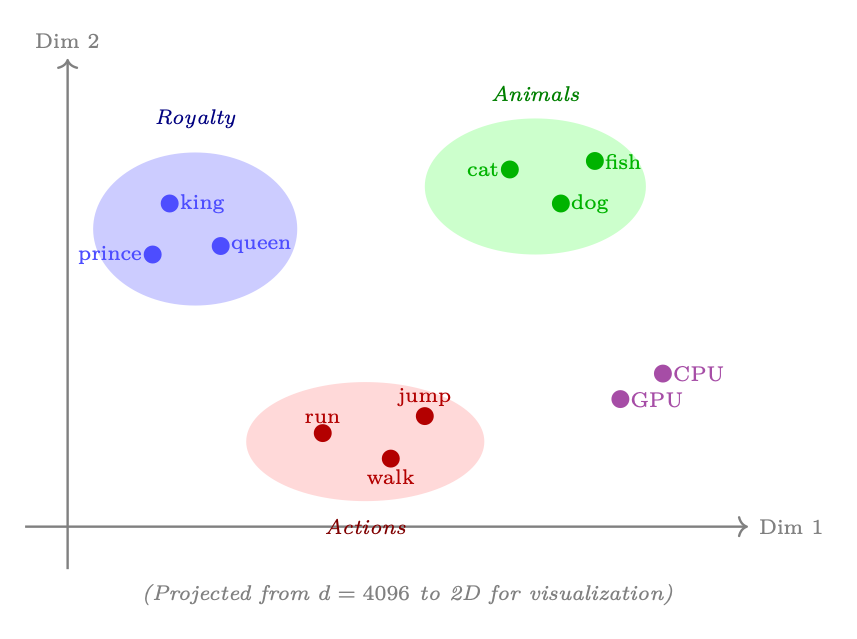
\includegraphics[width=0.85\textwidth]{figures/fig_006_fig6.png}
% \caption{Embedding space visualization (2D projection): semantically similar words cluster together. The embedding table learns these positions during pretraining, capturing meaning purely from co-occurrence patterns in text.}
\caption{嵌入空间可视化（二维投影）：语义相似的词聚集在一起。嵌入表在预训练期间学习这些位置，纯粹从文本中的共现模式中捕捉含义。}
\end{figure}

\paragraph{嵌入表。}
\label{the-embedding-table.}

% In practice, the embedding layer is simply a matrix $\mathbf{E} \in \mathbb{R}^{|\mathcal{V}| \times d}$ where row $i$ stores the embedding vector for token $i$:
在实践中，嵌入层就是一个矩阵 $\mathbf{E} \in \mathbb{R}^{|\mathcal{V}| \times d}$，其中第 $i$ 行存储 Token $i$ 的嵌入向量：

\begin{equation}
\text{embed}(x_t) = \mathbf{E}[x_t] \in \mathbb{R}^d
\end{equation}

% For a sequence of token IDs $[x_1, x_2, \ldots, x_n]$, embedding is a simple table lookup (indexing operation):
对于一个 Token ID 序列 $[x_1, x_2, \ldots, x_n]$，嵌入只是一个简单的表查询（索引操作）：
\[
\mathbf{H}_0 = [\mathbf{E}[x_1];\; \mathbf{E}[x_2];\; \ldots;\; \mathbf{E}[x_n]] \in \mathbb{R}^{n \times d}
\]

\begin{keybox}[Transformer 中的嵌入表]
\begin{itemize}
  % \item \textbf{Size}: $|\mathcal{V}| \times d$. For Llama-3: $128{,}256 \times 4{,}096 = 525$M parameters (6.5\% of 8B model).
  \item \textbf{尺寸}：$|\mathcal{V}| \times d$。对于 Llama-3：$128{,}256 \times 4{,}096 = 525$M 参数（占 8B 模型的 6.5\%）。
  % \item \textbf{Initialization}: Random (Xavier/normal), then learned via backpropagation.
  \item \textbf{初始化}：随机（Xavier/正态分布），然后通过反向传播学习。
  % \item \textbf{Weight tying}: Many models \emph{share} the embedding matrix with the output projection head: $W_{\text{head}} = \mathbf{E}^T$. This saves parameters and creates a symmetric encode-decode structure.
  \item \textbf{权重共享（Weight tying）}：许多模型\emph{共享}嵌入矩阵与输出投影头：$W_{\text{head}} = \mathbf{E}^T$。这节省参数并创建对称的编码-解码结构。
  % \item \textbf{Input}: Token ID (integer) $\to$ \textbf{Output}: Dense vector in $\mathbb{R}^d$.
  \item \textbf{输入}：Token ID（整数）$\to$ \textbf{输出}：$\mathbb{R}^d$ 中的稠密向量。
  % \item \textbf{Gradient flow}: During training, only the rows corresponding to tokens in the current batch receive gradient updates (sparse update).
  \item \textbf{梯度流}：在训练期间，只有当前批次中 Token 对应的行接收梯度更新（稀疏更新）。
\end{itemize}
\end{keybox}

\begin{intuitionbox}[为什么嵌入有效]
% The embedding table is learned end-to-end with the rest of the model. Because the model is trained to predict the next token, it must learn representations where tokens that appear in similar contexts get similar vectors. This is the distributional hypothesis: ``you shall know a word by the company it keeps''~\cite{firth1957synopsis}. The embedding layer compresses this statistical structure into dense geometry.
嵌入表与模型其余部分端到端地一起学习。因为模型被训练去预测下一个 Token，它必须学到这样的表征：出现在相似上下文中的 Token 得到相似的向量。这就是分布假说：``你应当通过一个词的伙伴来了解它''~\cite{firth1957synopsis}。嵌入层将这种统计结构压缩为稠密几何。
\end{intuitionbox}

\paragraph{各向异性（anisotropy）问题。}
\label{the-anisotropy-problem.}

% A critical issue arises when using pretrained embeddings (e.g., from BERT or GPT-2) for downstream tasks like retrieval (RAG) or bootstrapping recommender systems: the learned representations are highly \textbf{anisotropic}---they occupy a narrow cone in the embedding space rather than being uniformly distributed across all directions~\cite{ethayarajh2019contextual}.
当使用预训练嵌入（例如来自 BERT 或 GPT-2）用于下游任务（如检索 RAG 或推荐系统冷启动）时，会出现一个关键问题：学习到的表征高度\textbf{各向异性（anisotropic）}——它们占据嵌入空间中一个狭窄的锥形区域，而非均匀分布在所有方向上~\cite{ethayarajh2019contextual}。

\begin{figure}[ht!]
\centering
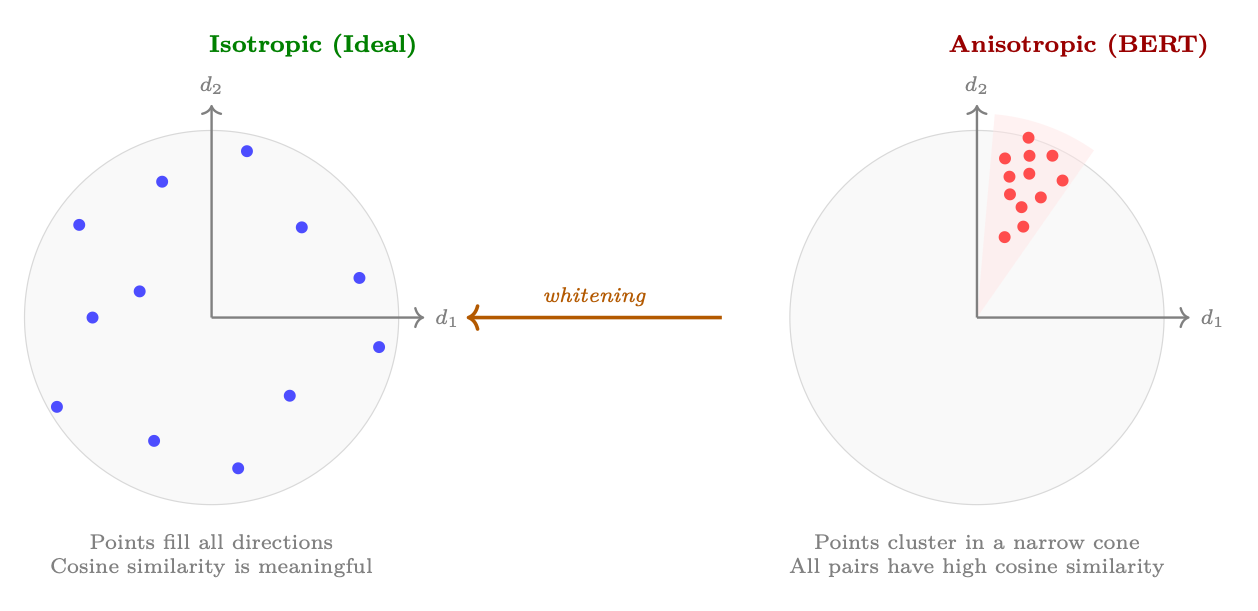
\includegraphics[width=0.85\textwidth]{figures/fig_007_fig7.png}
% \caption{Isotropy vs. anisotropy in embedding spaces. Left: isotropic embeddings spread uniformly, making cosine similarity a reliable measure of semantic relatedness. Right: anisotropic embeddings (as found in BERT) cluster in a narrow cone, causing all pairs to have high cosine similarity regardless of semantic content. Whitening transforms the space to restore isotropy.}
\caption{嵌入空间中的各向同性（isotropy）与各向异性（anisotropy）。左：各向同性的嵌入均匀分布，使余弦相似度成为可靠的语义相关性度量。右：各向异性的嵌入（如 BERT 中观察到的）聚集在狭窄的锥形内，导致所有对的余弦相似度都很高，无论语义内容如何。白化（whitening）变换空间以恢复各向同性。}
\end{figure}

\textbf{这为何对应用很重要：}

\begin{itemize}
  % \item \textbf{RAG / Retrieval}: If all embeddings have cosine similarity $>0.7$ regardless of content, retrieval rankings become nearly random---the system cannot distinguish relevant from irrelevant passages.
  \item \textbf{RAG / 检索}：如果所有嵌入无论内容如何余弦相似度都 $>0.7$，检索排名几乎成为随机——系统无法区分相关与不相关的段落。
  % \item \textbf{Recommender systems}: Using pretrained LLM embeddings to represent items/users only works if the geometry preserves meaningful similarity structure.
  \item \textbf{推荐系统}：使用预训练 LLM 嵌入来表示物品/用户，只有在几何结构保留了有意义的相似性结构时才有效。
  % \item \textbf{Clustering}: Anisotropic embeddings collapse clusters, making it impossible to discover natural groupings.
  \item \textbf{聚类}：各向异性的嵌入使聚类塌缩，无法发现自然分组。
\end{itemize}

\paragraph{解决方案：白化（whitening）。}
\label{resolution-whitening.}

% A simple and effective fix is \textbf{whitening}~\cite{su2021whitening}---a linear transformation that makes the embedding distribution isotropic (zero mean, identity covariance):
一个简单有效的解决方法是\textbf{白化（whitening）}~\cite{su2021whitening}——一种使嵌入分布变得各向同性（零均值、单位协方差）的线性变换：

\begin{equation}
\tilde{\mathbf{h}} = \mathbf{D}^{-1/2} \mathbf{U}^T (\mathbf{h} - \boldsymbol{\mu})
\end{equation}

% where $\boldsymbol{\mu}$ is the mean embedding, and $\mathbf{U}\mathbf{D}\mathbf{U}^T$ is the eigendecomposition of the covariance matrix $\Sigma = \frac{1}{N}\sum_i (\mathbf{h}_i - \boldsymbol{\mu})(\mathbf{h}_i - \boldsymbol{\mu})^T$.
其中 $\boldsymbol{\mu}$ 是平均嵌入，$\mathbf{U}\mathbf{D}\mathbf{U}^T$ 是协方差矩阵 $\Sigma = \frac{1}{N}\sum_i (\mathbf{h}_i - \boldsymbol{\mu})(\mathbf{h}_i - \boldsymbol{\mu})^T$ 的特征分解。

\begin{keybox}[白化的实践]
\begin{itemize}
  % \item \textbf{What it does}: Rotates and scales the embedding space so all directions have equal variance (unit covariance).
  \item \textbf{作用}：旋转并缩放嵌入空间，使所有方向具有相等的方差（单位协方差）。
  % \item \textbf{Effect}: Cosine similarity becomes meaningful---semantically similar pairs score high, dissimilar pairs score low.
  \item \textbf{效果}：余弦相似度变得有意义——语义相似的对得分高，不相似的对得分低。
  % \item \textbf{Bonus}: Can simultaneously reduce dimensionality by keeping only the top-$k$ eigenvectors (similar to PCA), making retrieval faster.
  \item \textbf{额外好处}：可以同时通过仅保留前 $k$ 个特征向量来降维（类似 PCA），使检索更快。
  % \item \textbf{Cost}: Requires computing the covariance matrix over a representative corpus (one-time, $O(N \cdot d^2)$). The transform itself is a simple matrix multiply at inference.
  \item \textbf{成本}：需要在一个代表性语料上计算协方差矩阵（一次性，$O(N \cdot d^2)$）。变换本身在推理时只是简单的矩阵乘法。
  % \item \textbf{Alternative approaches}: Contrastive fine-tuning (SimCSE), flow-based normalization, or training with isotropy-promoting regularizers.
  \item \textbf{替代方法}：对比微调（SimCSE）、基于 flow 的归一化，或使用促进各向同性的正则项进行训练。
\end{itemize}
\end{keybox}

\subsection{自注意力机制}
\label{self-attention-mechanism}

% Self-attention is the core operation that allows each token to attend to every other token in the sequence, computing a weighted combination based on relevance.
自注意力是核心操作，它允许每个 Token 关注序列中的每一个其他 Token，基于相关性计算加权组合。

\begin{keybox}[缩放点积注意力（Scaled Dot-Product Attention）]
% Given input sequence $X \in \mathbb{R}^{n \times d}$, we compute:
给定输入序列 $X \in \mathbb{R}^{n \times d}$，我们计算：
\[
Q = XW_Q, \quad K = XW_K, \quad V = XW_V \quad (W_Q, W_K, W_V \in \mathbb{R}^{d \times d_k})
\]

\[
\text{Attention}(Q, K, V) = \text{softmax}\!\left(\frac{QK^T}{\sqrt{d_k}} + M\right) V
\]
% where $M$ is the \textbf{causal mask} (for autoregressive models): $M_{ij} = 0$ if $i \geq j$, else $-\infty$.
其中 $M$ 是\textbf{因果掩码}（用于自回归模型）：若 $i \geq j$ 则 $M_{ij} = 0$，否则为 $-\infty$。

% \textbf{Intuition}: Each token ``attends'' to all previous tokens, computing a weighted average of their values based on query-key similarity.
\textbf{直觉}：每个 Token``关注''所有先前的 Token，基于 query-key 相似度计算其 value 的加权平均。
\end{keybox}

\paragraph{计算复杂度。}
\label{computational-complexity.}

% The naive attention computation has \textbf{quadratic cost} in sequence length:
朴素的注意力计算在序列长度上具有\textbf{平方代价}：

\begin{itemize}
  % \item \textbf{Time}: $O(n^2 \cdot d)$ --- computing $QK^T$ requires $n^2$ dot products, each of dimension $d_k$.
  \item \textbf{时间}：$O(n^2 \cdot d)$——计算 $QK^T$ 需要 $n^2$ 个点积，每个维度为 $d_k$。
  % \item \textbf{Memory}: $O(n^2)$ --- the full attention matrix must be materialized to apply softmax.
  \item \textbf{内存}：$O(n^2)$——必须物化完整的注意力矩阵才能应用 Softmax。
\end{itemize}

% For a 128K-token context with $d = 4096$, the attention matrix alone is $128\text{K} \times 128\text{K} = 16.4$ billion entries (64 GB in FP32). This quadratic scaling is the fundamental bottleneck for long-context LLMs.
对于一个 $d = 4096$ 的 128K Token 上下文，仅注意力矩阵就是 $128\text{K} \times 128\text{K} = 164$ 亿个元素（FP32 下为 64 GB）。这种平方扩展是长上下文 LLM 的根本瓶颈。

\vspace{6pt}
\begin{table}[ht!]
\centering
% \caption{Attention cost scaling: why naive implementation is prohibitive for long sequences.}
\caption{注意力代价的扩展：为何朴素实现对长序列不可行。}
\begin{tabular}{@{}llll@{}}
\toprule
\textbf{序列长度} & \textbf{注意力操作数} & \textbf{矩阵大小} & \textbf{实际影响} \\
\midrule
2K & 4M & 16 MB & 快速；可放入 SRAM \\
8K & 64M & 256 MB & 用 FlashAttention 可应对 \\
32K & 1B & 4 GB & 需要内存高效内核 \\
128K & 16B & 64 GB & 超出单块 GPU 的 HBM \\
1M & 1T & 4 TB & 不使用次平方方法则不可行 \\
\bottomrule
\end{tabular}
\end{table}

\paragraph{驯服注意力代价的方法。}
\label{approaches-to-taming-attention-cost.}

% Several families of solutions address this quadratic bottleneck:
有几类方案可以应对这种平方瓶颈：

\begin{enumerate}
  % \item \textbf{Exact attention with IO-awareness (FlashAttention~\cite{dao2022flashattention})}: Does not reduce computational complexity but eliminates the need to materialize the $n \times n$ matrix in HBM by computing attention in tiles that fit in SRAM. Crucially, FlashAttention is \textbf{orthogonal} to the sparse patterns below---it is an execution engine, not an attention pattern. Production systems routinely combine FlashAttention with sliding windows or block-sparse masks, getting both IO efficiency and reduced FLOPs. We cover the algorithm in detail in Section~\ref{flash-attention-algorithm-and-hardware-awareness}.
  \item \textbf{具备 IO 感知的精确注意力（FlashAttention~\cite{dao2022flashattention}）}：不降低计算复杂度，但通过将注意力计算分块到能放入 SRAM 的瓦片中，消除了在 HBM 中物化 $n \times n$ 矩阵的需要。关键的是，FlashAttention 与下面的稀疏模式\textbf{正交}——它是一种执行引擎，而非注意力模式。生产系统通常将 FlashAttention 与滑动窗口或块稀疏掩码结合使用，同时获得 IO 效率和 FLOPs 减少。我们在第~\ref{flash-attention-algorithm-and-hardware-awareness} 节详细介绍该算法。
  % \item \textbf{Sliding window / local attention}: Each token only attends to the $w$ nearest tokens (e.g., $w = 4096$). Cost becomes $O(n \cdot w)$---linear in $n$. Used by Mistral~\cite{jiang2023mistral} (window $= 4096$) and Longformer~\cite{beltagy2020longformer}. Trades global context for efficiency; works well because most attention is local in practice. In modern stacks, the sliding-window mask is executed \emph{inside} a FlashAttention kernel.
  \item \textbf{滑动窗口 / 局部注意力}：每个 Token 只关注最近的 $w$ 个 Token（例如 $w = 4096$）。代价变为 $O(n \cdot w)$——在 $n$ 上是线性的。被 Mistral~\cite{jiang2023mistral}（窗口 $= 4096$）和 Longformer~\cite{beltagy2020longformer} 采用。以全局上下文换效率；之所以有效，是因为实践中大部分注意力是局部的。在现代技术栈中，滑动窗口掩码在 FlashAttention 内核\emph{内部}执行。
  % \item \textbf{Sparse attention patterns}: Combine local windows with periodic global tokens (e.g., every 512th token attends to all). BigBird~\cite{zaheer2020bigbird} and LongT5~\cite{guo2022longt5} use this. Preserves some long-range connectivity at $O(n\sqrt{n})$ cost. Again, FlashAttention serves as the underlying kernel for the non-zero attention blocks.
  \item \textbf{稀疏注意力模式}：将局部窗口与周期性的全局 Token 结合（例如，每隔 512 个 Token 关注全部）。BigBird~\cite{zaheer2020bigbird} 和 LongT5~\cite{guo2022longt5} 使用此方法。以 $O(n\sqrt{n})$ 代价保留一些长程连通性。同样，FlashAttention 作为非零注意力块的底层内核。
  % \item \textbf{Linear attention / state-space models}: Replace $\text{softmax}(QK^T)V$ with $\phi(Q)(\phi(K)^T V)$ using associativity, or reformulate as a recurrence (Mamba~\cite{gu2023mamba}, RWKV~\cite{peng2023rwkv}). Theoretically $O(n \cdot d^2)$ total. Unlike approaches 2--3 above, these are \emph{architectural replacements} that alter model expressiveness---softmax-free attention is fundamentally less expressive, and empirically these models still lag behind transformers on tasks requiring precise long-range retrieval or complex reasoning.
  \item \textbf{线性注意力 / 状态空间模型}：利用结合律将 $\text{softmax}(QK^T)V$ 替换为 $\phi(Q)(\phi(K)^T V)$，或重构为递归形式（Mamba~\cite{gu2023mamba}、RWKV~\cite{peng2023rwkv}）。理论上总代价为 $O(n \cdot d^2)$。与上面方法 2--3 不同，这些是\emph{架构上的替换}，改变了模型的表达能力——无 Softmax 的注意力本质上表达力更弱，经验上这些模型在需要精确长程检索或复杂推理的任务上仍然落后于 Transformer。
  % \item \textbf{KV cache compression}: At inference, compress or evict old KV pairs to bound memory. Techniques include: H$_2$O~\cite{zhang2023h2o} (heavy-hitter oracle---keep only high-attention keys), StreamingLLM~\cite{xiao2024streamingllm} (keep initial ``attention sink'' tokens + recent window), and quantized KV caches~\cite{liu2024kivi}.
  \item \textbf{KV 缓存压缩}：在推理时，压缩或驱逐旧的 KV 对以限制内存。技术包括：H$_2$O~\cite{zhang2023h2o}（重击者预言机——只保留高注意力的 Key）、StreamingLLM~\cite{xiao2024streamingllm}（保留初始``注意力陷阱（Attention Sink）''Token + 最近窗口），以及量化 KV 缓存~\cite{liu2024kivi}。
\end{enumerate}

\begin{intuitionbox}[FlashAttention + 稀疏模式 = 两全其美]
% A common misconception is that FlashAttention is an \emph{alternative} to sparse attention. It is not---it is an IO optimization for the attention kernel that composes freely with any attention mask. Modern production systems (e.g., Mistral, DeepSeek) use FlashAttention as the execution engine \emph{underneath} a sliding-window or block-sparse mask. This gives you both reduced FLOPs (from sparsity) and optimal memory access patterns (from tiling). RingAttention~\cite{liu2023ringattention} extends this further to multi-device settings, distributing the tiled computation across GPUs along the sequence dimension.
一个常见误解是 FlashAttention 是稀疏注意力的\emph{替代}。事实并非如此——它是注意力内核的 IO 优化，可以与任何注意力掩码自由组合。现代生产系统（如 Mistral、DeepSeek）使用 FlashAttention 作为滑动窗口或块稀疏掩码\emph{底层}的执行引擎。这同时为你带来 FLOPs 的减少（来自稀疏性）和最优的内存访问模式（来自瓦片化）。RingAttention~\cite{liu2023ringattention} 将其进一步扩展到多设备场景，沿序列维度将瓦片化的计算分布到多块 GPU 上。

% Linear attention and state-space models (Mamba, RWKV) are a genuinely different architectural choice---they sacrifice the full pairwise interaction for $O(n)$ compute. While theoretically elegant, they have not matched transformer quality on knowledge-intensive or long-range reasoning tasks, and frontier labs continue to use exact attention (with FlashAttention + sparsity) as the backbone.
线性注意力和状态空间模型（Mamba、RWKV）是一种真正不同的架构选择——它们为了 $O(n)$ 计算而牺牲完整的成对交互。虽然理论上优雅，它们在知识密集或长程推理任务上仍未达到 Transformer 的质量，前沿实验室继续使用精确注意力（结合 FlashAttention + 稀疏性）作为骨干。
\end{intuitionbox}

\subsection{多头注意力}
\label{multi-head-attention}

% Rather than computing a single attention function, multi-head attention runs several attention operations in parallel, each learning to focus on different aspects of the input (syntax, semantics, position, etc.).
多头注意力不是计算单一的注意力函数，而是并行运行多个注意力操作，每个都学习聚焦于输入的不同方面（句法、语义、位置等）。

\begin{keybox}[多头注意力（Multi-Head Attention）]
% Instead of one attention function with $d$-dimensional keys/values, use $H$ parallel heads with dimension $d_k = d/H$:
不使用一个 $d$ 维 Key/Value 的注意力函数，而是使用 $H$ 个维度为 $d_k = d/H$ 的并行头：
\[
\text{MultiHead}(X) = \text{Concat}(\text{head}_1, \ldots, \text{head}_H) W_O
\]
% Each head can learn different attention patterns (e.g., one head for syntax, another for semantics, another for positional proximity).
每个头可以学习不同的注意力模式（例如，一个头处理句法，另一个处理语义，再一个处理位置邻近性）。

% \textbf{Grouped Query Attention (GQA)}: Llama-3~\cite{grattafiori2024llama3} uses fewer K,V heads than Q heads (e.g., 8 KV heads shared across 32 Q heads). This reduces KV cache size by $4\times$ with minimal quality loss.
\textbf{分组查询注意力（Grouped Query Attention，GQA）}：Llama-3~\cite{grattafiori2024llama3} 使用比 Q 头更少的 K、V 头（例如，8 个 KV 头被 32 个 Q 头共享）。这将 KV 缓存大小减小 $4\times$，质量损失极小。
\end{keybox}

\subsection{位置编码}
\label{positional-encodings}

% Transformers are permutation-equivariant by construction --- without positional information, the model cannot distinguish ``the cat sat on the mat'' from ``mat the on sat cat the''. Positional encodings inject sequence-order signal so that attention can reason about token distance and direction.
Transformer 在构造上是置换等变的——没有位置信息，模型无法区分 ``the cat sat on the mat'' 和 ``mat the on sat cat the''。位置编码注入序列顺序信号，使注意力能够推理 Token 的距离和方向。

\begin{table}[ht!]
\centering\small
% \caption{Positional encoding methods in modern LLMs.}
\caption{现代 LLM 中的位置编码方法。}
\noindent\begin{tabularx}{\linewidth}{@{}l Z{0.76} Z{1.24}@{}}
\toprule
\textbf{方法} & \textbf{使用者} & \textbf{核心思想} \\
\midrule
正弦（Sinusoidal） & 原始 Transformer & 不同频率的固定 $\sin/\cos$。无需学习。 \\
学习的绝对位置 & GPT-2~\cite{radford2019gpt2}, BERT~\cite{devlin2019bert} & 每个位置的学习嵌入。受限于训练长度。 \\
RoPE & Llama~\cite{grattafiori2024llama3}, Qwen~\cite{qwen2024qwen25}, Mistral~\cite{jiang2023mistral} & 将 Q、K 向量按位置相关的角度旋转。通过 NTK 感知缩放进行外推。 \\
ALiBi & BLOOM~\cite{workshop2023bloom}, MPT~\cite{mosaicml2023mpt} & 不使用位置嵌入；在注意力分数上添加线性偏置 $-m|i-j|$。简单，外推性好。 \\
\bottomrule
\end{tabularx}
\end{table}

\paragraph{正弦（固定）位置编码。}
\label{sinusoidal-fixed-positional-encoding.}

% Introduced in the original Transformer~\cite{vaswani2017attention}, this method uses fixed sinusoidal functions at geometrically-spaced frequencies:
原始 Transformer~\cite{vaswani2017attention} 中提出，该方法在几何间隔的频率上使用固定的正弦函数：
\[
\text{PE}(pos, 2i) = \sin\!\Bigl(\frac{pos}{10000^{2i/d}}\Bigr), \qquad
  \text{PE}(pos, 2i{+}1) = \cos\!\Bigl(\frac{pos}{10000^{2i/d}}\Bigr)
\]
% where $pos$ is the token position, $i$ is the dimension index, and $d$ is the model dimension.
其中 $pos$ 是 Token 位置，$i$ 是维度索引，$d$ 是模型维度。

% \textbf{Motivation:} Each frequency encodes position at a different scale (analogous to binary counting). The authors hypothesised that the model could learn to attend to relative positions because $\text{PE}(pos+k)$ can be expressed as a linear function of $\text{PE}(pos)$.
\textbf{动机：}每个频率以不同尺度编码位置（类比二进制计数）。作者假设模型可以学会关注相对位置，因为 $\text{PE}(pos+k)$ 可以表示为 $\text{PE}(pos)$ 的线性函数。

% \textbf{Pros:} Zero learned parameters; deterministic; theoretically supports arbitrary lengths.\\
\textbf{优点：}零学习参数；确定性；理论上支持任意长度。\\

% \textbf{Cons:} In practice, does not extrapolate well beyond training lengths; the model must learn to decode relative position from absolute signals indirectly; largely superseded.
\textbf{缺点：}实践中外推超出训练长度时表现不佳；模型必须间接地从绝对信号中学习解码相对位置；已大体被取代。

\paragraph{学习的绝对位置嵌入。}
\label{learned-absolute-positional-embedding.}

% Used by GPT-2~\cite{radford2019gpt2} and BERT~\cite{devlin2019bert}: a learnable embedding matrix $\mathbf{E}_{\text{pos}} \in \mathbb{R}^{L_{\max} \times d}$ is added to token embeddings:
被 GPT-2~\cite{radford2019gpt2} 和 BERT~\cite{devlin2019bert} 采用：一个可学习的嵌入矩阵 $\mathbf{E}_{\text{pos}} \in \mathbb{R}^{L_{\max} \times d}$ 被加到 Token 嵌入上：
\[
h_0^{(pos)} = \text{TokenEmbed}(x_{pos}) + \mathbf{E}_{\text{pos}}[pos]
\]

% \textbf{Motivation:} Let the model learn whatever positional representation is optimal for the task, rather than imposing a fixed structure.
\textbf{动机：}让模型自己学习对任务最优的位置表示，而不是强加一个固定结构。

% \textbf{Pros:} Maximum flexibility; simple implementation; often outperforms sinusoidal for short sequences.\\
\textbf{优点：}最大的灵活性；实现简单；对短序列通常优于正弦编码。\\

% \textbf{Cons:} Hard-coded maximum length $L_{\max}$; no generalisation beyond it; embeddings near the end of $L_{\max}$ are under-trained; adds $L_{\max} \times d$ parameters.
\textbf{缺点：}硬编码的最大长度 $L_{\max}$；无法泛化到其之外；$L_{\max}$ 末尾附近的嵌入训练不足；增加 $L_{\max} \times d$ 个参数。

\paragraph{旋转位置编码（Rotary Position Embedding，RoPE）。}
\label{rotary-position-embedding-rope.}

% RoPE~\cite{su2024roformer} encodes position by \emph{rotating} query and key vectors in 2D subspaces:
RoPE~\cite{su2024roformer} 通过在 2D 子空间中\emph{旋转} Query 和 Key 向量来编码位置：
\[
\text{RoPE}(x_m, m) = \begin{pmatrix} x_m^{(1)} \\ x_m^{(2)} \\ \vdots \\ x_m^{(d-1)} \\ x_m^{(d)} \end{pmatrix}
  \odot
  \begin{pmatrix} \cos m\theta_1 \\ \cos m\theta_1 \\ \vdots \\ \cos m\theta_{d/2} \\ \cos m\theta_{d/2} \end{pmatrix}
  +
  \begin{pmatrix} -x_m^{(2)} \\ x_m^{(1)} \\ \vdots \\ -x_m^{(d)} \\ x_m^{(d-1)} \end{pmatrix}
  \odot
  \begin{pmatrix} \sin m\theta_1 \\ \sin m\theta_1 \\ \vdots \\ \sin m\theta_{d/2} \\ \sin m\theta_{d/2} \end{pmatrix}
\]
% where $\theta_i = 10000^{-2i/d}$ and $m$ is the position index. The key property is that the dot product between rotated queries and keys depends only on relative position:
其中 $\theta_i = 10000^{-2i/d}$，$m$ 是位置索引。关键性质是：旋转后的 Query 与 Key 之间的点积只依赖于相对位置：
\[
\langle \text{RoPE}(q_m, m),\; \text{RoPE}(k_n, n) \rangle = f(q_m, k_n, m-n)
\]

% \textbf{Motivation:} Achieve relative position encoding without explicit bias terms, while maintaining compatibility with linear attention and KV-caching.
\textbf{动机：}在无需显式偏置项的情况下实现相对位置编码，同时保持与线性注意力和 KV 缓存的兼容性。

% \textbf{Pros:} Naturally relative; no extra parameters; compatible with efficient inference; can be extended to longer contexts via NTK-aware scaling~\cite{peng2023yarn} or YaRN (adjusting $\theta$ base or interpolating frequencies).\\
\textbf{优点：}天然相对；无额外参数；与高效推理兼容；可以通过 NTK 感知缩放~\cite{peng2023yarn} 或 YaRN（调整 $\theta$ 基数或插值频率）扩展到更长的上下文。\\

% \textbf{Cons:} Slightly more compute per attention operation (rotation + interleaving); extrapolation requires explicit scaling strategies; rotation in 2D subspaces imposes structure that may not be optimal for all tasks.
\textbf{缺点：}每次注意力操作的计算略多（旋转 + 交错）；外推需要显式的缩放策略；在 2D 子空间中的旋转施加了一种结构，对所有任务未必最优。

\begin{intuitionbox}[RoPE 长度扩展]
% To extend a RoPE model trained at $L$ to context length $L' > L$:
将训练在 $L$ 长度上的 RoPE 模型扩展到上下文长度 $L' > L$：

\begin{itemize}
  % \item \textbf{Position interpolation:} Scale positions by $L/L'$ so all positions fit in $[0, L]$. Simple but compresses resolution.
  \item \textbf{位置插值（Position interpolation）：}将位置按 $L/L'$ 缩放，使所有位置落在 $[0, L]$ 内。简单但压缩了分辨率。
  % \item \textbf{NTK-aware scaling:} Increase the $\theta$ base (e.g.~$10000 \to 10000 \cdot (L'/L)^{d/(d-2)}$), effectively stretching high-frequency components while preserving low-frequency ones.
  \item \textbf{NTK 感知缩放：}增大 $\theta$ 基数（例如 $10000 \to 10000 \cdot (L'/L)^{d/(d-2)}$），有效地拉伸高频成分，同时保留低频成分。
  % \item \textbf{YaRN}~\cite{peng2023yarn}: Combines NTK scaling with an attention temperature correction $t = 0.1 \ln(s) + 1$ to compensate for increased entropy at longer distances.
  \item \textbf{YaRN}~\cite{peng2023yarn}：将 NTK 缩放与注意力温度校正 $t = 0.1 \ln(s) + 1$ 结合，以补偿更长距离上熵的增加。
\end{itemize}
\end{intuitionbox}

\paragraph{ALiBi（带线性偏置的注意力，Attention with Linear Biases）。}
\label{alibi-attention-with-linear-biases.}

% ALiBi~\cite{press2022train} takes a radically different approach: \emph{no positional embedding at all}. Instead, a static linear penalty is subtracted from attention scores:
ALiBi~\cite{press2022train} 采取了根本不同的方法：\emph{完全不使用位置嵌入}。取而代之，从注意力分数中减去一个静态的线性惩罚：
\[
\text{Attention}(Q, K, V) = \text{softmax}\!\left(\frac{QK^T}{\sqrt{d_k}} - m \cdot \bigl[|i-j|\bigr]_{i,j}\right) V
\]
% where $m$ is a head-specific slope (set geometrically: $m_h = 2^{-8h/H}$ for head $h$ of $H$ total). The bias $-m|i-j|$ creates a soft local attention window whose width varies by head.
其中 $m$ 是头特定的斜率（几何设置：对总共 $H$ 个头中的第 $h$ 个头取 $m_h = 2^{-8h/H}$）。偏置 $-m|i-j|$ 创建了一个软局部注意力窗口，其宽度因头而异。

% \textbf{Motivation:} Position should bias attention toward nearby tokens (recency prior) without interfering with the embedding space. By operating purely in attention-score space, ALiBi avoids polluting token representations with positional signal.
\textbf{动机：}位置应使注意力偏向邻近 Token（近因先验），同时不干扰嵌入空间。通过纯粹在注意力分数空间中操作，ALiBi 避免了用位置信号污染 Token 表征。

% \textbf{Pros:} Excellent length extrapolation (trained at 1k, works at 8k+); zero parameters; trivial to implement; head-specific slopes give multi-scale locality.\\
\textbf{优点：}出色的长度外推（在 1k 上训练，在 8k+ 仍可用）；零参数；实现极简；头特定的斜率提供多尺度局部性。\\

% \textbf{Cons:} Less expressive for tasks requiring precise long-range positional reasoning (e.g.~``what was the 5th word?''); the linear decay is a strong inductive bias that may not suit all domains; largely overtaken by RoPE in recent models due to RoPE's better short-context performance.
\textbf{缺点：}对需要精确长程位置推理的任务（如``第 5 个词是什么？''）表达力较弱；线性衰减是一种强归纳偏置，可能不适合所有领域；由于 RoPE 在短上下文上表现更好，最近的模型中已大体被 RoPE 取代。

\begin{table}[ht!]
\centering\small
% \caption{Positional encoding comparison: practical trade-offs.}
\caption{位置编码对比：实际权衡。}
\begin{tabularx}{0.82\linewidth}{@{}l Z{1.58} Z{0.87} Z{0.77} Z{0.78}@{}}
\toprule
 & \textbf{正弦（Sinusoidal）} & \textbf{学习绝对位置} & \textbf{RoPE} & \textbf{ALiBi} \\
\midrule
额外参数 & 无 & $L_{\max} \times d$ & 无 & 无 \\
位置类型 & 绝对 & 绝对 & 相对 & 相对（隐式） \\
长度外推 & 差 & 无 & 好（带缩放） & 优秀 \\
计算开销 & 可忽略 & 可忽略 & 小 & 可忽略 \\
主导时期 & 2017--19 & 2018--20 & 2022--至今 & 2022--23 \\
\bottomrule
\end{tabularx}
\end{table}

\paragraph{扩展到极长上下文（100K--1M+ Token）。}
\label{scaling-to-extremely-long-contexts-100k1m-tokens.}

% Modern frontier models (Claude~\cite{anthropic2024claude3} with 200K--1M context, Gemini 1.5~\cite{geminiteam2024gemini15} at 1M+, GPT-4~\cite{openai2023gpt4} at 128K) require positional encodings that remain faithful far beyond training lengths. The dominant solutions today:
现代前沿模型（Claude~\cite{anthropic2024claude3} 拥有 200K--1M 上下文、Gemini 1.5~\cite{geminiteam2024gemini15} 达到 1M+、GPT-4~\cite{openai2023gpt4} 128K）需要在远超训练长度时仍然忠实的位置编码。当今的主流解决方案：

\begin{enumerate}
  % \item \textbf{RoPE with frequency scaling}: The standard approach for extending RoPE beyond training length. Rather than retraining, the base frequency $\theta$ is rescaled:
  \item \textbf{带频率缩放的 RoPE}：将 RoPE 扩展到训练长度之外的标准方法。无需重新训练，对基础频率 $\theta$ 进行重新缩放：
\[
\theta'_i = \theta_i \cdot \left(\frac{L_{\text{target}}}{L_{\text{train}}}\right)^{2i/d}
\]
% Variants include:
变体包括：

\begin{itemize}
  % \item \textbf{Linear scaling} (Position Interpolation)~\cite{chen2023extending}: Simply divide position indices by a factor $s$. Cheap but degrades quality at high extension ratios.
  \item \textbf{线性缩放}（位置插值）~\cite{chen2023extending}：简单地将位置索引除以因子 $s$。便宜但在高扩展比时降低质量。
  % \item \textbf{NTK-aware scaling}~\cite{peng2023yarn}: Scale the base frequency $\theta = 10000 \to 10000 \cdot s^{d/(d-2)}$. Preserves high-frequency (local) information while extending low-frequency (global) range.
  \item \textbf{NTK 感知缩放}~\cite{peng2023yarn}：缩放基础频率 $\theta = 10000 \to 10000 \cdot s^{d/(d-2)}$。保留高频（局部）信息的同时扩展低频（全局）范围。
  % \item \textbf{YaRN}~\cite{peng2023yarn} (Yet another RoPE extensioN): Combines NTK scaling with an attention temperature correction and fine-tuning on a small long-context corpus. Used by Llama-3 to extend from 8K training to 128K deployment.
  \item \textbf{YaRN}~\cite{peng2023yarn}（Yet another RoPE extensioN）：将 NTK 缩放与注意力温度校正以及在一个小型长上下文语料上的微调结合。Llama-3 用它将 8K 训练扩展到 128K 部署。
  % \item \textbf{Dynamic NTK}~\cite{peng2023yarn}: Adjusts the scaling factor on-the-fly based on actual sequence length at inference. No fixed extension ratio needed---the model adapts as context grows.
  \item \textbf{动态 NTK（Dynamic NTK）}~\cite{peng2023yarn}：在推理时根据实际序列长度即时调整缩放因子。无需固定扩展比——模型随上下文增长而适应。
\end{itemize}
  % \item \textbf{Continued pretraining on long data}: Even with RoPE scaling, models benefit from a short continued pretraining phase (1--5B tokens) on long documents. This teaches the model to actually \emph{use} distant context, not just tolerate it positionally. Llama-3.1 used a progressive schedule: 8K $\to$ 64K $\to$ 128K.
  \item \textbf{在长数据上继续预训练}：即使使用 RoPE 缩放，模型也能从在长文档上的短期继续预训练阶段（1--5B Token）中受益。这教会模型真正地\emph{使用}远距离上下文，而不仅是在位置上容忍它。Llama-3.1 使用渐进式计划：8K $\to$ 64K $\to$ 128K。
  % \item \textbf{Ring Attention / Blockwise Parallel}~\cite{liu2023ringattention}: For sequences exceeding single-GPU memory (1M+ tokens), Ring Attention distributes the sequence across GPUs in a ring topology. Each GPU holds a block and passes KV blocks around the ring, computing local attention tiles. This enables linear memory scaling with GPU count while preserving exact attention.
  \item \textbf{Ring Attention / 分块并行}~\cite{liu2023ringattention}：对于超出单 GPU 内存的序列（1M+ Token），Ring Attention 以环形拓扑将序列分布在 GPU 之间。每块 GPU 持有一个块并在环上传递 KV 块，计算局部注意力瓦片。这使内存能够随 GPU 数量线性扩展，同时保留精确注意力。
  % \item \textbf{Hybrid architectures}: Some systems combine a local sliding window (e.g., 4K) for most layers with full attention at select layers (e.g., every 4th layer). This provides $O(n \cdot w)$ cost for most computation while maintaining global information flow.
  \item \textbf{混合架构}：一些系统将大多数层的局部滑动窗口（例如 4K）与选定层（如每 4 层一次）的全注意力结合。这为大部分计算提供 $O(n \cdot w)$ 代价，同时维持全局信息流。
\end{enumerate}

\begin{warningbox}[长上下文 $\neq$ 长上下文利用]
% A model with 1M context length does \emph{not} necessarily use all 1M tokens effectively. The ``lost in the middle'' phenomenon~\cite{liu2024lost} shows that models tend to focus on the beginning and end of long contexts, underutilizing information in the middle. Effective long-context utilization requires both positional encoding support \emph{and} training on tasks that reward long-range retrieval.
拥有 1M 上下文长度的模型并\emph{不}必然能有效利用所有 1M Token。``迷失中间（Lost in the Middle）''现象~\cite{liu2024lost} 表明，模型倾向于聚焦于长上下文的开始和结尾，对中间的信息利用不足。有效的长上下文利用需要位置编码支持\emph{和}在奖励长程检索的任务上进行训练。
\end{warningbox}

\subsection{前馈网络（MLP）}
\label{feed-forward-network-mlp}

% Each transformer block contains an MLP applied independently to each position:
每个 Transformer 块包含一个独立应用于每个位置的 MLP：
\[
\text{FFN}(x) = W_2 \cdot \sigma(W_1 x + b_1) + b_2
\]
% where $W_1 \in \mathbb{R}^{d \times 4d}$, $W_2 \in \mathbb{R}^{4d \times d}$. Modern LLMs use:
其中 $W_1 \in \mathbb{R}^{d \times 4d}$，$W_2 \in \mathbb{R}^{4d \times d}$。现代 LLM 使用：

\begin{itemize}
  % \item \textbf{SwiGLU activation}: $\text{FFN}(x) = W_2 (\text{Swish}(W_1 x) \odot W_3 x)$ --- used by Llama~\cite{grattafiori2024llama3}, Mistral~\cite{jiang2023mistral}. Requires 3 weight matrices but gives better performance.
  \item \textbf{SwiGLU 激活}：$\text{FFN}(x) = W_2 (\text{Swish}(W_1 x) \odot W_3 x)$——被 Llama~\cite{grattafiori2024llama3}、Mistral~\cite{jiang2023mistral} 采用。需要 3 个权重矩阵，但带来更好的性能。
  % \item Hidden dimension is typically $8/3 \times d$ (rounded to multiples of 256 for Tensor Core efficiency).
  \item 隐藏维度通常为 $8/3 \times d$（取整到 256 的倍数以适配 Tensor Core 效率）。
\end{itemize}

\begin{intuitionbox}[FFN 作为存储器]
% Recent work~\cite{geva2021transformer} suggests the FFN layers act as a \emph{key-value memory}: $W_1$ rows are keys (patterns to match), $W_2$ columns are values (information to output). The FFN ``retrieves'' stored knowledge based on the current hidden state.
近期工作~\cite{geva2021transformer} 表明 FFN 层充当一种\emph{键值存储器}：$W_1$ 的行是 Key（要匹配的模式），$W_2$ 的列是 Value（要输出的信息）。FFN 基于当前隐藏状态``检索''存储的知识。
\end{intuitionbox}

\subsection{层归一化（Layer Normalization）}
\label{layer-normalization}

% Layer normalization stabilizes training by normalizing activations across the feature dimension. Its placement relative to the attention/FFN sublayers significantly affects training dynamics.
层归一化通过在特征维度上对激活进行归一化来稳定训练。它相对于注意力/FFN 子层的位置显著影响训练动态。

\paragraph{LayerNorm 如何工作。}
\label{how-layernorm-works.}

% Given a hidden state vector $\mathbf{x} \in \mathbb{R}^d$ (a single token's representation), LayerNorm~\cite{ba2016layernorm} computes:
给定一个隐藏状态向量 $\mathbf{x} \in \mathbb{R}^d$（单个 Token 的表征），LayerNorm~\cite{ba2016layernorm} 计算：

\begin{equation}
\text{LayerNorm}(\mathbf{x}) = \gamma \odot \frac{\mathbf{x} - \mu}{\sqrt{\sigma^2 + \epsilon}} + \beta
\end{equation}

其中：

\begin{itemize}
  % \item $\mu = \frac{1}{d}\sum_{i=1}^{d} x_i$ (mean across the $d$ feature dimensions)
  \item $\mu = \frac{1}{d}\sum_{i=1}^{d} x_i$（在 $d$ 个特征维度上的均值）
  % \item $\sigma^2 = \frac{1}{d}\sum_{i=1}^{d} (x_i - \mu)^2$ (variance across features)
  \item $\sigma^2 = \frac{1}{d}\sum_{i=1}^{d} (x_i - \mu)^2$（在特征上的方差）
  % \item $\gamma, \beta \in \mathbb{R}^d$ are \textbf{learned} scale and shift parameters (per-dimension)
  \item $\gamma, \beta \in \mathbb{R}^d$ 是\textbf{学习的}缩放和平移参数（按维度）
  % \item $\epsilon \approx 10^{-5}$ prevents division by zero
  \item $\epsilon \approx 10^{-5}$ 防止除以零
\end{itemize}

% \textbf{Key distinction from BatchNorm}: LayerNorm normalizes across the \emph{feature dimension} of a single example, not across the batch. This makes it independent of batch size and works identically at training and inference.
\textbf{与 BatchNorm 的关键区别}：LayerNorm 在单个样本的\emph{特征维度}上归一化，而非跨批次。这使其独立于批次大小，并在训练和推理时表现一致。

\paragraph{RMSNorm——现代简化版。}
\label{rmsnorm-the-modern-simplification.}

% RMSNorm~\cite{zhang2019rmsnorm} drops the mean-centering step, normalizing only by the root-mean-square:
均方根归一化（Root Mean Square Normalization，RMSNorm）~\cite{zhang2019rmsnorm} 去掉了均值中心化步骤，仅按均方根归一化：

\begin{equation}
\text{RMSNorm}(\mathbf{x}) = \gamma \odot \frac{\mathbf{x}}{\text{RMS}(\mathbf{x})}, \qquad \text{RMS}(\mathbf{x}) = \sqrt{\frac{1}{d}\sum_{i=1}^{d} x_i^2}
\end{equation}

% No $\beta$ (shift) parameter and no mean subtraction --- just scale. This saves one reduction operation per token and is $\sim$5--10\% faster on GPUs while achieving equivalent model quality. All modern LLMs (Llama, Mistral, Qwen) use RMSNorm.
没有 $\beta$（平移）参数，也没有均值减法——只有缩放。这每个 Token 节省一次归约操作，在 GPU 上快约 5--10\%，同时保持等同的模型质量。所有现代 LLM（Llama、Mistral、Qwen）都使用 RMSNorm。

\begin{keybox}[Pre-LN vs Post-LN]
\begin{itemize}
  % \item \textbf{Post-LN} (original Transformer): $h + \text{LayerNorm}(\text{Attn}(h))$. Requires careful warmup; training can be unstable.
  \item \textbf{Post-LN}（原始 Transformer）：$h + \text{LayerNorm}(\text{Attn}(h))$。需要仔细的 warmup；训练可能不稳定。
  % \item \textbf{Pre-LN} (GPT-2+, all modern LLMs): $h + \text{Attn}(\text{LayerNorm}(h))$. Stabilizes training; enables higher learning rates.
  \item \textbf{Pre-LN}（GPT-2+，所有现代 LLM）：$h + \text{Attn}(\text{LayerNorm}(h))$。稳定训练；允许更高的学习率。
  % \item \textbf{RMSNorm} (Llama~\cite{grattafiori2024llama3}, Mistral~\cite{jiang2023mistral}): Simplified LayerNorm without mean-centering: $\text{RMSNorm}(x) = x / \text{RMS}(x) \cdot \gamma$. Slightly faster, same quality.
  \item \textbf{RMSNorm}（Llama~\cite{grattafiori2024llama3}, Mistral~\cite{jiang2023mistral}）：不带均值中心化的简化 LayerNorm：$\text{RMSNorm}(x) = x / \text{RMS}(x) \cdot \gamma$。稍快，同等质量。
\end{itemize}
\end{keybox}

\begin{intuitionbox}[为什么归一化对深度网络很重要]
% Without normalization, activations tend to grow or shrink exponentially through layers (exploding/vanishing activations). A 128-layer transformer without LayerNorm would see magnitudes vary by $10^{30}\times$ between the first and last layer. Normalization constrains each layer's output to a predictable range, enabling stable gradient flow and allowing the optimizer to use consistent learning rates throughout the network.
没有归一化，激活倾向于在层之间指数增长或收缩（爆炸/消失激活）。一个无 LayerNorm 的 128 层 Transformer 在第一层和最后一层之间，量级会变化 $10^{30}\times$。归一化将每层输出约束在可预测的范围内，使梯度流动稳定，并允许优化器在整个网络中使用一致的学习率。
\end{intuitionbox}

\subsection{模型规模参考}
\label{model-size-reference}

% The following table summarizes key architectural parameters for widely-used open-weight models (latest versions as of 2025), providing a quick reference for understanding scale and design choices.
下表总结了广泛使用的开放权重模型（截至 2025 年的最新版本）的关键架构参数，为理解规模和设计选择提供了快速参考。

\begin{table}[ht!]
\centering\small
% \caption{Architecture parameters for popular open-weight LLMs (2024--2025 generation).}
\caption{流行开放权重 LLM 的架构参数（2024--2025 代）。}
\noindent\begin{tabularx}{\linewidth}{@{}l Z{1.38} Z{0.92} Z{0.92} Z{0.92} Z{0.92} Z{0.94}@{}}
\toprule
\textbf{模型} & \textbf{参数} & \textbf{层数} & \textbf{$d$} & \textbf{头数} & \textbf{KV 头数} & \textbf{上下文} \\
\midrule
Llama-3.1 8B~\cite{grattafiori2024llama3} & 8B & 32 & 4096 & 32 & 8 & 128K \\
Llama-3.1 405B~\cite{grattafiori2024llama3} & 405B & 126 & 16384 & 128 & 8 & 128K \\
Llama-4 Maverick~\cite{meta2025llama4} & 400B (17B 活跃) & 48 & 5120 & 40 & 8 & 1M \\
Mistral Large 2~\cite{jiang2024mistrallarge2} & 123B & 88 & 12288 & 96 & 8 & 128K \\
Qwen-2.5 72B~\cite{qwen2024qwen25} & 72B & 80 & 8192 & 64 & 8 & 128K \\
DeepSeek-V3~\cite{deepseekv3} & 671B (37B 活跃) & 61 & 7168 & 128 & MLA & 128K \\
\bottomrule
\end{tabularx}
\end{table}

% \emph{Note}: Models marked with ``active'' parameters use Mixture-of-Experts (MoE) architecture---total parameters indicate model capacity, while active parameters reflect per-token compute cost. DeepSeek-V3 uses Multi-head Latent Attention (MLA) instead of standard GQA, compressing KV into a low-rank latent space.
\emph{注}：标注``活跃''参数的模型使用混合专家（Mixture-of-Experts，MoE）架构——总参数表示模型容量，而活跃参数反映每个 Token 的计算代价。DeepSeek-V3 使用多头潜注意力（Multi-head Latent Attention，MLA）而非标准 GQA，将 KV 压缩到低秩潜空间中。

\subsection{注意力病态}
\label{attention-pathologies}

% While the attention mechanism is powerful, it exhibits systematic failure modes that practitioners must understand---especially when scaling to long contexts or interpreting model behaviour.
虽然注意力机制功能强大，但它表现出实践者必须理解的系统性失败模式——特别是在扩展到长上下文或解释模型行为时。

\subsubsection{注意力陷阱（Attention Sink）}
\label{attention-sink}

\paragraph{现象。}
\label{the-phenomenon.}

% Xiao et al.~\cite{xiao2024efficient} discovered that transformer models allocate disproportionately high attention scores to the \emph{first token} in the sequence---regardless of its semantic content. Even when the first token is a meaningless \texttt{<BOS>} marker, attention heads across all layers consistently attend to it, sometimes with 20--50\% of total attention mass.
Xiao 等~\cite{xiao2024efficient} 发现 Transformer 模型对序列中的\emph{第一个 Token} 分配了不成比例的高注意力分数——无论其语义内容如何。即使第一个 Token 是无意义的 \texttt{<BOS>} 标记，所有层中的注意力头都持续地关注它，有时占总注意力质量的 20--50\%。

\paragraph{为什么会发生。}
\label{why-it-happens.}

% Softmax attention must produce a valid probability distribution ($\sum_j \alpha_j = 1$). When no key is particularly relevant to a query, the model needs a ``dump'' location for unused attention mass. During training, the first token becomes this default sink because it is always present and positionally predictable. It functions as a \emph{no-op attention target}---the model has learned to route irrelevant attention there rather than distributing it unpredictably.
Softmax 注意力必须产生有效的概率分布（$\sum_j \alpha_j = 1$）。当没有 Key 对 Query 特别相关时，模型需要一个``倾倒''位置来安放未使用的注意力质量。在训练期间，第一个 Token 成为这个默认陷阱，因为它总是存在且在位置上可预测。它作为一个\emph{无操作的注意力目标}——模型已经学会将不相关的注意力路由到那里，而不是不可预测地分配它。

\[
\alpha_{\text{sink}} = \frac{\exp(q^\top k_0 / \sqrt{d})}{\sum_{j} \exp(q^\top k_j / \sqrt{d})} \gg \frac{1}{n} \quad \text{(even when } k_0 \text{ is semantically irrelevant)}
\]

\paragraph{后果。}
\label{consequences.}

\begin{itemize}
  % \item \textbf{Streaming inference failure}: When using sliding-window KV caches, evicting the first token causes perplexity to spike catastrophically---the model loses its attention sink.
  \item \textbf{流式推理失败}：使用滑动窗口 KV 缓存时，驱逐第一个 Token 会导致困惑度灾难性地飙升——模型失去了它的注意力陷阱。
  % \item \textbf{Misleading interpretability}: Naive attention visualizations suggest the first token is ``important'' when it is merely a mathematical artefact.
  \item \textbf{误导性的可解释性}：朴素的注意力可视化暗示第一个 Token``重要''，而实际上它只是一种数学伪影。
  % \item \textbf{Context window waste}: The sink token occupies a KV cache slot without carrying useful information.
  \item \textbf{上下文窗口浪费}：陷阱 Token 占用一个 KV 缓存槽位，却不携带有用信息。
\end{itemize}

\paragraph{解决方案。}
\label{solutions.}

\begin{itemize}
  % \item \textbf{StreamingLLM}~\cite{xiao2024efficient}: Always keep the first $k$ tokens (``attention sinks'') in the KV cache alongside the recent sliding window. Enables infinite-length generation with bounded memory.
  \item \textbf{StreamingLLM}~\cite{xiao2024efficient}：始终在 KV 缓存中保留前 $k$ 个 Token（``注意力陷阱''）以及最近的滑动窗口。在有界内存下实现无限长度生成。
  % \item \textbf{Sink tokens by design}: Some models (e.g., Mistral) prepend dedicated sink tokens during training that are explicitly meant to absorb residual attention.
  \item \textbf{设计上的陷阱 Token}：一些模型（如 Mistral）在训练期间预置专门的陷阱 Token，明确用于吸收残余注意力。
  % \item \textbf{Softmax alternatives}: Replace softmax with ReLU attention or sigmoid gating, where zero attention is representable without requiring a dump target.
  \item \textbf{Softmax 替代}：用 ReLU 注意力或 Sigmoid 门控替换 Softmax，使零注意力可以表示而无需倾倒目标。
\end{itemize}

\subsubsection{注意力稀释（Attention Dilution）}
\label{attention-dilution}

\paragraph{现象。}
\label{the-phenomenon.-1}

% As sequence length $n$ grows, each query must distribute its attention budget across more keys. The average attention weight per token decreases as $O(1/n)$, making it progressively harder for the model to concentrate on the few truly relevant positions---a problem known as \emph{attention dilution} or \emph{attention diffusion}~\cite{liu2024lost}.
随着序列长度 $n$ 增长，每个 Query 必须将其注意力预算分配到更多 Key 上。每个 Token 的平均注意力权重以 $O(1/n)$ 下降，使得模型越来越难以集中在少数真正相关的位置上——这个问题被称为\emph{注意力稀释（attention dilution）}或\emph{注意力扩散（attention diffusion）}~\cite{liu2024lost}。

\paragraph{``迷失中间（Lost in the Middle）''效应。}
\label{the-lost-in-the-middle-effect.}

% Liu et al.~\cite{liu2024lost} showed that LLMs exhibit a U-shaped retrieval curve: information placed at the \emph{beginning} or \emph{end} of long contexts is retrieved reliably, but information in the \emph{middle} is often ignored. This is a direct consequence of attention dilution compounded with positional biases from RoPE/ALiBi:
Liu 等~\cite{liu2024lost} 表明 LLM 表现出 U 形检索曲线：放在长上下文\emph{开始}或\emph{结尾}的信息被可靠地检索，但\emph{中间}的信息常常被忽略。这是注意力稀释叠加 RoPE/ALiBi 位置偏差的直接后果：

\paragraph{为什么会发生。}
\label{why-it-happens.-1}

\begin{itemize}
  % \item \textbf{Softmax saturation}: With many keys, the softmax temperature effectively decreases, making the distribution more uniform (entropic).
  \item \textbf{Softmax 饱和}：在 Key 很多时，Softmax 温度有效降低，使分布更加均匀（熵化）。
  % \item \textbf{Positional decay}: RoPE's relative positional encoding introduces a natural decay with distance, suppressing attention to middle positions that are far from both start and end.
  \item \textbf{位置衰减}：RoPE 的相对位置编码引入了一种随距离的自然衰减，抑制了对距离开始和结尾都较远的中间位置的注意力。
  % \item \textbf{Training distribution}: Models trained on shorter sequences develop attention patterns biased toward recent context.
  \item \textbf{训练分布}：在较短序列上训练的模型形成了偏向近期上下文的注意力模式。
\end{itemize}

\paragraph{缓解策略。}
\label{mitigation-strategies.}

\begin{itemize}
  % \item \textbf{Explicit retrieval}: Place relevant context at the beginning or end of the prompt; use RAG to avoid relying on middle positions.
  \item \textbf{显式检索}：将相关上下文放在提示的开始或结尾；使用 RAG 来避免依赖中间位置。
  % \item \textbf{Long-context training}: Train on long documents with varied placement of key information~\cite{fu2024data}.
  \item \textbf{长上下文训练}：在关键信息位置多样化的长文档上训练~\cite{fu2024data}。
  % \item \textbf{Hierarchical attention}: Architectures like Mamba~\cite{gu2024mamba} or RWKV that avoid the $O(n^2)$ attention bottleneck entirely.
  \item \textbf{层次化注意力}：如 Mamba~\cite{gu2024mamba} 或 RWKV 等完全避免 $O(n^2)$ 注意力瓶颈的架构。
  % \item \textbf{Landmark tokens}: Insert retrievable markers in the context that act as ``signposts'' for attention.
  \item \textbf{地标 Token（Landmark tokens）}：在上下文中插入可检索的标记，作为注意力的``路标''。
  % \item \textbf{Temperature scaling}: Some implementations scale the attention logits by $\log n$ to counteract dilution in long sequences.
  \item \textbf{温度缩放}：一些实现将注意力 logits 按 $\log n$ 缩放，以抵消长序列中的稀释。
\end{itemize}

\subsubsection{其他注意力现象}
\label{other-attention-phenomena}

\begin{table}[ht!]
\centering\small
% \caption{Additional attention patterns observed in large transformers.}
\caption{在大型 Transformer 中观察到的其他注意力模式。}
\noindent\begin{tabularx}{\linewidth}{@{}l Z{1.06} Z{0.94}@{}}
\toprule
\textbf{模式} & \textbf{描述} & \textbf{影响} \\
\midrule
\textbf{注意力头专门化} & 不同头学习不同角色：句法头、共指头、位置头~\cite{voita2019analyzing} & 并非所有头都同等重要；很多可以被剪枝 \\
\textbf{归纳头（Induction heads）} & 实现 [A][B]...[A] $\to$ [B] 复制的头~\cite{olsson2022context} & 对上下文学习至关重要；在 2 层及以上的模型中涌现 \\
\textbf{注意力塌缩（Attention collapse）} & 在深度网络中，注意力分布可能收敛（所有头关注相同位置） & 损害表达力；通过注意力多样性损失来解决 \\
\textbf{检索头（Retrieval heads）} & 特定头专门从上下文中检索事实信息~\cite{wu2024retrieval} & 解释了为何剪枝某些头会导致幻觉激增 \\
\bottomrule
\end{tabularx}
\end{table}

\subsection{为可解释性而进行注意力可视化}
\label{visualizing-attention-for-explainability}

% Attention weights provide a window into model reasoning---but must be interpreted carefully.
注意力权重为模型推理提供了一扇窗户——但必须谨慎解读。

\subsubsection{注意力可视化方法}
\label{attention-visualization-methods}

\paragraph{原始注意力图。}
\label{raw-attention-maps.}

% The simplest approach: plot the $n \times n$ attention matrix $A = \text{softmax}(QK^\top/\sqrt{d})$ as a heatmap for each head and layer. Tools like BertViz~\cite{vig2019bertviz} render interactive multi-head visualizations.
最简单的方法：为每个头和每层将 $n \times n$ 注意力矩阵 $A = \text{softmax}(QK^\top/\sqrt{d})$ 绘制为热图。BertViz~\cite{vig2019bertviz} 等工具可以渲染交互式的多头可视化。

\paragraph{注意力展开（Attention rollout）。}
\label{attention-rollout.}

% Raw attention at a single layer is misleading because information flows through residual connections across \emph{all} layers. Abnar and Zuidema~\cite{abnar2020quantifying} propose \emph{attention rollout}: multiply attention matrices across layers to approximate the total information flow from input to output:
单层的原始注意力是有误导性的，因为信息通过残差连接流经\emph{所有}层。Abnar 和 Zuidema~\cite{abnar2020quantifying} 提出了\emph{注意力展开（attention rollout）}：将各层的注意力矩阵相乘以近似从输入到输出的总信息流：
\[
R^{(l)} = A^{(l)} \cdot R^{(l-1)}, \quad R^{(0)} = I
\]
% where $A^{(l)}$ is the (averaged across heads) attention matrix at layer $l$, adjusted to include the residual connection: $A^{(l)} = 0.5 \cdot A^{(l)}_{\text{raw}} + 0.5 \cdot I$.
其中 $A^{(l)}$ 是第 $l$ 层的注意力矩阵（跨头平均），经过调整以包含残差连接：$A^{(l)} = 0.5 \cdot A^{(l)}_{\text{raw}} + 0.5 \cdot I$。

\paragraph{梯度加权的注意力。}
\label{gradient-weighted-attention.}

% Combine attention weights with gradient information to identify which attended tokens actually \emph{influence} the output~\cite{barkan2021grad}:
将注意力权重与梯度信息结合以识别哪些被关注的 Token 实际\emph{影响}输出~\cite{barkan2021grad}：
\[
\text{Relevance}(i) = \alpha_i \cdot \left|\frac{\partial y}{\partial h_i}\right|
\]
% This addresses the criticism that high attention $\neq$ high influence (a token can receive high attention but be processed through a near-zero-weight path).
这回应了``高注意力 $\neq$ 高影响''的批评（一个 Token 可以收到高注意力，但通过近零权重路径处理）。

\begin{warningbox}[注意力不是解释]
% Jain and Wallace~\cite{jain2019attention} showed that attention weights often do not correlate with gradient-based feature importance and that adversarial attention distributions can produce identical outputs. Use attention visualization as a \emph{hypothesis generator}, not as a faithful explanation. For causal attribution, prefer gradient-based methods, probing, or mechanistic interpretability.
Jain 和 Wallace~\cite{jain2019attention} 表明，注意力权重往往与基于梯度的特征重要性不相关，对抗性的注意力分布可以产生相同的输出。将注意力可视化作为一种\emph{假设生成器}，而非忠实的解释。对于因果归因，优先选择基于梯度的方法、探测（probing）或机制可解释性。
\end{warningbox}

\subsubsection{使用稀疏自编码器（Sparse Autoencoder，SAE）的机制可解释性}
\label{mechanistic-interpretability-with-sparse-autoencoders-saes}

\paragraph{可解释性问题。}
\label{the-interpretability-problem.}

% Individual neurons in transformer MLPs and residual streams are typically \emph{polysemantic}---a single neuron activates for multiple unrelated concepts (e.g., ``the colour blue AND academic citations AND the word `the'''). This makes direct neuron-level interpretation unreliable.
Transformer MLP 和残差流中的单个神经元通常是\emph{多义的（polysemantic）}——单个神经元对多个不相关的概念激活（例如``蓝色 AND 学术引文 AND 单词`the'''）。这使得直接的神经元级解释变得不可靠。

\paragraph{稀疏自编码器（Sparse Autoencoder，SAE）。}
\label{sparse-autoencoders.}

% Cunningham et al.~\cite{cunningham2023sparse} and Bricken et al.~\cite{bricken2023monosemanticity} demonstrated that training a sparse autoencoder (SAE) on model activations can decompose polysemantic representations into \emph{monosemantic features}---interpretable directions that each correspond to a single concept:
Cunningham 等~\cite{cunningham2023sparse} 和 Bricken 等~\cite{bricken2023monosemanticity} 证明，在模型激活上训练稀疏自编码器（Sparse Autoencoder，SAE）可以将多义表征分解为\emph{单义特征（monosemantic features）}——每个对应单一概念的可解释方向：

\[
h = W_{\text{dec}} \cdot \text{ReLU}(W_{\text{enc}} \cdot x + b_{\text{enc}}) + b_{\text{dec}}
\]

% where $W_{\text{enc}} \in \mathbb{R}^{m \times d}$ with $m \gg d$ (overcomplete basis), and the ReLU + sparsity penalty ensures only a few features activate per input.
其中 $W_{\text{enc}} \in \mathbb{R}^{m \times d}$，$m \gg d$（超完备基），ReLU + 稀疏惩罚确保每个输入只有少数特征被激活。

\paragraph{SAE 可解释性的关键发现：}
\label{key-findings-from-sae-interpretability}

\begin{itemize}
  % \item Features are \emph{monosemantic}: each encodes a single human-interpretable concept (``code in Python,'' ``mentions of the Golden Gate Bridge,'' ``first-person narrative'')~\cite{bricken2023monosemanticity}.
  \item 特征是\emph{单义的}：每个编码一个人类可解释的概念（``Python 代码''、``提及金门大桥''、``第一人称叙述''）~\cite{bricken2023monosemanticity}。
  % \item Features are \emph{steerable}: clamping a feature's activation high/low directly controls model behaviour (e.g., forcing the ``Golden Gate Bridge'' feature on makes the model mention it in every response)~\cite{templeton2024scaling}.
  \item 特征是\emph{可操控的}：将某个特征的激活钳制为高/低直接控制模型行为（例如，强制``金门大桥''特征开启会使模型在每个回复中都提到它）~\cite{templeton2024scaling}。
  % \item Features compose: complex behaviours emerge from combinations of simple features.
  \item 特征可组合：复杂行为从简单特征的组合中涌现。
  % \item SAEs scale: Templeton et al.~\cite{templeton2024scaling} trained SAEs with up to 34M features on Claude 3 Sonnet, finding interpretable features for safety-relevant concepts (deception, sycophancy, dangerous requests).
  \item SAE 可扩展：Templeton 等~\cite{templeton2024scaling} 在 Claude 3 Sonnet 上训练了多达 34M 个特征的 SAE，找到了与安全相关的概念（欺骗、谄媚、危险请求）的可解释特征。
\end{itemize}

\begin{keybox}[SAE 训练配方]
\begin{enumerate}
  % \item Collect activations from a specific model layer across a large corpus.
  \item 从特定模型层在一个大型语料上收集激活。
  % \item Train a sparse autoencoder with $L_1$ penalty on the hidden layer: $\mathcal{L} = \|x - \hat{x}\|_2^2 + \lambda \|z\|_1$.
  \item 在隐藏层上以 $L_1$ 惩罚训练稀疏自编码器：$\mathcal{L} = \|x - \hat{x}\|_2^2 + \lambda \|z\|_1$。
  % \item The learned encoder directions ($W_{\text{enc}}$ rows) are candidate features.
  \item 学到的编码器方向（$W_{\text{enc}}$ 的行）即候选特征。
  % \item Validate: for each feature, find max-activating examples and check semantic coherence.
  \item 验证：对每个特征，找出最大激活样本并检查语义一致性。
  % \item Optionally: measure \emph{feature absorption} and \emph{dead features} to assess SAE quality.
  \item 可选：测量\emph{特征吸收（feature absorption）}和\emph{死特征（dead features）}以评估 SAE 质量。
\end{enumerate}
\end{keybox}

\subsubsection{自然语言自编码器（Anthropic，2026）}
\label{natural-language-autoencoders-anthropic-2026}

% While SAEs decompose activations into interpretable \emph{vectors}, their features still require human inspection of max-activating examples to understand. Anthropic's Natural Language Autoencoders (NLAEs)~\cite{anthropic2026nla} take a fundamentally different approach: they replace the sparse bottleneck with \emph{natural language descriptions}, making interpretability automatic.
虽然 SAE 将激活分解为可解释的\emph{向量}，其特征仍需人工检查最大激活样本才能理解。Anthropic 的自然语言自编码器（Natural Language Autoencoders，NLAE）~\cite{anthropic2026nla} 采取了根本不同的方法：用\emph{自然语言描述}替代稀疏瓶颈，使可解释性自动化。

\paragraph{NLAE 如何工作。}
\label{how-nlaes-work.}

\begin{enumerate}
  % \item \textbf{Encoder}: A language model reads the hidden activations (or the input text) and produces a natural language description of the active concepts: e.g., ``The text discusses French cuisine and uses formal academic tone.''
  \item \textbf{编码器}：一个语言模型读取隐藏激活（或输入文本）并产生关于活跃概念的自然语言描述：例如，``文本讨论法国菜并使用正式的学术语调。''
  % \item \textbf{Decoder}: A second language model reads the natural language description and reconstructs the original activations (or predicts the next token).
  \item \textbf{解码器}：第二个语言模型读取自然语言描述并重建原始激活（或预测下一个 Token）。
  % \item \textbf{Training}: Both encoder and decoder are trained end-to-end to minimize reconstruction loss, with the bottleneck being a variable-length natural language string rather than a sparse vector.
  \item \textbf{训练}：编码器和解码器端到端地训练以最小化重建损失，瓶颈是一个可变长度的自然语言字符串而非稀疏向量。
\end{enumerate}

\paragraph{相对 SAE 的优势。}
\label{advantages-over-saes.}

\begin{itemize}
  % \item \textbf{Self-interpreting}: Features are \emph{literally} natural language---no manual labelling needed.
  \item \textbf{自解释}：特征\emph{字面上}就是自然语言——无需人工标注。
  % \item \textbf{Compositional}: Can express complex, relational concepts (``a sarcastic response to a factual claim'') that SAE features cannot represent as single directions.
  \item \textbf{可组合}：可以表达 SAE 特征无法作为单一方向表示的复杂关系概念（``对事实声明的讽刺回应''）。
  % \item \textbf{Hierarchical}: Descriptions can capture both fine-grained (word-level) and coarse (document-level) properties in the same representation.
  \item \textbf{层次化}：描述可以在同一表征中同时捕捉细粒度（词级）和粗粒度（文档级）属性。
  % \item \textbf{Auditable}: The bottleneck description is human-readable, enabling direct inspection of what information the model ``thinks'' is present.
  \item \textbf{可审计}：瓶颈描述是人类可读的，能够直接检查模型``认为''存在的信息。
\end{itemize}

\paragraph{局限性。}
\label{limitations.}

% NLAEs introduce a language-model-in-the-loop, making them computationally expensive and potentially subject to the same faithfulness concerns as any model-generated explanation. They also cannot easily represent sub-symbolic features (geometric patterns, exact numerical values) that SAEs handle naturally as activation magnitudes.
NLAE 引入了一个``语言模型在回路中''的设计，使其计算昂贵，并且可能与任何模型生成的解释一样面临忠实性担忧。它们也不能轻易表示亚符号特征（几何模式、精确数值），而 SAE 能将这些自然地作为激活幅度处理。

\begin{intuitionbox}[可解释性层级栈]
% Think of interpretability tools as a hierarchy:
将可解释性工具视为一个层级：

\begin{enumerate}
  % \item \textbf{Attention maps}: ``What is the model looking at?'' (cheapest, least faithful)
  \item \textbf{注意力图}：``模型在看什么？''（最便宜，最不忠实）
  % \item \textbf{Probing classifiers}: ``What information is encoded at this layer?''
  \item \textbf{探测分类器}：``这一层编码了什么信息？''
  % \item \textbf{Sparse Autoencoders}: ``What monosemantic features are active?'' (scalable, requires human labelling)
  \item \textbf{稀疏自编码器}：``哪些单义特征是活跃的？''（可扩展，需要人工标注）
  % \item \textbf{Natural Language Autoencoders}: ``What does the model think is happening?'' (self-interpreting, expensive)
  \item \textbf{自然语言自编码器}：``模型认为发生了什么？''（自解释，昂贵）
  % \item \textbf{Causal tracing / patching}: ``Which components actually cause this output?'' (most faithful, most expensive)
  \item \textbf{因果追踪 / 修补（Causal tracing / patching）}：``哪些组件实际导致了这个输出？''（最忠实，最昂贵）
\end{enumerate}

% Each level trades off between cost, scalability, and faithfulness of explanation.
每个层级都在解释的成本、可扩展性和忠实性之间权衡。
\end{intuitionbox}

\section{预测头：Transformer 的输出}
\label{prediction-heads-what-transformers-output}

% The transformer body produces contextual hidden states $\mathbf{h}_t \in \mathbb{R}^d$ for each position. What we \emph{do} with these hidden states---the \textbf{prediction head}---defines the task. The same transformer backbone can serve radically different purposes simply by swapping the head.
Transformer 主干网络为每个位置产生上下文隐藏状态 $\mathbf{h}_t \in \mathbb{R}^d$。我们\emph{如何处理}这些隐藏状态——即\textbf{预测头（Prediction Head）}——定义了任务本身。同一个 Transformer 主干网络只需更换预测头，就能服务于完全不同的目的。

\begin{figure}[ht!]
\centering
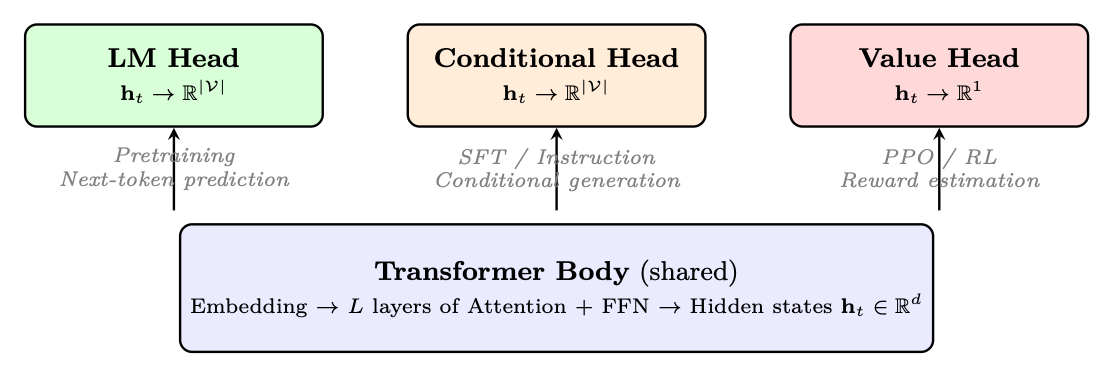
\includegraphics[width=0.85\textwidth]{figures/fig_008_prediction-heads.png}
% \caption{The same transformer backbone supports different tasks by swapping the prediction head. All three heads used in this paper share identical architecture below the final projection layer.}
\caption{同一个 Transformer 主干网络通过更换预测头即可支持不同任务。本文使用的全部三种预测头在最终投影层之下具有完全相同的架构。}
\label{fig:prediction-heads}
\end{figure}

\subsection{语言建模头（预训练阶段）}
\label{language-modeling-head-pretraining}

% The standard LM head projects the final hidden state to vocabulary logits and trains with cross-entropy loss over the next token:
标准的语言建模头（Language Modeling Head, LM Head）将最终隐藏状态投影到词表 logits，并以下一个 token 的交叉熵损失进行训练：

\begin{equation}
P(x_{t+1} | x_{\leq t}) = \text{softmax}(\mathbf{W}_{\text{head}} \cdot \mathbf{h}_t + \mathbf{b})
\end{equation}

% where $\mathbf{W}_{\text{head}} \in \mathbb{R}^{|\mathcal{V}| \times d}$ (often tied with the embedding matrix: $\mathbf{W}_{\text{head}} = \mathbf{E}^T$).
其中 $\mathbf{W}_{\text{head}} \in \mathbb{R}^{|\mathcal{V}| \times d}$（通常与 embedding 矩阵权重共享：$\mathbf{W}_{\text{head}} = \mathbf{E}^T$）。

\begin{keybox}[LM 头的特性]
\begin{itemize}
  % \item \textbf{Training objective}: Causal language modeling (predict next token for every position)
  \item \textbf{训练目标}：因果语言建模（对每个位置预测下一个 token）
  % \item \textbf{Loss}: $\mathcal{L}_{\text{LM}} = -\frac{1}{T}\sum_{t=1}^{T} \log P(x_t | x_{<t})$
  \item \textbf{损失}：$\mathcal{L}_{\text{LM}} = -\frac{1}{T}\sum_{t=1}^{T} \log P(x_t | x_{<t})$
  % \item \textbf{Label}: Every token is both input (shifted right) and target (shifted left)
  \item \textbf{标签}：每个 token 同时作为输入（右移一位）和目标（左移一位）
  % \item \textbf{Used during}: Pretraining on large corpora (trillions of tokens)
  \item \textbf{使用阶段}：在大规模语料上的预训练（万亿级 token）
  % \item \textbf{Key insight}: The model learns general language understanding as a byproduct of next-token prediction
  \item \textbf{关键洞察}：模型在下一 token 预测的副产品中学到通用语言理解能力
\end{itemize}
\end{keybox}

\subsection{条件生成头（SFT / 指令跟随）}
\label{conditional-generation-head-sft-instruction-following}

% For supervised fine-tuning (SFT), the architecture is \emph{identical} to the LM head---the same linear projection to vocabulary logits. The difference is purely in \emph{what we compute loss on}:
对于监督微调（Supervised Fine-Tuning, SFT），其架构与 LM 头\emph{完全相同}——都是将隐藏状态线性投影到词表 logits。区别仅在于\emph{在哪些 token 上计算损失}：

\begin{equation}
\mathcal{L}_{\text{SFT}} = -\frac{1}{|y|}\sum_{t=1}^{|y|} \log P(y_t | x_{\text{prompt}}, y_{<t})
\end{equation}

\begin{keybox}[条件生成头 -- 与 LM 头的关键区别]
\begin{itemize}
  % \item \textbf{Loss masking}: Only compute loss on the \emph{response} tokens, not the prompt/instruction. The prompt provides context but no gradient signal.
  \item \textbf{损失掩码}：只在\emph{回复}的 token 上计算损失，不计算 prompt/指令部分。Prompt 仅提供上下文，不提供梯度信号。
  % \item \textbf{Conditioning}: The model learns to generate responses \emph{conditioned on} specific instruction formats (system prompts, user queries, tool calls).
  \item \textbf{条件化}：模型学会在特定指令格式（system prompt、用户查询、工具调用）的\emph{条件下}生成回复。
  % \item \textbf{Format tokens}: Special tokens (\texttt{<|user|>}, \texttt{<|assistant|>}) guide the model to produce structured outputs.
  \item \textbf{格式 token}：特殊 token（\texttt{<|user|>}、\texttt{<|assistant|>}）引导模型产生结构化输出。
  % \item \textbf{Used during}: SFT on curated instruction-response pairs; also during RL policy generation (the policy head that produces actions/responses).
  \item \textbf{使用阶段}：在精心策划的指令-回复对上进行 SFT；也在强化学习的策略生成阶段使用（即产出动作/回复的策略头）。
\end{itemize}
\end{keybox}

\begin{intuitionbox}[同一个头 -- 不同的训练信号]
% The LM head and SFT head are architecturally identical (same $\mathbf{W}_{\text{head}}$). The only difference is that during SFT, we mask the loss on prompt tokens. This subtle change transforms a general text predictor into a instruction-following assistant. The head learns to ``activate'' different generation modes based on the conditioning context.
LM 头和 SFT 头在架构上完全相同（同一个 $\mathbf{W}_{\text{head}}$）。唯一的区别是 SFT 阶段会掩码掉 prompt token 的损失。这个细微的改动就把一个通用文本预测器转变为一个指令跟随助手。预测头学会根据上下文条件「激活」不同的生成模式。
\end{intuitionbox}

\subsection{价值头（用于 RL 的回归头）}
\label{value-head-regression-for-rl}

% In reinforcement learning (PPO, GRPO), we need to estimate \emph{how good} a state is---this requires a scalar output, not vocabulary logits. The \textbf{value head} replaces the LM projection with a simple regression layer:
在强化学习（PPO、GRPO）中，我们需要估计某个状态\emph{有多好}——这需要一个标量输出，而不是词表 logits。\textbf{价值头（Value Head）}用一个简单的回归层替换了 LM 投影：

\begin{equation}
V(s_t) = \mathbf{w}_{\text{value}}^T \cdot \mathbf{h}_t + b \in \mathbb{R}
\end{equation}

% where $\mathbf{w}_{\text{value}} \in \mathbb{R}^d$ and $b \in \mathbb{R}$.
其中 $\mathbf{w}_{\text{value}} \in \mathbb{R}^d$，$b \in \mathbb{R}$。

\begin{keybox}[价值头的特性]
\begin{itemize}
  % \item \textbf{Output}: Single scalar (expected cumulative reward from this state)
  \item \textbf{输出}：单个标量（从该状态出发的期望累计奖励）
  % \item \textbf{Loss}: MSE between predicted and actual returns: $\mathcal{L}_V = \frac{1}{T}\sum_t (V(s_t) - R_t)^2$
  \item \textbf{损失}：预测回报与真实回报之间的均方误差：$\mathcal{L}_V = \frac{1}{T}\sum_t (V(s_t) - R_t)^2$
  % \item \textbf{Architecture}: Linear layer $\mathbb{R}^d \to \mathbb{R}^1$ (sometimes with a small MLP: $d \to 256 \to 1$)
  \item \textbf{架构}：线性层 $\mathbb{R}^d \to \mathbb{R}^1$（有时会用一个小型 MLP：$d \to 256 \to 1$）
  % \item \textbf{Backbone sharing}: Often shares the transformer body with the policy (with a separate value head), or uses a completely separate critic network
  \item \textbf{主干共享}：通常与策略共享 Transformer 主干（但有独立的价值头），也可能使用完全独立的 critic 网络
  % \item \textbf{Used during}: PPO advantage estimation (GAE), reward model scoring
  \item \textbf{使用阶段}：PPO 优势估计（GAE）、奖励模型评分
\end{itemize}
\end{keybox}

\subsection{预测头选择总览}
\label{head-selection-summary}

\begin{table}[ht!]
\centering\small
% \caption{Prediction heads used throughout this paper and their training contexts.}
\caption{本文使用的各类预测头及其训练场景。}
\noindent\begin{tabularx}{\linewidth}{@{}l Z{0.48} Z{1.29} Z{0.61} Z{1.62}@{}}
\toprule
% \textbf{Head} & \textbf{Output} & \textbf{Loss} & \textbf{Stage} & \textbf{Purpose} \\
\textbf{预测头} & \textbf{输出} & \textbf{损失} & \textbf{阶段} & \textbf{用途} \\
\midrule
% LM Head & $\mathbb{R}^{|\mathcal{V}|}$ & Cross-entropy (all tokens) & Pretraining & Learn language from raw text \\
LM Head & $\mathbb{R}^{|\mathcal{V}|}$ & 交叉熵（所有 token） & 预训练 & 从原始文本学习语言 \\
% Conditional Head & $\mathbb{R}^{|\mathcal{V}|}$ & Cross-entropy (response only) & SFT & Learn to follow instructions \\
Conditional Head & $\mathbb{R}^{|\mathcal{V}|}$ & 交叉熵（仅回复部分） & SFT & 学习跟随指令 \\
% Value Head & $\mathbb{R}^1$ & MSE & RL (PPO) & Estimate state value for advantage \\
Value Head & $\mathbb{R}^1$ & MSE & RL (PPO) & 估计状态价值以计算优势 \\
% Reward Head & $\mathbb{R}^1$ & Pairwise ranking & RM training & Score response quality \\
Reward Head & $\mathbb{R}^1$ & 成对排序 & 奖励模型训练 & 给回复质量打分 \\
\bottomrule
\end{tabularx}
\end{table}

\begin{warningbox}[预测头初始化很重要]
% When adding a value head to a pretrained LM, initialize it near zero (small random weights). If initialized with large values, the initial value estimates will be wildly wrong, causing huge advantages and unstable PPO updates. Common practice: initialize the final linear layer with $\mathcal{N}(0, 1/\sqrt{d})$ or simply zeros.
为预训练 LM 添加价值头时，应将其初始化为接近零的小随机权重。若初始化值过大，初始价值估计会严重偏离，导致优势值过大、PPO 更新不稳定。常见做法：将最后一层线性层用 $\mathcal{N}(0, 1/\sqrt{d})$ 初始化，或直接置零。
\end{warningbox}

\subsection{HuggingFace 实现}
\label{huggingface-implementation}

% \begin{lstlisting}[style=pythonstyle, caption={Loading and using different prediction heads with HuggingFace.}]
\begin{lstlisting}[style=pythonstyle, caption={使用 HuggingFace 加载与使用不同的预测头。}]
from transformers import (
    AutoModelForCausalLM,          # LM 头（预训练 + SFT）
    AutoModelForSequenceClassification,  # 奖励头
    AutoTokenizer,
)
from trl import AutoModelForCausalLMWithValueHead  # 价值头（PPO）
import torch

model_name = "meta-llama/Llama-3.1-8B-Instruct"
tokenizer = AutoTokenizer.from_pretrained(model_name)

# === 1. LM 头（预训练 / SFT）===
# 默认的 CausalLM 模型——将隐藏状态投影到词表 logits
lm_model = AutoModelForCausalLM.from_pretrained(
    model_name,
    torch_dtype=torch.bfloat16,
    device_map="auto",
)
# lm_model.lm_head: Linear(hidden_size -> vocab_size)
# 输出：形状为 (batch, seq_len, vocab_size) 的 logits

inputs = tokenizer("The capital of France is", return_tensors="pt")
outputs = lm_model(**inputs)
next_token_logits = outputs.logits[:, -1, :]  # (batch, vocab_size)
probs = torch.softmax(next_token_logits, dim=-1)

# === 2. 条件生成头（SFT）===
# 架构上与 LM 头完全相同——区别在于损失掩码
# SFT 时只在回复 token 上计算损失：
messages = [
    {"role": "user", "content": "What is 2+2?"},
    {"role": "assistant", "content": "4"},
]
formatted = tokenizer.apply_chat_template(messages, return_tensors="pt")
labels = formatted.clone()
# 掩码掉 prompt token（设为 -100，交叉熵会忽略它们）
prompt_len = len(tokenizer.apply_chat_template(messages[:1]))
labels[:, :prompt_len] = -100
loss = lm_model(input_ids=formatted, labels=labels).loss

# === 3. 价值头（PPO Critic）===
# 在 LM 主干之上加一个 Linear(hidden_size -> 1)
value_model = AutoModelForCausalLMWithValueHead.from_pretrained(
    model_name,
    torch_dtype=torch.bfloat16,
    device_map="auto",
)
# value_model.v_head: Linear(hidden_size -> 1)
# 同时返回 LM logits 和每个 token 的价值估计

inputs = tokenizer("Explain quantum computing", return_tensors="pt")
lm_logits, loss, values = value_model(
    **inputs, return_dict=False
)
# values 形状：(batch, seq_len, 1)——每个 token 一个标量估计

# === 4. 奖励头（奖励模型）===
# 分类头：在最后一个 token 上接 Linear(hidden_size -> 1)
reward_model = AutoModelForSequenceClassification.from_pretrained(
    model_name,
    num_labels=1,              # 单标量输出
    torch_dtype=torch.bfloat16,
    device_map="auto",
)
# 通过池化最后一个 token 的隐藏状态对整个序列打分
inputs = tokenizer("Good response here", return_tensors="pt")
reward_score = reward_model(**inputs).logits  # 形状：(batch, 1)
\end{lstlisting}

\begin{intuitionbox}[权重共享：LM 头 = embedding 矩阵的转置]
% Most modern LLMs \emph{tie} the LM head weights with the input embedding matrix: \texttt{lm\_head.weight = model.embed\_tokens.weight}. This means the LM head is \emph{not} a separately learned layer---it reuses the embedding table. Benefits: fewer parameters ($|\mathcal{V}| \times d$ saved), better generalization, and the geometric structure of the embedding space directly determines token probabilities. You can verify this in HuggingFace: \texttt{model.lm\_head.weight is model.model.embed\_tokens.weight} returns \texttt{True} for most models.
大多数现代 LLM 会将 LM 头的权重与输入 embedding 矩阵\emph{共享（tie）}：\texttt{lm\_head.weight = model.embed\_tokens.weight}。这意味着 LM 头\emph{并非}独立学习的一层——它直接复用了 embedding 表。好处包括：参数更少（节省 $|\mathcal{V}| \times d$）、泛化更好，并且 embedding 空间的几何结构直接决定了 token 概率。你可以在 HuggingFace 中验证这一点：对大多数模型而言，\texttt{model.lm\_head.weight is model.model.embed\_tokens.weight} 会返回 \texttt{True}。
\end{intuitionbox}

\newpage
\section{LLM 训练的优化理论}
\label{optimization-theory-for-llm-training}

% Training a large language model means finding the set of parameters $\theta$ (billions of weights) that minimizes the loss function $\mathcal{L}(\theta)$ --- typically the negative log-likelihood of the next token. This is an optimization problem in extraordinarily high-dimensional space, and the algorithm used to navigate this space determines whether training succeeds, diverges, or stalls.
训练一个大语言模型意味着寻找一组参数 $\theta$（数十亿个权重），使损失函数 $\mathcal{L}(\theta)$ ——通常是下一个 token 的负对数似然——最小化。这是一个在极高维空间中的优化问题，用来在该空间中导航的算法直接决定了训练是成功、发散还是停滞。

\subsection{梯度下降：基础}
\label{gradient-descent-the-foundation}

\paragraph{什么是梯度？}
\label{what-is-a-gradient}

% The gradient $\nabla_\theta \mathcal{L}$ is a vector that points in the direction of \emph{steepest increase} of the loss. Each component $\frac{\partial \mathcal{L}}{\partial \theta_i}$ tells us how much the loss would change if we slightly increased parameter $\theta_i$. To \emph{decrease} the loss, we move in the opposite direction:
梯度 $\nabla_\theta \mathcal{L}$ 是一个指向损失函数\emph{最陡上升方向}的向量。每个分量 $\frac{\partial \mathcal{L}}{\partial \theta_i}$ 告诉我们：如果对参数 $\theta_i$ 略微增加一点，损失会变化多少。为了\emph{降低}损失，我们沿相反方向移动：

\begin{equation}
\theta_{t+1} = \theta_t - \eta \nabla_\theta \mathcal{L}(\theta_t)
\end{equation}

% where $\eta > 0$ is the \textbf{learning rate} --- the step size. This is \textbf{gradient descent}~\cite{rumelhart1986learning}.
其中 $\eta > 0$ 是\textbf{学习率（Learning Rate）}——也就是步长。这就是\textbf{梯度下降（Gradient Descent）}~\cite{rumelhart1986learning}。

\begin{figure}[ht!]
\centering
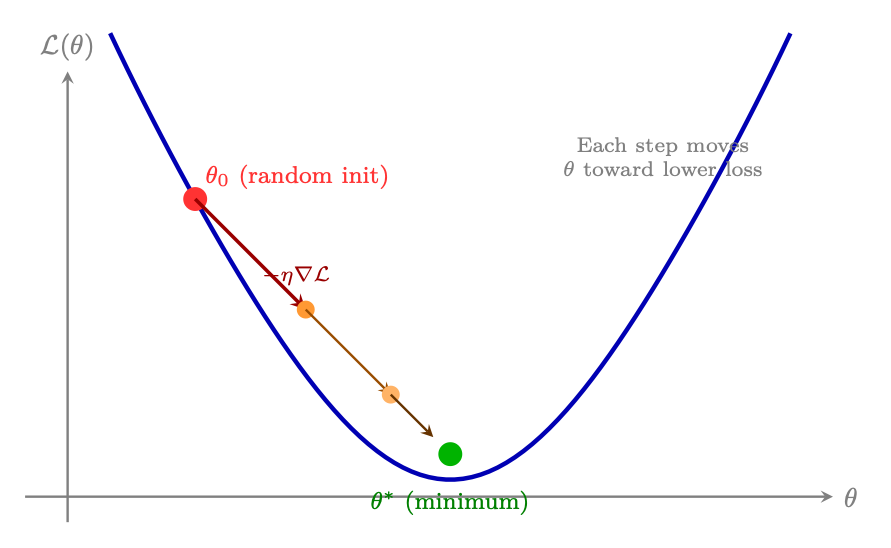
\includegraphics[width=0.7\textwidth]{figures/fig_009_fig9.png}
% \caption{Gradient descent: starting from a random initialization $\theta_0$, each step moves the parameters in the direction that reduces the loss, with step size controlled by the learning rate $\eta$. The process converges toward a (local) minimum.}
\caption{梯度下降：从随机初始化 $\theta_0$ 开始，每一步都将参数沿降低损失的方向移动，步长由学习率 $\eta$ 控制。该过程会向某个（局部）最小值收敛。}
\end{figure}

\paragraph{为何全梯度下降不可行。}
\label{why-full-gradient-descent-is-impractical.}

% Computing the exact gradient requires evaluating the loss over the \emph{entire} training dataset (trillions of tokens for LLMs). This is computationally prohibitive --- a single gradient step would require a full pass over all data.
计算精确梯度需要在\emph{整个}训练集上评估损失（对 LLM 而言是万亿级 token），计算开销极其高昂——单步梯度更新就需要遍历全部数据。

\paragraph{随机梯度下降（Stochastic Gradient Descent，SGD）。}
\label{stochastic-gradient-descent-sgd.}

% The solution: estimate the gradient from a small random subset (\textbf{mini-batch}) of the data~\cite{robbins1951stochastic}:
解决办法是：用一个小的随机数据子集（\textbf{小批量，mini-batch}）来估计梯度~\cite{robbins1951stochastic}：
\[
\nabla_\theta \mathcal{L}(\theta) \approx \frac{1}{B}\sum_{i=1}^{B} \nabla_\theta \ell(\theta; x_i)
\]
% where $B$ is the batch size (typically 1K--4M tokens for LLMs). The mini-batch gradient is a \emph{noisy but unbiased} estimate of the true gradient.
其中 $B$ 是批大小（对 LLM 通常是 1K--4M 个 token）。小批量梯度是真实梯度的\emph{含噪但无偏}的估计。

\begin{keybox}[为何小批量 SGD 有效]
\begin{itemize}
  % \item \textbf{Computational efficiency}: Each step costs $O(B)$ instead of $O(N_{\text{total}})$. With $B = 4096$ tokens and 15T total tokens, each step is $\sim$4 billion$\times$ cheaper.
  \item \textbf{计算效率}：每步开销是 $O(B)$ 而非 $O(N_{\text{total}})$。当 $B = 4096$ 而总 token 为 15T 时，每步开销约便宜 40 亿倍。
  % \item \textbf{Noise as regularization}: The stochastic noise helps escape sharp local minima, finding flatter regions that generalize better.
  \item \textbf{噪声即正则化}：随机噪声有助于逃离尖锐的局部极小值，找到泛化性更好的平坦区域。
  % \item \textbf{GPU utilization}: Mini-batches are large enough to saturate GPU parallelism (matrix multiplications become compute-bound rather than memory-bound).
  \item \textbf{GPU 利用率}：小批量足够大，能充分占满 GPU 并行度（矩阵乘法变为计算受限而非显存受限）。
  % \item \textbf{Convergence}: Theoretically converges to a local minimum at rate $O(1/\sqrt{T})$ (slower than exact GD’s $O(1/T)$, but each step is millions of times cheaper).
  \item \textbf{收敛性}：理论上以 $O(1/\sqrt{T})$ 的速率收敛到局部极小值（比精确 GD 的 $O(1/T)$ 慢，但每步开销便宜数百万倍）。
\end{itemize}
\end{keybox}

\paragraph{从 SGD 到自适应方法。}
\label{from-sgd-to-adaptive-methods.}

% While SGD with momentum works well for vision models (CNNs), LLM training requires \textbf{adaptive optimizers} --- algorithms that maintain a per-parameter learning rate.
带动量的 SGD 对视觉模型（CNN）效果不错，但 LLM 训练需要\textbf{自适应优化器（Adaptive Optimizer）}——即为每个参数维护各自学习率的算法。

\subsection{为何朴素 SGD 在 LLM 上失效}
\label{why-vanilla-sgd-fails-for-llms}

% Stochastic Gradient Descent updates weights as:
随机梯度下降按下式更新权重：
\[
\theta_{t+1} = \theta_t - \eta \nabla_\theta \mathcal{L}(\theta_t)
\]

\begin{warningbox}[SGD 在 LLM 上的问题]
\begin{itemize}
  % \item \textbf{Different gradient scales per layer:} Early layers in a transformer have much smaller gradients than later layers (vanishing gradients). A single learning rate $\eta$ is too large for some parameters and too small for others.
  \item \textbf{各层梯度尺度不同：}Transformer 早期层的梯度远小于后期层（梯度消失）。单一学习率 $\eta$ 对一些参数过大，对另一些参数又过小。
  % \item \textbf{Sparse gradients:} Embedding layers receive gradients only for tokens in the current batch. Most embedding rows have zero gradient. SGD with momentum wastes momentum on zero-gradient rows.
  \item \textbf{稀疏梯度：}embedding 层只对当前批次出现的 token 有梯度，大部分行的梯度为零。带动量的 SGD 会在零梯度行上浪费动量。
  % \item \textbf{Saddle points:} High-dimensional loss landscapes have many saddle points. SGD can stall; adaptive methods escape faster.
  \item \textbf{鞍点：}高维损失曲面存在大量鞍点。SGD 可能停滞，而自适应方法能更快逃脱。
  % \item \textbf{Sensitivity to learning rate:} SGD requires careful tuning; a 2$\times$ change in $\eta$ can cause divergence.
  \item \textbf{对学习率敏感：}SGD 需要仔细调参；$\eta$ 变化 2 倍就可能导致发散。
\end{itemize}
\end{warningbox}

\subsection{Adam --- 自适应矩估计（Adaptive Moment Estimation）}
\label{adam-adaptive-moment-estimation}

% Adam~\cite{kingma2015adam} maintains per-parameter estimates of the first moment (mean of gradients) and second moment (uncentered variance of gradients).
Adam~\cite{kingma2015adam} 为每个参数维护梯度一阶矩（均值）与二阶矩（非中心化方差）的估计。

\begin{keybox}[Adam 更新方程]
% Given gradient $g_t = \nabla_\theta \mathcal{L}(\theta_t)$, hyperparameters $\beta_1, \beta_2, \epsilon, \eta$:
给定梯度 $g_t = \nabla_\theta \mathcal{L}(\theta_t)$ 与超参数 $\beta_1, \beta_2, \epsilon, \eta$：

% \textbf{Step 1 -- Update biased first moment estimate:}
\textbf{第 1 步 -- 更新有偏一阶矩估计：}
\[
m_t = \beta_1 m_{t-1} + (1 - \beta_1) g_t
\]

% \textbf{Step 2 -- Update biased second moment estimate:}
\textbf{第 2 步 -- 更新有偏二阶矩估计：}
\[
v_t = \beta_2 v_{t-1} + (1 - \beta_2) g_t^2
\]

% \textbf{Step 3 -- Bias correction:}
\textbf{第 3 步 -- 偏差校正：}
\[
\hat{m}_t = \frac{m_t}{1 - \beta_1^t}, \qquad \hat{v}_t = \frac{v_t}{1 - \beta_2^t}
\]

% \textbf{Step 4 -- Parameter update:}
\textbf{第 4 步 -- 参数更新：}
\[
\theta_{t+1} = \theta_t - \eta \cdot \frac{\hat{m}_t}{\sqrt{\hat{v}_t} + \epsilon}
\]

% \textbf{Typical values:} $\beta_1 = 0.9$, $\beta_2 = 0.95$ or $0.999$, $\epsilon = 10^{-8}$, $\eta = 10^{-4}$ to $10^{-5}$.
\textbf{典型取值：}$\beta_1 = 0.9$，$\beta_2 = 0.95$ 或 $0.999$，$\epsilon = 10^{-8}$，$\eta = 10^{-4}$ 至 $10^{-5}$。
\end{keybox}

\newpage
\begin{intuitionbox}[每一项的作用]
\begin{itemize}
  % \item $m_t$ (\textbf{momentum}): Exponential moving average of gradients. Smooths out noisy gradient estimates. $\beta_1 = 0.9$ means the current gradient contributes 10\% and the history contributes 90\%.
  \item $m_t$（\textbf{动量}）：梯度的指数移动平均，可平滑噪声梯度估计。$\beta_1 = 0.9$ 意味着当前梯度贡献 10\%，历史贡献 90\%。
  % \item $v_t$ (\textbf{adaptive LR}): EMA of squared gradients. Parameters with consistently large gradients get a smaller effective learning rate ($\eta / \sqrt{v_t}$). Parameters with small gradients get a larger effective LR. This is the key to handling different gradient scales per layer.
  \item $v_t$（\textbf{自适应学习率}）：梯度平方的 EMA。梯度持续较大的参数获得较小的有效学习率（$\eta / \sqrt{v_t}$）；梯度较小的参数获得较大的有效学习率。这是应对各层梯度尺度差异的关键。
  % \item $\hat{m}_t, \hat{v}_t$ (\textbf{bias correction}): At $t=1$, $m_1 = (1-\beta_1)g_1$ is much smaller than the true mean. Dividing by $(1-\beta_1^t)$ corrects this initialization bias. Without it, early steps are too small.
  \item $\hat{m}_t, \hat{v}_t$（\textbf{偏差校正}）：在 $t=1$ 时，$m_1 = (1-\beta_1)g_1$ 远小于真实均值。除以 $(1-\beta_1^t)$ 可以校正这种初始化偏差。如果不做校正，早期更新步长会过小。
  % \item $\epsilon$ (\textbf{numerical stability}): Prevents division by zero. Also acts as a floor on the effective learning rate.
  \item $\epsilon$（\textbf{数值稳定性}）：防止除零；同时也作为有效学习率的下限。
\end{itemize}
\end{intuitionbox}

\subsection{AdamW --- 解耦权重衰减（Decoupled Weight Decay, AdamW）}
\label{adamw-decoupled-weight-decay}

% AdamW~\cite{loshchilov2019adamw} fixes a subtle but important issue with how weight decay interacts with adaptive optimizers.
AdamW~\cite{loshchilov2019adamw} 修正了权重衰减与自适应优化器交互时一个细微但重要的问题。

\begin{keybox}[为何在 Adam 中 L2 正则 $\neq$ 权重衰减]
% With L2 regularization, the loss becomes $\mathcal{L} + \frac{\lambda}{2}\|\theta\|^2$, so the gradient is $g_t + \lambda \theta_t$. In Adam, this regularization gradient is \emph{scaled by the adaptive factor} $1/\sqrt{\hat{v}_t}$:
在 L2 正则化下，损失变为 $\mathcal{L} + \frac{\lambda}{2}\|\theta\|^2$，因此梯度为 $g_t + \lambda \theta_t$。在 Adam 中，这部分正则化梯度会\emph{被自适应因子} $1/\sqrt{\hat{v}_t}$ \emph{缩放}：
\[
\theta_{t+1} = \theta_t - \eta \cdot \frac{\hat{m}_t + \lambda \theta_t}{\sqrt{\hat{v}_t} + \epsilon}
\]
% Parameters with large $v_t$ (large gradient variance) get \emph{less} regularization. This is not what we want -- weight decay should be uniform.
$v_t$ 较大（梯度方差大）的参数受到的正则化反而\emph{更弱}。这并不是我们想要的——权重衰减本应是均匀的。
\end{keybox}

\begin{keybox}[AdamW -- 解耦权重衰减]
% AdamW (Loshchilov \& Hutter, 2017) applies weight decay \emph{directly} to the parameters, outside the adaptive scaling:
AdamW（Loshchilov \& Hutter, 2017）将权重衰减\emph{直接}作用于参数本身，置于自适应缩放之外：
\[
\theta_{t+1} = \theta_t - \eta \cdot \frac{\hat{m}_t}{\sqrt{\hat{v}_t} + \epsilon}
  - \eta \lambda \theta_t
\]
% The weight decay term $\eta \lambda \theta_t$ is not divided by $\sqrt{\hat{v}_t}$. This gives uniform regularization across all parameters regardless of their gradient history.
权重衰减项 $\eta \lambda \theta_t$ 不再被 $\sqrt{\hat{v}_t}$ 缩放。这样无论参数的梯度历史如何，所有参数都能获得均匀的正则化。

% \textbf{Typical value:} $\lambda = 0.1$ for LLM training.
\textbf{典型取值：}LLM 训练时 $\lambda = 0.1$。
\end{keybox}

\begin{warningbox}[对 LLM 始终使用 AdamW -- 不要用纯 Adam]
% The difference between Adam and AdamW is subtle but matters. With Adam + L2, the effective weight decay is stronger for parameters with small gradient variance (e.g., biases, LayerNorm parameters) and weaker for parameters with large gradient variance (e.g., attention weights). AdamW gives the intended uniform regularization. Most frameworks default to AdamW; double-check your optimizer class.
Adam 与 AdamW 的差别虽细微但很重要。使用 Adam + L2 时，梯度方差小的参数（如 bias、LayerNorm 参数）受到更强的权重衰减，梯度方差大的参数（如 attention 权重）受到的衰减更弱。AdamW 才能提供我们想要的均匀正则化。大多数框架默认使用 AdamW；务必确认你的优化器类。
\end{warningbox}

\newpage
\subsection{学习率 --- 最重要的超参数}
\label{learning-rate-the-most-important-hyperparameter}

\begin{keybox}[各训练阶段的典型学习率]
\begin{center}
\begin{tabular}{@{}l l l@{}}
\toprule
% \textbf{Phase} & \textbf{Typical LR} & \textbf{Notes} \\
\textbf{阶段} & \textbf{典型学习率} & \textbf{备注} \\
\midrule
% Pretraining (from scratch) & $1\text{e-}4$ to $3\text{e-}4$ & Large model, large batch \\
从零预训练 & $1\text{e-}4$ 至 $3\text{e-}4$ & 大模型、大批量 \\
% Continued pretraining & $1\text{e-}5$ to $1\text{e-}4$ & Smaller LR to preserve knowledge \\
继续预训练 & $1\text{e-}5$ 至 $1\text{e-}4$ & 更小学习率以保留已有知识 \\
% SFT (supervised fine-tune) & $1\text{e-}5$ to $2\text{e-}5$ & Standard range \\
SFT（监督微调） & $1\text{e-}5$ 至 $2\text{e-}5$ & 标准区间 \\
% LoRA fine-tuning & $1\text{e-}4$ to $3\text{e-}4$ & Higher LR for adapter weights \\
LoRA 微调 & $1\text{e-}4$ 至 $3\text{e-}4$ & 适配器权重需用更高学习率 \\
\bottomrule
\end{tabular}
\end{center}

\smallskip
% \noindent\emph{For RL learning rates (PPO, DPO, GRPO) see §\ref{sec:rl-optimizer-config}.}
\noindent\emph{有关 RL 学习率（PPO、DPO、GRPO）请参见 §\ref{sec:rl-optimizer-config}。}
\end{keybox}

\subsection{学习率预热（Warmup）}
\label{learning-rate-warmup}

\begin{keybox}[为何需要预热]
% At the start of training, $v_t$ (the second moment estimate) is initialized to zero. After bias correction: $\hat{v}_t = v_t / (1 - \beta_2^t)$. At $t=1$ with $\beta_2 = 0.999$: $\hat{v}_1 = v_1 / (1 - 0.999) = 1000 v_1$. This means the effective learning rate is $\eta / \sqrt{1000 v_1}$ -- much smaller than intended.
训练开始时，$v_t$（二阶矩估计）被初始化为零。偏差校正后：$\hat{v}_t = v_t / (1 - \beta_2^t)$。在 $t=1$、$\beta_2 = 0.999$ 时：$\hat{v}_1 = v_1 / (1 - 0.999) = 1000 v_1$。这意味着有效学习率是 $\eta / \sqrt{1000 v_1}$，远小于预期。

% However, if the first gradient is unusually large (common at initialization), the second moment estimate can be dominated by this outlier, causing erratic early steps. Warmup mitigates this by starting with a very small LR and gradually increasing it, giving $v_t$ time to accumulate a reliable estimate.
另一方面，如果第一步的梯度异常大（在初始化时常见），二阶矩估计会被这个离群值主导，导致早期更新极不稳定。预热（Warmup）通过从极小的学习率开始、逐步增大来缓解这一问题，让 $v_t$ 有时间积累一个可靠的估计。
\end{keybox}

\begin{itemize}
  % \item \textbf{Linear warmup:} $\eta_t = \eta_{\max} \times t / T_{\text{warmup}}$
  \item \textbf{线性预热：}$\eta_t = \eta_{\max} \times t / T_{\text{warmup}}$
  % \item \textbf{Typical warmup duration:} 1--5\% of total steps for pretraining; 3--10\% for fine-tuning (shorter runs need proportionally more warmup)
  \item \textbf{典型预热时长：}预训练为总步数的 1--5\%；微调为 3--10\%（更短的训练任务通常需要按比例更长的预热）
  % \item \textbf{For SFT:} 50--200 warmup steps is typical
  \item \textbf{SFT 场景：}通常预热 50--200 步
\end{itemize}

\subsection{学习率调度策略}
\label{learning-rate-schedules}

\begin{figure}[ht!]
\centering
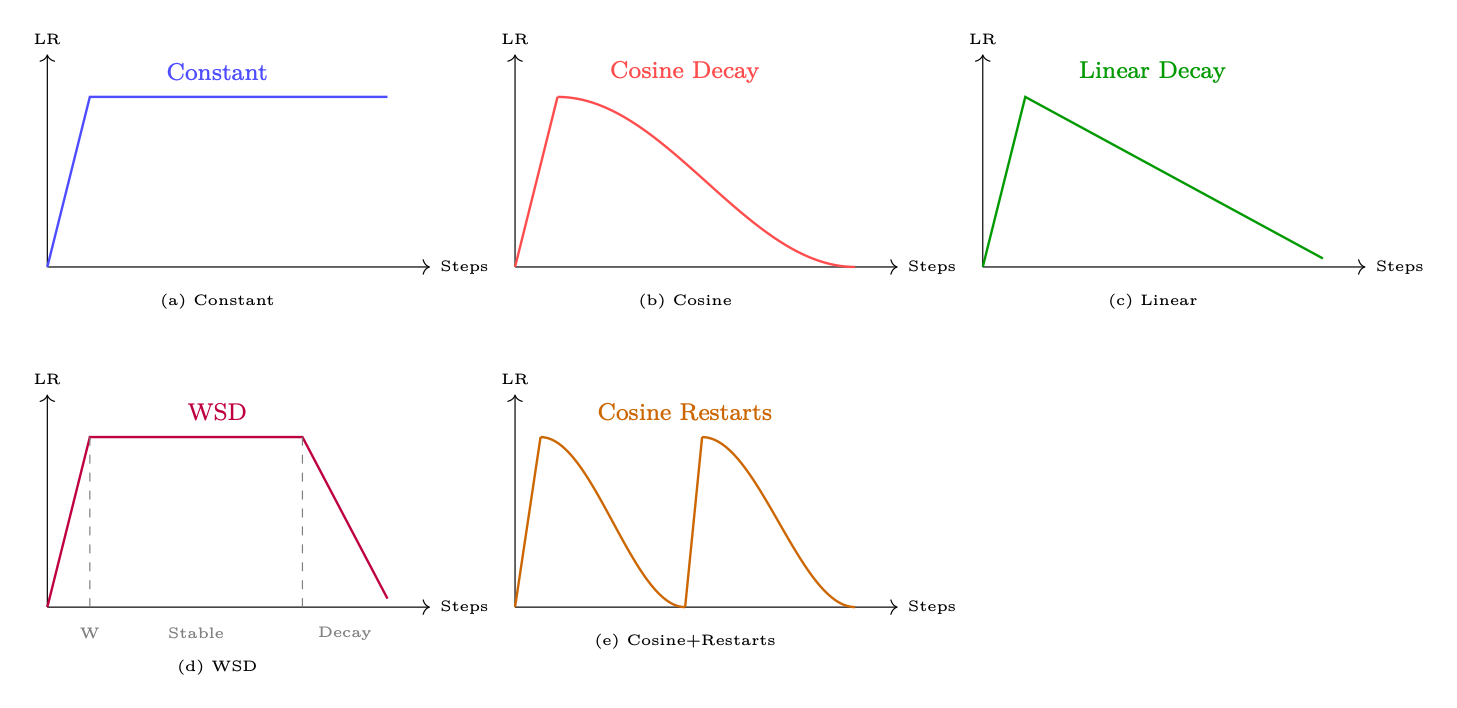
\includegraphics[width=0.85\textwidth]{figures/fig_010_fig10.png}
% \caption{Common learning rate schedules. All include a linear warmup phase. WSD (Warmup-Stable-Decay) is the emerging standard for pretraining.}
\caption{常见学习率调度。所有调度都包含一个线性预热阶段。WSD（Warmup-Stable-Decay）正成为预训练的事实标准。}
\end{figure}

\paragraph{(a) 恒定调度（Constant）。}
\label{a-constant.}

% Simplest schedule. Good for short fine-tuning runs where you want to avoid over-decaying the LR. Risk: no annealing means the model may not converge to the sharpest minimum.
最简单的调度。适合短期微调，以避免学习率过度衰减。风险在于：缺乏退火意味着模型可能无法收敛到最尖锐的最小值。

\paragraph{(b) 余弦衰减（Cosine Decay）。}
\label{b-cosine-decay.}

\[
\eta_t = \eta_{\min} + \frac{1}{2}(\eta_{\max} - \eta_{\min})
  \left(1 + \cos\!\left(\frac{t - T_{\text{warmup}}}{T - T_{\text{warmup}}} \pi\right)\right)
\]
% Standard for pretraining and SFT. Smooth decay avoids abrupt LR changes. $\eta_{\min}$ is typically $\eta_{\max} / 10$.
预训练与 SFT 的标准选择。平滑衰减避免了学习率的突变。$\eta_{\min}$ 通常取 $\eta_{\max} / 10$。

\paragraph{(c) 线性衰减（Linear Decay）。}
\label{c-linear-decay.}

% Simpler than cosine, similar empirical results. Preferred when you want predictable LR at any step.
比余弦更简单，经验效果相近。当你希望任意步的学习率都可预测时优先选用。

\paragraph{(d) WSD --- 预热-稳定-衰减（Warmup-Stable-Decay, WSD）。}
\label{d-wsd-warmup-stable-decay.}

% The new standard for large-scale pretraining~\cite{hu2024minicpm, grattafiori2024llama3}. Three phases:
大规模预训练的新标准~\cite{hu2024minicpm, grattafiori2024llama3}。包含三个阶段：

\begin{enumerate}
  % \item \textbf{Warmup:} Linear ramp to $\eta_{\max}$ (1--5\% of steps)
  \item \textbf{预热：}线性升至 $\eta_{\max}$（占总步数的 1--5\%）
  % \item \textbf{Stable:} Constant $\eta_{\max}$ for the majority of training
  \item \textbf{稳定：}在训练的大部分时间保持恒定的 $\eta_{\max}$
  % \item \textbf{Decay:} Fast cosine or linear decay to $\eta_{\min}$ (last 10--20\% of steps)
  \item \textbf{衰减：}以快速余弦或线性方式衰减到 $\eta_{\min}$（最后 10--20\% 的步数）
\end{enumerate}

% Key advantage: the stable phase allows checkpointing at any point and continuing training. The decay phase can be applied at the end of any run.
核心优势在于：稳定阶段允许在任意时刻打 checkpoint 并继续训练；而衰减阶段可在任一训练任务结束时再施加。

\paragraph{(e) 带重启的余弦调度 --- 带重启的随机梯度下降（Stochastic Gradient Descent with Warm Restarts, SGDR）。}
\label{e-cosine-with-restarts-sgdr.}

% Periodic restarts reset the LR to $\eta_{\max}$. Can help escape local minima. Less common for LLMs; more useful for smaller models.
周期性重启会将学习率重置为 $\eta_{\max}$，有助于逃离局部极小值。在 LLM 中并不常用，更适合较小的模型。

\subsection{梯度裁剪（Gradient Clipping）}
\label{gradient-clipping}

\begin{keybox}[梯度裁剪（Gradient Clipping）]
% Gradient clipping rescales the gradient if its global norm exceeds a threshold:
当梯度的全局范数超过某阈值时，梯度裁剪会对其重新缩放：
\[
g_t \leftarrow g_t \cdot \min\!\left(1,\; \frac{\tau}{\|g_t\|_2}\right)
\]
% where $\tau$ is \texttt{max\_grad\_norm} (typically 1.0).
其中 $\tau$ 是 \texttt{max\_grad\_norm}（通常取 1.0）。
\end{keybox}

\begin{intuitionbox}[梯度裁剪 vs.\ 降低学习率]
% Gradient clipping and reducing the learning rate both limit the size of parameter updates. The difference: clipping preserves the \emph{direction} of the gradient (just scales the magnitude), while a smaller LR scales all updates uniformly. Clipping is better for handling occasional large gradients without slowing down normal training steps.
梯度裁剪与降低学习率都能限制参数更新的幅度。区别在于：裁剪保留梯度的\emph{方向}（只是缩放幅度），而较小的学习率会对所有更新一视同仁地缩放。裁剪更适合处理偶发的大梯度，同时不会拖慢正常训练步的速度。
\end{intuitionbox}

\subsubsection{综合实践：HuggingFace 优化器配置}
\label{putting-it-together-huggingface-optimizer-configuration}

% The following snippet shows how the concepts from this section---AdamW with decoupled weight decay (§1.6.6), cosine learning-rate scheduling with linear warmup (§1.6.7), and gradient clipping (§1.6.8)---come together in practice using the HuggingFace \texttt{transformers} library.
下面的代码片段展示了本节中各概念——带解耦权重衰减的 AdamW（§1.6.6）、带线性预热的余弦学习率调度（§1.6.7）和梯度裁剪（§1.6.8）——如何借助 HuggingFace \texttt{transformers} 库在实践中结合起来。

% \begin{lstlisting}[style=pythonstyle, caption={Complete optimizer configuration combining AdamW -- cosine schedule -- and gradient clipping.}]
\begin{lstlisting}[style=pythonstyle, caption={将 AdamW、余弦调度与梯度裁剪整合在一起的完整优化器配置。}]
from transformers import TrainingArguments, Trainer
from transformers import get_cosine_schedule_with_warmup
import torch

# --- 方案 1：使用 TrainingArguments（推荐）---
training_args = TrainingArguments(
    output_dir="./checkpoints",

    # AdamW 优化器（解耦权重衰减，§1.6.6）
    optim="adamw_torch",
    learning_rate=2e-5,           # 预热后的峰值学习率
    adam_beta1=0.9,               # 一阶矩衰减
    adam_beta2=0.999,             # 二阶矩衰减
    adam_epsilon=1e-8,            # 数值稳定项
    weight_decay=0.01,           # 解耦 L2 惩罚

    # 学习率调度（§1.6.7）
    lr_scheduler_type="cosine",  # 余弦衰减至 0
    warmup_ratio=0.1,            # 10% 步数用于线性预热

    # 梯度裁剪（§1.6.8）
    max_grad_norm=1.0,           # 按全局 L2 范数裁剪

    # 混合精度（§1.6.9）
    bf16=True,                   # 在 Ampere+ GPU 上使用 BFloat16

    # 训练时长
    num_train_epochs=3,
    per_device_train_batch_size=8,
    gradient_accumulation_steps=4,  # 有效批量 = 8*4 = 32
)

trainer = Trainer(
    model=model,
    args=training_args,
    train_dataset=dataset,
)
trainer.train()

# --- 方案 2：手动控制（适用于自定义训练循环）---
from torch.optim import AdamW

# 权重衰减分组（不对 bias / norm 做正则化）
no_decay = ["bias", "LayerNorm.weight", "layernorm.weight"]
param_groups = [
    {
        "params": [p for n, p in model.named_parameters()
                   if not any(nd in n for nd in no_decay)],
        "weight_decay": 0.01,
    },
    {
        "params": [p for n, p in model.named_parameters()
                   if any(nd in n for nd in no_decay)],
        "weight_decay": 0.0,
    },
]

optimizer = AdamW(param_groups, lr=2e-5, betas=(0.9, 0.999))

# 带线性预热的余弦调度
total_steps = len(train_dataloader) * num_epochs
warmup_steps = int(0.1 * total_steps)
scheduler = get_cosine_schedule_with_warmup(
    optimizer,
    num_warmup_steps=warmup_steps,
    num_training_steps=total_steps,
)

# 带梯度裁剪的训练循环
for batch in train_dataloader:
    outputs = model(**batch)
    loss = outputs.loss
    loss.backward()

    # 在 optimizer.step() 之前裁剪梯度
    torch.nn.utils.clip_grad_norm_(model.parameters(), max_norm=1.0)

    optimizer.step()
    scheduler.step()
    optimizer.zero_grad()
\end{lstlisting}

\begin{keybox}[实践要点]
\begin{itemize}
  % \item \textbf{Weight decay exclusion}: bias terms and layer-norm weights should not be regularized---they have few parameters and regularizing them hurts performance \cite{loshchilov2019adamw}.
  \item \textbf{权重衰减排除}：bias 项和 LayerNorm 权重不应被正则化——它们参数很少，对其加正则反而损害性能 \cite{loshchilov2019adamw}。
  % \item \textbf{Warmup ratio}: 5--10\% of total steps is standard; too little warmup with a high LR can destabilize early training.
  \item \textbf{预热比例}：通常为总步数的 5--10\%；预热不足配合高学习率会使早期训练不稳定。
  % \item \textbf{Gradient accumulation}: simulates larger batches on limited GPU memory; clipping applies to the \emph{accumulated} gradient.
  \item \textbf{梯度累积}：在显存受限时模拟更大批量；裁剪作用于\emph{累积后}的梯度。
  % \item \textbf{BF16 vs.~FP16}: prefer \texttt{bf16=True} on Ampere+ GPUs (wider dynamic range avoids loss scaling); fall back to \texttt{fp16=True} on older hardware.
  \item \textbf{BF16 vs.~FP16}：在 Ampere+ GPU 上优先 \texttt{bf16=True}（更宽的动态范围可免去损失缩放）；老硬件回退到 \texttt{fp16=True}。
\end{itemize}
\end{keybox}

\subsection{混合精度训练（Mixed Precision Training）}
\label{mixed-precision-training}

\begin{keybox}[BF16 vs.\ FP16]
\begin{center}
\begin{tabular}{@{}l l l l@{}}
\toprule
% \textbf{Format} & \textbf{Exponent bits} & \textbf{Mantissa bits} & \textbf{Dynamic range} \\
\textbf{格式} & \textbf{指数位数} & \textbf{尾数位数} & \textbf{动态范围} \\
\midrule
FP32 & 8 & 23 & $\sim 10^{-38}$ to $10^{38}$ \\
% BF16 & 8 & 7 & Same as FP32 (same exponent) \\
BF16 & 8 & 7 & 与 FP32 相同（指数位相同） \\
FP16 & 5 & 10 & $\sim 6 \times 10^{-5}$ to $65504$ \\
\bottomrule
\end{tabular}
\end{center}
\end{keybox}

\begin{intuitionbox}[选 BF16 而不是 FP16：在 LLM 训练中范围比精度更重要]
% BF16 has the same exponent range as FP32, so it can represent the same range of values (just with less precision in the mantissa). FP16 has a much smaller dynamic range -- gradients or activations that exceed 65504 cause overflow (NaN/Inf). This is why FP16 training requires \emph{loss scaling} (multiplying the loss by a large constant to keep gradients in FP16 range), while BF16 training typically does not. A100 and H100 support BF16 natively; use BF16 unless you have a specific reason for FP16.
BF16 与 FP32 拥有相同的指数范围，能表示同样范围的数值（只是尾数精度更低）。FP16 的动态范围则小得多——超过 65504 的梯度或激活值会溢出（NaN/Inf）。这就是为什么 FP16 训练需要\emph{损失缩放（Loss Scaling）}（把损失乘以一个大常数以让梯度保持在 FP16 范围内），而 BF16 训练通常不需要。A100 与 H100 原生支持 BF16；除非有特殊理由，否则请使用 BF16。
\end{intuitionbox}

\paragraph{损失缩放（Loss Scaling，仅 FP16）。}
\label{loss-scaling-fp16-only.}

\begin{enumerate}
  % \item Multiply loss by scale factor $S$ (e.g., $S = 2^{15}$)
  \item 将损失乘以缩放因子 $S$（例如 $S = 2^{15}$）
  % \item Compute gradients in FP16 (scaled by $S$)
  \item 用 FP16 计算梯度（梯度被 $S$ 缩放）
  % \item Before optimizer step, divide gradients by $S$
  \item 在 optimizer 步骤前将梯度除以 $S$
  % \item Check for overflow (NaN/Inf); if found, skip step and reduce $S$
  \item 检查溢出（NaN/Inf）；若发现则跳过该步并减小 $S$
  % \item If no overflow for $N$ consecutive steps, increase $S$
  \item 若连续 $N$ 步未溢出，则增大 $S$
\end{enumerate}

\paragraph{FP32 主权重（FP32 Master Weights）。}
\label{fp32-master-weights.}

% In mixed precision training, weights are stored in FP32 (master copy) and cast to BF16/FP16 for the forward/backward pass. The optimizer step is done in FP32. This is important because:
在混合精度训练中，权重以 FP32 形式保存（主副本），仅在前向/反向传播时转换为 BF16/FP16。优化器步骤则在 FP32 下完成。这一点很重要，原因是：

\begin{itemize}
  % \item Small gradient updates ($\Delta\theta \ll \theta$) would be lost in BF16 precision (7 mantissa bits $\approx$ 0.8\% relative precision)
  \item 很小的梯度更新（$\Delta\theta \ll \theta$）在 BF16 精度下会丢失（7 位尾数 $\approx$ 0.8\% 的相对精度）
  % \item FP32 master weights ensure accurate accumulation of small updates over many steps
  \item FP32 主权重可确保许多小更新在多步中的累积保持准确
  % \item Memory cost: 2$\times$ weight storage (FP32 + BF16 copy)
  \item 显存代价：权重存储翻倍（FP32 + BF16 副本）
\end{itemize}

\begin{warningbox}[何时 FP32 主权重至关重要]
% FP32 master weights are most important for:
FP32 主权重在以下情形下尤为重要：

\begin{itemize}
  % \item Long training runs (many small gradient steps accumulate)
  \item 长时间训练（大量微小梯度更新需要累积）
  % \item Small learning rates (updates are tiny relative to weight magnitude)
  \item 学习率较小（每次更新相对权重幅度极小）
\end{itemize}

% For short SFT runs with large LR, BF16-only training (no FP32 master weights) often works fine and saves memory. For RL training, FP32 master weights are essential---see §\ref{sec:rl-optimizer-config}.
对于学习率较大的短期 SFT，仅用 BF16（不保留 FP32 主权重）通常也能跑通且节省显存。但对于 RL 训练，FP32 主权重必不可少——参见 §\ref{sec:rl-optimizer-config}。
\end{warningbox}

\subsubsection{混合精度实战：HuggingFace}
\label{mixed-precision-in-practice-huggingface}

% \begin{lstlisting}[style=pythonstyle, caption={Mixed precision training with HuggingFace and manual PyTorch AMP.}]
\begin{lstlisting}[style=pythonstyle, caption={使用 HuggingFace 与手写 PyTorch AMP 实现混合精度训练。}]
# === HuggingFace TrainingArguments（最简方式）===
from transformers import TrainingArguments

# Ampere+ GPU 上的 BF16（A100、H100、RTX 30xx/40xx）
args_bf16 = TrainingArguments(
    output_dir="./out",
    bf16=True,               # BF16 前向/反向；FP32 主权重
    bf16_full_eval=True,     # 评估时也使用 BF16
    # 无需 loss scaling —— BF16 的范围已与 FP32 等价
)

# 老 GPU 上的 FP16（V100、T4、RTX 20xx）
args_fp16 = TrainingArguments(
    output_dir="./out",
    fp16=True,               # FP16 前向/反向
    fp16_full_eval=False,    # 评估仍用 FP32 以保证精度
    # 损失缩放由 PyTorch GradScaler 自动完成
)

# === 手写 PyTorch AMP（用于自定义训练循环）===
import torch

# 初始化（PyTorch 2.x API）
use_fp16 = not torch.cuda.is_bf16_supported()
scaler = torch.amp.GradScaler("cuda", enabled=use_fp16)  # 仅 FP16 需要
optimizer = torch.optim.AdamW(model.parameters(), lr=2e-5)
dtype = torch.float16 if use_fp16 else torch.bfloat16

for batch in train_dataloader:
    optimizer.zero_grad()

    # autocast：以降精度执行前向
    with torch.autocast("cuda", dtype=dtype):
        outputs = model(**batch)
        loss = outputs.loss

    if use_fp16:
        # FP16 路径：缩放损失以防梯度下溢
        scaler.scale(loss).backward()
        scaler.unscale_(optimizer)          # 裁剪前先反缩放
        torch.nn.utils.clip_grad_norm_(model.parameters(), 1.0)
        scaler.step(optimizer)              # 溢出时会跳过 step
        scaler.update()                     # 调整缩放因子
    else:
        # BF16 路径：无需缩放
        loss.backward()
        torch.nn.utils.clip_grad_norm_(model.parameters(), 1.0)
        optimizer.step()

    scheduler.step()
\end{lstlisting}

\begin{intuitionbox}[代码层面 BF16 与 FP16 的关键差异]
\begin{itemize}
  % \item \textbf{BF16}: just wrap with \texttt{autocast(dtype=torch.bfloat16)}---no scaler needed. Simpler code and more numerically stable.
  \item \textbf{BF16}：只需用 \texttt{autocast(dtype=torch.bfloat16)} 包裹即可，无需 scaler。代码更简单，数值更稳定。
  % \item \textbf{FP16}: requires \texttt{GradScaler} to prevent gradient underflow. The scaler dynamically adjusts a multiplier; if overflow is detected (NaN), the optimizer step is skipped and the scale is reduced.
  \item \textbf{FP16}：需要 \texttt{GradScaler} 以防止梯度下溢。scaler 会动态调节乘子；若检测到溢出（NaN）就会跳过该 optimizer step 并降低缩放因子。
  % \item \textbf{Gradient clipping + FP16}: you \emph{must} call \texttt{scaler.unscale\_(optimizer)} before \texttt{clip\_grad\_norm\_}, otherwise you’re clipping scaled gradients (wrong threshold).
  \item \textbf{梯度裁剪 + FP16}：\emph{必须}在 \texttt{clip\_grad\_norm\_} 之前调用 \texttt{scaler.unscale\_(optimizer)}，否则你裁剪的是被缩放后的梯度（阈值错误）。
  % \item \textbf{Memory savings}: \% reduction in activation memory (activations stored in 16-bit); weight memory depends on whether you keep FP32 master copies.
  \item \textbf{显存节省}：激活显存减半（激活值以 16-bit 存储）；权重显存取决于是否保留 FP32 主副本。
\end{itemize}
\end{intuitionbox}

\subsection{各训练阶段的优化器配置实践}
\label{practical-optimizer-settings-by-training-phase}

\begin{keybox}[优化器超参数参考表]
\noindent\begin{tabularx}{\linewidth}{@{}l Z{0.92} Z{0.92} Z{0.92} Z{0.92} Z{1.32}@{}}
\toprule
% \textbf{Phase} & \textbf{Optimizer} & \textbf{LR} & \textbf{WD} & \textbf{Warmup} & \textbf{Schedule} \\
\textbf{阶段} & \textbf{优化器} & \textbf{学习率} & \textbf{权重衰减} & \textbf{预热} & \textbf{调度} \\
\midrule
% Pretraining & AdamW & $3\text{e-}4$ & 0.1 & 2000 steps & WSD or Cosine \\
预训练 & AdamW & $3\text{e-}4$ & 0.1 & 2000 步 & WSD 或 Cosine \\
SFT & AdamW & $2\text{e-}5$ & 0.01 & 100 步 & Cosine \\
LoRA SFT & AdamW & $2\text{e-}4$ & 0.01 & 100 步 & Cosine \\
\bottomrule
\end{tabularx}

% \emph{All use: $\beta_1{=}0.9$, $\beta_2{=}0.95$, $\epsilon{=}10^{-8}$, \texttt{max\_grad\_norm}=1.0, BF16. For RL settings see §\ref{sec:rl-optimizer-config}.}
\emph{以上均使用：$\beta_1{=}0.9$、$\beta_2{=}0.95$、$\epsilon{=}10^{-8}$、\texttt{max\_grad\_norm}=1.0、BF16。RL 相关设置参见 §\ref{sec:rl-optimizer-config}。}
\end{keybox}

\begin{examplebox}[诊断训练不稳定]
\begin{lstlisting}[style=pythonstyle]
# 监控以下指标以诊断优化器问题：
# 1. 梯度范数 —— 大多数时候应 < max_grad_norm
# 2. 损失缩放因子（FP16）—— 应稳定，不应持续减小
# 3. 参数更新范数 —— 应远小于参数自身的范数

import torch

def log_optimizer_stats(model, optimizer, step):
    # 梯度范数（裁剪前）
    total_norm = 0.0
    for p in model.parameters():
        if p.grad is not None:
            total_norm += p.grad.data.norm(2).item() ** 2
    total_norm = total_norm ** 0.5

    # Adam 二阶矩统计（自适应学习率的代理指标）
    v_norms = []
    for group in optimizer.param_groups:
        for p in group['params']:
            state = optimizer.state[p]
            if 'exp_avg_sq' in state:
                v_norms.append(state['exp_avg_sq'].mean().item())

    print(f"Step {step}: grad_norm={total_norm:.3f}, "
          f"mean_v={sum(v_norms)/len(v_norms):.6f}")

# 红色警报：
# grad_norm 反复 >> 1.0 —— 降低学习率或加长预热
# grad_norm == 0.0 —— 梯度消失或 loss 写错
# loss_scale 持续下降 —— FP16 溢出，改用 BF16
# v 非常小 —— Adam 还没预热完，加长预热
\end{lstlisting}
\end{examplebox}

\begin{intuitionbox}[学习率是最重要的超参数]
% In practice, getting the learning rate right matters more than any other hyperparameter. A rule of thumb for LLM fine-tuning:
实践中，把学习率调对比任何其他超参数都重要。LLM 微调的经验法则：

\begin{itemize}
  % \item Start with the values in the table above
  \item 从上表中的取值开始
  % \item If loss diverges (increases after initial decrease): LR is too high
  \item 若损失发散（初始下降后又上升）：学习率过高
  % \item If loss decreases very slowly and plateaus early: LR is too low
  \item 若损失下降极慢且过早进入平台期：学习率过低
  % \item If loss is unstable (oscillates): LR is too high or warmup is too short
  \item 若损失不稳定（震荡）：学习率过高或预热过短
\end{itemize}

% The second most important hyperparameter is batch size (affects gradient noise and effective LR via the linear scaling rule). Everything else is secondary.
第二重要的超参数是批大小（通过线性缩放规则影响梯度噪声和有效学习率）。其他都是次要的。
\end{intuitionbox}

\section{FlashAttention——算法与硬件感知}
\label{flash-attention-algorithm-and-hardware-awareness}

% FlashAttention~\cite{dao2022flashattention, dao2023flashattention2} is one of the most impactful algorithmic innovations in deep learning since the transformer itself. It does not change the mathematical result of attention -- it computes \emph{exactly} the same output -- but it restructures the memory access pattern so that the GPU's limited fast SRAM does all the heavy lifting, cutting HBM footprint from $O(n^2)$ to $O(n)$ and delivering 2--4$\times$ end-to-end wall-clock gains on typical workloads.
FlashAttention~\cite{dao2022flashattention, dao2023flashattention2}是自 Transformer 本身以来深度学习领域最具影响力的算法创新之一。它不改变 Attention 的数学结果——计算出的输出与原始 Attention \emph{完全相同}——但它重构了内存访问模式，让 GPU 上容量有限的高速 SRAM 承担所有重活，从而将高带宽内存（HBM）占用从 $O(n^2)$ 降至 $O(n)$，并在典型工作负载上带来 2--4$\times$ 的端到端实际墙钟时间加速。

\subsection{标准 Attention 的内存问题}
\label{the-standard-attention-memory-problem}

% Standard scaled dot-product attention is:
标准的缩放点积 Attention 为：
\[
\text{Attention}(Q, K, V) = \text{softmax}\!\left(\frac{QK^T}{\sqrt{d_k}}\right) V
\]

% \begin{keybox}[Standard Attention Memory Complexity]
% For sequence length $n$ and head dimension $d$:
\begin{keybox}[标准 Attention 的内存复杂度]
对于序列长度 $n$ 和头维度 $d$：

\begin{itemize}
  % \item $Q, K, V \in \mathbb{R}^{n \times d}$: $O(nd)$ memory
  \item $Q, K, V \in \mathbb{R}^{n \times d}$：$O(nd)$ 内存
  % \item $S = QK^T \in \mathbb{R}^{n \times n}$: \textbf{$O(n^2)$ memory} -- the bottleneck
  \item $S = QK^T \in \mathbb{R}^{n \times n}$：\textbf{$O(n^2)$ 内存}——瓶颈所在
  % \item $P = \text{softmax}(S) \in \mathbb{R}^{n \times n}$: another $O(n^2)$
  \item $P = \text{softmax}(S) \in \mathbb{R}^{n \times n}$：又一个 $O(n^2)$
  % \item $O = PV \in \mathbb{R}^{n \times d}$: $O(nd)$
  \item $O = PV \in \mathbb{R}^{n \times d}$：$O(nd)$
\end{itemize}

% At $n=8192$, $d=128$, BF16: the attention matrix alone is $8192^2 \times 2 \approx 134$ MB \emph{per head}. With 32 heads, that is 4.3 GB just for one layer's attention scores.
在 $n=8192$、$d=128$、BF16 条件下：仅 Attention 矩阵本身就达到 $8192^2 \times 2 \approx 134$ MB \emph{每头}。若有 32 个头，单单一层的 Attention 分数就要占用 4.3 GB。
\end{keybox}

% \begin{intuitionbox}[Why $O(n^2)$ is Catastrophic]
% The attention matrix must be written to HBM (it does not fit in SRAM for long sequences), then read back for the softmax, then read again for the $PV$ product. Each of these HBM round-trips is slow. For $n=32768$ (32K context), the attention matrix is $32768^2 \times 2 \approx 2$ GB \emph{per head} -- completely infeasible to store.
\begin{intuitionbox}[为什么 $O(n^2)$ 是灾难性的]
Attention 矩阵必须写入 HBM（对长序列而言它放不进 SRAM），随后再读出来做 Softmax，然后再读一次用于 $PV$ 乘法。每一次 HBM 往返都很慢。当 $n=32768$（32K 上下文）时，Attention 矩阵达 $32768^2 \times 2 \approx 2$ GB \emph{每头}——完全无法存储。
\end{intuitionbox}

\subsection{FlashAttention 的核心洞察——分块（Tiling）与在线 Softmax（Online Softmax）}
\label{the-flash-attention-key-insight-tiling-and-online-softmax}

% The core insight is: \textbf{we never need the full $n \times n$ matrix in memory at once}. We can compute the output $O$ block-by-block if we use the \emph{online softmax} trick.
核心洞察是：\textbf{我们从不需要把完整的 $n \times n$ 矩阵一次性放入内存}。如果使用\emph{在线 Softmax}技巧，就可以按块逐步计算输出 $O$。

% \paragraph{Online Softmax.}
\paragraph{在线 Softmax（Online Softmax）。}
\label{online-softmax.}

% Recall that softmax requires a global maximum for numerical stability:
回想一下，为了数值稳定性，Softmax 需要一个全局最大值：
\[
\text{softmax}(x_i) = \frac{e^{x_i - m}}{\sum_j e^{x_j - m}}, \quad m = \max_j x_j
\]
% The trick: we can \emph{update} the running maximum and normalization factor as we process new blocks, without ever materializing the full row.
诀窍在于：我们可以在处理新块时\emph{更新}运行中的最大值和归一化因子，而无需在任何时刻物化整行。

% \begin{keybox}[Online Softmax Update Rule]
% Given a running state $(m_{\text{old}}, \ell_{\text{old}}, O_{\text{old}})$ and a new block of scores $s_{\text{new}}$:
\begin{keybox}[在线 Softmax 更新规则]
给定运行状态 $(m_{\text{old}}, \ell_{\text{old}}, O_{\text{old}})$ 和一个新的分数块 $s_{\text{new}}$：

\begin{enumerate}
  \item $m_{\text{new}} = \max(m_{\text{old}},\; \max(s_{\text{new}}))$
  \item $\ell_{\text{new}} = e^{m_{\text{old}} - m_{\text{new}}} \cdot \ell_{\text{old}}
        + \sum_j e^{s_{\text{new},j} - m_{\text{new}}}$
  \item $O_{\text{new}} = \frac{1}{\ell_{\text{new}}} \left(
        e^{m_{\text{old}} - m_{\text{new}}} \cdot \ell_{\text{old}} \cdot O_{\text{old}}
        + e^{s_{\text{new}} - m_{\text{new}}} \cdot V_{\text{new}} \right)$
\end{enumerate}

% This is mathematically equivalent to computing softmax over all blocks at once.
这在数学上等价于一次性对所有块计算 Softmax。
\end{keybox}

\subsection{FlashAttention 算法}
\label{the-flash-attention-algorithm}

% \begin{examplebox}[FlashAttention Forward Pass – Block Tiling]
% \textbf{Setup:} SRAM size $M$. Block sizes $B_r = \lceil M / (4d) \rceil$, $B_c = \min(\lceil M / (4d) \rceil, d)$.
\begin{examplebox}[FlashAttention 前向传播——分块（Block Tiling）]
\textbf{设定：} SRAM 大小 $M$。块大小 $B_r = \lceil M / (4d) \rceil$，$B_c = \min(\lceil M / (4d) \rceil, d)$。

\begin{enumerate}
  % \item Divide $Q$ into $T_r = \lceil n / B_r \rceil$ blocks $Q_1, \ldots, Q_{T_r}$
  \item 将 $Q$ 划分为 $T_r = \lceil n / B_r \rceil$ 块 $Q_1, \ldots, Q_{T_r}$
  % \item Divide $K, V$ into $T_c = \lceil n / B_c \rceil$ blocks $K_1, \ldots, K_{T_c}$
  \item 将 $K, V$ 划分为 $T_c = \lceil n / B_c \rceil$ 块 $K_1, \ldots, K_{T_c}$
  % \item Initialize output $O \in \mathbb{R}^{n \times d}$, running max $m \in \mathbb{R}^n$, running sum $\ell \in \mathbb{R}^n$ (all in HBM)
  \item 初始化输出 $O \in \mathbb{R}^{n \times d}$、运行最大值 $m \in \mathbb{R}^n$、运行求和 $\ell \in \mathbb{R}^n$（均在 HBM 中）
  % \item \textbf{Outer loop} over $j = 1, \ldots, T_c$:
  \item 对 $j = 1, \ldots, T_c$ 进行 \textbf{外循环}：

\begin{enumerate}
  % \item Load $K_j, V_j$ from HBM to SRAM
  \item 将 $K_j, V_j$ 从 HBM 加载到 SRAM
  % \item \textbf{Inner loop} over $i = 1, \ldots, T_r$:
  \item 对 $i = 1, \ldots, T_r$ 进行 \textbf{内循环}：

\begin{enumerate}
  % \item Load $Q_i, O_i, m_i, \ell_i$ from HBM to SRAM
  \item 将 $Q_i, O_i, m_i, \ell_i$ 从 HBM 加载到 SRAM
  % \item Compute $S_{ij} = Q_i K_j^T / \sqrt{d}$ (stays in SRAM)
  \item 计算 $S_{ij} = Q_i K_j^T / \sqrt{d}$（保留在 SRAM 中）
  % \item Apply online softmax update to get new $m_i, \ell_i, O_i$
  \item 应用在线 Softmax 更新得到新的 $m_i, \ell_i, O_i$
  % \item Write $O_i, m_i, \ell_i$ back to HBM
  \item 将 $O_i, m_i, \ell_i$ 写回 HBM
\end{enumerate}
\end{enumerate}
  % \item Return $O$
  \item 返回 $O$
\end{enumerate}

% \textbf{Key:} $S_{ij}$ (the attention tile) is computed and discarded in SRAM. It is \emph{never written to HBM}.
\textbf{关键：} $S_{ij}$（Attention 块）在 SRAM 中计算并丢弃。它\emph{从不写入 HBM}。
\end{examplebox}

% \begin{keybox}[FlashAttention Complexity]
\begin{keybox}[FlashAttention 复杂度]
\begin{center}
\begin{tabular}{@{}l l l@{}}
\toprule
 & \textbf{标准 Attention} & \textbf{FlashAttention} \\
\midrule
% Memory (HBM) & $O(n^2)$ & $O(n)$ \\
内存（HBM） & $O(n^2)$ & $O(n)$ \\
% HBM reads/writes & $O(n^2 d)$ & $O(n^2 d / M)$ \\
HBM 读写量 & $O(n^2 d)$ & $O(n^2 d / M)$ \\
% FLOPs & $O(n^2 d)$ & $O(n^2 d)$ (same) \\
FLOPs & $O(n^2 d)$ & $O(n^2 d)$（相同） \\
% Speedup & 1$\times$ & 2--4$\times$ \\
加速比 & 1$\times$ & 2--4$\times$ \\
\bottomrule
\end{tabular}
\end{center}

% In the forward pass, the total FLOPs remain $O(n^2 d)$ -- identical to standard attention. FlashAttention gains speed entirely by slashing slow HBM traffic, not by reducing arithmetic. (The backward pass actually performs \emph{more} FLOPs due to recomputation, but the wall-clock time is still lower because the saved memory bandwidth dominates.)
在前向传播中，总 FLOPs 仍为 $O(n^2 d)$——与标准 Attention 完全相同。FlashAttention 的加速完全来自于削减缓慢的 HBM 流量，而不是减少运算。（反向传播由于重计算实际上执行了\emph{更多} FLOPs，但墙钟时间仍然更短，因为节省下来的内存带宽占主导。）
\end{keybox}

\subsection{FlashAttention 2——更好的并行性}
\label{flash-attention-2-better-parallelism}

% FlashAttention 2~\cite{dao2023flashattention2} made three key improvements:
FlashAttention 2~\cite{dao2023flashattention2} 做出了三项关键改进：

\begin{enumerate}
  % \item \textbf{Reduced non-matmul FLOPs:} The original FA had unnecessary rescaling operations in the inner loop. FA2 restructures the loop to minimize these. On A100, Tensor Core matrix multiplications outpace scalar operations by roughly 16$\times$, so even a small fraction of non-matmul work in the inner loop becomes the latency bottleneck.
  \item \textbf{减少非矩阵乘法 FLOPs：} 原版 FA 在内循环中存在不必要的重缩放操作。FA2 重构循环以最小化这些操作。在 A100 上，Tensor Core 矩阵乘法比标量运算快约 16$\times$，因此即便内循环中只有少量非矩阵乘法工作，也会成为延迟瓶颈。
  % \item \textbf{Better parallelism across sequence dimension:} FA1 parallelized over batch and heads only. FA2 also parallelizes over the query sequence dimension, enabling better GPU utilization for long sequences with small batch sizes.
  \item \textbf{序列维度上更好的并行性：} FA1 仅在 batch 和 head 上并行。FA2 还在 query 序列维度上并行，使长序列、小批量场景下的 GPU 利用率显著提升。
  % \item \textbf{Causal masking optimization:} For autoregressive (causal) attention, roughly half the blocks are fully masked. FA2 skips these blocks entirely, giving $\sim$2$\times$ speedup for causal attention vs.~bidirectional.
  \item \textbf{因果掩码优化：} 对于自回归（因果）Attention，大约一半的块是完全被掩码的。FA2 完全跳过这些块，相对于双向 Attention 带来约 2$\times$ 的加速。
\end{enumerate}

\subsection{FlashAttention 3——Hopper 架构}
\label{flash-attention-3-hopper-architecture}

% FlashAttention 3~\cite{shah2024flashattention3} is designed specifically for H100 and exploits three Hopper-specific features:
FlashAttention 3~\cite{shah2024flashattention3} 专为 H100 设计，并利用了三项 Hopper 特有的特性：

\begin{itemize}
  % \item \textbf{TMA (Tensor Memory Accelerator):} H100 has a dedicated hardware unit for asynchronous bulk data movement between HBM and SRAM. FA3 uses TMA to overlap data loading with computation, hiding memory latency.
  \item \textbf{TMA（Tensor Memory Accelerator，张量内存加速器）：} H100 有一个专用硬件单元用于在 HBM 和 SRAM 之间进行异步批量数据搬移。FA3 利用 TMA 让数据加载与计算重叠，从而隐藏内存延迟。
  % \item \textbf{Warp-specialization:} FA3 assigns different warps to different roles (producer warps load data via TMA; consumer warps compute MMA). This is a software pipelining technique that keeps both the memory system and Tensor Cores busy simultaneously.
  \item \textbf{Warp 专用化（Warp-specialization）：} FA3 给不同的 warp 分配不同角色（生产者 warp 通过 TMA 加载数据；消费者 warp 计算 MMA）。这是一种软件流水线技术，使内存系统和 Tensor Core 同时保持繁忙。
  % \item \textbf{FP8 support:} H100 supports FP8 (E4M3/E5M2) Tensor Core operations at 2$\times$ the throughput of BF16. FA3 supports FP8 attention with per-block quantization to maintain accuracy.
  \item \textbf{FP8 支持：} H100 以 BF16 两倍的吞吐量支持 FP8（E4M3/E5M2）Tensor Core 运算。FA3 支持 FP8 Attention，并通过逐块量化来保持精度。
\end{itemize}

% FA3 achieves up to \textbf{75\% of H100 theoretical peak} for FP16 attention, compared to $\sim$35\% for FA2.
FA3 在 FP16 Attention 上可达 \textbf{H100 理论峰值的 75\%}，相比之下 FA2 约为 35\%。

\subsection{FlashAttention 4——Blackwell 架构}
\label{flash-attention-4-blackwell-architecture}

% FlashAttention 4~\cite{zadouri2026flashattention4} targets NVIDIA's Blackwell GPUs (B200/GB200), which double Tensor Core throughput to 2.25 PFLOP/s (BF16) while non-matmul units (exponential, shared memory bandwidth) scale at a slower rate. This \emph{asymmetric hardware scaling} means that the bottleneck shifts: on Blackwell, attention is limited not by matmul but by the softmax exponentials and shared memory traffic surrounding them.
FlashAttention 4~\cite{zadouri2026flashattention4} 面向 NVIDIA 的 Blackwell GPU（B200/GB200），这类 GPU 将 Tensor Core 吞吐量提高到 2.25 PFLOP/s（BF16），但非矩阵乘法单元（指数运算、共享内存带宽）的扩展速度较慢。这种\emph{非对称的硬件扩展}意味着瓶颈发生了转移：在 Blackwell 上，Attention 的限制因素不再是矩阵乘法，而是 Softmax 指数运算以及围绕它们的共享内存流量。

% FA4 addresses this with four key techniques:
FA4 通过四项关键技术来应对这一问题：

\begin{itemize}
  % \item \textbf{Fully asynchronous MMA pipelines:} Blackwell's MMA instructions are fully asynchronous (unlike Hopper's wgmma which still blocked on completion). FA4 redesigns the pipeline to overlap MMA, TMA loads, and softmax rescaling across larger tile sizes, keeping all hardware units saturated.
  \item \textbf{完全异步的 MMA 流水线：} Blackwell 的 MMA 指令是完全异步的（不像 Hopper 的 wgmma 仍会阻塞等待完成）。FA4 重新设计了流水线，在更大的分块尺寸上让 MMA、TMA 加载和 Softmax 重缩放相互重叠，使所有硬件单元保持饱和。
  % \item \textbf{Software-emulated exponential:} Instead of calling the hardware \texttt{ex2} unit (which is the throughput bottleneck), FA4 emulates $e^x$ using polynomial approximations executed on the much faster Tensor Cores themselves. This trades extra matmul instructions for exponential-unit stalls.
  \item \textbf{软件模拟指数运算：} FA4 不调用硬件的 \texttt{ex2} 单元（吞吐量瓶颈），而是用多项式近似在快得多的 Tensor Core 上模拟 $e^x$。这相当于用额外的矩阵乘法指令换取消除指数单元的停顿。
  % \item \textbf{Conditional softmax rescaling:} Standard FlashAttention rescales the running $\max$ every tile. FA4 skips the rescaling when the new tile's max does not exceed the running max (common in practice), saving both register shuffles and synchronization barriers.
  \item \textbf{条件式 Softmax 重缩放：} 标准 FlashAttention 每个分块都会重缩放运行 $\max$。FA4 在新分块的最大值不超过当前运行最大值时（实际中很常见）跳过重缩放，从而节省寄存器搬移和同步屏障。
  % \item \textbf{Tensor Memory + 2-CTA MMA mode (backward pass):} The backward pass uses Blackwell's \emph{Tensor Memory} (a per-SM scratchpad larger than shared memory) and a 2-CTA cooperative mode that fuses $dQ$ accumulation across two thread-block clusters, halving shared memory round-trips.
  \item \textbf{Tensor Memory + 2-CTA MMA 模式（反向传播）：} 反向传播使用 Blackwell 的\emph{张量内存（Tensor Memory）}（一种比共享内存更大的、每 SM 私有的暂存区）以及 2-CTA 协作模式，在两个线程块簇之间融合 $dQ$ 累加，使共享内存往返次数减半。
\end{itemize}

% \begin{keybox}[FA4 Implementation: CuTe-DSL]
% FA4 is the first FlashAttention version written in \textbf{CuTe-DSL}, a Python-embedded domain-specific language for GPU kernels (part of CUTLASS 4.x). CuTe-DSL compiles 20--30$\times$ faster than C++ CUTLASS templates while retaining full control over register allocation and pipeline scheduling. This dramatically lowers the iteration time for kernel development.
\begin{keybox}[FA4 实现：CuTe-DSL]
FA4 是首个用 \textbf{CuTe-DSL} 编写的 FlashAttention 版本，CuTe-DSL 是一种嵌入在 Python 中、面向 GPU 内核的领域特定语言（CUTLASS 4.x 的一部分）。CuTe-DSL 的编译速度比 C++ CUTLASS 模板快 20--30$\times$，同时保留对寄存器分配和流水线调度的完全控制。这显著缩短了内核开发的迭代时间。
\end{keybox}

% \paragraph{Results.}
\paragraph{结果。}
\label{results.}

% On B200 with BF16 head-dim 128 (causal, seq-len 8K):
在 B200 上，BF16、head 维度 128（因果，序列长度 8K）：

\begin{itemize}
  % \item \textbf{1613 TFLOP/s} -- 71\% of Blackwell peak utilization
  \item \textbf{1613 TFLOP/s}——达到 Blackwell 峰值利用率的 71\%
  % \item \textbf{1.3$\times$} faster than cuDNN~9.13 (NVIDIA's proprietary fused kernel)
  \item 比 cuDNN~9.13（NVIDIA 的专有融合内核）快 \textbf{1.3$\times$}
  % \item \textbf{2.7$\times$} faster than Triton on the same hardware
  \item 在同一硬件上比 Triton 快 \textbf{2.7$\times$}
\end{itemize}

% \begin{intuitionbox}[Hardware–Software Co-evolution]
% The FlashAttention series illustrates a key principle: each GPU generation shifts the bottleneck, demanding new algorithmic ideas rather than just re-compilation. A80 $\to$ memory bandwidth limited (FA1/FA2: tiling + recomputation). H100 $\to$ data movement limited (FA3: TMA + warp-specialization). B200 $\to$ non-matmul compute limited (FA4: software-emulated exp + conditional rescaling). Understanding \emph{where the hardware bottleneck lies} is the prerequisite for writing efficient kernels.
\begin{intuitionbox}[软硬件协同演化]
FlashAttention 系列体现了一条关键原则：每一代 GPU 都会让瓶颈发生转移，因此需要新的算法思想而不仅是重新编译。A80 $\to$ 内存带宽受限（FA1/FA2：分块 + 重计算）。H100 $\to$ 数据搬移受限（FA3：TMA + warp 专用化）。B200 $\to$ 非矩阵乘法计算受限（FA4：软件模拟 exp + 条件式重缩放）。理解\emph{硬件瓶颈究竟在哪}是编写高效内核的前提。
\end{intuitionbox}

\section{预训练：最佳实践}
\label{sec:pretraining}

% Pretraining is the most expensive phase of LLM development---consuming millions of GPU-hours and requiring careful orchestration of data, compute, and hyperparameters. This section distills key lessons from Llama-3~\cite{grattafiori2024llama3}, Chinchilla~\cite{hoffmann2022chinchilla}, and GPT-4~\cite{openai2023gpt4}.
预训练是 LLM 开发中代价最高的阶段——消耗数百万 GPU 小时，需要对数据、算力和超参数进行精心编排。本节提炼 Llama-3~\cite{grattafiori2024llama3}、Chinchilla~\cite{hoffmann2022chinchilla} 和 GPT-4~\cite{openai2023gpt4} 的关键经验。

\subsection{训练目标}
\label{training-objective}

% All modern decoder-only LLMs use \textbf{causal language modeling} (CLM):
所有现代仅解码器 LLM 都使用\textbf{因果语言建模（Causal Language Modeling，CLM）}：
\[
\mathcal{L}_\text{CLM} = -\frac{1}{T}\sum_{t=1}^T \log P_\theta(x_t \mid x_{<t})
\]
% This simple objective---with enough data and scale---produces emergent capabilities (in-context learning, reasoning, instruction following) without explicit supervision~\cite{brown2020language}.
这个简单的目标——在足够的数据和规模下——无需显式监督就能产生涌现能力（上下文学习、推理、指令遵循）~\cite{brown2020language}。

\subsection{数据流水线}
\label{data-pipeline}

% \begin{keybox}[Pretraining Data Recipe]
\begin{keybox}[预训练数据配方]
\begin{itemize}
  % \item \textbf{Scale}: 1--15 trillion tokens for frontier models (Llama-3: 15T tokens)
  \item \textbf{规模}：前沿模型为 1--15 万亿 Token（Llama-3：15T Token）
  % \item \textbf{Sources}: Web crawl (80\%), code (10\%), books/papers (5\%), curated (5\%)
  \item \textbf{来源}：网页抓取（80\%）、代码（10\%）、书籍/论文（5\%）、精选数据（5\%）
  % \item \textbf{Deduplication}: MinHash + exact substring dedup reduces memorization~\cite{lee2022deduplicating}
  \item \textbf{去重}：MinHash + 精确子串去重可降低记忆化~\cite{lee2022deduplicating}
  % \item \textbf{Quality filtering}: Perplexity-based classifier, heuristic filters (length, language ID, toxicity)
  \item \textbf{质量过滤}：基于困惑度的分类器、启发式过滤器（长度、语种识别、毒性）
  % \item \textbf{Data mixing}: Temperature-weighted sampling across domains; upweight code and math for reasoning
  \item \textbf{数据混合}：跨域温度加权采样；为推理能力提升代码与数学的权重
\end{itemize}
\end{keybox}

\subsection{扩展律}
\label{scaling-laws}

% Hoffmann et al.~\cite{hoffmann2022chinchilla} showed that compute-optimal training requires balancing model size $N$ and data size $D$: $N_\text{opt} \propto C^{0.50}$, $D_\text{opt} \propto C^{0.50}$. A 70B model is compute-optimal at $\sim$1.4T tokens. In practice, models are \emph{over-trained} (more tokens than Chinchilla-optimal) because inference cost scales with model size, not training tokens---smaller over-trained models are cheaper to deploy.
Hoffmann 等~\cite{hoffmann2022chinchilla}表明，算力最优的训练需要平衡模型大小 $N$ 和数据大小 $D$：$N_\text{opt} \propto C^{0.50}$，$D_\text{opt} \propto C^{0.50}$。70B 模型的算力最优点约在 1.4T Token。实际中，模型通常被\emph{过训练}（Token 数超过 Chinchilla 最优值），因为推理成本随模型大小而非训练 Token 数扩展——较小的过训练模型部署成本更低。

\subsection{关键超参数}
\label{key-hyperparameters}

\begin{table}[ht!]
\centering\small
% \caption{Pretraining hyperparameters from published models.}
\caption{已发表模型的预训练超参数。}
\begin{tabular}{@{}l l l l l@{}}
\toprule
\textbf{设置} & \textbf{Llama-3 405B} & \textbf{Llama-3 8B} & \textbf{Qwen-2.5 72B} & \textbf{Mistral 7B} \\
\midrule
% Tokens & 15T & 15T & 18T & 8T \\
Token 数 & 15T & 15T & 18T & 8T \\
% Batch size (tokens) & 16M & 4M & 4M & 4M \\
批大小（Token） & 16M & 4M & 4M & 4M \\
% Peak LR & $8\text{e-}5$ & $3\text{e-}4$ & $3\text{e-}4$ & $3\text{e-}4$ \\
峰值学习率 & $8\text{e-}5$ & $3\text{e-}4$ & $3\text{e-}4$ & $3\text{e-}4$ \\
% Schedule & WSD & WSD & Cosine & Cosine \\
调度策略 & WSD & WSD & Cosine & Cosine \\
% Weight decay & 0.1 & 0.1 & 0.1 & 0.1 \\
权重衰减 & 0.1 & 0.1 & 0.1 & 0.1 \\
% Context length & 8192 & 8192 & 4096$\to$32K & 8192 \\
上下文长度 & 8192 & 8192 & 4096$\to$32K & 8192 \\
\bottomrule
\end{tabular}
\end{table}

\subsection{常见失败模式}
\label{common-failure-modes}

% \begin{warningbox}[Pretraining Pitfalls]
\begin{warningbox}[预训练陷阱]
\begin{itemize}
  % \item \textbf{Loss spikes}: Sudden loss increases from bad data batches or numerical instability. Llama-3 reports rolling back to checkpoints and skipping offending batches.
  \item \textbf{损失尖峰}：由坏数据批次或数值不稳定引发的损失突增。Llama-3 报告通过回滚检查点并跳过问题批次来处理。
  % \item \textbf{Memorization}: Model regurgitates training data verbatim. Fix: deduplicate aggressively; monitor extraction attacks.
  \item \textbf{记忆化}：模型逐字复述训练数据。修复：激进去重；监控抽取攻击。
  % \item \textbf{Context length}: Training on short sequences then deploying at long context fails. Use continued pretraining on long documents + RoPE scaling.
  \item \textbf{上下文长度}：在短序列上训练却部署到长上下文会失败。应在长文档上做继续预训练 + RoPE 缩放。
\end{itemize}
\end{warningbox}

\section{监督微调（Supervised Fine-Tuning，SFT）}
\label{sec:sft}

% SFT transforms a pretrained language model into an instruction-following assistant by training on curated prompt--response pairs. This is the bridge between raw language modeling and RLHF.
SFT 通过在精选的「提示——回复」对上训练，将预训练语言模型转化为指令遵循助手。它是从原始语言建模到 RLHF 的桥梁。

\subsection{SFT 目标}
\label{sft-objective}

% The loss is identical to CLM, but computed only on \textbf{response tokens}:
损失与 CLM 相同，但只在\textbf{回复 Token} 上计算：
\[
\mathcal{L}_\text{SFT} = -\frac{1}{|y|}\sum_{t=1}^{|y|} \log P_\theta(y_t \mid x_\text{prompt}, y_{<t})
\]
% Prompt tokens provide context but receive no gradient (labels set to $-100$).
提示 Token 提供上下文但不接收梯度（标签设为 $-100$）。

\subsection{数据质量：LIMA 原则}
\label{data-quality-the-lima-principle}

% Zhou et al.~\cite{zhou2023lima} demonstrated that 1,000 carefully curated examples can match models trained on 50K+ noisy examples. Key requirements:
Zhou 等~\cite{zhou2023lima}证明，1,000 个精心策划的样例可以匹敌在 50K+ 嘈杂样例上训练的模型。关键要求：

\begin{itemize}
  % \item \textbf{Diversity}: Cover QA, summarization, code, math, creative writing, multi-turn dialogue
  \item \textbf{多样性}：涵盖问答、摘要、代码、数学、创意写作、多轮对话
  % \item \textbf{Correctness}: Every response must be factually accurate and well-formatted
  \item \textbf{正确性}：每条回复必须事实准确且格式良好
  % \item \textbf{Length balance}: Mix short (1-sentence) and long (multi-paragraph) responses
  \item \textbf{长度平衡}：混合短（单句）和长（多段落）回复
  % \item \textbf{Decontamination}: Remove overlap with evaluation benchmarks
  \item \textbf{去污染}：移除与评估基准的重叠
\end{itemize}

\subsection{训练配置}
\label{training-configuration}

\begin{lstlisting}[style=pythonstyle]
from trl import SFTTrainer, SFTConfig

sft_config = SFTConfig(
    output_dir="./sft_output",
    max_seq_length=4096,
    packing=True,              # 将多个短样例打包进完整序列
    learning_rate=2e-5,
    lr_scheduler_type="cosine",
    warmup_ratio=0.1,
    weight_decay=0.01,
    max_grad_norm=1.0,
    num_train_epochs=3,
    per_device_train_batch_size=4,
    gradient_accumulation_steps=8,
    bf16=True,
    gradient_checkpointing=True,
)
trainer = SFTTrainer(model=model, args=sft_config,
                     train_dataset=dataset, processing_class=tokenizer)
trainer.train()
\end{lstlisting}

\subsection{高效训练方案}
\label{efficient-training-solutions}

% Standard HuggingFace training leaves significant performance on the table. Several libraries provide drop-in efficiency gains for SFT workloads:
标准的 HuggingFace 训练存在显著的性能浪费。多个库为 SFT 工作负载提供了即插即用的效率提升：

% \paragraph{Liger Kernel~\cite{hsu2024liger}.}
\paragraph{Liger Kernel~\cite{hsu2024liger}。}
\label{liger-kernel-.}

% An open-source set of \textbf{Triton-fused kernels} from LinkedIn that replace standard PyTorch operators during training. Key fusions include:
LinkedIn 开源的一组 \textbf{Triton 融合内核}，在训练时替换标准的 PyTorch 算子。关键融合包括：

\begin{itemize}
  % \item \textbf{Fused Cross-Entropy}: Merges the final linear projection, softmax, and loss computation into a single kernel---avoids materializing the full $(\text{batch} \times \text{seq} \times \text{vocab})$ logit tensor.
  \item \textbf{融合交叉熵}：将最后的线性投影、Softmax 和损失计算合并为单个内核——避免物化完整的 $(\text{batch} \times \text{seq} \times \text{vocab})$ logit 张量。
  % \item \textbf{Fused RMSNorm / SwiGLU / RoPE}: Eliminates intermediate memory allocations for common LLM building blocks.
  \item \textbf{融合 RMSNorm / SwiGLU / RoPE}：消除常见 LLM 构建块的中间内存分配。
  % \item \textbf{Chunked operations}: Processes large tensors in tiles to keep peak memory bounded.
  \item \textbf{分块操作}：将大张量按块处理，从而限制峰值内存。
\end{itemize}

% \textbf{Result}: 20\% higher throughput and up to 60\% memory reduction with a one-line integration (\texttt{apply\_liger\_kernel\_to\_llama()}). Compatible with FSDP, DeepSpeed, and LoRA.
\textbf{效果}：仅需一行集成代码（\texttt{apply\_liger\_kernel\_to\_llama()}）即可获得 20\% 的吞吐量提升和最高 60\% 的内存降低。兼容 FSDP、DeepSpeed 和 LoRA。

% \paragraph{Unsloth~\cite{unsloth2024}.}
\paragraph{Unsloth~\cite{unsloth2024}。}
\label{unsloth-.}

% A specialized fine-tuning library that combines \textbf{custom CUDA/Triton kernels} with aggressive memory optimization:
一个专注于微调的库，将\textbf{自定义 CUDA/Triton 内核}与激进的内存优化相结合：

\begin{itemize}
  % \item Manual backpropagation through LoRA layers (avoids autograd overhead).
  \item 对 LoRA 层进行手工反向传播（避免 autograd 开销）。
  % \item 4-bit QLoRA with fused dequantization---trains 70B models on a single 48~GB GPU.
  \item 带融合反量化的 4-bit QLoRA——在单张 48~GB GPU 上训练 70B 模型。
  % \item Intelligent RoPE and attention kernel fusion specific to each architecture (Llama, Mistral, Qwen, Gemma).
  \item 针对每种架构（Llama、Mistral、Qwen、Gemma）的智能 RoPE 与 Attention 内核融合。
\end{itemize}

% \textbf{Result}: 2--5$\times$ faster than vanilla HuggingFace + PEFT, with 60--70\% less VRAM. Particularly impactful for single-GPU and consumer-hardware workflows.
\textbf{效果}：比原版 HuggingFace + PEFT 快 2--5$\times$，显存占用降低 60--70\%。对单 GPU 与消费级硬件工作流尤为重要。

% \paragraph{torchtune~\cite{torchtune2024}.}
\paragraph{torchtune~\cite{torchtune2024}。}
\label{torchtune-.}

% Meta's native PyTorch fine-tuning library (development wound down in 2025), designed around \textbf{composability} rather than monolithic abstractions:
Meta 的原生 PyTorch 微调库（2025 年开发逐步收尾），其设计围绕\textbf{可组合性}而非单体抽象：

\begin{itemize}
  % \item Pure PyTorch---no trainer class; recipes are readable single-file scripts.
  \item 纯 PyTorch——没有 trainer 类；配方（recipe）是可读的单文件脚本。
  % \item Native integration with \texttt{torch.compile}, FSDP2, and activation checkpointing.
  \item 与 \texttt{torch.compile}、FSDP2 以及激活检查点的原生集成。
  % \item First-class support for QLoRA, full fine-tuning, and knowledge distillation.
  \item 对 QLoRA、全量微调与知识蒸馏的一等支持。
  % \item Built-in quantization-aware training (QAT) for post-training compression.
  \item 内置量化感知训练（QAT），用于训练后压缩。
\end{itemize}

% \textbf{Result}: Comparable speed to custom solutions but with full debuggability and no framework lock-in.
\textbf{效果}：速度与自定义方案相当，但具备完整的可调试性，无框架锁定。

% \begin{keybox}[Choosing an Efficiency Stack]
\begin{keybox}[选择效率栈]
\begin{itemize}
  % \item \textbf{Quick LoRA/QLoRA on $\leq$1 GPU}: Unsloth (fastest time-to-train, minimal setup)
  \item \textbf{单 GPU（$\leq$1 GPU）上的快速 LoRA/QLoRA}：Unsloth（训练上手最快，配置最少）
  % \item \textbf{Multi-GPU full fine-tune}: TRL/DeepSpeed + Liger Kernel (best throughput at scale)
  \item \textbf{多 GPU 全量微调}：TRL/DeepSpeed + Liger Kernel（大规模下的最佳吞吐）
  % \item \textbf{Research / custom training loops}: torchtune (transparent, hackable, native PyTorch)
  \item \textbf{研究 / 自定义训练循环}：torchtune（透明、可改造、原生 PyTorch）
\end{itemize}

% These are \emph{complementary}: Liger kernels can be used inside both TRL and torchtune workflows.
它们是\emph{互补的}：Liger 内核可同时在 TRL 和 torchtune 工作流中使用。
\end{keybox}

\subsection{最佳实践}
\label{best-practices}

\begin{table}[ht!]
\centering\small
% \caption{SFT training guidelines.}
\caption{SFT 训练指南。}
\noindent\begin{tabularx}{\linewidth}{@{}l Z{1}@{}}
\toprule
\textbf{实践} & \textbf{细节} \\
\midrule
% Packing & Concatenate multiple short examples into one sequence (separated by EOS). Avoids padding waste. \\
打包（Packing） & 将多个短样例拼接为一个序列（用 EOS 分隔）。避免填充浪费。 \\
% NEFTune~\cite{jain2024neftune} & Add uniform noise to embeddings ($\alpha=5$). Improves MT-Bench by 5--15\% at zero cost. \\
NEFTune~\cite{jain2024neftune} & 在 Embedding 上添加均匀噪声（$\alpha=5$）。零代价提升 MT-Bench 5--15\%。 \\
% Chat template & Always use the model's native template. Mismatched templates degrade quality. \\
对话模板 & 始终使用模型原生模板。模板不匹配会降低质量。 \\
% Epochs & 2--3 for large datasets; up to 5 for small ($<$10K) curated sets. Over-training causes format memorization. \\
Epoch 数 & 大数据集 2--3 个；小型（$<$10K）精选集最多 5 个。过训练会导致格式记忆化。 \\
\bottomrule
\end{tabularx}
\end{table}

% \begin{intuitionbox}[SFT Is Not Enough]
% SFT teaches format and basic instruction following, but cannot reliably teach: \emph{preference} (which response is better---needs RLHF/DPO), \emph{refusal} (when not to answer---needs safety training), \emph{calibration} (saying ``I don't know''---needs RL with truthfulness rewards), or \emph{complex reasoning} (multi-step chains---needs RL with verifiable rewards). The full pipeline is: Pretrain $\to$ SFT $\to$ RLHF/DPO.
\begin{intuitionbox}[SFT 还不够]
SFT 能教会格式和基础的指令遵循，但难以可靠地教会：\emph{偏好}（哪一个回复更好——需要 RLHF/DPO）、\emph{拒绝}（何时不该回答——需要安全训练）、\emph{校准}（说「我不知道」——需要带真实性奖励的 RL）、或\emph{复杂推理}（多步推理链——需要带可验证奖励的 RL）。完整流水线是：Pretrain $\to$ SFT $\to$ RLHF/DPO。
\end{intuitionbox}

\section{LoRA 与参数高效微调}
\label{lora-and-parameter-efficient-fine-tuning}

% Full fine-tuning of a 70B model requires storing 70B trainable parameters plus their optimizer states (560+ GB of memory). LoRA~\cite{hu2021lora} (Low-Rank Adaptation) provides a way to fine-tune with $<$1\% of the parameters while achieving comparable quality.
对 70B 模型进行全量微调需要存储 70B 可训练参数及其优化器状态（560+ GB 内存）。低秩适配（Low-Rank Adaptation，LoRA）~\cite{hu2021lora}提供了一种仅用 $<$1\% 参数即可微调、并达到相当质量的方法。

\subsection{LoRA 的核心洞察}
\label{the-lora-insight}

% \begin{keybox}[LoRA Core Idea]
% Instead of updating a full weight matrix $W \in \mathbb{R}^{d \times d}$, learn a low-rank perturbation:
\begin{keybox}[LoRA 核心思想]
不更新完整的权重矩阵 $W \in \mathbb{R}^{d \times d}$，而是学习一个低秩扰动：
\[
W' = W + \frac{\alpha}{r} \cdot BA, \quad B \in \mathbb{R}^{d \times r}, \; A \in \mathbb{R}^{r \times d}
\]

\begin{itemize}
  % \item $W$ is \textbf{frozen} (no gradients, no optimizer states)
  \item $W$ 被\textbf{冻结}（无梯度，无优化器状态）
  % \item Only $B$ and $A$ are trained: $2 \times d \times r$ parameters instead of $d^2$
  \item 只训练 $B$ 和 $A$：$2 \times d \times r$ 参数而非 $d^2$
  % \item At rank $r=16$, $d=4096$: LoRA adds $2 \times 4096 \times 16 = 131K$ params per layer vs.~$16.8M$ for full matrix
  \item 在秩 $r=16$、$d=4096$ 时：LoRA 每层新增 $2 \times 4096 \times 16 = 131K$ 参数，而完整矩阵为 $16.8M$
  % \item $\alpha/r$ scaling controls the magnitude of the update
  \item $\alpha/r$ 缩放因子控制更新的幅度
\end{itemize}
\end{keybox}

% \begin{intuitionbox}[Why Low-Rank Works]
% Aghajanyan et al.~\cite{aghajanyan2020intrinsic} showed that fine-tuning operates in a very low-dimensional subspace --- the ``intrinsic dimensionality'' of the fine-tuning task is much smaller than the model's parameter count. A 175B model's fine-tuning task may have intrinsic dimensionality $<$10,000. LoRA exploits this directly: rank $r$ constrains the update to an $r$-dimensional subspace per weight matrix.
\begin{intuitionbox}[低秩为何有效]
Aghajanyan 等~\cite{aghajanyan2020intrinsic}表明，微调发生在一个非常低维的子空间——微调任务的「内在维度（intrinsic dimensionality）」远小于模型的参数量。一个 175B 模型的微调任务内在维度可能 $<$10,000。LoRA 直接利用了这一点：秩 $r$ 把每个权重矩阵的更新约束在 $r$ 维子空间内。
\end{intuitionbox}

\begin{figure}[ht!]
\centering
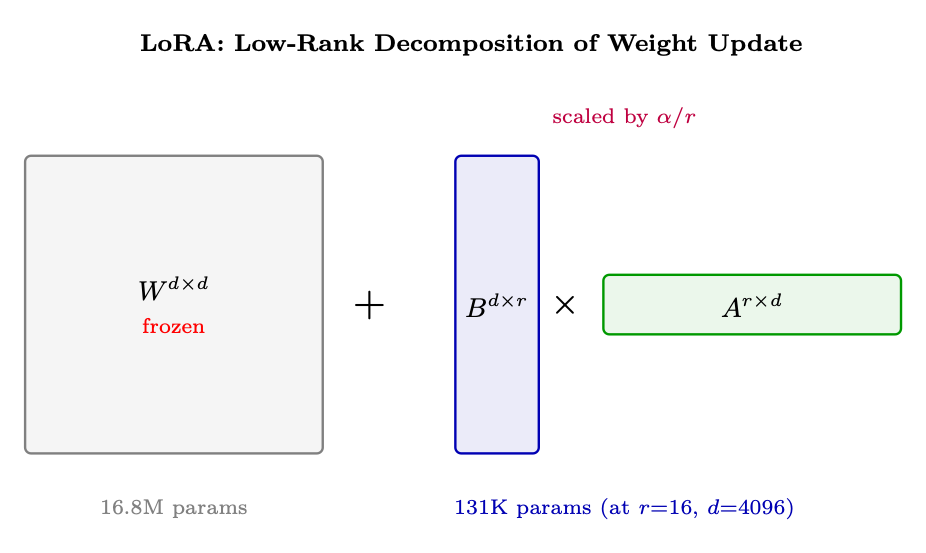
\includegraphics[width=0.85\textwidth]{figures/fig_011_lora-decomposition.png}
% \caption{LoRA decomposes the weight update $\Delta W$ into two small matrices $B \times A$. The original weight $W$ remains frozen; only $B$ and $A$ receive gradients. At inference, the product $BA$ can be merged into $W$ with zero overhead.}
\caption{LoRA 将权重更新 $\Delta W$ 分解为两个小矩阵 $B \times A$。原始权重 $W$ 保持冻结；只有 $B$ 和 $A$ 接收梯度。推理时，乘积 $BA$ 可以零开销地合并到 $W$ 中。}
\label{fig:lora-decomposition}
\end{figure}

% \begin{intuitionbox}[Why the $\alpha/r$ Scaling Matters]
% Without scaling, doubling the rank $r$ would roughly double the magnitude of $\Delta W = BA$ (more columns in $B$ contribute to the sum). This means changing rank would also change how much the model is perturbed---you'd need to re-tune the learning rate every time you adjust $r$.
\begin{intuitionbox}[为什么 $\alpha/r$ 缩放很重要]
如果不做缩放，将秩 $r$ 翻倍大约会让 $\Delta W = BA$ 的幅度翻倍（$B$ 中更多列参与求和）。这意味着改变秩也会改变模型被扰动的幅度——你每次调整 $r$ 都得重新调学习率。

% The $\alpha/r$ factor \textbf{normalizes the update magnitude} so that it stays approximately constant regardless of rank:
$\alpha/r$ 因子\textbf{对更新幅度进行归一化}，使其无论秩为多少都大致保持恒定：
\[
W' = W + \frac{\alpha}{r} \cdot BA
\]

\begin{itemize}
  % \item \textbf{Fix $\alpha$, sweep $r$}: The effective update magnitude stays $\sim\alpha$ regardless of rank. You can try $r \in \{8, 16, 32, 64\}$ without re-tuning LR.
  \item \textbf{固定 $\alpha$，扫描 $r$}：有效更新幅度无论秩为何都保持在 $\sim\alpha$ 附近。可以尝试 $r \in \{8, 16, 32, 64\}$ 而无需重新调学习率。
  % \item \textbf{Common practice}: Set $\alpha = r$ (so $\alpha/r = 1$) or $\alpha = 2r$ (so $\alpha/r = 2$). This is a convenient default where the scaling factor is a small integer.
  \item \textbf{常见做法}：设 $\alpha = r$（即 $\alpha/r = 1$）或 $\alpha = 2r$（即 $\alpha/r = 2$）。这是缩放因子为小整数的便捷默认。
  % \item \textbf{Why not just tune LR?} You could, but $\alpha/r$ provides a \emph{rank-independent} knob. Teams can share LR recipes across experiments with different ranks.
  \item \textbf{为什么不直接调 LR？} 可以，但 $\alpha/r$ 提供了一个\emph{与秩无关}的旋钮。团队可以在不同秩的实验间共享 LR 配方。
  % \item \textbf{rsLoRA insight}~\cite{kalajdzievski2023rslora}: At high ranks ($r \geq 64$), empirical evidence shows $\alpha/\sqrt{r}$ is more stable than $\alpha/r$, because the variance of $BA$ scales with $\sqrt{r}$, not $r$.
  \item \textbf{rsLoRA 洞察}~\cite{kalajdzievski2023rslora}：在高秩（$r \geq 64$）下，经验证据表明 $\alpha/\sqrt{r}$ 比 $\alpha/r$ 更稳定，因为 $BA$ 的方差按 $\sqrt{r}$ 而非 $r$ 缩放。
\end{itemize}
\end{intuitionbox}

\subsection{LoRA 超参数}
\label{lora-hyperparameters}

% Choosing LoRA hyperparameters correctly is critical --- the wrong rank or alpha can either under-fit (too constrained) or waste memory (too expressive).
正确选择 LoRA 超参数至关重要——错误的秩或 alpha 要么欠拟合（约束过强），要么浪费内存（表达力过剩）。

\begin{table}[ht!]
\centering\small
% \caption{LoRA hyperparameter guide.}
\caption{LoRA 超参数指南。}
\noindent\begin{tabularx}{\linewidth}{@{}l Z{0.65} Z{1.35}@{}}
\toprule
\textbf{超参数} & \textbf{典型值} & \textbf{建议} \\
\midrule
% \texttt{r} (rank) & 8, 16, 32, 64 & Higher = more capacity but more memory. Start with 16. \\
\texttt{r}（秩） & 8, 16, 32, 64 & 更高 = 更大容量但更多内存。从 16 开始。 \\
% \texttt{lora\_alpha} & 16, 32 (often $= r$ or $2r$) & Controls update magnitude via $\alpha/r$ scaling. \\
\texttt{lora\_alpha} & 16, 32（通常 $= r$ 或 $2r$） & 通过 $\alpha/r$ 缩放控制更新幅度。 \\
% \texttt{target\_modules} & \texttt{q\_proj, k\_proj, v\_proj, o\_proj} & All attention projections. Add \texttt{gate\_proj, up\_proj, down\_proj} for full coverage. \\
\texttt{target\_modules} & \texttt{q\_proj, k\_proj, v\_proj, o\_proj} & 所有 Attention 投影。添加 \texttt{gate\_proj, up\_proj, down\_proj} 以实现完整覆盖。 \\
% \texttt{lora\_dropout} & 0.0--0.1 & Regularization. Usually 0.05 for small datasets. \\
\texttt{lora\_dropout} & 0.0--0.1 & 正则化。小数据集通常用 0.05。 \\
% \texttt{bias} & \texttt{"none"} & Training biases adds minimal params but rarely helps. \\
\texttt{bias} & \texttt{"none"} & 训练偏置项新增参数极少但很少有帮助。 \\
% Learning rate & $1\text{e-}4$ to $3\text{e-}4$ & Higher than full fine-tuning (only adapters update). \\
学习率 & $1\text{e-}4$ 到 $3\text{e-}4$ & 高于全量微调（只更新适配器）。 \\
\bottomrule
\end{tabularx}
\end{table}

% \begin{warningbox}[Rank Selection Rules of Thumb]
\begin{warningbox}[秩选择经验法则]
\begin{itemize}
  % \item \textbf{r=8}: Simple tasks (single-domain chat, classification). Very memory-efficient.
  \item \textbf{r=8}：简单任务（单领域聊天、分类）。非常省内存。
  % \item \textbf{r=16}: General-purpose fine-tuning. Good default.
  \item \textbf{r=16}：通用微调。良好的默认值。
  % \item \textbf{r=32--64}: Complex tasks (math, code, multi-turn reasoning). Approaches full fine-tune quality.
  \item \textbf{r=32--64}：复杂任务（数学、代码、多轮推理）。接近全量微调质量。
  % \item \textbf{r=128+}: Diminishing returns; consider full fine-tuning or QLoRA with higher rank.
  \item \textbf{r=128+}：收益递减；考虑全量微调或更高秩的 QLoRA。
  % \item \textbf{Key indicator}: If training loss plateaus well above full fine-tune loss, increase rank.
  \item \textbf{关键指标}：若训练损失明显高于全量微调损失而停滞不前，则增大秩。
\end{itemize}
\end{warningbox}

\subsection{LoRA 变体}
\label{lora-variants}

\begin{table}[ht!]
\centering\small
% \caption{LoRA variants and their innovations.}
\caption{LoRA 变体及其创新。}
\noindent\begin{tabularx}{\linewidth}{@{}l Z{1.32} Z{0.68}@{}}
\toprule
\textbf{方法} & \textbf{关键创新} & \textbf{适用场景} \\
\midrule
% \textbf{QLoRA}~\cite{dettmers2023qlora} & 4-bit quantized base + LoRA in BF16. NF4 data type + double quantization. & Fine-tune 70B on single 48GB GPU. \\
\textbf{QLoRA}~\cite{dettmers2023qlora} & 4-bit 量化基座 + BF16 的 LoRA。NF4 数据类型 + 双重量化。 & 在单张 48GB GPU 上微调 70B。 \\
% \textbf{DoRA}~\cite{liu2024dora} & Decomposes $W$ into magnitude and direction; LoRA updates direction only. & Better generalization for reasoning. \\
\textbf{DoRA}~\cite{liu2024dora} & 将 $W$ 分解为幅度与方向；LoRA 只更新方向。 & 推理任务的泛化更好。 \\
% \textbf{LoRA+}~\cite{hayou2024loraplus} & Different LRs for $A$/$B$ ($\eta_B = \lambda \eta_A$, $\lambda \approx 16$). & Free 2\% gain; no extra cost. \\
\textbf{LoRA+}~\cite{hayou2024loraplus} & 为 $A$/$B$ 使用不同的 LR。 & 免费的 2\% 提升；无额外成本。 \\
% \textbf{AdaLoRA}~\cite{zhang2023adalora} & Dynamic rank budget across layers (SVD-based importance). & Very tight compute budget. \\
\textbf{AdaLoRA}~\cite{zhang2023adalora} & 跨层动态秩预算（基于 SVD 的重要性）。 & 算力预算非常紧张时。 \\
% \textbf{rsLoRA}~\cite{kalajdzievski2023rslora} & Scales by $\alpha/\sqrt{r}$ instead of $\alpha/r$. Stable at high ranks. & When using $r \geq 64$. \\
\textbf{rsLoRA}~\cite{kalajdzievski2023rslora} & 用 $\alpha/\sqrt{r}$ 而非 $\alpha/r$ 缩放。在高秩下稳定。 & 使用 $r \geq 64$ 时。 \\
% \textbf{VeRA}~\cite{kopiczko2024vera} & Shared frozen random $A, B$; trains diagonal scaling only. & Extreme param efficiency. \\
\textbf{VeRA}~\cite{kopiczko2024vera} & 共享冻结的随机 $A, B$；只训练对角缩放。 & 极致的参数效率。 \\
% \textbf{LoRA-FA} & Freezes $A$ after init; only trains $B$. Halves LoRA memory. & Memory-constrained scenarios. \\
\textbf{LoRA-FA} & 初始化后冻结 $A$；只训练 $B$。将 LoRA 内存减半。 & 内存受限场景。 \\
\bottomrule
\end{tabularx}
\end{table}

\subsubsection{关键扩展详解}
\label{key-extensions-explained}

% \paragraph{DoRA -- Weight-Decomposed Low-Rank Adaptation.}
\paragraph{DoRA——权重分解低秩适配（Weight-Decomposed Low-Rank Adaptation，DoRA）。}
\label{dora-weight-decomposed-low-rank-adaptation.}

% DoRA~\cite{liu2024dora} observes that full fine-tuning tends to change the \emph{direction} of weight vectors more than their magnitude. Standard LoRA conflates both. DoRA decomposes each weight column into magnitude $m = \|W\|_\text{col}$ and direction $\hat{V} = W / \|W\|_\text{col}$, then applies LoRA only to the direction:
DoRA~\cite{liu2024dora}观察到，全量微调倾向于改变权重向量的\emph{方向}多于幅度。标准 LoRA 把二者混在一起。DoRA 将每个权重列分解为幅度 $m = \|W\|_\text{col}$ 和方向 $\hat{V} = W / \|W\|_\text{col}$，然后只对方向应用 LoRA：
\[
W' = m \odot \hat{V}', \quad \hat{V}' = \frac{W + BA}{\|W + BA\|_\text{col}}
\]
% Magnitude $m$ is a separate learnable vector (one scalar per column). This consistently outperforms LoRA by 1--3\% on reasoning and instruction-following benchmarks with no additional inference cost (merged at deployment).
幅度 $m$ 是单独的可学习向量（每列一个标量）。它在推理与指令遵循基准上始终比 LoRA 高 1--3\%，且无额外推理成本（部署时合并）。

\newpage
% \paragraph{LoRA+ -- Asymmetric Learning Rates.}
\paragraph{LoRA+——非对称学习率。}
\label{lora-asymmetric-learning-rates.}

% Hayou et al.~\cite{hayou2024loraplus} show that matrices $A$ and $B$ in LoRA have different optimal learning rates. Since $B$ is initialized to zero, it starts in a very different regime than $A$ (initialized from $\mathcal{N}(0, \sigma^2)$). Setting $\eta_B \approx 16 \times \eta_A$ improves convergence speed and final quality by $\sim$2\% --- a free gain requiring only a one-line config change:
Hayou 等~\cite{hayou2024loraplus}表明，LoRA 中的矩阵 $A$ 和 $B$ 拥有不同的最优学习率。由于 $B$ 初始化为零，它与从 $\mathcal{N}(0, \sigma^2)$ 初始化的 $A$ 处于截然不同的状态。设置 $\eta_B \approx 16 \times \eta_A$ 可提升收敛速度并将最终质量提高约 2\%——一个仅需一行配置改动的免费收益：

\begin{lstlisting}[style=pythonstyle]
# PEFT 中的 LoRA+：为每个矩阵设置不同的学习率
optimizer_grouped_parameters = [
    {"params": [p for n, p in model.named_parameters() if "lora_B" in n],
     "lr": 2e-4 * 16},   # B 矩阵：更高的学习率
    {"params": [p for n, p in model.named_parameters() if "lora_A" in n],
     "lr": 2e-4},         # A 矩阵：基础学习率
]
\end{lstlisting}

% \paragraph{VeRA -- Vector-based Random Matrix Adaptation.}
\paragraph{VeRA——基于向量的随机矩阵适配（Vector-based Random Matrix Adaptation，VeRA）。}
\label{vera-vector-based-random-matrix-adaptation.}

% VeRA~\cite{kopiczko2024vera} takes parameter efficiency to the extreme: instead of learning $A$ and $B$, it \emph{freezes} them as shared random matrices across all layers and only trains two diagonal scaling vectors $d_b \in \mathbb{R}^r$ and $d_a \in \mathbb{R}^d$:
VeRA~\cite{kopiczko2024vera}把参数效率推向极致：它不学习 $A$ 和 $B$，而是将它们\emph{冻结}为所有层之间共享的随机矩阵，仅训练两个对角缩放向量 $d_b \in \mathbb{R}^r$ 和 $d_a \in \mathbb{R}^d$：
\[
\Delta W = B \cdot \text{diag}(d_b) \cdot A \cdot \text{diag}(d_a)
\]
% This reduces trainable parameters by $\sim$10$\times$ vs.~LoRA (only $r + d$ params per layer) while achieving 90--95\% of LoRA quality. Best for scenarios where you need hundreds of task-specific adapters with minimal storage.
这相比 LoRA 将可训练参数减少约 10$\times$（每层只有 $r + d$ 个参数），同时达到 LoRA 90--95\% 的质量。最适合需要数百个任务专用适配器、且存储极小化的场景。

% \begin{examplebox}[QLoRA Memory Savings]
% \textbf{70B model full fine-tune}: 140 GB (weights) + 280 GB (optimizer) + 140 GB (gradients) = 560 GB (7$\times$ A100-80GB).
\begin{examplebox}[QLoRA 内存节省]
\textbf{70B 模型全量微调}：140 GB（权重） + 280 GB（优化器） + 140 GB（梯度） = 560 GB（7$\times$ A100-80GB）。

% \textbf{70B QLoRA (r=16, all linear layers)}:
\textbf{70B QLoRA（r=16，所有线性层）}：

\begin{itemize}
  % \item Base model in NF4: $70\text{B} \times 0.5 = 35$ GB
  \item NF4 格式的基座模型：$70\text{B} \times 0.5 = 35$ GB
  % \item LoRA adapters in BF16: $\sim$160 MB
  \item BF16 格式的 LoRA 适配器：$\sim$160 MB
  % \item Optimizer states (only for adapters): $\sim$320 MB
  \item 优化器状态（仅适配器）：$\sim$320 MB
  % \item Activations (gradient checkpointing): $\sim$8 GB
  \item 激活值（梯度检查点）：$\sim$8 GB
  % \item \textbf{Total: $\sim$44 GB} --- fits in a single 48GB GPU!
  \item \textbf{总计：$\sim$44 GB}——可装入单张 48GB GPU！
\end{itemize}
\end{examplebox}

\begin{lstlisting}[style=pythonstyle]
# 使用 PEFT 的 QLoRA 配置
from peft import LoraConfig, get_peft_model, prepare_model_for_kbit_training
from transformers import BitsAndBytesConfig
import torch

# 4-bit 量化配置
bnb_config = BitsAndBytesConfig(
    load_in_4bit=True,
    bnb_4bit_quant_type="nf4",           # NormalFloat4 - 对权重最优
    bnb_4bit_compute_dtype=torch.bfloat16, # 计算使用 BF16
    bnb_4bit_use_double_quant=True,       # 对量化常数再次量化
)

# LoRA 配置
lora_config = LoraConfig(
    r=16,
    lora_alpha=32,                        # alpha/r = 2 倍缩放
    target_modules=["q_proj", "k_proj", "v_proj", "o_proj",
                    "gate_proj", "up_proj", "down_proj"],
    lora_dropout=0.05,
    bias="none",
    task_type="CAUSAL_LM",
)

model = prepare_model_for_kbit_training(model)  # 为 QLoRA 做准备
model = get_peft_model(model, lora_config)       # 添加 LoRA 适配器
model.print_trainable_parameters()
# 输出：trainable params: 83,886,080 || all params: 70,553,706,496 || 0.12%
\end{lstlisting}

\subsection{其他 PEFT 方法}
\label{other-peft-approaches}

% LoRA dominates modern practice, but it is not the only parameter-efficient method. For completeness, the main alternatives:
LoRA 主导了现代实践，但并非唯一的参数高效方法。为完整起见，列出主要的替代方案：

\begin{table}[ht!]
\centering\small
% \caption{PEFT method families. LoRA is the de facto standard for LLM fine-tuning; the others are included for historical context and niche use cases.}
\caption{参数高效微调（Parameter-Efficient Fine-Tuning，PEFT）方法家族。LoRA 是 LLM 微调的事实标准；其余方法列在此处用于历史背景和小众使用场景。}
\noindent\begin{tabularx}{\linewidth}{@{}l Z{1.21} Z{1.51} Z{0.3}@{}}
\toprule
\textbf{方法} & \textbf{机制} & \textbf{优点 / 缺点} & \textbf{现状} \\
\midrule
% \textbf{LoRA}~\cite{hu2021lora} (and variants) & Low-rank matrices added to existing weights & Mergeable at inference (zero overhead); well-supported; works for all architectures & \textbf{Standard} \\
\textbf{LoRA}~\cite{hu2021lora}（及变体） & 在现有权重上添加低秩矩阵 & 推理时可合并（零开销）；支持完善；适用于所有架构 & \textbf{标准} \\
% \textbf{Adapters}~\cite{houlsby2019adapters} & Small bottleneck MLPs inserted between layers & Modular; stackable; adds inference latency (extra sequential layers) & Rarely used \\
\textbf{Adapters}~\cite{houlsby2019adapters} & 在层之间插入小型瓶颈 MLP & 模块化；可堆叠；增加推理延迟（额外的串行层） & 很少使用 \\
% \textbf{Prefix Tuning}~\cite{li2021prefix} & Learnable ``virtual tokens'' prepended to keys/values at each layer & No weight modification; effective for generation tasks; consumes context length & Niche \\
\textbf{前缀微调}~\cite{li2021prefix} & 在每层 K/V 前拼接可学习的「虚拟 Token」 & 不修改权重；对生成任务有效；占用上下文长度 & 小众 \\
% \textbf{Prompt Tuning}~\cite{lester2021prompt} & Learnable soft prompt embeddings prepended to input & Extremely few params ($<$0.01\%); weaker than LoRA for complex tasks & Niche \\
\textbf{提示微调}~\cite{lester2021prompt} & 在输入前拼接可学习的软提示 Embedding & 参数极少（$<$0.01\%）；复杂任务上弱于 LoRA & 小众 \\
% \textbf{IA3}~\cite{liu2022ia3} & Learned vectors that rescale keys, values, and FFN activations & Even fewer params than LoRA; mergeable; limited capacity & Deprecated \\
\textbf{IA3}~\cite{liu2022ia3} & 用学到的向量对 K、V 和 FFN 激活进行重缩放 & 参数比 LoRA 更少；可合并；容量有限 & 已弃用 \\
% \textbf{BitFit}~\cite{zaken2022bitfit} & Train only bias terms & Near-zero params; surprisingly effective for simple tasks; limited expressiveness & Historical \\
\textbf{BitFit}~\cite{zaken2022bitfit} & 只训练偏置项 & 参数接近于零；在简单任务上意外有效；表达力有限 & 历史方法 \\
\bottomrule
\end{tabularx}
\end{table}

% \begin{intuitionbox}[Why LoRA Won]
% LoRA became the standard because it uniquely combines: (1)~\textbf{zero inference overhead} --- adapters merge into base weights, unlike Adapters or Prefix Tuning which add latency or consume context; (2)~\textbf{composability} --- multiple LoRA adapters can be swapped at serving time for multi-tenant deployments; (3)~\textbf{ecosystem support} --- HuggingFace PEFT, TRL, vLLM, and all major frameworks have first-class LoRA support; (4)~\textbf{proven at scale} --- used in production by Meta, Google, and most open-source fine-tunes on HuggingFace. Unless you have a specific constraint that LoRA cannot satisfy, it should be your default choice.
\begin{intuitionbox}[为什么 LoRA 胜出]
LoRA 成为标准是因为它独特地兼具：(1)~\textbf{零推理开销}——适配器可合并入基座权重，不像 Adapters 或前缀微调会增加延迟或消耗上下文；(2)~\textbf{可组合性}——多个 LoRA 适配器可在服务时切换，用于多租户部署；(3)~\textbf{生态支持}——HuggingFace PEFT、TRL、vLLM 以及所有主流框架都对 LoRA 有一等支持；(4)~\textbf{大规模验证}——Meta、Google 以及 HuggingFace 上大多数开源微调都在生产中使用。除非你有 LoRA 无法满足的特定约束，否则它应当是你的默认选择。
\end{intuitionbox}

\clearpage
\section{专家混合模型（Mixture of Experts，MoE）}
\label{mixture-of-experts-moe}

% Mixture of Experts models~\cite{shazeer2017outrageously, jiang2024mixtral} scale model capacity without proportionally scaling compute cost by activating only a subset of parameters for each token.
专家混合模型~\cite{shazeer2017outrageously, jiang2024mixtral} 通过对每个 Token 只激活参数的一个子集，从而在不按比例增加计算成本的情况下扩展模型容量。

\subsection{架构}
\label{architecture}

\begin{keybox}[MoE 层]
% In a MoE transformer, the FFN layer in each block is replaced by $N$ parallel ``expert'' FFNs plus a \textbf{router} that selects which experts to use:
在一个 MoE Transformer 中，每个块中的 FFN 层被替换为 $N$ 个并行的“专家” FFN，再加上一个 \textbf{路由器（router）} 来选择使用哪些专家：
\[
\text{MoE}(x) = \sum_{i=1}^{N} g_i(x) \cdot E_i(x), \quad g(x) = \text{TopK}(\text{softmax}(W_r x))
\]

\begin{itemize}
  % \item $E_i$ are expert networks (standard FFN layers)
  \item $E_i$ 是专家网络（标准的 FFN 层）
  % \item $g_i(x)$ are gating weights from the router (only top-$K$ are non-zero)
  \item $g_i(x)$ 是来自路由器的门控权重（只有 top-$K$ 个非零）
  % \item Typically $K=2$ out of $N=8$--64 experts are active per token
  \item 通常每个 Token 在 $N=8$--64 个专家中激活 $K=2$ 个
  % \item Total params scale with $N$; \textbf{active params} scale with $K/N$ of FFN size
  \item 总参数量随 $N$ 增长；\textbf{激活参数量} 按 FFN 大小的 $K/N$ 比例增长
\end{itemize}
\end{keybox}

\begin{figure}[ht!]
\centering
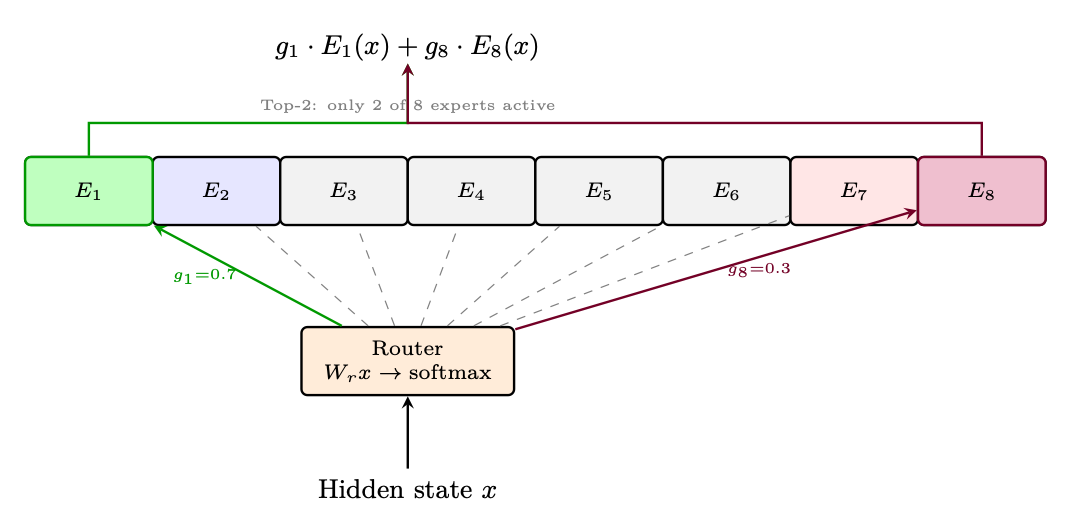
\includegraphics[width=0.85\textwidth]{figures/fig_012_fig12.png}
% \caption{MoE layer with 8 experts and Top-2 routing. Only the two highest-gated experts are computed per token; the rest are skipped entirely.}
\caption{具有 8 个专家和 Top-2 路由的 MoE 层。每个 Token 只计算门控值最高的两个专家；其余专家被完全跳过。}
\end{figure}

\subsection{负载均衡}
\label{load-balancing}

\begin{warningbox}[负载均衡问题]
% Without constraints, the router may send most tokens to the same 1--2 experts (``expert collapse''). This wastes capacity and creates compute imbalance across GPUs (each expert typically lives on a different GPU).
在没有约束的情况下，路由器可能会把大多数 Token 都发送到相同的 1--2 个专家上（“专家坍缩（expert collapse）”）。这既浪费了容量，又造成了跨 GPU 的计算不均衡（每个专家通常位于不同的 GPU 上）。

% \textbf{Solution}: Add an auxiliary load-balancing loss:
\textbf{解决方案}：添加一个辅助的负载均衡损失：
\[
\mathcal{L}_{\text{bal}} = \alpha \cdot N \sum_{i=1}^{N} f_i \cdot p_i
\]
% where $f_i$ = fraction of tokens routed to expert $i$, $p_i$ = mean router probability for expert $i$. This encourages uniform expert utilization.
其中 $f_i$ 表示路由到专家 $i$ 的 Token 比例，$p_i$ 表示专家 $i$ 的平均路由概率。这鼓励了对专家的均匀利用。
\end{warningbox}

\subsection{噪声 Top-K 门控（Noisy Top-K Gating）：让离散路由变得可训练}
\label{noisy-top-k-gating-making-discrete-routing-trainable}

% The core challenge in MoE is that \textbf{top-$k$ selection is not differentiable} --- you can't backpropagate through a hard ``pick the top 2'' operation. The field has developed two key tricks to solve this:
MoE 的核心挑战在于 \textbf{top-$k$ 选择是不可微的}——你无法通过一个硬性的“挑选前 2 名”操作反向传播。该领域发展出了两个关键技巧来解决这个问题：

\begin{intuitionbox}[路由可微性问题]
% The router computes logits $h(x) = W_r \cdot x$ for each expert, then selects the top-$k$. But:
路由器为每个专家计算 logits $h(x) = W_r \cdot x$，然后选择 top-$k$。但是：

\begin{itemize}
  % \item The \emph{selected} experts get gradients through their gate weights (softmax over selected)
  \item \emph{被选中} 的专家会通过其门控权重获得梯度（在被选中者上做 softmax）
  % \item The \emph{selection decision itself} (which $k$ to pick) has zero gradient
  \item \emph{选择决策本身}（挑选哪 $k$ 个）的梯度为零
  % \item Without a trick, the router can get stuck: an expert never selected $\rightarrow$ never gets a gradient signal $\rightarrow$ never gets selected
  \item 如果没有技巧，路由器可能会卡住：一个从未被选中的专家 $\rightarrow$ 永远得不到梯度信号 $\rightarrow$ 永远不会被选中
\end{itemize}
\end{intuitionbox}

% \paragraph{Approach 1: Noisy Top-K Gating~\cite{shazeer2017outrageously}.}
\paragraph{方法 1：噪声 Top-K 门控（Noisy Top-K Gating）~\cite{shazeer2017outrageously}。}
\label{approach-1-noisy-top-k-gating-.}

% Add learnable Gaussian noise to the router logits \emph{before} the top-$k$ selection:
在进行 top-$k$ 选择 \emph{之前}，向路由器的 logits 添加可学习的高斯噪声：

\begin{align}
  h(x) &= W_g \cdot x \tag{clean logits} \\
  H(x) &= h(x) + \epsilon \cdot \text{Softplus}(W_{\text{noise}} \cdot x), \quad \epsilon \sim \mathcal{N}(0, 1) \tag{noisy logits} \\
  \text{TopK}(v, k)_i &= \begin{cases} v_i & \text{if } v_i \text{ is in the top } k \\ -\infty & \text{otherwise} \end{cases} \\
  g(x) &= \text{softmax}\big(\text{TopK}(H(x),\, k)\big) \tag{sparse gates}
\end{align}

\begin{itemize}
  % \item $W_{\text{noise}}$ is a \emph{learned} noise magnitude --- the model learns how much exploration each expert needs
  \item $W_{\text{noise}}$ 是 \emph{学习得到的} 噪声幅度——模型会学习每个专家需要多少探索量
  % \item During training, noise occasionally promotes ``underdog'' experts into the top-$k$, giving them gradient signal
  \item 在训练过程中，噪声偶尔会将“弱势”专家提升到 top-$k$ 中，使其获得梯度信号
  % \item At inference, noise is removed: use clean logits $h(x)$ for deterministic routing
  \item 在推理时去除噪声：使用干净的 logits $h(x)$ 进行确定性路由
  % \item The Softplus ensures noise scale is always positive
  \item Softplus 确保噪声尺度始终为正
\end{itemize}

% \paragraph{Approach 2: Gumbel-Softmax Trick (for differentiable discrete sampling).}
\paragraph{方法 2：Gumbel-Softmax 技巧（Gumbel-Softmax Trick，用于可微的离散采样）。}
\label{approach-2-gumbel-softmax-trick-for-differentiable-discrete-sampling.}

% An alternative from the variational inference literature~\cite{jang2017categorical}. The \textbf{Gumbel-Max trick} provides exact sampling from a categorical distribution:
来自变分推断文献的另一种方法~\cite{jang2017categorical}。\textbf{Gumbel-Max 技巧（Gumbel-Max trick）} 提供了从类别分布中精确采样的方式：

\begin{equation}
  z = \arg\max_i \left[ \log \pi_i + G_i \right], \quad G_i \sim \text{Gumbel}(0,1)
\end{equation}

% where Gumbel noise is generated as $G_i = -\log(-\log(U_i)),\; U_i \sim \text{Uniform}(0,1)$.
其中 Gumbel 噪声由 $G_i = -\log(-\log(U_i)),\; U_i \sim \text{Uniform}(0,1)$ 生成。

% For \textbf{top-$k$ routing}: taking the top-$k$ of $(\log \pi_i + G_i)$ gives $k$ samples \emph{without replacement} from the categorical distribution defined by $\pi$.
对于 \textbf{top-$k$ 路由}：取 $(\log \pi_i + G_i)$ 的 top-$k$，等价于从由 $\pi$ 定义的类别分布中 \emph{无放回地} 抽取 $k$ 个样本。

% Since $\arg\max$ is non-differentiable, the \textbf{Gumbel-Softmax} relaxation replaces it with a temperature-controlled softmax:
由于 $\arg\max$ 是不可微的，\textbf{Gumbel-Softmax} 松弛将其替换为一个由温度控制的 softmax：

\begin{equation}
  \hat{g}_i = \frac{\exp\left((\log \pi_i + G_i) / \tau\right)}{\sum_j \exp\left((\log \pi_j + G_j) / \tau\right)}
\end{equation}

\begin{itemize}
  % \item $\tau \to 0$: approaches a hard one-hot (exact but non-differentiable)
  \item $\tau \to 0$：趋近于硬 one-hot（精确但不可微）
  % \item $\tau \to \infty$: approaches uniform (differentiable but uninformative)
  \item $\tau \to \infty$：趋近于均匀分布（可微但无信息量）
  % \item In practice, anneal $\tau$ from 1.0 down to 0.1--0.5 during training
  \item 实践中，在训练过程中将 $\tau$ 从 1.0 退火到 0.1--0.5
  % \item \textbf{Straight-through estimator}: use hard top-$k$ in the forward pass, but Gumbel-Softmax gradients in the backward pass --- best of both worlds
  \item \textbf{直通估计器（Straight-through estimator）}：前向传播中使用硬 top-$k$，反向传播中使用 Gumbel-Softmax 梯度——两全其美
\end{itemize}

\begin{keybox}[实际中使用的是哪种方法？]
\begin{itemize}
  % \item \textbf{Sparsely-Gated MoE~\cite{shazeer2017outrageously}, Mixtral~\cite{jiang2024mixtral}, DeepSeek-V2~\cite{deepseekv2}}: Use Noisy Top-K with Gaussian noise. Simple, effective, well-proven at scale.
  \item \textbf{Sparsely-Gated MoE~\cite{shazeer2017outrageously}、Mixtral~\cite{jiang2024mixtral}、DeepSeek-V2~\cite{deepseekv2}}：使用带高斯噪声的噪声 Top-K。简单、有效，在大规模上得到了充分验证。
  % \item \textbf{Switch Transformer~\cite{fedus2022switch}}: Simplified to Top-1 with no noise (relies on load-balancing loss alone).
  \item \textbf{Switch Transformer~\cite{fedus2022switch}}：简化为不带噪声的 Top-1（仅依赖负载均衡损失）。
  % \item \textbf{Research / smaller-scale MoE}: Some use Gumbel-Softmax for fully differentiable routing, especially when learning the routing itself is the research objective.
  \item \textbf{研究型 / 小规模 MoE}：一些工作使用 Gumbel-Softmax 实现完全可微的路由，尤其是当学习路由本身就是研究目标时。
  % \item \textbf{Key insight}: Both approaches solve the same problem (making discrete selection trainable) via noise injection. Gaussian noise is simpler; Gumbel noise has stronger theoretical guarantees for categorical sampling.
  \item \textbf{关键见解}：两种方法都通过噪声注入解决了同一个问题（让离散选择可训练）。高斯噪声更简单；Gumbel 噪声在类别采样上有更强的理论保证。
\end{itemize}
\end{keybox}

\subsection{值得关注的 MoE 模型}
\label{notable-moe-models}

\noindent\begin{tabularx}{\linewidth}{@{}l Z{0.47} Z{0.47} Z{0.62} Z{2.44}@{}}
\toprule
\textbf{模型} & \textbf{总参数量} & \textbf{激活参数量} & \textbf{专家} & \textbf{创新点} \\
\midrule
Switch Transformer~\cite{fedus2022switch} & 1.6T & 100B & 128, Top-1 & 首个大规模 MoE；简化的路由 \\
Mixtral 8x7B~\cite{jiang2024mixtral} & 47B & 13B & 8, Top-2 & 开放权重；质量媲美 Llama-2 70B \\
DeepSeek-V2~\cite{deepseekv2} & 236B & 21B & 160, Top-6 & 带共享 + 路由专家的 DeepSeekMoE \\
Qwen-MoE~\cite{qwen2024qwen25} & 14.3B & 2.7B & 60, Top-4 & 为提升效率而设计的细粒度专家 \\
DBRX~\cite{databricks2024dbrx} & 132B & 36B & 16, Top-4 & 每块 4 个专家的细粒度结构 \\
\bottomrule
\end{tabularx}

\section{LLM 训练中的多样性}
\label{diversity-in-llm-training}

% Diversity --- in training data, model outputs, and optimization trajectories --- is critical for preventing mode collapse and ensuring robust, general-purpose LLMs. This section covers the key diversity mechanisms applicable to all LLM training phases.
多样性——在训练数据、模型输出和优化轨迹上的多样性——对于防止模式坍缩并确保鲁棒的通用 LLM 至关重要。本节介绍适用于所有 LLM 训练阶段的关键多样性机制。

\subsection{采样多样性}
\label{sampling-diversity}

\begin{keybox}[用于多样化生成的采样策略]
\begin{itemize}
  % \item \textbf{Temperature $\tau$}: $P(x_i) \propto \exp(\text{logit}_i / \tau)$. Higher $\tau$ = more uniform distribution = more diverse. Typical: $\tau=0.7$--$1.0$ for RLHF generation.
  \item \textbf{温度 $\tau$}：$P(x_i) \propto \exp(\text{logit}_i / \tau)$。更高的 $\tau$ = 更均匀的分布 = 更多样化。典型值：RLHF 生成中使用 $\tau=0.7$--$1.0$。
  % \item \textbf{Top-$k$}: Only sample from the $k$ highest-probability tokens. Prevents degenerate low-probability tokens.
  \item \textbf{Top-$k$}：只从概率最高的 $k$ 个 Token 中采样。防止退化的低概率 Token。
  % \item \textbf{Top-$p$ (nucleus)}: Sample from the smallest set of tokens whose cumulative probability $\geq p$. Adaptive: more diverse when the model is uncertain.
  \item \textbf{Top-$p$（核采样，Nucleus Sampling）}：从累计概率 $\geq p$ 的最小 Token 集合中采样。自适应：模型不确定时更多样。
  % \item \textbf{Min-$p$}: Only keep tokens with $P \geq p_{\min} \times P_{\max}$. More principled than top-$k$.
  \item \textbf{Min-$p$}：仅保留满足 $P \geq p_{\min} \times P_{\max}$ 的 Token。比 top-$k$ 更具原理性。
  % \item \textbf{Frequency/presence penalty}: Penalize tokens that appeared in the response. Encourages lexical diversity.
  \item \textbf{频率/出现惩罚（Frequency/presence penalty）}：对已在回复中出现过的 Token 进行惩罚。鼓励词汇多样性。
\end{itemize}
\end{keybox}

\subsection{训练数据多样性}
\label{training-data-diversity}

\begin{itemize}
  % \item \textbf{Prompt diversity}: Cover different domains, difficulty levels, and formats. The Goldilocks principle: prompts should have 20--80\% success rate.
  \item \textbf{提示多样性}：覆盖不同的领域、难度等级和格式。Goldilocks 原则：提示的成功率应在 20--80\% 之间。
  % \item \textbf{Deduplication}: Remove near-duplicate training examples (MinHash, n-gram overlap). Duplicates cause overfitting to specific patterns.
  \item \textbf{去重}：移除近似重复的训练样本（MinHash、n-gram 重叠）。重复样本会导致对特定模式的过拟合。
  % \item \textbf{Data mixing}: Balance across tasks/domains using temperature-weighted sampling or curriculum strategies.
  \item \textbf{数据混合}：使用温度加权采样或课程策略，在任务/领域之间进行平衡。
\end{itemize}

\subsection{促进多样性的方法}
\label{diversity-promoting-methods}

\noindent\begin{tabularx}{\linewidth}{@{}l Z{1}@{}}
\toprule
\textbf{方法} & \textbf{它如何促进多样性} \\
\midrule
温度缩放（Temperature scaling） & 更高的 $\tau$ 会让分布变得更平坦；更多 Token 变得合理。 \\
Top-$p$ / Min-$p$ & 自适应阈值允许模型在不确定时进行更广的采样。 \\
频率惩罚（Frequency penalty） & 惩罚重复出现的 Token，强制在一次回复内产生词汇多样性。 \\
数据去重 & 从训练数据中移除近似重复样本，防止对特定模式的过拟合。 \\
多领域混合 & 跨领域的温度加权采样确保了广泛的覆盖。 \\
口头化采样（Verbalized sampling） & 提示模型显式地用语言表达出对回复的概率分布~\cite{zhang2025verbalized}。见 §\ref{grpo-variants-and-extensions}。 \\
\bottomrule
\end{tabularx}

\section{文本生成：解码方法}
\label{text-generation-decoding-methods}

% A trained language model outputs a probability distribution over the vocabulary at each step: $P(x_t | x_{<t})$. The \textbf{decoding strategy} determines how we select the next token from this distribution. This choice profoundly affects output quality, diversity, and coherence.
一个训练好的语言模型在每一步都会输出一个在词表上的概率分布：$P(x_t | x_{<t})$。\textbf{解码策略} 决定了我们如何从该分布中选择下一个 Token。这个选择深刻地影响输出质量、多样性和连贯性。

\subsection{贪心解码（Greedy Decoding）}
\label{greedy-decoding}

% The simplest strategy: always pick the highest-probability token.
最简单的策略：总是选择概率最高的 Token。
\[
x_t = \arg\max_{v \in \mathcal{V}} P(v | x_{<t})
\]

% \textbf{Intuition:} Like always taking the most obvious next word in a sentence. ``The capital of France is...'' $\to$ ``Paris'' (probability 0.92).
\textbf{直觉：} 就像在句子中总是选取最显而易见的下一个词。"The capital of France is..." $\to$ "Paris"（概率 0.92）。

% \textbf{Pros:} Deterministic, fast, no hyperparameters.\\
\textbf{优点：} 确定性、快速、无超参数。\\

% \textbf{Cons:} Produces repetitive, generic text. Misses high-quality sequences where an early low-probability token leads to a globally better output. No diversity.
\textbf{缺点：} 产生重复、泛泛的文本。当一个早期的低概率 Token 会带来全局更优输出时会被错过。没有多样性。

\subsection{束搜索（Beam Search）}
\label{beam-search}

% Maintain $B$ (beam width) partial hypotheses in parallel, expanding each by the top-$k$ tokens and keeping the $B$ highest-scoring complete sequences:
并行维护 $B$ 个（束宽）部分假设，每一步用 top-$k$ 个 Token 扩展每个假设，并保留得分最高的 $B$ 个完整序列：
\[
\text{score}(y_{1:t}) = \sum_{i=1}^{t} \log P(y_i | y_{<i})
\]
% With \textbf{length normalization} to avoid favoring short sequences:
配合 \textbf{长度归一化（length normalization）} 避免偏好短序列：
\[
\text{score}_{\text{norm}}(y) = \frac{1}{|y|^\alpha} \sum_{i=1}^{|y|} \log P(y_i | y_{<i}), \quad \alpha \in [0.6, 1.0]
\]

% \textbf{Intuition:} Like exploring multiple paths in a maze simultaneously, keeping only the $B$ most promising ones at each junction.
\textbf{直觉：} 就像同时在迷宫中探索多条路径，并在每个岔路口只保留 $B$ 条最有希望的路径。

% \textbf{Pros:} Finds higher-likelihood sequences than greedy; good for translation and summarization where there's a single ``correct'' output.\\
\textbf{优点：} 能找到比贪心解码似然更高的序列；适合翻译和摘要等存在单一“正确”输出的任务。\\

% \textbf{Cons:} Still tends toward generic, repetitive text for open-ended generation; $B \times$ more compute; all beams often converge to similar outputs.
\textbf{缺点：} 对开放式生成仍倾向于产生泛泛、重复的文本；计算量增加 $B$ 倍；所有束往往收敛到相似的输出。

\begin{figure}[ht!]
\centering
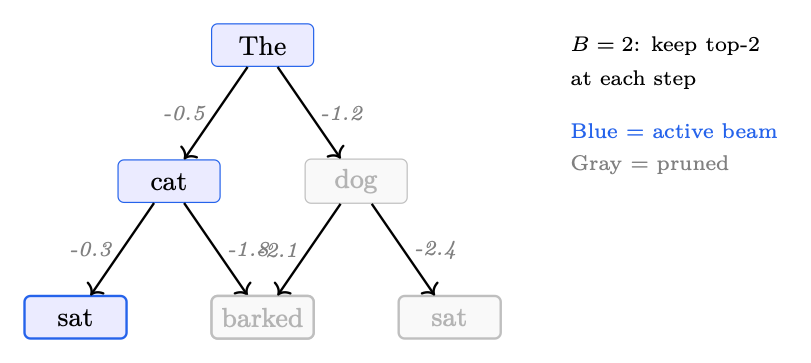
\includegraphics[width=0.7\textwidth]{figures/fig_013_fig13.png}
% \caption{Beam search with $B=2$. At each step, only the 2 highest-scoring partial sequences survive (blue). Lower-scoring alternatives are pruned (gray).}
\caption{束宽为 $B=2$ 的束搜索。在每一步，只有得分最高的 2 个部分序列会被保留（蓝色）。得分较低的候选会被剪枝（灰色）。}
\end{figure}

\subsection{多样化束搜索（Diverse Beam Search）}
\label{diverse-beam-search}

% Standard beam search produces near-duplicate beams. Diverse beam search~\cite{vijayakumar2018diverse} partitions beams into $G$ groups and adds a \textbf{dissimilarity penalty} between groups:
标准束搜索会产生近似重复的束。多样化束搜索（Diverse Beam Search）~\cite{vijayakumar2018diverse} 将束划分为 $G$ 个组，并在组之间添加一个 \textbf{不相似性惩罚（dissimilarity penalty）}：
\[
\text{score}_g(y_t) = \log P(y_t | y_{<t}) - \lambda \sum_{g'<g} \Delta(y_t, Y_{g'})
\]
% where $\Delta$ measures overlap (e.g., Hamming diversity) with tokens already selected by earlier groups, and $\lambda$ controls diversity strength.
其中 $\Delta$ 衡量与较早组已选 Token 的重叠（例如 Hamming 多样性），$\lambda$ 控制多样性强度。

% \textbf{Intuition:} Like forcing a brainstorming group to generate different ideas --- each subgroup is penalized for repeating what earlier subgroups said.
\textbf{直觉：} 就像强迫一个头脑风暴小组生成不同的想法——每个子组若重复了较早子组所说的内容就会被惩罚。

% \textbf{Pros:} Produces genuinely different candidate sequences; useful for reranking pipelines.\\
\textbf{优点：} 产生真正不同的候选序列；对重排序流水线很有用。\\

% \textbf{Cons:} Diversity penalty can degrade individual beam quality; more hyperparameters ($G$, $\lambda$).
\textbf{缺点：} 多样性惩罚可能降低单个束的质量；超参数更多（$G$、$\lambda$）。

\subsection{\texorpdfstring{Top-$k$ 采样}{Top-k Sampling}}
\label{top-k-sampling}

% Sample from only the $k$ most probable tokens, redistributing probability mass:
仅从概率最高的 $k$ 个 Token 中采样，并重新分配概率质量：
\[
P'(v | x_{<t}) = \begin{cases}
    \dfrac{P(v | x_{<t})}{\sum_{v' \in \text{Top-}k} P(v' | x_{<t})} & \text{if } v \in \text{Top-}k \\[6pt]
    0 & \text{otherwise}
  \end{cases}
\]

% \textbf{Intuition:} After ``The cat sat on the...'', only consider the top $k$ plausible continuations (``mat'', ``floor'', ``couch'', ...) and ignore extremely unlikely ones (``quantum'', ``archipelago'').
\textbf{直觉：} 在 "The cat sat on the..." 之后，只考虑前 $k$ 个合理的延续（"mat"、"floor"、"couch"……），忽略那些极不可能的（"quantum"、"archipelago"）。

% \textbf{Pros:} Removes tail noise; simple to implement.\\
\textbf{优点：} 去除尾部噪声；实现简单。\\

% \textbf{Cons:} Fixed $k$ is too restrictive for peaked distributions (wastes probability mass) and too permissive for flat distributions (lets in garbage tokens).
\textbf{缺点：} 固定的 $k$ 对尖峰分布而言过于严格（浪费概率质量），对平坦分布而言又过于宽松（让垃圾 Token 进入）。

\subsection{\texorpdfstring{Top-$p$ 采样（核采样，Nucleus Sampling）}{Top-p (Nucleus) Sampling}}
\label{top-p-nucleus-sampling}

% Sample from the smallest set of tokens whose cumulative probability exceeds $p$:
从累计概率超过 $p$ 的最小 Token 集合中采样：
\[
\text{Top-}p = \min \left\{ S \subseteq \mathcal{V} : \sum_{v \in S} P(v | x_{<t}) \geq p \right\}
\]
% where tokens are sorted by descending probability and added until the threshold $p$ is reached.
其中 Token 按概率降序排序，并逐个加入直到达到阈值 $p$。

% \textbf{Intuition:} Adaptively resize the candidate pool. If the model is confident (``Paris'' at 95\%), the nucleus is tiny. If uncertain (``The movie was...''), the nucleus expands to include many plausible adjectives.
\textbf{直觉：} 自适应地调整候选池大小。如果模型很自信（"Paris" 概率 95\%），核就很小。如果不确定（"The movie was..."），核会扩展以包含许多合理的形容词。

% \textbf{Pros:} Adapts to distribution shape; widely used default ($p=0.9$--$0.95$).\\
\textbf{优点：} 能适应分布形状；广泛使用的默认设置（$p=0.9$--$0.95$）。\\

% \textbf{Cons:} Still includes some low-quality tokens at the tail of the nucleus; the threshold is a single global hyperparameter.
\textbf{缺点：} 在核的尾部仍会包含一些低质量 Token；阈值是一个单一的全局超参数。

\begin{figure}[ht!]
\centering
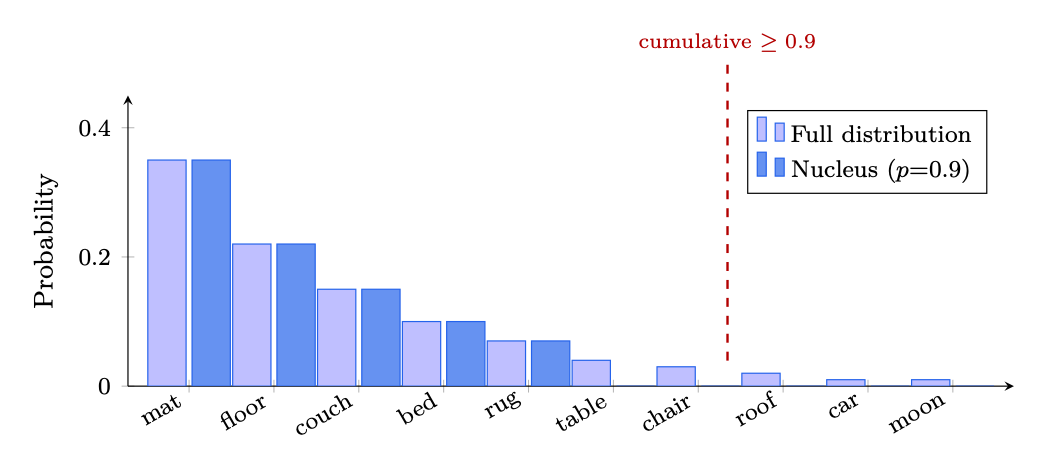
\includegraphics[width=0.85\textwidth]{figures/fig_014_fig14.png}
% \caption{Top-$p$ (nucleus) sampling: tokens are sorted by probability and included until cumulative mass reaches $p=0.9$. The nucleus (dark blue) adapts its size to the distribution shape --- here 5 tokens suffice.}
\caption{Top-$p$（核）采样：Token 按概率排序并依次加入，直到累计质量达到 $p=0.9$。核（深蓝）会根据分布形状自适应其大小——这里 5 个 Token 就足够了。}
\end{figure}

\begin{intuitionbox}[Top-$k$ 与 Top-$p$]
% Consider predicting the next word:
考虑预测下一个词：

\begin{itemize}
  % \item After ``2 + 2 ='': distribution is peaked --- top-1 token (``4'') has 99\% mass. Top-$k$=50 wastefully considers 49 wrong answers. Top-$p$=0.9 correctly picks just ``4''.
  \item 在 "2 + 2 =" 之后：分布是尖峰的——top-1 Token（"4"）占据 99\% 的质量。Top-$k$=50 会浪费地考虑 49 个错误答案。Top-$p$=0.9 则正确地只选取 "4"。
  % \item After ``I enjoy eating'': distribution is flat --- many foods are plausible. Top-$k$=5 is too restrictive. Top-$p$=0.9 might include 50+ tokens, matching the actual uncertainty.
  \item 在 "I enjoy eating" 之后：分布是平坦的——许多食物都合理。Top-$k$=5 太过严格。Top-$p$=0.9 可能会包含 50 多个 Token，与实际的不确定性相匹配。
\end{itemize}

% Top-$p$ adapts; top-$k$ doesn't. In practice, both are often combined: sample from top-$p$ intersected with top-$k$.
Top-$p$ 自适应；top-$k$ 不会。实践中，两者常被结合使用：从 top-$p$ 与 top-$k$ 的交集中采样。
\end{intuitionbox}

\subsection{\texorpdfstring{Min-$p$ 采样}{Min-p Sampling}}
\label{min-p-sampling}

% A recent alternative that sets a \textbf{relative} probability floor~\cite{nguyen2024minp}:
一种较新的替代方法，它设置一个 \textbf{相对} 概率下限~\cite{nguyen2024minp}：
\[
\text{Min-}p = \left\{ v \in \mathcal{V} : P(v | x_{<t}) \geq p_{\min} \cdot \max_{v'} P(v' | x_{<t}) \right\}
\]
% Only tokens with probability at least $p_{\min}$ times the top token's probability are kept.
只有概率至少为最高 Token 概率 $p_{\min}$ 倍的 Token 才会被保留。

% \textbf{Intuition:} ``Only consider tokens that are at least 10\% as likely as the best token.'' If the top token has probability 0.8, only tokens above 0.08 survive. If the top token has probability 0.05 (very uncertain), tokens above 0.005 survive --- naturally expanding the pool.
\textbf{直觉：} “只考虑那些其可能性至少为最优 Token 10\% 的 Token。” 如果最高 Token 的概率为 0.8，那么只有概率高于 0.08 的 Token 能留下。如果最高 Token 的概率为 0.05（非常不确定），概率高于 0.005 的 Token 都能留下——自然地扩大了候选池。

% \textbf{Pros:} Scales naturally with model confidence; fewer degenerate samples than top-$p$ on peaked distributions; single intuitive parameter.\\
\textbf{优点：} 会随模型置信度自然伸缩；在尖峰分布上比 top-$p$ 产生更少的退化样本；只有一个直观的参数。\\

% \textbf{Cons:} Newer, less battle-tested; not yet standard in all inference frameworks.
\textbf{缺点：} 较新、经受的实战检验较少；尚未在所有推理框架中成为标准。

\subsection{温度缩放}
\label{temperature-scaling}

% Before applying any sampling strategy, logits are divided by temperature $T$:
在应用任何采样策略之前，将 logits 除以温度 $T$：
\[
P_T(v | x_{<t}) = \frac{\exp(z_v / T)}{\sum_{v'} \exp(z_{v'} / T)}
\]

\begin{itemize}
  % \item $T < 1$: Sharpens distribution $\to$ more deterministic, focused outputs.
  \item $T < 1$：使分布更尖锐 $\to$ 更确定、更聚焦的输出。
  % \item $T = 1$: Unmodified model distribution.
  \item $T = 1$：未修改的模型分布。
  % \item $T > 1$: Flattens distribution $\to$ more random, creative outputs.
  \item $T > 1$：使分布更平坦 $\to$ 更随机、更有创造性的输出。
  % \item $T \to 0$: Becomes greedy decoding. $T \to \infty$: Becomes uniform sampling.
  \item $T \to 0$：退化为贪心解码。$T \to \infty$：退化为均匀采样。
\end{itemize}

% \textbf{Common settings:} $T=0.7$ for factual tasks, $T=1.0$--$1.2$ for creative writing, $T=0.0$ (greedy) for code/math.
\textbf{常见设置：} 事实性任务 $T=0.7$，创意写作 $T=1.0$--$1.2$，代码/数学 $T=0.0$（贪心）。

\subsection{对比解码（Contrastive Decoding）}
\label{contrastive-decoding}

% Contrastive decoding~\cite{li2023contrastive} exploits the difference between a strong model (expert) and a weak model (amateur) to amplify the expert's unique knowledge:
对比解码（Contrastive Decoding）~\cite{li2023contrastive} 利用一个强模型（专家）与一个弱模型（业余者）之间的差异，来放大专家独有的知识：
\[
x_t = \arg\max_{v \in \mathcal{V}(x_{<t})} \left[ \log P_{\text{expert}}(v | x_{<t}) - \log P_{\text{amateur}}(v | x_{<t}) \right]
\]
% where $\mathcal{V}(x_{<t}) = \{v : P_{\text{expert}}(v | x_{<t}) \geq \alpha \cdot \max_{v'} P_{\text{expert}}(v' | x_{<t})\}$ is an adaptive plausibility constraint.
其中 $\mathcal{V}(x_{<t}) = \{v : P_{\text{expert}}(v | x_{<t}) \geq \alpha \cdot \max_{v'} P_{\text{expert}}(v' | x_{<t})\}$ 是一个自适应的合理性约束。

% \textbf{Intuition:} The amateur model captures generic, obvious patterns (common words, repetition). Subtracting its log-probabilities removes this ``generic signal,'' leaving the expert's distinctive knowledge and reasoning. Like removing background noise from a recording to hear the signal.
\textbf{直觉：} 业余模型捕捉到的是泛泛的、显而易见的模式（常用词、重复）。减去其对数概率就去除了这种“泛泛信号”，留下专家独有的知识和推理。就像从录音中去除背景噪声以听见信号一样。

% \textbf{Pros:} Reduces repetition and generic phrasing; improves factuality and coherence without additional training; works with any model pair.\\
\textbf{优点：} 减少重复和泛泛的措辞；在不额外训练的情况下提升事实性和连贯性；可与任意一对模型搭配使用。\\

% \textbf{Cons:} Requires running two models (2$\times$ compute); sensitive to amateur model choice; the plausibility threshold $\alpha$ needs tuning.
\textbf{缺点：} 需要运行两个模型（计算量加倍）；对业余模型的选择敏感；合理性阈值 $\alpha$ 需要调优。

\subsection{重复惩罚}
\label{repetition-penalties}

% Orthogonal to the sampling strategy, repetition penalties discourage the model from repeating tokens. Given the raw logit $z_v$ for token $v$ (i.e., the unnormalized score output by the LM head \emph{before} softmax), the penalized logit is:
与采样策略正交，重复惩罚（repetition penalties）阻止模型重复 Token。给定 Token $v$ 的原始 logit $z_v$（即 LM 头在 softmax \emph{之前} 输出的未归一化得分），惩罚后的 logit 为：
\[
z_v' = \begin{cases}
    z_v / \theta & \text{if } v \in \text{generated tokens and } z_v > 0 \\
    z_v \cdot \theta & \text{if } v \in \text{generated tokens and } z_v < 0
  \end{cases}
\]
% where $\theta > 1$ is the penalty factor (typically 1.1--1.3). In both cases, the effect is to push the logit toward zero---reducing the probability of previously generated tokens. Frequency and presence penalties are simpler additive variants used by OpenAI APIs:
其中 $\theta > 1$ 是惩罚因子（通常为 1.1--1.3）。在两种情况下，其效果都是把 logit 推向零——从而降低先前生成 Token 的概率。频率惩罚和出现惩罚是 OpenAI API 使用的更简单的加性变体：
\[
z_v' = z_v - \alpha \cdot \text{count}(v) - \beta \cdot \mathbf{1}[v \in \text{generated}]
\]
% where $\alpha$ is the frequency penalty (proportional to how many times $v$ appeared) and $\beta$ is the presence penalty (flat penalty for any prior occurrence).
其中 $\alpha$ 是频率惩罚（与 $v$ 出现次数成正比），$\beta$ 是出现惩罚（对任何先前出现给予恒定惩罚）。

\subsection{实际对比}
\label{practical-comparison}

\begin{table}[ht!]
\centering\small
% \caption{Decoding method comparison for LLM text generation.}
\caption{LLM 文本生成中各解码方法的对比。}
\begin{tabularx}{0.88\linewidth}{@{}l Z{0.64} Z{0.64} Z{0.64} Z{2.08}@{}}
\toprule
\textbf{方法} & \textbf{是否确定性} & \textbf{多样性} & \textbf{质量} & \textbf{最佳适用} \\
\midrule
Greedy & 是 & 无 & 中等 & 代码、事实问答 \\
Beam Search（$B$=4--8） & 是 & 低 & 高（较窄） & 翻译、摘要 \\
Diverse Beam Search & 是 & 中等 & 高 & 用于重排序的候选生成 \\
Top-$k$（$k$=50） & 否 & 中等 & 中等 & 通用生成 \\
Top-$p$（$p$=0.9） & 否 & 自适应 & 高 & 开放式任务的默认选择 \\
Min-$p$（$p_{\min}$=0.1） & 否 & 自适应 & 高 & top-$p$ 的稳健替代 \\
Contrastive & 是 & 低 & 非常高 & 事实性、连贯的长文本 \\
\bottomrule
\end{tabularx}
\end{table}

\begin{examplebox}[实际中的解码：``Once upon a time'']
% Given the prompt ``Once upon a time,'':
给定提示 "Once upon a time,"：

\begin{itemize}
  % \item \textbf{Greedy}: ``there was a young girl who lived in a small village...'' (generic fairy tale)
  \item \textbf{Greedy}: "there was a young girl who lived in a small village..."（泛泛的童话）
  % \item \textbf{Top-$p$=0.9, $T$=1.0}: ``the rivers ran backwards and the fish learned to fly...'' (creative, surprising)
  \item \textbf{Top-$p$=0.9, $T$=1.0}: "the rivers ran backwards and the fish learned to fly..."（有创意、出人意料）
  % \item \textbf{Top-$p$=0.9, $T$=0.3}: ``there was a kingdom ruled by a wise and just king...'' (coherent, conventional)
  \item \textbf{Top-$p$=0.9, $T$=0.3}: "there was a kingdom ruled by a wise and just king..."（连贯、常规）
  % \item \textbf{Contrastive}: ``in the amber-lit corridors of a collapsing star, two minds argued about the nature of time...'' (distinctive, avoids clichés)
  \item \textbf{Contrastive}: "in the amber-lit corridors of a collapsing star, two minds argued about the nature of time..."（独特，避免了陈词滥调）
\end{itemize}

% Same model, same prompt --- decoding strategy determines the character of the output.
同一个模型、同一个提示——解码策略决定了输出的风格。
\end{examplebox}

\subsection{受限解码（Constrained Decoding，结构化生成 Structured Generation）}
\label{sec:constrained-decoding}

% All methods above sample from the \emph{full} vocabulary at each step. \textbf{Constrained decoding} restricts the set of allowed tokens so that the output is \emph{guaranteed} to conform to a formal grammar---typically a JSON schema, regex, or context-free grammar (CFG).
上述所有方法都在每一步从 \emph{完整的} 词表中采样。\textbf{受限解码（Constrained Decoding）} 限制允许的 Token 集合，从而 \emph{保证} 输出符合某种形式语法——通常是 JSON 模式、正则表达式或上下文无关文法（Context-Free Grammar，CFG）。

\paragraph{核心机制。}
\label{core-mechanism.}

% At each decoding step $t$, a \textbf{token mask} $M_t \subseteq \mathcal{V}$ is computed from the current parser state. Only tokens in $M_t$ receive their original logits; all others are set to $-\infty$ before softmax:
在每个解码步 $t$，会根据当前解析器状态计算一个 \textbf{Token 掩码（token mask）} $M_t \subseteq \mathcal{V}$。只有 $M_t$ 中的 Token 保留其原始 logits；在 softmax 之前，所有其它 Token 都被设为 $-\infty$：
\[
P'(v | x_{<t}) = \begin{cases}
    P(v | x_{<t}) / Z & \text{if } v \in M_t \\
    0 & \text{otherwise}
  \end{cases}
\]
% where $Z = \sum_{v \in M_t} P(v | x_{<t})$ renormalizes. Because the mask changes every step (it depends on what has been generated so far), the constraint is enforced \emph{incrementally}---the model cannot produce an invalid prefix at any point.
其中 $Z = \sum_{v \in M_t} P(v | x_{<t})$ 用于重新归一化。由于掩码每一步都会变化（它取决于到目前为止已经生成的内容），约束是 \emph{逐步} 强制实施的——模型在任何位置都不可能生成一个非法前缀。

\paragraph{从模式到掩码。}
\label{from-schema-to-mask.}

% The compilation pipeline is:
编译流水线为：
\[
\text{JSON Schema} \;\xrightarrow{\text{compile}}\; \text{Regex}
  \;\xrightarrow{\text{compile}}\; \text{FSM (DFA)}
  \;\xrightarrow{\text{index}}\; \text{Token Mask per State}
\]
% The FSM states correspond to positions in the regex. For each state, all vocabulary tokens that would keep the string in the language are precomputed into an index (a one-time cost per schema). At runtime, looking up the mask is an $O(1)$ table access---adding negligible latency to each decoding step.
有限状态机（FSM）的状态对应正则表达式中的位置。对每个状态，所有能使字符串保持在该语言内的词表 Token 都被预计算成索引（对每个模式只需一次性的开销）。在运行时，查询掩码只是一次 $O(1)$ 的表访问——对每个解码步带来的延迟可忽略不计。

\paragraph{关键库。}
\label{key-libraries.}

\begin{itemize}
  % \item \textbf{Outlines}~\cite{willard2023outlines}: Compiles JSON schemas and regexes into interleaved FSM-guided generation. Supports any model with a logits interface.
  \item \textbf{Outlines}~\cite{willard2023outlines}：将 JSON 模式和正则表达式编译为交织的、由 FSM 引导的生成。支持任何提供 logits 接口的模型。
  % \item \textbf{lm-format-enforcer}\footnote{\url{https://github.com/noamgat/lm-format-enforcer}}: Similar FSM approach with a focus on integration with serving frameworks (vLLM, TGI).
  \item \textbf{lm-format-enforcer}\footnote{\url{https://github.com/noamgat/lm-format-enforcer}}：类似的 FSM 方法，重点放在与服务框架（vLLM、TGI）的集成上。
  % \item \textbf{Guidance}\footnote{\url{https://github.com/guidance-ai/guidance}} (Microsoft): Interleaves constrained generation with control flow (loops, conditions), enabling complex structured outputs beyond flat schemas.
  \item \textbf{Guidance}\footnote{\url{https://github.com/guidance-ai/guidance}}（Microsoft）：将受限生成与控制流（循环、条件）交织在一起，可实现超越扁平模式的复杂结构化输出。
  % \item \textbf{XGrammar}~\cite{dong2024xgrammar}: Pushdown-automaton-based engine supporting full context-free grammars (not just regular languages), used in MLC-LLM and vLLM for grammar-mode decoding.
  \item \textbf{XGrammar}~\cite{dong2024xgrammar}：基于下推自动机的引擎，支持完整的上下文无关文法（不仅限于正则语言），被 MLC-LLM 和 vLLM 用于语法模式的解码。
\end{itemize}

\paragraph{权衡。}
\label{trade-offs.}

% Constrained decoding \emph{guarantees} syntactic validity---no post-hoc parsing failures, no retries. However:
受限解码 \emph{保证} 了语法有效性——不会出现事后解析失败，也无需重试。然而：

\begin{itemize}
  % \item \textbf{Semantic quality}: Forcing structure can degrade content quality if the model's probability mass for the ``correct'' answer lies outside the grammar. In practice this is rare for well-trained models on well-designed schemas.
  \item \textbf{语义质量}：如果模型对“正确”答案的概率质量位于语法之外，强制结构可能会降低内容质量。在实践中，对于设计良好的模式和训练良好的模型，这种情况很少出现。
  % \item \textbf{Compilation cost}: The FSM index must be built per schema. For complex schemas this can take 1--5 s, but it is amortized over all requests using that schema.
  \item \textbf{编译开销}：必须为每个模式构建 FSM 索引。对于复杂模式可能需要 1--5 秒，但这一开销会在所有使用该模式的请求间摊销。
  % \item \textbf{Grammar coverage}: Regex/FSM handles JSON, YAML, SQL fragments, and most structured formats. Full CFGs (via XGrammar or LALR parsers) cover languages like Python or XML.
  \item \textbf{语法覆盖}：正则/FSM 可处理 JSON、YAML、SQL 片段以及大多数结构化格式。完整的 CFG（通过 XGrammar 或 LALR 解析器）可覆盖 Python 或 XML 等语言。
\end{itemize}

\begin{keybox}[何时使用受限解码]
% Use constrained decoding whenever the consumer of the model's output is a program rather than a human. Tool-calling agents, API backends, and data-extraction pipelines all benefit from \emph{guaranteed} valid structure. For free-form prose or creative text, unconstrained sampling remains appropriate.
当模型输出的消费者是程序而不是人类时，就应使用受限解码。工具调用智能体、API 后端和数据抽取流水线都能从 \emph{有保证的} 合法结构中受益。对于自由形式的散文或创意文本，无约束采样仍然是合适的选择。
\end{keybox}

% \section{Prompt Engineering}
\section{Prompt 工程}
\label{sec:prompt-engineering}

% Prompt engineering is the discipline of designing inputs to LLMs that reliably elicit desired behaviour---without changing model weights. While fine-tuning modifies the model, prompt engineering exploits the model's \emph{existing} capabilities through careful framing, examples, and structure. It is the fastest, cheapest, and most accessible lever for improving LLM outputs, and remains essential even when using fine-tuned models.
Prompt 工程是一门设计 LLM 输入的学科，目标是在不修改模型权重的情况下可靠地激发预期行为。微调修改的是模型本身，而 Prompt 工程则通过精心的框架、示例与结构来挖掘模型\emph{已有}的能力。它是改善 LLM 输出最快、最便宜、也最易获得的杠杆，即使在使用微调模型时也依然不可或缺。

% \subsection{In-Context Learning (ICL)}
\subsection{上下文学习（In-Context Learning，ICL）}
\label{in-context-learning-icl}

% In-context learning~\cite{brown2020language} is the remarkable ability of large language models to learn tasks at inference time purely from examples provided in the prompt---with no gradient updates. The model implicitly infers the task from the pattern of input--output pairs and generalizes to new inputs.
上下文学习~\cite{brown2020language} 是大语言模型一项令人瞩目的能力：在推理时仅凭 Prompt 中提供的示例就能学习任务，完全无需梯度更新。模型从输入-输出对的模式中隐式推断任务，并泛化到新的输入上。

\begin{keybox}[为什么上下文学习有效]
\begin{itemize}
  % \item \textbf{Implicit Bayesian inference}: The model has seen millions of tasks during pretraining. The prompt examples \emph{locate} the relevant task in the model's learned distribution~\cite{xie2022explanation}.
  \item \textbf{隐式贝叶斯推断}：模型在预训练时见过数百万种任务。Prompt 示例在模型学到的分布中\emph{定位}到相关任务~\cite{xie2022explanation}。
  % \item \textbf{Induction heads}: Specific attention heads learn to copy patterns (``A is to B as C is to ''), enabling in-context generalization~\cite{olsson2022context}.
  \item \textbf{归纳头（Induction heads）}：特定的 attention 头学会复制模式（``A 之于 B，如 C 之于 ''），从而实现上下文泛化~\cite{olsson2022context}。
  % \item \textbf{Task vectors}: ICL creates implicit task representations in the residual stream that steer generation toward the demonstrated format and content~\cite{todd2024function}.
  \item \textbf{任务向量（Task vectors）}：ICL 在残差流中创建隐式的任务表示，引导生成朝向所演示的格式与内容~\cite{todd2024function}。
\end{itemize}
\end{keybox}

% \paragraph{Scaling behaviour.}
\paragraph{扩展行为。}
\label{scaling-behaviour.}

% ICL emerges primarily in models above $\sim$1B parameters and improves log-linearly with model scale~\cite{brown2020language}. Smaller models can memorize examples but struggle to generalize to novel inputs within the same context window.
ICL 主要在参数量约 1B 以上的模型中涌现，并随模型规模呈对数线性提升~\cite{brown2020language}。较小的模型可以记住示例，但难以在同一上下文窗口内泛化到新的输入。

% \subsection{Zero-Shot Prompting}
\subsection{零样本提示（Zero-Shot Prompting）}
\label{zero-shot-prompting}

% Zero-shot prompting provides \emph{no} examples---only a task description or instruction. The model must rely entirely on its pretrained knowledge and instruction-tuning to produce the correct format and content.
零样本提示\emph{不}提供任何示例，只有任务描述或指令。模型必须完全依靠预训练知识与指令微调来生成正确的格式与内容。

\begin{examplebox}[零样本分类]
\begin{lstlisting}
Classify the following movie review as POSITIVE or NEGATIVE.

Review: "The cinematography was breathtaking but the plot
felt rushed and predictable."

Sentiment:
\end{lstlisting}
\end{examplebox}

% \paragraph{When zero-shot works well:}
\paragraph{零样本何时奏效：}
\label{when-zero-shot-works-well}

\begin{itemize}
  % \item Tasks the model has seen extensively during pretraining/SFT (translation, summarization, sentiment)
  \item 模型在预训练/SFT 阶段大量见过的任务（翻译、摘要、情感分析）
  % \item Well-specified instructions with unambiguous output format
  \item 指令明确、输出格式无歧义
  % \item Instruction-tuned models (e.g., ChatGPT, Claude, Llama-3-Instruct) significantly outperform base models at zero-shot tasks~\cite{ouyang2022training}
  \item 指令微调模型（如 ChatGPT、Claude、Llama-3-Instruct）在零样本任务上显著优于基座模型~\cite{ouyang2022training}
\end{itemize}

% \paragraph{When zero-shot fails:}
\paragraph{零样本何时失效：}
\label{when-zero-shot-fails}

% Novel formats, domain-specific labeling schemes, or ambiguous tasks where the model cannot infer your exact requirements from the instruction alone.
全新格式、领域特定的标注方案，或模型无法仅凭指令推断出确切需求的模糊任务。

% \subsection{Few-Shot Prompting}
\subsection{少样本提示（Few-Shot Prompting）}
\label{few-shot-prompting}

% Few-shot prompting~\cite{brown2020language} provides $k$ input--output examples (``shots'') before the actual query. This is the most common form of in-context learning and remains one of the most effective prompting strategies.
少样本提示~\cite{brown2020language} 在实际查询之前提供 $k$ 个输入-输出示例（即 ``shots''）。它是上下文学习最常见的形式，也仍然是最有效的提示策略之一。

\begin{examplebox}[少样本命名实体识别]
\begin{lstlisting}
Extract named entities from the text. Format: [ENTITY](TYPE)

Text: "Apple released the iPhone 15 in Cupertino."
Entities: [Apple](ORG), [iPhone 15](PRODUCT), [Cupertino](LOC)

Text: "Elon Musk announced Tesla's new factory in Berlin."
Entities: [Elon Musk](PER), [Tesla](ORG), [Berlin](LOC)

Text: "OpenAI partnered with Microsoft to deploy GPT-4."
Entities:
\end{lstlisting}
\end{examplebox}

% \paragraph{Key design principles for few-shot examples:}
\paragraph{少样本示例的关键设计原则：}
\label{key-design-principles-for-few-shot-examples}

\begin{enumerate}
  % \item \textbf{Diversity}: Cover the range of expected inputs (different lengths, edge cases, categories).
  \item \textbf{多样性}：覆盖预期输入的范围（不同长度、边界情况、类别）。
  % \item \textbf{Ordering}: Place harder or more representative examples last (recency bias)~\cite{lu2022fantastically}.
  \item \textbf{顺序}：将较难或更具代表性的示例放在最后（近因偏差，recency bias）~\cite{lu2022fantastically}。
  % \item \textbf{Label balance}: If classifying, include examples from all classes to avoid majority-class bias.
  \item \textbf{标签平衡}：分类任务中要包含所有类别的示例，以避免多数类偏差。
  % \item \textbf{Format consistency}: Every example must follow the \emph{exact} same structure. The model mimics the pattern.
  \item \textbf{格式一致性}：每个示例都必须遵循\emph{完全}相同的结构。模型会模仿这种模式。
  % \item \textbf{Relevance}: Use examples semantically similar to the target query for best results~\cite{liu2022makes}.
  \item \textbf{相关性}：选用与目标查询语义相近的示例可获得最佳效果~\cite{liu2022makes}。
\end{enumerate}

% \paragraph{How many shots?}
\paragraph{需要多少个示例？}
\label{how-many-shots}

% Performance typically improves from 0 to 4--8 examples, then plateaus. Beyond $\sim$20 examples, gains are marginal and you risk filling the context window. Min et al.~\cite{min2022rethinking} showed that the \emph{format} and \emph{label space} of examples matter more than label correctness---even random labels help (though correct labels help more).
性能通常会从 0 个示例提升到 4--8 个示例，然后趋于平稳。超过约 20 个示例后收益微乎其微，反而有占满上下文窗口的风险。Min 等人~\cite{min2022rethinking} 表明，示例的\emph{格式}与\emph{标签空间}比标签正确性更重要——即使随机标签也有帮助（不过正确标签帮助更大）。

% \subsection{Instruction-Following Prompts}
\subsection{指令跟随类 Prompt}
\label{instruction-following-prompts}

% Instruction-tuned models respond best to clear, structured instructions. The key insight: treat the prompt as a \emph{specification}, not a suggestion.
指令微调模型对清晰、结构化的指令响应最好。关键洞察是：把 Prompt 当作\emph{规范说明}，而不是建议。

\begin{keybox}[高效指令型 Prompt 的解剖]
\begin{enumerate}
  % \item \textbf{Role/Persona}: Define who the model is (``You are a senior data scientist...'')
  \item \textbf{角色/人格}：定义模型是谁（``你是一名资深数据科学家……''）
  % \item \textbf{Task}: What to do, stated clearly and unambiguously
  \item \textbf{任务}：要做什么，表述清晰无歧义
  % \item \textbf{Context}: Background information the model needs
  \item \textbf{上下文}：模型需要的背景信息
  % \item \textbf{Constraints}: Length limits, tone, what to avoid, output format
  \item \textbf{约束}：长度限制、语气、需要避免的内容、输出格式
  % \item \textbf{Examples} (optional): Show the desired output format
  \item \textbf{示例}（可选）：展示期望的输出格式
  % \item \textbf{Input}: The actual data to process
  \item \textbf{输入}：实际待处理的数据
\end{enumerate}
\end{keybox}

\begin{examplebox}[带约束的指令型 Prompt]
\begin{lstlisting}
Role: You are a medical literature reviewer.

Task: Summarize the following research abstract for a
general audience.

Constraints:
- Maximum 3 sentences
- No jargon (explain any technical terms)
- Include the key finding and its clinical implication
- Do NOT speculate beyond what the abstract states

Abstract: [...]
\end{lstlisting}
\end{examplebox}

% \paragraph{System prompts vs.~user prompts.}
\paragraph{System Prompt 与 User Prompt 的对比。}
\label{system-prompts-vs.-user-prompts.}

% Modern chat APIs separate the \emph{system} prompt (persistent instructions, role definition) from the \emph{user} message (per-turn input). System prompts are processed with higher attention priority in most models and provide a natural place for role definitions, constraints, and output format specifications~\cite{openai2023gpt4}.
现代聊天 API 将\emph{系统} Prompt（持久指令、角色定义）与\emph{用户}消息（每轮输入）分离。多数模型对 system prompt 赋予更高的 attention 优先级，是放置角色定义、约束和输出格式说明的天然位置~\cite{openai2023gpt4}。

% \subsection{Structured Output Prompts (JSON/XML)}
\subsection{结构化输出 Prompt（JSON/XML）}
\label{structured-output-prompts-jsonxml}

% For programmatic use, the most critical prompting technique is enforcing structured output---particularly JSON.
对于程序化用途，最关键的提示技术是强制结构化输出——尤其是 JSON。

\begin{examplebox}[JSON 输出 Prompt]
\begin{lstlisting}
Extract the following information from the customer email.
Respond ONLY with valid JSON, no other text.

Schema:
{
  "intent": "refund|complaint|question|praise",
  "urgency": "low|medium|high",
  "product_mentioned": "string or null",
  "summary": "one sentence summary"
}

Email: [...]
\end{lstlisting}
\end{examplebox}

% \paragraph{Techniques for reliable structured output:}
\paragraph{获得可靠结构化输出的技巧：}
\label{techniques-for-reliable-structured-output}

\begin{itemize}
  % \item \textbf{Schema-first}: Show the exact JSON schema \emph{before} the input. The model treats it as a template.
  \item \textbf{Schema 优先}：在输入\emph{之前}展示精确的 JSON schema，模型会将其当作模板。
  % \item \textbf{Constrained decoding}: Use grammar-based sampling (e.g., Outlines~\cite{willard2023outlines}, Guidance) to guarantee syntactically valid JSON at the token level.
  \item \textbf{约束解码（Constrained decoding）}：使用基于语法的采样（如 Outlines~\cite{willard2023outlines}、Guidance）在 token 级别保证 JSON 语法合法。
  % \item \textbf{XML tags}: For nested or multi-part outputs, XML tags (e.g., \texttt{<thinking>...</thinking>}) provide unambiguous delimiters that models follow reliably.
  \item \textbf{XML 标签}：对于嵌套或多段输出，XML 标签（如 \texttt{<thinking>...</thinking>}）提供无歧义的分隔符，模型能可靠地遵循。
  % \item \textbf{Pydantic/TypeScript types}: Providing type definitions helps models understand field constraints (OpenAI's function calling uses JSON Schema internally).
  \item \textbf{Pydantic/TypeScript 类型}：提供类型定义有助于模型理解字段约束（OpenAI 的 function calling 内部就使用 JSON Schema）。
\end{itemize}

\begin{warningbox}[Prompt 中的 JSON —— 常见陷阱]
\begin{itemize}
  % \item Models may add markdown fences (\texttt{‘‘‘json ... ‘‘‘}) --- instruct explicitly to output raw JSON.
  \item 模型可能加上 markdown 代码围栏（\texttt{‘‘‘json ... ‘‘‘}）——需明确要求输出原始 JSON。
  % \item Nested objects and arrays increase hallucination risk --- flatten schemas where possible.
  \item 嵌套对象和数组会增加幻觉风险——尽量将 schema 扁平化。
  % \item Enum fields (fixed choices) are much more reliable than free-text fields.
  \item 枚举字段（固定选项）比自由文本字段可靠得多。
  % \item Always validate outputs programmatically; no prompt guarantees 100\% compliance without constrained decoding.
  \item 始终要在程序中校验输出；不借助约束解码，任何 Prompt 都无法 100\% 保证合规。
\end{itemize}
\end{warningbox}

% \paragraph{JSON Prompting: Structuring the Input.}
\paragraph{JSON Prompting：结构化输入本身。}
\label{json-prompting-structuring-the-input.}

% A distinct but complementary technique is \emph{JSON prompting}---formatting the prompt \emph{itself} as JSON rather than natural language. This exploits the model's extensive pre-training on structured data (APIs, configs, code) to improve instruction adherence, reduce ambiguity, and enable deterministic parsing of multi-field requests.
一种独立但互补的技术是 \emph{JSON prompting}——将 Prompt \emph{本身}格式化为 JSON 而非自然语言。这利用了模型在结构化数据（API、配置、代码）上的大量预训练，从而提升指令遵循度、降低歧义，并使多字段请求能被确定性地解析。

\begin{examplebox}[结合 System Prompt 的 JSON Prompting]
\begin{lstlisting}
=== SYSTEM ===
You are a senior code reviewer. Analyze code for bugs,
security issues, and style violations. Always respond
in the JSON schema provided.

=== USER (JSON prompt) ===
{
  "task": "code_review",
  "language": "python",
  "severity_filter": "high",
  "code": "def login(user, pw):\n    query = ...",
  "output_schema": {
    "issues": [{
      "line": "int",
      "severity": "critical|high|medium|low",
      "category": "security|bug|style|performance",
      "description": "string",
      "fix": "string"
    }],
    "overall_risk": "critical|high|medium|low"
  }
}
\end{lstlisting}

% \textbf{Why JSON prompting works:}
\textbf{为何 JSON prompting 有效：}

\begin{itemize}
  % \item \textbf{Unambiguous field boundaries}: No confusion about where one instruction ends and another begins.
  \item \textbf{无歧义的字段边界}：不会混淆一条指令何处结束、下一条何处开始。
  % \item \textbf{Typed constraints}: Fields like \texttt{"severity\_filter": "high"} are clearer than ``only show high severity issues.''
  \item \textbf{带类型的约束}：像 \texttt{"severity\_filter": "high"} 这样的字段比 ``只显示高严重度问题'' 更清晰。
  % \item \textbf{Schema-as-contract}: Including \texttt{output\_schema} in the input mirrors API design patterns the model has seen extensively during pre-training.
  \item \textbf{Schema 即契约}：在输入中加入 \texttt{output\_schema} 复刻了模型在预训练中大量见过的 API 设计模式。
  % \item \textbf{System prompt still essential}: The system message provides \emph{role}, \emph{tone}, and \emph{behavioral constraints} that don't fit naturally in a JSON payload.
  \item \textbf{System prompt 依然不可或缺}：System 消息提供\emph{角色}、\emph{语气}与\emph{行为约束}，这些内容并不适合放进 JSON 负载里。
\end{itemize}
\end{examplebox}

% \subsection{Chain-of-Thought (CoT) Prompting}
\subsection{思维链（Chain-of-Thought，CoT）Prompting}
\label{chain-of-thought-cot-prompting}

% Chain-of-thought prompting~\cite{wei2022chain} asks the model to produce intermediate reasoning steps before giving a final answer. This simple technique dramatically improves performance on tasks requiring multi-step reasoning: arithmetic, logic, commonsense inference, and code generation.
思维链 Prompting~\cite{wei2022chain} 要求模型在给出最终答案之前先生成中间推理步骤。这一简单技术在需要多步推理的任务上（算术、逻辑、常识推断与代码生成）能带来显著的性能提升。

% \paragraph{Why CoT works:}
\paragraph{CoT 为何奏效：}
\label{why-cot-works}

\begin{itemize}
  % \item \textbf{Serializes computation}: Transformers have fixed depth but variable-length generation. CoT converts parallel (hard) problems into sequential (easy) steps, effectively increasing the model's computational budget.
  \item \textbf{将计算序列化}：Transformer 深度固定，但生成长度可变。CoT 将并行（困难）问题转化为串行（容易）的步骤，相当于增加了模型的计算预算。
  % \item \textbf{Reduces compounding errors}: Each step is a simpler sub-problem with lower per-step error rate.
  \item \textbf{降低累积误差}：每一步都是更简单的子问题，单步错误率更低。
  % \item \textbf{Exposes intermediate state}: Makes reasoning auditable and debuggable.
  \item \textbf{暴露中间状态}：让推理过程可审计、可调试。
\end{itemize}

\begin{keybox}[思维链的变体]
\small
\noindent\begin{tabularx}{\linewidth}{@{}Z{0.83} Z{1.17}@{}}
\toprule
\textbf{方法} & \textbf{说明} \\
\midrule
零样本 CoT（Zero-Shot CoT）~\cite{kojima2022large} & 在任意 Prompt 末尾追加 ``Let's think step by step'' \\
少样本 CoT（Few-shot CoT）~\cite{wei2022chain} & 提供带显式推理链的示例 \\
自一致性（Self-Consistency）~\cite{wang2023selfconsistency} & 采样 $N$ 条 CoT 路径；对最终答案做多数投票 \\
思维树（Tree of Thoughts）~\cite{yao2023tree} & 探索多条推理分支并支持回溯 \\
Plan-and-Solve~\cite{wang2023planandsolve} & 先规划步骤，再逐步执行 \\
ReAct~\cite{yao2023react} & 交替进行 Reasoning 与 Acting（工具调用） \\
\bottomrule
\end{tabularx}
\end{keybox}

\begin{examplebox}[零样本思维链]
\begin{lstlisting}
Q: A store has 45 apples. They sell 3/5 of them in the
morning and 1/3 of the remaining in the afternoon.
How many apples are left?

Let's think step by step.

A: Morning sales: 45 * 3/5 = 27 apples sold.
Remaining after morning: 45 - 27 = 18.
Afternoon sales: 18 * 1/3 = 6 apples sold.
Remaining: 18 - 6 = 12 apples.
\end{lstlisting}
\end{examplebox}

% \paragraph{Self-Consistency.}
\paragraph{自一致性（Self-Consistency）。}
\label{self-consistency.}

% Wang et al.~\cite{wang2023selfconsistency} showed that sampling multiple chain-of-thought reasoning paths and taking a majority vote over final answers significantly outperforms single-path CoT. The intuition: correct reasoning paths tend to converge on the same answer, while errors are typically idiosyncratic. This trades compute (generating $N$ samples) for accuracy---practical when latency is less important than correctness.
Wang 等人~\cite{wang2023selfconsistency} 表明，采样多条思维链推理路径并对最终答案做多数投票，能显著优于单路径 CoT。直觉是：正确的推理路径往往收敛于同一答案，而错误通常各有不同。这是用算力（生成 $N$ 个样本）换取准确率——在延迟不如正确性重要时非常实用。

% \paragraph{When CoT hurts.}
\paragraph{CoT 何时反而有害。}
\label{when-cot-hurts.}

% CoT is not universally beneficial. For simple tasks (single-step classification, retrieval, formatting), CoT adds unnecessary tokens, increases latency, and can even introduce errors through overthinking. Use CoT selectively for tasks where you expect multi-step reasoning to be required.
CoT 并非普遍有益。对于简单任务（单步分类、检索、格式化），CoT 会增加不必要的 token、提高延迟，甚至会因过度思考引入错误。应有选择地在确实需要多步推理的任务中使用 CoT。

% \subsection{Advanced Prompting Techniques}
\subsection{进阶 Prompting 技术}
\label{advanced-prompting-techniques}

% \paragraph{Retrieval-Augmented Generation (RAG).}
\paragraph{检索增强生成（Retrieval-Augmented Generation，RAG）。}
\label{retrieval-augmented-generation-rag.}

% Rather than relying solely on the model's parametric memory, RAG~\cite{lewis2020retrieval} retrieves relevant documents and includes them in the prompt:
RAG~\cite{lewis2020retrieval} 不再只依赖模型的参数化记忆，而是检索相关文档并将其纳入 Prompt：

\begin{lstlisting}
Context (retrieved): [document chunks]
Question: [user query]
Answer based ONLY on the provided context.
\end{lstlisting}

% This grounds the model's responses in verifiable sources and dramatically reduces hallucinations for knowledge-intensive tasks.
这将模型的回答锚定在可验证的来源上，在知识密集型任务中能显著减少幻觉。

% \paragraph{Prompt Chaining and Decomposition.}
\paragraph{Prompt 链式调用与分解。}
\label{prompt-chaining-and-decomposition.}

% Complex tasks benefit from being broken into a pipeline of simpler prompts, where the output of one becomes the input to the next:
复杂任务受益于被拆解成由多个简单 Prompt 组成的流水线，每一步的输出作为下一步的输入：

\begin{enumerate}
  % \item \emph{Extract} key facts from document
  \item 从文档中\emph{提取}关键事实
  % \item \emph{Reason} over extracted facts
  \item 在提取出的事实上进行\emph{推理}
  % \item \emph{Format} final answer
  \item \emph{格式化}最终答案
\end{enumerate}

% Each step can use a different prompt template, model, or temperature setting. This is more controllable than a single monolithic prompt and enables targeted debugging.
每一步都可以使用不同的 Prompt 模板、模型或温度设置。相较单一的大 Prompt，这种方式更可控，也便于有针对性地调试。

% \paragraph{Constitutional AI / Self-Critique.}
\paragraph{宪法 AI（Constitutional AI）/ 自我批评（Self-Critique）。}
\label{constitutional-ai-self-critique.}

% Bai et al.~\cite{bai2022constitutional} introduce prompts that ask the model to critique and revise its own output against a set of principles:
Bai 等人~\cite{bai2022constitutional} 引入了一类 Prompt：让模型根据一组原则批评并修订自己的输出：

\begin{lstlisting}
[Generate initial response]
Critique: Does this response violate any of the following
principles? [list principles]
Revision: Rewrite the response addressing the critique.
\end{lstlisting}

% \paragraph{Meta-Prompting and Prompt Optimization.}
\paragraph{元提示（Meta-Prompting）与 Prompt 优化。}
\label{meta-prompting-and-prompt-optimization.}

% Rather than hand-crafting prompts, recent work automates prompt design:
与手工编写 Prompt 不同，近期工作开始自动化 Prompt 设计：

\begin{itemize}
  % \item \textbf{APE}~\cite{zhou2023large}: Uses an LLM to generate and score candidate prompts automatically.
  \item \textbf{APE}~\cite{zhou2023large}：使用 LLM 自动生成并打分候选 Prompt。
  % \item \textbf{DSPy}~\cite{khattab2023dspy}: Compiles declarative task descriptions into optimized prompt pipelines with learned few-shot examples.
  \item \textbf{DSPy}~\cite{khattab2023dspy}：将声明式的任务描述编译为优化过的 Prompt 流水线，并带有学习到的少样本示例。
  % \item \textbf{OPRO}~\cite{yang2024large}: Treats prompt optimization as an optimization problem, using an LLM as the optimizer.
  \item \textbf{OPRO}~\cite{yang2024large}：将 Prompt 优化视为优化问题，使用 LLM 作为优化器。
\end{itemize}

% \paragraph{Attentive Reasoning Queries (ARQ).}
\paragraph{专注推理查询（Attentive Reasoning Queries，ARQ）。}
\label{attentive-reasoning-queries-arq.}

% ARQ~\cite{yang2025arq} addresses a fundamental weakness of standard prompting: as context length grows, models increasingly ``lose'' critical information in the middle of the prompt (the \emph{lost-in-the-middle} effect). ARQ mitigates this by decomposing a complex query into multiple focused sub-queries, each designed to direct the model's attention to a specific part of the context:
ARQ~\cite{yang2025arq} 解决了标准 Prompting 的一个根本弱点：随着上下文变长，模型越来越容易 ``丢失'' Prompt 中段的关键信息（即 \emph{lost-in-the-middle} 效应）。ARQ 通过将复杂查询分解为若干聚焦的子查询来缓解这一问题，每个子查询都旨在将模型的 attention 引向上下文的特定部分：

\begin{enumerate}
  % \item \textbf{Query decomposition}: Break the user question into atomic sub-questions that each target a narrow aspect.
  \item \textbf{查询分解}：将用户问题拆解为原子级的子问题，每个聚焦一个狭窄方面。
  % \item \textbf{Attentive retrieval}: For each sub-query, retrieve or highlight only the relevant context slice---forcing the model to attend to it.
  \item \textbf{专注检索}：对每个子查询，仅检索或高亮与之相关的上下文片段——迫使模型聚焦于它。
  % \item \textbf{Aggregation}: Combine sub-answers into a coherent final response.
  \item \textbf{聚合}：将子答案合并为连贯的最终回答。
\end{enumerate}

% This is particularly effective for long-document QA, multi-hop reasoning over large retrieval sets, and agentic tasks where the context window contains many tool outputs. ARQ can be seen as a structured form of chain-of-thought that explicitly manages \emph{where} the model looks, not just \emph{how} it reasons.
这在长文档问答、对大规模检索集合的多跳推理以及上下文窗口中包含大量工具输出的智能体任务中尤为有效。ARQ 可被视为一种结构化的思维链，它显式地管理模型\emph{看哪里}，而不仅仅是\emph{怎么推理}。

% \subsection{Best Practices: Crafting Effective Prompts}
\subsection{最佳实践：打造高效 Prompt}
\label{best-practices-crafting-effective-prompts}

% Based on empirical findings across the literature and practitioner experience, the following principles reliably improve prompt quality:
基于文献中的实证发现与从业者经验，以下原则能够稳定地提升 Prompt 质量：

\begin{keybox}[Prompt 工程检查清单]
\begin{enumerate}
  % \item \textbf{Be specific and unambiguous}: Replace ``summarize this'' with ``summarize in 2--3 bullet points, each under 20 words, focusing on actionable findings.''
  \item \textbf{具体且无歧义}：把 ``总结一下'' 替换为 ``用 2--3 个要点总结，每条不超过 20 字，聚焦可操作的发现''。
  % \item \textbf{Show, don't tell}: One good example is worth 100 words of instruction. When in doubt, add a few-shot example.
  \item \textbf{展示而非陈述}：一个好示例胜过 100 字的说明。拿不准时就加一个少样本示例。
  % \item \textbf{Define the output format explicitly}: Specify JSON schema, bullet points, table format, or exact delimiters. Never leave format to interpretation.
  \item \textbf{显式定义输出格式}：指定 JSON schema、要点列表、表格格式或精确分隔符。绝不把格式留给模型自行解读。
  % \item \textbf{Use delimiters for input data}: Wrap user inputs in clear delimiters (\texttt{"""}, \texttt{<input>...</input>}, \texttt{---}) to separate instructions from data.
  \item \textbf{为输入数据使用分隔符}：用明确的分隔符（\texttt{"""}、\texttt{<input>...</input>}、\texttt{---}）包裹用户输入，将指令与数据分开。
  % \item \textbf{Assign a role}: ``You are a [domain expert] who [specific behaviour]'' primes relevant knowledge and tone.
  \item \textbf{指定角色}：``你是一名 [领域专家]，[具体行为]'' 可以激发相关知识与语气。
  % \item \textbf{Specify what NOT to do}: Negative constraints (``do not explain your reasoning'', ``never output more than 5 items'') are often more effective than positive ones.
  \item \textbf{指明不要做什么}：负向约束（``不要解释你的推理''、``绝不输出超过 5 项''）通常比正向约束更有效。
  % \item \textbf{Add chain-of-thought for reasoning tasks}: Append ``Think step by step'' or provide worked examples for math, logic, or multi-hop questions.
  \item \textbf{为推理任务加入思维链}：对数学、逻辑或多跳问题，追加 ``Think step by step'' 或提供解题示例。
  % \item \textbf{Control temperature appropriately}: Use $T \approx 0$ for factual/deterministic tasks; $T \approx 0.7$--$1.0$ for creative/diverse outputs.
  \item \textbf{合理控制温度}：事实/确定性任务用 $T \approx 0$；创造性/多样化输出用 $T \approx 0.7$--$1.0$。
  % \item \textbf{Iterate empirically}: Treat prompts as code---version them, A/B test them, and measure performance on representative eval sets.
  \item \textbf{基于实证迭代}：把 Prompt 当作代码——做版本管理、A/B 测试，并在代表性评测集上度量性能。
  % \item \textbf{Leverage recency bias}: Place the most critical instructions and examples at the \emph{end} of the prompt (closest to the generation point).
  \item \textbf{利用近因偏差}：将最关键的指令和示例放在 Prompt 的\emph{末尾}（最接近生成位置）。
\end{enumerate}
\end{keybox}

\begin{table}[ht!]
\centering\small
% \caption{Common prompting failure modes and solutions.}
\caption{常见的 Prompting 失效模式与解决方案。}
\noindent\begin{tabularx}{\linewidth}{@{}l Z{0.81} Z{1.19}@{}}
\toprule
\textbf{失效模式} & \textbf{症状} & \textbf{解决方案} \\
\midrule
指令遗忘 & 模型在长 Prompt 中忽略约束 & 把约束放到末尾；重复关键规则；使用 system prompt \\
格式漂移 & 输出开头正确，但在长生成中逐渐崩坏 & 使用约束解码；拆分为多段较短的链式 Prompt \\
谄媚（Sycophancy） & 模型附和 Prompt 中错误的前提 & 加上 ``若前提不正确请质疑''；使用系统级指令 \\
细节幻觉 & 模型编造上下文中不存在的事实 & 加上 ``若未知请说不知道''；使用带溯源的 RAG \\
过度拒答 & 模型因安全训练而拒绝无害请求 & 改写以澄清正当意图；显式说明请求合理性的上下文 \\
\bottomrule
\end{tabularx}
\end{table}

\begin{intuitionbox}[Prompt 工程的心智模型]
% Think of prompt engineering as \emph{programming in natural language}. The model is a powerful but literal interpreter---it will do exactly what you ask, interpreted in the most likely way given its training distribution. Common principles from software engineering apply:
把 Prompt 工程想象成\emph{用自然语言编程}。模型是一个强大但字面化的解释器——它会严格按照你的要求执行，并按其训练分布中最可能的方式去理解。软件工程的常见原则同样适用：

\begin{itemize}
  % \item \textbf{DRY (Don't Repeat Yourself)}: Unless fighting attention decay in long contexts
  \item \textbf{DRY（Don't Repeat Yourself）}：除非是为对抗长上下文中的 attention 衰减
  % \item \textbf{Separation of concerns}: Different prompt sections for role, constraints, examples, and input
  \item \textbf{关注点分离}：角色、约束、示例与输入分置于不同的 Prompt 段落
  % \item \textbf{Test-driven development}: Define expected outputs before writing the prompt
  \item \textbf{测试驱动开发}：先定义期望输出，再编写 Prompt
  % \item \textbf{Version control}: Track prompt iterations and their eval scores
  \item \textbf{版本控制}：跟踪 Prompt 的迭代及其评测分数
  % \item \textbf{Modularity}: Build reusable prompt templates; parameterize variable parts
  \item \textbf{模块化}：构建可复用的 Prompt 模板；将可变部分参数化
\end{itemize}

% When prompting fails to achieve the desired quality after systematic iteration, that is the signal to move to fine-tuning (SFT) or reinforcement learning (RLHF/DPO).
当经过系统迭代后 Prompt 仍无法达到所需质量，这就是切换到微调（SFT）或强化学习（RLHF/DPO）的信号。
\end{intuitionbox}

% \section{Model Compression Methods}
\section{模型压缩方法}
\label{model-compression-methods}

% Model compression reduces model size and inference cost while preserving quality. Three main approaches: quantization (reduce precision), pruning (remove parameters), and distillation (train a smaller model to mimic a larger one).
模型压缩在保持质量的同时降低模型规模和推理成本。三种主要方法：量化（Quantization，降低数值精度）、剪枝（Pruning，移除参数）和蒸馏（Distillation，训练较小模型模仿更大模型）。

% \subsection{Quantization}
\subsection{量化（Quantization）}
\label{quantization}

% Quantization reduces model size and inference cost by representing weights (and optionally activations) in lower-precision formats. The core trade-off is compression ratio versus quality degradation.
量化通过将权重（以及可选的激活值）表示为更低精度的格式来缩小模型规模、降低推理成本。其核心权衡在于压缩率与质量下降之间。

\begin{keybox}[量化概览]
% Quantization reduces the numerical precision of model weights (and optionally activations) from FP32/BF16 to lower-bit formats:
量化将模型权重（以及可选的激活值）的数值精度从 FP32/BF16 降至更低位宽的格式：
\[
x_q = \text{round}\!\left(\frac{x - z}{s}\right), \quad x_{\text{dequant}} = s \cdot x_q + z
\]
% where $s$ is the scale factor and $z$ is the zero-point.
其中 $s$ 是缩放因子，$z$ 是零点。
\end{keybox}

\begin{table}[ht!]
\centering
% \caption{Quantization methods for LLMs.}
\caption{面向 LLM 的量化方法。}
\noindent\begin{tabularx}{\linewidth}{@{}l l l Z{1}@{}}
\toprule
\textbf{方法} & \textbf{位宽} & \textbf{类型} & \textbf{核心思想} \\
\midrule
\textbf{GPTQ}~\cite{frantar2023gptq} & 4-bit & PTQ，仅权重 & 基于 optimal brain surgeon 进行逐层量化，最小化 $\|WX - \hat{W}X\|^2$。 \\[4pt]
\textbf{AWQ}~\cite{lin2024awq} & 4-bit & PTQ，仅权重 & 保护显著权重（与大激活相对应）。1\% 的权重承担 99\% 的重要性。 \\[4pt]
\textbf{GGUF}~\cite{gerganov2023gguf} & 2--8 bit & PTQ，仅权重 & 面向 CPU 优化的格式（llama.cpp）。按 block 量化，支持多种类型。 \\[4pt]
\textbf{FP8} (E4M3) & 8-bit & 训练 + 推理 & H100 原生支持。相比 BF16 提供 2$\times$ 吞吐。 \\[4pt]
\textbf{SmoothQuant}~\cite{xiao2023smoothquant} & W8A8 & PTQ，权重+激活 & 在量化前将激活离群值平滑迁移到权重。使 INT8 GEMM 可行。 \\[4pt]
\textbf{QAT}~\cite{liu2023llmqat} & 4-bit & QAT & 使用模拟量化进行训练。质量最高但成本昂贵。 \\[4pt]
\textbf{AQLM}~\cite{egiazarian2024aqlm} & 2-bit & PTQ，加性码字 & 通过学习到的加性量化码本实现极端压缩。 \\
\bottomrule
\end{tabularx}
\end{table}

\begin{intuitionbox}[何时进行量化]
\begin{itemize}
  % \item \textbf{Inference serving}: Always quantize. W4A16 (4-bit weights, BF16 activations) is the sweet spot --- 2$\times$ memory savings, $<$1\% quality loss for 70B+ models.
  \item \textbf{推理服务}：始终量化。W4A16（4-bit 权重，BF16 激活）是甜点——节省 2$\times$ 内存，对 70B 以上模型质量损失 $<$1\%。
  % \item \textbf{Training}: FP8 on H100 gives 2$\times$ throughput with minimal quality loss. BF16 is still the default for smaller models.
  \item \textbf{训练}：H100 上的 FP8 在质量损失极小的情况下提供 2$\times$ 吞吐。BF16 仍是较小模型的默认选项。
  % \item \textbf{Edge deployment}: GGUF Q4\_K\_M for local inference on consumer hardware.
  \item \textbf{边缘部署}：在消费级硬件上做本地推理时使用 GGUF Q4\_K\_M。
  % \item \textbf{RLHF}: Quantize the frozen models (reference, reward model) to INT8/FP8. Keep the policy in BF16 for training precision.
  \item \textbf{RLHF}：将冻结模型（参考模型、奖励模型）量化为 INT8/FP8。策略模型保持 BF16 以确保训练精度。
\end{itemize}
\end{intuitionbox}

% \subsection{Pruning}
\subsection{剪枝（Pruning）}
\label{pruning}

% \paragraph{Why Prune?}
\paragraph{为何要剪枝？}
\label{why-prune}

% Modern LLMs contain billions of parameters, yet empirical studies consistently show that a large fraction of these weights contribute minimally to model outputs. Pruning exploits this over-parameterization: by removing redundant weights, we reduce \textbf{memory footprint} (enabling deployment on smaller GPUs or edge devices), \textbf{inference latency} (fewer multiply-accumulate operations per forward pass), and \textbf{serving cost} (higher throughput per dollar). Unlike quantization, which reduces the precision of all weights uniformly, pruning selectively eliminates weights---enabling multiplicative savings when combined with quantization (e.g., a 50\% sparse, 4-bit model uses $4\times$ less memory than the dense BF16 baseline). The challenge is achieving high sparsity without degrading generation quality, which has driven the development of principled one-shot methods that require no retraining.
现代 LLM 包含数十亿参数，而实证研究一致表明其中相当大一部分权重对模型输出贡献甚微。剪枝正是利用这种过参数化：通过移除冗余权重，可以降低\textbf{内存占用}（使其能部署于较小的 GPU 或边缘设备）、\textbf{推理延迟}（每次前向传递的乘加操作更少），以及\textbf{服务成本}（每美元的吞吐更高）。与对所有权重统一降低精度的量化不同，剪枝有选择地消除权重——与量化结合时能带来乘性的节省（例如 50\% 稀疏、4-bit 的模型相比密集 BF16 基线节省 $4\times$ 内存）。挑战在于既要实现高稀疏度又不损害生成质量，这推动了无需重新训练的一次性（one-shot）原则性方法的发展。

\begin{keybox}[剪枝方法]
\begin{itemize}
  % \item \textbf{Unstructured pruning}: Zero out individual weights below a threshold. High sparsity (50--90\%) possible. Requires sparse GEMM kernels (2:4 on A100/H100).
  \item \textbf{非结构化剪枝}：将低于阈值的单个权重置零。可实现高稀疏度（50--90\%）。需要稀疏 GEMM 内核（A100/H100 上的 2:4）。
  % \item \textbf{Structured pruning}: Remove entire attention heads, layers, or FFN neurons. Directly reduces FLOPS without specialized kernels.
  \item \textbf{结构化剪枝}：移除整个 attention 头、层或 FFN 神经元。无需专门内核即可直接降低 FLOPS。
  % \item \textbf{SparseGPT}~\cite{frantar2023sparsegpt}: One-shot pruning using approximate inverse Hessian. 50\% unstructured sparsity with minimal quality loss on 175B models.
  \item \textbf{SparseGPT}~\cite{frantar2023sparsegpt}：使用近似逆 Hessian 进行一次性剪枝。在 175B 模型上以极小的质量损失实现 50\% 非结构化稀疏。
  % \item \textbf{Wanda}~\cite{sun2024wanda}: Prune by $|w| \times \|x\|$ (weight magnitude times input activation norm). No calibration data needed. Competitive with SparseGPT.
  \item \textbf{Wanda}~\cite{sun2024wanda}：按 $|w| \times \|x\|$（权重幅值乘以输入激活范数）剪枝。无需校准数据，效果可与 SparseGPT 竞争。
\end{itemize}
\end{keybox}

\begin{warningbox}[NVIDIA 2:4 结构化稀疏]
% A100/H100 Tensor Cores natively support 2:4 sparsity: out of every 4 elements, at most 2 are non-zero. This gives exactly 2$\times$ speedup on supported operations with hardware acceleration. The constraint: you must achieve \emph{exactly} 50\% sparsity in this specific pattern, which limits flexibility compared to arbitrary sparsity.
A100/H100 Tensor Core 原生支持 2:4 稀疏：每 4 个元素中至多 2 个非零。在硬件加速支持的操作上恰好带来 2$\times$ 加速。其约束是：必须\emph{恰好}在这一特定模式下达到 50\% 稀疏，相比任意稀疏度灵活性较低。
\end{warningbox}

% \subsection{Knowledge Distillation}
\subsection{知识蒸馏（Knowledge Distillation）}
\label{knowledge-distillation}

% Knowledge distillation~\cite{hinton2015distilling} transfers the learned behaviour of a large \emph{teacher} model into a smaller, cheaper \emph{student} model. The core idea is that the teacher's output distribution over tokens carries far richer signal than ground-truth hard labels alone --- revealing inter-class similarities, calibration, and uncertainty that the student can exploit.
知识蒸馏~\cite{hinton2015distilling} 将一个大型\emph{教师}模型已学到的行为迁移到一个更小、更便宜的\emph{学生}模型中。核心思想是：教师在 token 上的输出分布所携带的信号远比单纯的硬标签丰富——揭示了类间相似性、置信度校准与不确定性，学生可以加以利用。

% \paragraph{Temperature-Scaled Softmax.}
\paragraph{温度缩放（Temperature Scaling）的 Softmax。}
\label{temperature-scaled-softmax.}

% To expose the ``dark knowledge'' in the teacher's logits we soften the distribution with a temperature $T > 1$:
为了揭示教师 logits 中的 ``暗知识''（dark knowledge），我们用温度 $T > 1$ 对分布进行软化：
\[
p_i^{(T)} = \frac{\exp(z_i / T)}{\sum_j \exp(z_j / T)}
\]
% At high temperature the probability mass spreads across more tokens, making near-miss alternatives visible. During training the same temperature is applied to the student; at inference the student uses $T=1$.
温度较高时概率质量在更多 token 上分布开来，使接近正确的备选项变得可见。训练时学生使用相同温度；推理时学生使用 $T=1$。

% \paragraph{General Distillation Loss.}
\paragraph{通用蒸馏损失。}
\label{general-distillation-loss.}

\[
\mathcal{L}_{\text{distill}} = \alpha \, T^2 \cdot \text{KL}\!\bigl(P_{\text{teacher}}^{(T)} \;\|\; P_{\text{student}}^{(T)}\bigr) \;+\; (1-\alpha) \cdot \mathcal{L}_{\text{CE}}(y, P_{\text{student}}^{(1)})
\]
% The $T^2$ factor compensates for the reduced gradient magnitude of softened distributions. Typical values: $T \in [2, 20]$, $\alpha \in [0.5, 0.9]$ (more weight on KL when teacher quality is high).
$T^2$ 因子补偿了软化分布造成的梯度幅度下降。典型取值：$T \in [2, 20]$，$\alpha \in [0.5, 0.9]$（教师质量越高，KL 的权重越大）。

\begin{table}[ht!]
\centering\small
% \caption{Knowledge distillation paradigms for LLMs.}
\caption{面向 LLM 的知识蒸馏范式。}
\noindent\begin{tabularx}{\linewidth}{@{}Z{1.13} Z{1.25} Z{0.87} Z{0.75}@{}}
\toprule
\textbf{范式} & \textbf{机制} & \textbf{优点} & \textbf{缺点} \\
\midrule
\textbf{离线 / 白盒（Offline / White-box）} & 预先计算教师 logits；学生在完整分布上训练 & 完整分布信号；教师代价一次性付出 & 数据陈旧；存储开销大 \\
\textbf{在线 / 协同训练（Online / Co-training）} & 教师在线生成；学生看到新鲜 logits & 适应学生弱点 & 算力 $2\times$；基础设施复杂 \\
\textbf{黑盒（API）} & 仅有教师的\emph{文本}输出（无 logits） & 适用于专有模型 & 失去暗知识；近似于 SFT \\
\textbf{自蒸馏（Self-distillation）} & 模型蒸馏到自身的较小版本 & 不需要单独的教师 & 教师=学生家族；存在上限 \\
\bottomrule
\end{tabularx}
\end{table}

% \paragraph{Offline (White-Box) Distillation.}
\paragraph{离线（白盒）蒸馏。}
\label{offline-white-box-distillation.}

% The teacher's full logit vector (or top-$k$ logits for storage efficiency) is recorded for each training token. The student minimises the KL divergence against these stored distributions. This is the most data-efficient paradigm when teacher access is unrestricted.
为每个训练 token 记录教师完整的 logit 向量（或为节省存储而记录 top-$k$ logits）。学生最小化与这些存储分布的 KL 散度。在教师访问不受限时，这是最数据高效的范式。

% \textbf{Motivation:} Decouple teacher inference from student training --- run the teacher once on high-end hardware, then train many students cheaply.
\textbf{动机：}将教师推理与学生训练解耦——在高端硬件上跑一次教师，之后廉价地训练多个学生。

% \textbf{Pros:} Deterministic, reproducible; teacher cost is amortised; full distributional signal.\\
\textbf{优点：}确定性、可复现；教师代价被摊销；完整分布信号。\\

% \textbf{Cons:} Requires storing $|V|$-dimensional vectors per token (mitigated by top-$k$ pruning); teacher cannot adapt to student failures.
\textbf{缺点：}需要为每个 token 存储 $|V|$ 维向量（可通过 top-$k$ 剪枝缓解）；教师无法针对学生的失误进行调整。

% \paragraph{Online (Co-Training) Distillation.}
\paragraph{在线（协同训练）蒸馏。}
\label{online-co-training-distillation.}

% Teacher and student are run jointly: the teacher generates logits for the student's current training batch.
教师与学生联合运行：教师为学生当前的训练批次生成 logits。

% \textbf{Motivation:} Let the teacher focus on inputs where the student currently struggles (curriculum-like).
\textbf{动机：}让教师聚焦于学生当前难以处理的输入（类似课程学习）。

% \textbf{Pros:} Freshness; can use student-generated inputs for on-policy distillation.\\
\textbf{优点：}数据新鲜；可使用学生生成的输入进行 on-policy 蒸馏。\\

% \textbf{Cons:} Double the GPU cost; synchronisation complexity; harder to scale.
\textbf{缺点：}GPU 代价翻倍；同步复杂度高；更难扩展。

% \paragraph{Black-Box (API) Distillation.}
\paragraph{黑盒（API）蒸馏。}
\label{black-box-api-distillation.}

% When only text outputs are available (e.g.~distilling from a proprietary API), the student is trained via SFT on the teacher's generations, optionally augmented with chain-of-thought traces.
当仅有文本输出可用时（例如从专有 API 蒸馏），学生通过对教师生成结果做 SFT 进行训练，并可选地辅以思维链轨迹。

% \textbf{Motivation:} Practical reality --- most frontier models do not expose logits.
\textbf{动机：}现实约束——大多数前沿模型不暴露 logits。

% \textbf{Pros:} Simple pipeline; works with any model behind an API.\\
\textbf{优点：}流程简单；适用于任何带 API 的模型。\\

% \textbf{Cons:} No soft-label signal; prone to hallucination amplification; effectively supervised fine-tuning.
\textbf{缺点：}没有软标签信号；容易放大幻觉；本质上等同于监督微调。

% \paragraph{Self-Distillation.}
\paragraph{自蒸馏。}
\label{self-distillation.}

% A model distils from a larger version within the same architecture family (e.g.~Llama-3 70B $\to$ 8B) or from its own checkpoints during training.
模型从同一架构家族中的较大版本（例如 Llama-3 70B $\to$ 8B）或训练过程中的自身 checkpoint 蒸馏。

% \textbf{Motivation:} Avoid training a separate teacher; leverage the model's own capacity at different scales.
\textbf{动机：}避免训练单独的教师；在不同规模上利用模型自身的能力。

% \textbf{Pros:} Architecture compatibility; no external dependency.\\
\textbf{优点：}架构兼容；无外部依赖。\\

% \textbf{Cons:} Teacher ceiling equals model ceiling; cannot introduce genuinely new knowledge.
\textbf{缺点：}教师天花板等于模型天花板；无法引入真正新的知识。

\begin{intuitionbox}[暗知识（Dark Knowledge）]
% Consider a language model predicting the next word after ``The capital of France is''. Hard labels say only ``Paris'' is correct. But the teacher's soft distribution might assign 5\% to ``Lyon'', 2\% to ``Marseille'', and near-zero to ``banana'' --- telling the student \emph{which errors are reasonable}, which dramatically improves calibration and generalisation.
设想一个语言模型在预测 ``The capital of France is'' 之后的词。硬标签只告诉它 ``Paris'' 是正确答案。但教师的软分布可能把 5\% 分给 ``Lyon''、2\% 分给 ``Marseille''、对 ``banana'' 接近零——这告诉学生\emph{哪些错误是合理的}，从而显著提升校准度与泛化能力。
\end{intuitionbox}

% \paragraph{Practical Considerations for LLM Distillation.}
\paragraph{LLM 蒸馏的实践考量。}
\label{practical-considerations-for-llm-distillation.}

\begin{itemize}
  % \item \textbf{Sequence-level vs.~token-level:} Token-level KL is standard; sequence-level distillation (minimising KL over full sequences) better captures long-range coherence but is harder to optimise.
  \item \textbf{序列级 vs.~token 级：}token 级 KL 是标准做法；序列级蒸馏（在完整序列上最小化 KL）能更好地捕捉长程一致性，但更难优化。
  % \item \textbf{Layer-wise hints:} Matching intermediate representations (attention maps, hidden states) provides additional learning signal --- especially useful when student architecture differs.
  \item \textbf{逐层提示：}匹配中间表示（attention 图、隐藏状态）能提供额外的学习信号——尤其在学生架构不同的情况下有用。
  % \item \textbf{Data selection:} Distillation data quality matters; curating diverse, hard examples yields better students than random sampling.
  \item \textbf{数据选择：}蒸馏数据质量很重要；精挑多样化的困难样本比随机采样能产出更好的学生。
  % \item \textbf{Student capacity:} Diminishing returns below $\sim$10\% of teacher parameters; at extreme compression, architecture changes (e.g.~MoE $\to$ dense) may be needed.
  \item \textbf{学生容量：}学生参数低于教师约 10\% 时收益递减；在极端压缩下可能需要架构变更（例如 MoE $\to$ dense）。
  % \item \textbf{Combining with quantization:} Distillation + 4-bit quantization (e.g.~QLoRA-distilled models) achieves near-teacher quality at $20\times$ compression.
  \item \textbf{与量化结合：}蒸馏 + 4-bit 量化（例如 QLoRA 蒸馏模型）能在 $20\times$ 压缩下达到接近教师的质量。
\end{itemize}

\begin{examplebox}[压缩方法对比 —— 70B 模型]
\noindent\begin{tabularx}{\linewidth}{@{}l Z{0.92} Z{0.92} Z{0.95} Z{1.21}@{}}
\toprule
\textbf{方法} & \textbf{大小} & \textbf{速度} & \textbf{质量} & \textbf{使用场景} \\
\midrule
BF16（基线） & 140 GB & 1$\times$ & 100\% & 训练、参考 \\
FP8 (E4M3) & 70 GB & 2$\times$ & 99.5\% & H100 推理 \\
INT8 (SmoothQuant) & 70 GB & 1.8$\times$ & 99\% & A100 推理 \\
4-bit (AWQ) & 35 GB & 2.5$\times$ & 97--98\% & 大规模服务 \\
2-bit (AQLM) & 17.5 GB & 3$\times$ & 90--93\% & 边缘、实验 \\
Pruned 50\% (2:4) & 70 GB & 1.8$\times$ & 97\% & 结构化加速 \\
Distilled 8B & 16 GB & 10$\times$ & 80--85\% & 移动、边缘 \\
\bottomrule
\end{tabularx}
\end{examplebox}

% \section{Speculative Decoding Methods}
\section{投机解码（Speculative Decoding）方法}
\label{speculative-decoding-methods}

% Speculative decoding~\cite{leviathan2023fast} accelerates autoregressive generation by predicting multiple tokens simultaneously, then verifying them in a single forward pass of the target model. It produces \textbf{identical output distribution} to standard decoding (no quality loss) while achieving 2--3$\times$ speedup.
投机解码~\cite{leviathan2023fast} 通过同时预测多个 token，然后在目标模型的一次前向传递中对其进行验证，来加速自回归生成。它产生与标准解码\textbf{完全相同的输出分布}（无质量损失），同时实现 2--3$\times$ 加速。

% \subsection{Core Principle}
\subsection{核心原理}
\label{core-principle}

\begin{keybox}[投机解码框架]
\begin{enumerate}
  % \item A fast \textbf{draft mechanism} proposes $k$ candidate tokens: $\hat{x}_1, \ldots, \hat{x}_k$
  \item 一个快速的\textbf{草稿（draft）机制}提议 $k$ 个候选 token：$\hat{x}_1, \ldots, \hat{x}_k$
  % \item The large \textbf{target model} runs a single forward pass on all $k$ tokens (batched)
  \item 大的\textbf{目标模型}对所有 $k$ 个 token 进行一次（批量）前向传递
  % \item \textbf{Verification}: Accept tokens left-to-right while $P_{\text{target}}(\hat{x}_i) \geq r_i \cdot P_{\text{draft}}(\hat{x}_i)$ (where $r_i \sim U[0,1]$)
  \item \textbf{验证}：从左到右依次接受 token，只要 $P_{\text{target}}(\hat{x}_i) \geq r_i \cdot P_{\text{draft}}(\hat{x}_i)$（其中 $r_i \sim U[0,1]$）
  % \item On first rejection at position $j$: resample $x_j$ from an adjusted distribution, discard $\hat{x}_{j+1}, \ldots, \hat{x}_k$
  \item 在位置 $j$ 首次被拒绝时：从调整后的分布重新采样 $x_j$，并丢弃 $\hat{x}_{j+1}, \ldots, \hat{x}_k$
\end{enumerate}

% \textbf{Key property}: This acceptance/rejection scheme guarantees the final distribution equals $P_{\text{target}}$ exactly.
\textbf{关键性质}：这一接受/拒绝方案保证最终分布与 $P_{\text{target}}$ 完全一致。

% \textbf{Speedup}: If acceptance rate is $\alpha$, expected tokens per step = $\frac{1 - \alpha^{k+1}}{1 - \alpha}$. At $\alpha=0.8$, $k=5$: expected 3.4 tokens/step vs.~1 for standard decoding.
\textbf{加速比}：若接受率为 $\alpha$，每步期望 token 数 $= \frac{1 - \alpha^{k+1}}{1 - \alpha}$。在 $\alpha=0.8$、$k=5$ 时：每步期望 3.4 个 token，相较标准解码的 1 个。
\end{keybox}

% \subsection{Methods Comparison}
\subsection{方法对比}
\label{methods-comparison}

\begin{table}[ht!]
\centering\small
% \caption{Speculative decoding methods supported by modern inference engines.}
\caption{现代推理引擎支持的投机解码方法。}
\noindent\begin{tabularx}{\linewidth}{@{}l l l Z{1}@{}}
\toprule
\textbf{方法} & \textbf{草稿来源} & \textbf{加速比} & \textbf{核心思想} \\
\midrule
\textbf{标准方案}~\cite{leviathan2023fast} & 小模型（1--7B） & 2--3$\times$ & 独立的草稿模型生成候选。简单但需要同时加载 2 个模型。 \\
\textbf{Medusa}~\cite{cai2024medusa} & 并行 LM 头 & 2--3$\times$ & 在目标模型上增加 $k$ 个额外的预测头。每个分别预测 $+1, +2, \ldots, +k$ 位置的 token。 \\
\textbf{Eagle}~\cite{li2024eagle} & 特征层级 & 2.5--3.5$\times$ & 轻量解码器根据目标模型的隐藏状态生成草稿 token。接受率高于 Medusa。 \\
\textbf{Eagle-2}~\cite{li2024eagle} & 上下文感知 & 3--4$\times$ & 基于置信度扩展的动态草稿树。当前最先进的接受率。 \\
\textbf{N-gram Lookup} & N-gram 缓存 & 1.5--2$\times$ & 将 Prompt 的 n-gram 与已生成文本进行匹配。零成本；对重复输出极佳。 \\
\textbf{Lookahead}~\cite{fu2024lookahead} & Jacobi 迭代 & 2--2.5$\times$ & 并行 Jacobi 解码配合 n-gram 验证。无需草稿模型；使用目标模型自身。 \\
\textbf{多 token 预测}~\cite{gloeckle2024multi} & 修改架构 & 2--3$\times$ & 训练模型原生地在每步预测多个 token（Meta 在 Llama 中的方案）。 \\
\bottomrule
\end{tabularx}
\end{table}

% \subsection{Medusa: Multi-Head Speculative Decoding}
\subsection{Medusa 多头推测解码}
\label{medusa-multi-head-speculative-decoding}

\begin{keybox}[Medusa 工作原理]
% Medusa adds $k$ additional ``prediction heads'' to the LLM (sharing the same backbone):
Medusa 在 LLM 上额外增加 $k$ 个 ``预测头''（共享同一主干）：

\begin{itemize}
  % \item Head 0 (original): predicts token at position $t+1$ (standard next-token)
  \item Head 0（原始）：预测位置 $t+1$ 的 token（标准的下一个 token）
  % \item Head 1: predicts token at position $t+2$ (skipping one)
  \item Head 1：预测位置 $t+2$ 的 token（跳过一个）
  % \item Head $i$: predicts token at position $t+i+1$
  \item Head $i$：预测位置 $t+i+1$ 的 token
  % \item All heads run in parallel during a single forward pass
  \item 所有头在一次前向传递中并行运行
  % \item A \textbf{tree-structured} verification validates multiple candidate sequences simultaneously
  \item 一种\textbf{树状结构}的验证同时校验多条候选序列
\end{itemize}

% \textbf{Training}: Fine-tune only the Medusa heads (backbone frozen). Cost: $\sim$1 epoch on representative data.
\textbf{训练}：只微调 Medusa 头（主干冻结）。成本：在代表性数据上约 1 个 epoch。

% \textbf{Advantage}: No separate draft model; heads are tiny (one linear layer each). Memory overhead: $<$1\%.
\textbf{优势}：无需独立的草稿模型；每个头都很小（一层线性层）。内存开销：$<$1\%。
\end{keybox}

% \subsection{Eagle: Feature-Level Drafting}
\subsection{Eagle：特征级草稿}
\label{eagle-feature-level-drafting}

\begin{intuitionbox}[为何 Eagle 优于 Medusa]
% Medusa's heads predict independently at each position --- they cannot condition on their own previous predictions (token at $t+2$ doesn't know what was predicted at $t+1$). Eagle fixes this with a lightweight autoregressive decoder that operates on the target model's hidden states:
Medusa 的各个头在不同位置独立预测——它们无法以自己先前的预测为条件（$t+2$ 位置的 token 不知道 $t+1$ 预测了什么）。Eagle 通过一个作用在目标模型隐藏状态上的轻量自回归解码器修正了这一点：

\begin{enumerate}
  % \item Extract hidden states from the target model's last layer
  \item 从目标模型最后一层提取隐藏状态
  % \item Feed into a small (1-layer) decoder that autoregressively generates draft tokens conditioned on previous hidden states
  \item 输入一个小型（1 层）解码器，以先前隐藏状态为条件自回归地生成草稿 token
  % \item This captures inter-token dependencies that Medusa misses
  \item 这捕捉到了 Medusa 所缺失的 token 间依赖
\end{enumerate}

% Result: Eagle achieves 85--95\% acceptance rate vs.~Medusa's 60--80\%.
结果：Eagle 实现 85--95\% 的接受率，而 Medusa 为 60--80\%。
\end{intuitionbox}

% \subsection{N-gram Speculative Decoding}
\subsection{N-gram 投机解码}
\label{n-gram-speculative-decoding}

\begin{keybox}[N-gram 查找方法]
% The simplest speculative decoding --- requires no additional model or training:
最简单的投机解码——无需额外模型或训练：

\begin{enumerate}
  % \item Maintain a cache of n-grams from the prompt and previously generated text
  \item 维护一份来自 Prompt 与已生成文本的 n-gram 缓存
  % \item At each step, check if the current context's last $n-1$ tokens match any cached n-gram
  \item 每一步检查当前上下文的最后 $n-1$ 个 token 是否匹配缓存中的任一 n-gram
  % \item If yes: propose the continuation as draft tokens
  \item 若匹配：将其后继作为草稿 token 提议
  % \item Verify against target model as usual
  \item 像往常一样在目标模型上进行验证
\end{enumerate}

% \textbf{Best for}: Code generation (repetitive patterns), structured outputs (JSON/XML), and prompts with repeated elements. \textbf{Cost}: Essentially zero.
\textbf{最佳场景}：代码生成（重复模式）、结构化输出（JSON/XML），以及带有重复元素的 Prompt。\textbf{成本}：基本为零。
\end{keybox}

\newpage
% \subsection{Integration with vLLM}
\subsection{与 vLLM 的集成}
\label{integration-with-vllm}

\begin{lstlisting}[style=pythonstyle]
from vllm import LLM, SamplingParams

# 标准投机解码（独立的草稿模型）
llm = LLM(
    model="meta-llama/Llama-3-70B",
    tensor_parallel_size=4,
    speculative_config={
        "model": "meta-llama/Llama-3-8B",
        "num_speculative_tokens": 5,
    },
)

# N-gram 投机（零成本，无需草稿模型）
llm = LLM(
    model="meta-llama/Llama-3-70B",
    speculative_config={
        "method": "ngram",
        "num_speculative_tokens": 5,
        "prompt_lookup_max": 4,  # 从 Prompt 中匹配最长 4-gram
    },
)

# EAGLE 风格（特征级草稿，高接受率）
llm = LLM(
    model="meta-llama/Meta-Llama-3-8B-Instruct",
    tensor_parallel_size=4,
    speculative_config={
        "model": "yuhuili/EAGLE-LLaMA3-Instruct-8B",
        "num_speculative_tokens": 2,
        "method": "eagle",
        "draft_tensor_parallel_size": 1,
    },
)

# MLP 推测器（IBM 风格，轻量预测头）
llm = LLM(
    model="meta-llama/Meta-Llama-3.1-70B-Instruct",
    tensor_parallel_size=4,
    speculative_config={
        "model": "ibm-ai-platform/llama3-70b-accelerator",
        "draft_tensor_parallel_size": 1,
    },
)
\end{lstlisting}

\begin{warningbox}[何时\emph{不}该使用投机解码]
\begin{itemize}
  % \item \textbf{High batch sizes}: At batch $\geq 64$, generation is already compute-efficient. Speculation adds overhead (draft generation + verification) that doesn't pay off.
  \item \textbf{高批量}：当 batch $\geq 64$ 时，生成本身已经计算密集。投机解码引入的开销（草稿生成 + 验证）得不偿失。
  % \item \textbf{Very different distributions}: If draft model is too dissimilar to target, acceptance rate drops below 50\% and speculation is slower than standard decoding.
  \item \textbf{分布差异过大}：若草稿模型与目标模型差异过大，接受率会跌至 50\% 以下，反而比标准解码更慢。
  % \item \textbf{Short outputs}: For $<$20 token outputs, the setup cost of speculation exceeds savings.
  \item \textbf{短输出}：对少于 20 个 token 的输出，投机解码的启动开销超过收益。
  % \item \textbf{Rule of thumb}: Speculation helps most for latency-sensitive, single-stream generation (chatbots, interactive code completion).
  \item \textbf{经验法则}：投机解码对延迟敏感的单流生成（聊天机器人、交互式代码补全）帮助最大。
\end{itemize}
\end{warningbox}

\newpage
% \section{Hallucination Detection}
\section{幻觉检测}
\label{sec:hallucination}

% LLMs generate fluent text that may be factually incorrect---a phenomenon called \textbf{hallucination}~\cite{ji2023hallucination}. This section covers basic detection methods at the model level (without external retrieval or multi-agent verification).
LLM 会生成流畅但可能事实错误的文本——这种现象称为\textbf{幻觉}（hallucination）~\cite{ji2023hallucination}。本节介绍在模型层面（不依赖外部检索或多智能体校验）的基本检测方法。

% \subsection{Types of Hallucination}
\subsection{幻觉的类型}
\label{types-of-hallucination}

\begin{keybox}[幻觉分类法]
\begin{itemize}
  % \item \textbf{Intrinsic}: Contradicts the provided input/context (e.g., summary says the opposite of the source)
  \item \textbf{内在型（Intrinsic）}：与所提供的输入/上下文矛盾（例如摘要与原文相反）
  % \item \textbf{Extrinsic}: Generates claims that cannot be verified from the input and are factually wrong
  \item \textbf{外在型（Extrinsic）}：生成无法从输入验证的陈述，且事实上错误
  % \item \textbf{Faithfulness}: Output diverges from the instruction or specified constraints
  \item \textbf{忠实性（Faithfulness）}：输出偏离指令或所指定的约束
\end{itemize}
\end{keybox}

% \subsection{Detection Methods (Model-Level)}
\subsection{检测方法（模型层级）}
\label{detection-methods-model-level}

\begin{table}[ht!]
\centering\small
% \caption{Basic hallucination detection methods that operate at the model level.}
\caption{在模型层面运作的基础幻觉检测方法。}
\noindent\begin{tabularx}{\linewidth}{@{}l Z{1} l@{}}
\toprule
\textbf{方法} & \textbf{机制} & \textbf{信号} \\
\midrule
Token 级熵 & 生成时的高熵表示不确定~\cite{kadavath2022language} & $H(P(x_t)) > \tau$ \\
序列对数概率 & 输出的平均对数概率较低提示存在虚构 & $\frac{1}{T}\sum_t \log P(x_t)$ \\
一致性采样 & 生成 $N$ 个回复；一致性低 $=$ 可能幻觉~\cite{manakul2023selfcheckgpt} & 矛盾率 \\
语义熵（Semantic Entropy） & 对语义（而非字符串）聚类；语义熵高 $=$ 不确定~\cite{kuhn2023semantic} & 聚类多样性 \\
DoLA & 对比后层与前层的 logits；放大事实知识~\cite{chuang2024dola} & 层间差异 \\
\bottomrule
\end{tabularx}
\end{table}

% \paragraph{Semantic Entropy.}
\paragraph{语义熵（Semantic Entropy）。}
\label{semantic-entropy.}

% Kuhn et al.~\cite{kuhn2023semantic} observe that token-level entropy is unreliable (paraphrases have different tokens but same meaning). Instead, they generate multiple responses, cluster them by semantic equivalence (via NLI), and compute entropy over meaning clusters:
Kuhn 等人~\cite{kuhn2023semantic} 观察到 token 级熵并不可靠（同义改写包含不同 token 但意义相同）。他们改为生成多个回复，按语义等价（通过 NLI）聚类，并在语义聚类上计算熵：
\[
SE = -\sum_{c \in \text{clusters}} P(c) \log P(c)
\]
% High SE means the model produces \emph{semantically different} answers---a strong hallucination signal.
高 SE 意味着模型产生\emph{语义不同}的答案——这是强烈的幻觉信号。

% \paragraph{SelfCheckGPT.}
\paragraph{SelfCheckGPT。}
\label{selfcheckgpt.}

% Manakul et al.~\cite{manakul2023selfcheckgpt} detect hallucinations by checking self-consistency: generate multiple responses and verify whether claims in the main response are supported by the alternatives. If the model ``disagrees with itself,'' the claim is likely hallucinated. No external knowledge needed.
Manakul 等人~\cite{manakul2023selfcheckgpt} 通过检查自一致性来检测幻觉：生成多个回复并验证主回复中的陈述是否被其他回复支持。若模型 ``自相矛盾''，则该陈述很可能是幻觉。无需外部知识。

% \paragraph{DoLA (Decoding by Contrasting Layers).}
\paragraph{按层对比解码（Decoding by Contrasting Layers，DoLA）。}
\label{dola-decoding-by-contrasting-layers.}

% Chuang et al.~\cite{chuang2024dola} observe that factual knowledge emerges in later transformer layers while earlier layers retain more generic/uncertain representations. DoLA contrasts the logit distributions between a later (``mature'') layer and an earlier (``premature'') layer at each decoding step:
Chuang 等人~\cite{chuang2024dola} 观察到事实知识在 Transformer 较深的层中浮现，而较早的层保留更多通用/不确定的表示。DoLA 在每个解码步上对比较深（``成熟''）层与较早（``未成熟''）层的 logits 分布：
\[
\text{DoLA}(x_t) = \text{softmax}\!\bigl(\log P_{\text{late}}(x_t) - \log P_{\text{early}}(x_t)\bigr)
\]
% By amplifying the signal from factual knowledge encoded in deeper layers, DoLA reduces hallucinations at inference time \emph{without any retraining}---requiring only a single additional forward pass through the contrasted layer. It is complementary to sampling-based methods and can be combined with them.
通过放大深层中事实知识所编码的信号，DoLA 在推理时降低幻觉，\emph{无需重新训练}——只需对对比层进行一次额外的前向传递。它与基于采样的方法互补，可以与之结合使用。

\begin{warningbox}[模型层级检测的局限]
% These methods detect \emph{uncertainty}, not \emph{incorrectness}. A model can be confidently wrong (low entropy, consistent responses---but factually false). For reliable detection, combine with retrieval-based verification (RAG) or external fact-checking tools.
这些方法检测的是\emph{不确定性}，而非\emph{错误性}。模型可能自信地犯错（低熵、一致的回复——但事实上错误）。要实现可靠检测，应结合基于检索的验证（RAG）或外部事实核查工具。
\end{warningbox}

% \section{LLM Safety and Responsible AI}
\section{LLM 安全与负责任 AI}
\label{sec:safety}

% Safety is not an afterthought---it is an integral part of the LLM training pipeline. This section covers the key dimensions of LLM safety and the mechanisms used to enforce responsible behavior.
安全并非事后补救——它是 LLM 训练流水线不可或缺的一部分。本节涵盖 LLM 安全的关键维度以及用于强制负责任行为的机制。

% \subsection{Threat Taxonomy}
\subsection{威胁分类}
\label{threat-taxonomy}

\begin{table}[ht!]
\centering\small
% \caption{LLM safety threat categories.}
\caption{LLM 安全威胁类别。}
\begin{tabularx}{0.92\linewidth}{@{}l Z{1}@{}}
\toprule
\textbf{类别} & \textbf{描述与示例} \\
\midrule
\textbf{有害内容} & 生成有毒、暴力或非法的指令（生物武器、CSAM） \\
\textbf{偏见与歧视} & 延续刻板印象；在不同人口群体间的不公正对待~\cite{gallegos2024bias} \\
\textbf{隐私侵犯} & 泄露训练数据中的 PII；记忆攻击~\cite{carlini2021extracting} \\
\textbf{越狱（Jailbreaking）} & 绕过安全护栏的对抗性 Prompt~\cite{zou2023universal} \\
\textbf{虚假信息} & 生成令人信服但虚假的陈述（规模化的幻觉） \\
\textbf{双重用途} & 合法能力（编程、化学）被武器化用于伤害 \\
\bottomrule
\end{tabularx}
\end{table}

% \subsection{Safety Training Pipeline}
\subsection{安全训练流水线}
\label{safety-training-pipeline}

\begin{figure}[ht!]
\centering
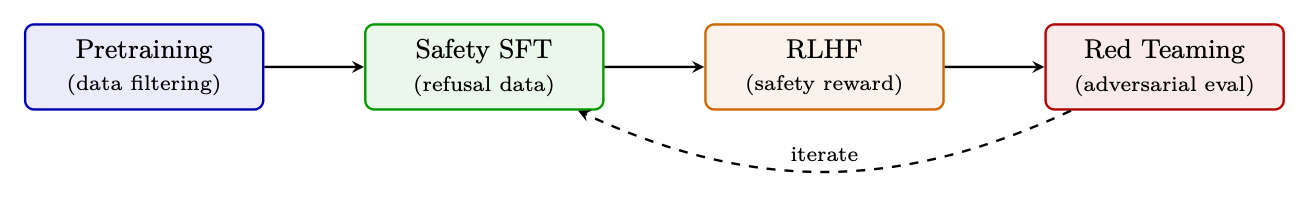
\includegraphics[width=0.85\textwidth]{figures/fig_015_fig15.png}
% \caption{Safety is applied at every stage: data filtering in pretraining, refusal examples in SFT, safety-specific reward models in RLHF, and iterative red-teaming.}
\caption{安全贯穿每个阶段：预训练中的数据过滤、SFT 中的拒答示例、RLHF 中专门的安全奖励模型，以及迭代式红队测试。}
\end{figure}

% \subsection{Key Safety Mechanisms}
\subsection{关键安全机制}
\label{key-safety-mechanisms}

\begin{keybox}[安全技术]
\begin{itemize}
  % \item \textbf{Data filtering}: Remove toxic, biased, and PII-containing text from pretraining corpora
  \item \textbf{数据过滤}：从预训练语料中剔除有毒、有偏见以及含 PII 的文本
  % \item \textbf{Safety SFT}: Train on examples of appropriate refusals (``I can't help with that because\ldots{}'')
  \item \textbf{安全 SFT}：在恰当拒答的示例上训练（``我无法帮你做这件事，因为……''）
  % \item \textbf{Constitutional AI}~\cite{bai2022constitutional}: Self-critique using principles; model revises its own outputs against a constitution of rules
  \item \textbf{宪法 AI（Constitutional AI）}~\cite{bai2022constitutional}：基于原则进行自我批评（Self-Critique）；模型依照一部规则宪法修订自身输出
  % \item \textbf{Safety reward model}: Separate RM trained on safety-annotated pairs; combined with helpfulness RM during RLHF via weighted sum
  \item \textbf{安全奖励模型}：基于安全标注配对训练独立的 RM；在 RLHF 中通过加权和与 helpfulness RM 结合
  % \item \textbf{Guardrails}: Input/output classifiers that block harmful requests/responses at serving time
  \item \textbf{护栏（Guardrails）}：在服务时拦截有害请求/回复的输入/输出分类器
  % \item \textbf{Red teaming}~\cite{perez2022red}: Systematic adversarial evaluation to find failure modes before deployment
  \item \textbf{红队测试（Red teaming）}~\cite{perez2022red}：系统性的对抗评估，在部署前发现失效模式
\end{itemize}
\end{keybox}

% \subsection{The Helpfulness--Safety Tradeoff}
\subsection{有用性与安全性的权衡}
\label{the-helpfulnesssafety-tradeoff}

\begin{intuitionbox}[在有用性与安全性之间平衡]
% Over-optimizing for safety creates an \emph{over-refusal} problem: the model declines benign requests (e.g., refusing to discuss historical violence in an educational context). The goal is a Pareto-optimal policy that is maximally helpful \emph{within} safety constraints:
对安全的过度优化会带来\emph{过度拒答}问题：模型拒绝无害的请求（例如在教育语境中拒绝讨论历史暴力）。目标是一个帕累托最优策略，在安全约束\emph{之内}最大化有用性：
\[
\max_\theta \; \mathbb{E}[R_\text{helpful}] \quad \text{subject to} \quad \mathbb{E}[R_\text{safety}] \geq \tau
\]
% In practice, this is implemented as a weighted reward: $R = \alpha R_\text{helpful} + (1-\alpha) R_\text{safety}$ with careful tuning of $\alpha$ (typically 0.6--0.8). Meta's Llama-3 reports using distinct safety and helpfulness reward models with margin-based weighting~\cite{grattafiori2024llama3}.
在实践中，这通过加权奖励实现：$R = \alpha R_\text{helpful} + (1-\alpha) R_\text{safety}$，并仔细调整 $\alpha$（通常 0.6--0.8）。Meta 的 Llama-3 报告称使用独立的安全与有用性奖励模型，并采用基于 margin 的加权~\cite{grattafiori2024llama3}。
\end{intuitionbox}

% \subsection{Evaluation}
\subsection{评测}
\label{evaluation}

\begin{itemize}
  % \item \textbf{Safety benchmarks}: ToxiGen, RealToxicityPrompts, BBQ (bias), CrowS-Pairs
  \item \textbf{安全基准}：ToxiGen、RealToxicityPrompts、BBQ（偏见）、CrowS-Pairs
  % \item \textbf{Jailbreak robustness}: GCG attacks~\cite{zou2023universal}, multi-turn jailbreaks, encoded prompts
  \item \textbf{越狱鲁棒性}：GCG 攻击~\cite{zou2023universal}、多轮越狱、编码型 Prompt
  % \item \textbf{Over-refusal rate}: Measure false-positive refusals on benign prompts (target $<$5\%)
  \item \textbf{过度拒答率}：度量无害 Prompt 上的假阳性拒答（目标 $<$5\%）
  % \item \textbf{Red team evaluations}: Human adversarial testing with domain experts (biosecurity, cybersecurity)
  \item \textbf{红队评估}：由领域专家（生物安全、网络安全）执行的人类对抗性测试
\end{itemize}

\begin{warningbox}[安全永无完结]
% No combination of techniques provides absolute safety. New attack vectors are discovered continuously (multi-modal jailbreaks, fine-tuning attacks that remove safety training, many-shot prompting). Safety requires ongoing monitoring, rapid response to new threats, and defense-in-depth (multiple independent layers).
任何技术组合都无法提供绝对的安全。新的攻击向量不断被发现（多模态越狱、剥除安全训练的微调攻击、many-shot prompting）。安全需要持续监控、对新威胁的快速响应，以及纵深防御（多层独立防线）。
\end{warningbox}

\chapter{面向 LLM 的系统基础}
\label{systems-foundations-for-llms}

\section{GPU 架构——从硅片到 LLM 训练}
\label{gpu-architecture-from-silicon-to-llm-training}

% Modern large language models are trained and served almost exclusively on GPUs (Graphics Processing Units). Understanding GPU architecture is essential for making informed decisions about parallelism strategies, memory management, kernel optimization, and infrastructure sizing. This section provides a comprehensive introduction to GPU hardware as it relates to LLM workloads.
现代大型语言模型几乎完全依赖 GPU（图形处理器，Graphics Processing Unit）进行训练和服务。理解 GPU 架构对于在并行策略、内存管理、内核优化和基础设施规模等方面做出明智决策至关重要。本节针对 LLM 工作负载，系统地介绍 GPU 硬件相关知识。

\subsection{为什么深度学习要用 GPU？}
\label{why-gpus-for-deep-learning}

% GPUs and CPUs represent fundamentally different hardware philosophies. Understanding this difference explains why LLM training is 100--1000$\times$ faster on GPUs.
GPU 和 CPU 代表了根本不同的硬件设计哲学。理解这种差异能解释为何 LLM 训练在 GPU 上能快 100--1000 倍。

\begin{intuitionbox}[CPU 与 GPU——基本设计哲学]
\begin{itemize}
  % \item \textbf{CPUs} are optimized for \emph{latency} -- they execute a few threads as fast as possible, with large caches, branch predictors, and out-of-order execution. A modern CPU has 8--96 cores.
  \item \textbf{CPU} 针对\emph{延迟}进行优化——它们以尽可能快的速度执行少量线程，配备大型缓存、分支预测器和乱序执行单元。现代 CPU 拥有 8--96 个核心。
  % \item \textbf{GPUs} are optimized for \emph{throughput} -- they execute thousands of threads in parallel, each doing simple work. A modern GPU has thousands of ``cores'' (execution units) grouped into Streaming Multiprocessors (SMs).
  \item \textbf{GPU} 针对\emph{吞吐量}进行优化——它们并行执行数千个线程，每个线程只做简单工作。现代 GPU 拥有数千个“核心”（执行单元），它们被组织成流式多处理器（Streaming Multiprocessor，SM）。
\end{itemize}

% Deep learning workloads are dominated by matrix multiplications ($O(n^3)$ operations on $O(n^2)$ data), which are embarrassingly parallel. A single transformer forward pass for a 70B model requires $\sim$140 TFLOP of compute per token -- perfect for GPU throughput.
深度学习工作负载以矩阵乘法（在 $O(n^2)$ 数据上执行 $O(n^3)$ 操作）为主，这是天然并行的。70B 模型的单次 transformer 前向传播每个 token 需要约 140 TFLOP 计算量——非常适合 GPU 的吞吐能力。
\end{intuitionbox}

\subsection{NVIDIA GPU 微架构代际演进}
\label{nvidia-gpu-microarchitecture-generations}

% NVIDIA has released a series of GPU architectures, each bringing key innovations for deep learning:
NVIDIA 已经发布了一系列 GPU 架构，每一代都为深度学习带来关键创新：

\begin{table}[ht!]
\centering\small
\caption{面向深度学习的 NVIDIA GPU 微架构时间线。}
\noindent\begin{tabularx}{\linewidth}{@{}l Z{0.3} Z{0.3} Z{2.4}@{}}
\toprule
\textbf{架构} & \textbf{年份} & \textbf{旗舰} & \textbf{深度学习关键创新} \\
\midrule
Pascal & 2016 & P100 & 首款 HBM GPU；FP16 支持；NVLink 1 \\
Volta & 2017 & V100 & \textbf{Tensor Cores}（第一代）；混合精度训练 \\
Turing & 2018 & T4 & INT8 推理；RT cores（非 ML 用途） \\
Ampere & 2020 & A100 & BF16 Tensor Cores；TF32；第 3 代 NVLink；MIG \\
Hopper & 2022 & H100 & FP8 Tensor Cores；TMA；Transformer Engine；NVLink 4 \\
Blackwell & 2024 & B200 & 第 2 代 Transformer Engine；NVLink 5（1.8 TB/s）；FP4 \\
\bottomrule
\end{tabularx}
\end{table}

\subsection{LLM 训练与推理常用 GPU}
\label{common-gpus-for-llm-training-and-inference}

\begin{table}[ht!]
\centering
\caption{与 LLM 工作负载相关的 GPU 规格。所有带宽数字均为双向。}
\footnotesize
\noindent\begin{tabularx}{\linewidth}{@{}l l l l l l Z{1}@{}}
\toprule
\textbf{GPU} & \textbf{架构} & \textbf{HBM} & \textbf{BF16 TF} & \textbf{HBM 带宽} & \textbf{NVLink} & \textbf{LLM 角色} \\
\midrule
V100-32GB & Volta & 32 GB & 125 TF* & 900 GB/s & 300 GB/s & 旧型号；小模型微调 \\
A100-40GB & Ampere & 40 GB & 312 TF & 1.5 TB/s & 600 GB/s & 经济型训练/推理 \\
A100-80GB & Ampere & 80 GB & 312 TF & 2.0 TB/s & 600 GB/s & 标准 RLHF（70B 模型用 8--64 卡） \\
H100 SXM & Hopper & 80 GB & 990 TF & 3.35 TB/s & 900 GB/s & 训练快 3$\times$ \\
H200 SXM & Hopper & 141 GB & 990 TF & 4.8 TB/s & 900 GB/s & 用更少 GPU 装下 70B 策略+参考模型 \\
B200 SXM & Blackwell & 192 GB & 2250 TF & 8.0 TB/s & 1800 GB/s & 新一代；比 H100 快 2$\times$ \\
\midrule
\multicolumn{7}{@{}l}{\emph{AMD 和 Google 替代方案：}} \\
MI300X & CDNA3 & 192 GB & 1300 TF & 5.3 TB/s & N/A & 显存最大；ROCm \\
TPU v5e & Google & 16 GB & 197 TF & 1.6 TB/s & ICI 1.6 TB/s & 仅云端；JAX/XLA \\
\bottomrule
\end{tabularx}
\end{table}

\begin{warningbox}[如何选择 GPU？]
\begin{itemize}
  % \item \textbf{Training 70B+ models}: H100/B200 nodes with NVLink (need fast interconnect for tensor parallelism). Minimum 8$\times$H100 per instance.
  \item \textbf{训练 70B+ 模型}：带 NVLink 的 H100/B200 节点（张量并行需要快速互联）。每个实例至少 8$\times$H100。
  % \item \textbf{Inference (latency-sensitive)}: H100/H200 for high BW; MI300X for memory-bound (huge KV caches).
  \item \textbf{推理（延迟敏感）}：H100/H200 适合高带宽场景；MI300X 适合内存密集（Memory-Bound）场景（巨大的键值缓存（KV Cache））。
  % \item \textbf{Fine-tuning 7B--13B}: A100-80GB is cost-effective. Single GPU with LoRA.
  \item \textbf{微调 7B--13B 模型}：A100-80GB 性价比高。用 LoRA 单卡即可。
  % \item \textbf{Budget}: A100-40GB or even A10 (24GB) for LoRA on 7B models.
  \item \textbf{预算紧张}：A100-40GB，甚至用 A10（24GB）在 7B 模型上跑 LoRA。
\end{itemize}
\end{warningbox}

\subsection{GPU 内部架构——流式多处理器（SM）}
\label{gpu-internal-architecture-the-streaming-multiprocessor-sm}

% A GPU is organized as an array of \textbf{Streaming Multiprocessors (SMs)}, each of which is an independent processor with its own register file, shared memory, and execution units. Understanding SMs is key to understanding GPU performance.
GPU 由一组\textbf{流式多处理器（Streaming Multiprocessor，SM）}阵列组成，每个 SM 都是独立的处理器，拥有自己的寄存器文件、共享内存和执行单元。理解 SM 是理解 GPU 性能的关键。

\begin{figure}[ht!]
\centering
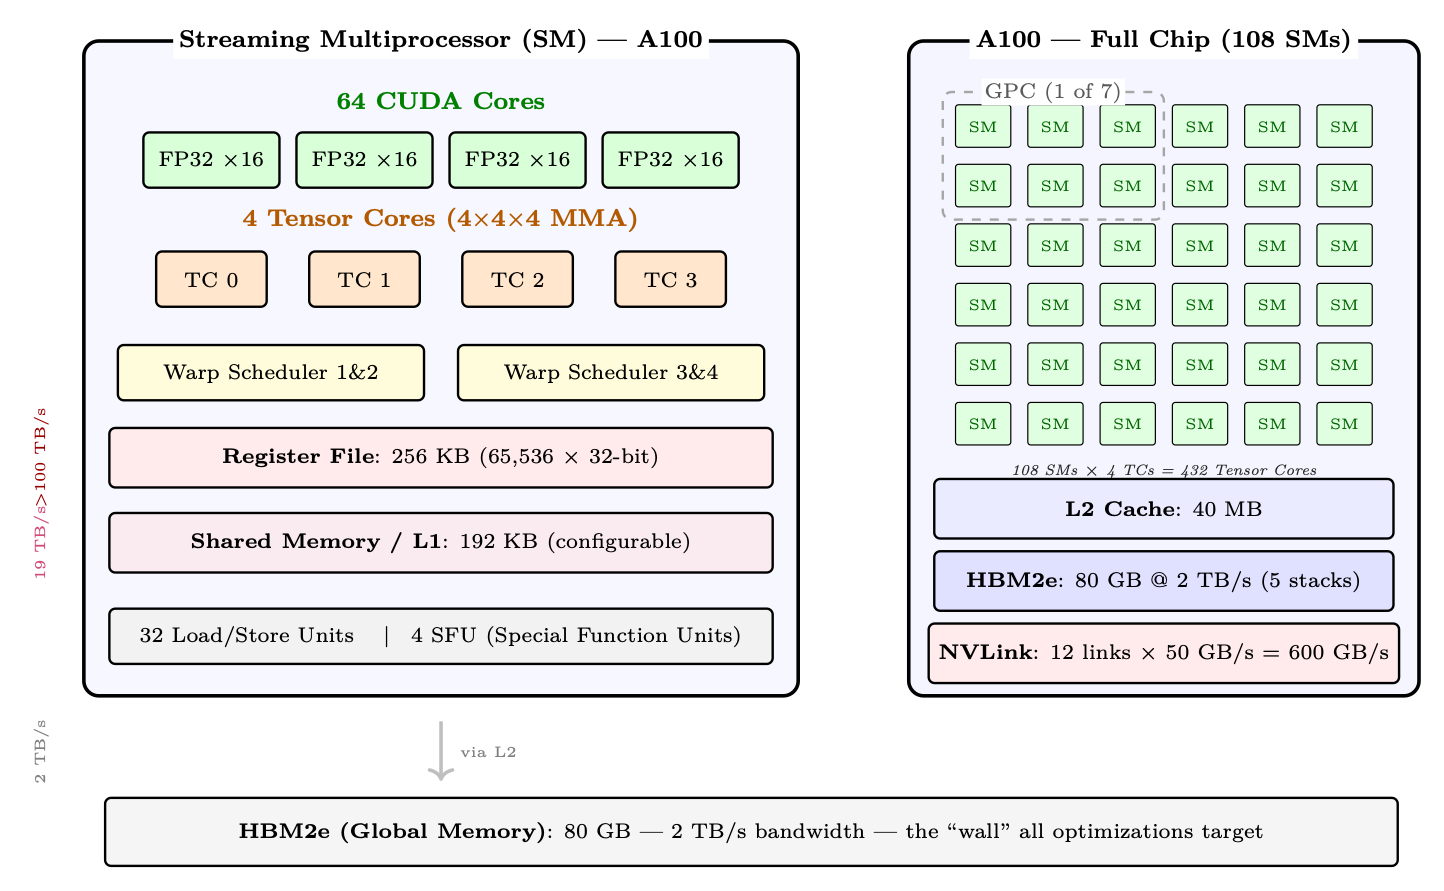
\includegraphics[width=0.85\textwidth]{figures/fig_016_fig16.png}
\caption{左：A100 单个流式多处理器（SM）的内部结构——64 个 FP32 CUDA cores、4 个 Tensor Cores、4 个 warp 调度器、256 KB 寄存器文件以及 192 KB 共享内存/L1 缓存。右：完整 A100 芯片包含 108 个 SM，共享 40 MB L2 缓存和 80 GB HBM2e。左侧边栏的带宽标注显示了从寄存器到 HBM 的急剧下降。}
\end{figure}

\begin{keybox}[SM 的关键组件]
\begin{itemize}
  % \item \textbf{CUDA Cores:} Scalar ALUs for FP32/INT32 operations. 64 per SM on A100. Used for element-wise ops, reductions, and non-matrix operations.
  \item \textbf{CUDA Cores：}用于 FP32/INT32 运算的标量 ALU。A100 上每个 SM 有 64 个。用于逐元素运算、归约和非矩阵运算。
  % \item \textbf{Tensor Cores:} Specialized matrix-multiply-accumulate (MMA) units. Each performs a $4{\times}4{\times}4$ fused multiply-add per cycle. 4 per SM on A100, delivering $16\times$ throughput over CUDA cores for supported precisions.
  \item \textbf{Tensor Cores：}专用的矩阵乘加（matrix-multiply-accumulate，MMA）单元。每个单元每周期执行一次 $4{\times}4{\times}4$ 融合乘加运算。A100 每个 SM 有 4 个，在支持的精度下提供相对 CUDA cores $16\times$ 的吞吐量。
  % \item \textbf{Register File:} Fastest storage (1 cycle latency). Shared among all active threads. Spilling to L1 causes significant slowdown.
  \item \textbf{寄存器文件：}最快的存储（延迟 1 周期）。所有活动线程共享。溢出到 L1 会显著降速。
  % \item \textbf{Shared Memory / L1:} On-chip SRAM explicitly managed by the programmer. The key to FlashAttention's performance (tiles fit entirely in shared memory).
  \item \textbf{共享内存 / L1：}由程序员显式管理的片上 SRAM。这是 FlashAttention 性能的关键（数据块完全装入共享内存）。
  % \item \textbf{Warp Schedulers:} Each SM has 4 warp schedulers (A100). A \emph{warp} = 32 threads executing in lockstep (SIMT model). Schedulers hide memory latency by switching between warps.
  \item \textbf{Warp 调度器：}每个 SM 有 4 个 warp 调度器（A100）。一个 \emph{warp} = 32 个步调一致执行的线程（SIMT 模型）。调度器通过在 warp 之间切换来隐藏内存延迟。
\end{itemize}
\end{keybox}

\begin{intuitionbox}[SIMT 执行模型]
% GPUs use Single Instruction, Multiple Threads (SIMT) execution. Within a warp (32 threads), all threads execute the same instruction but on different data. When threads diverge (e.g., \texttt{if/else}), both paths are serialized -- called \emph{warp divergence}. This is why GPU kernels must minimize branching.
GPU 采用单指令多线程（Single Instruction, Multiple Threads，SIMT）执行模型。在一个 warp（32 个线程）内，所有线程执行相同指令但作用于不同数据。当线程出现分支（例如 \texttt{if/else}）时，两条路径都会被串行执行——称为 \emph{warp 分支（warp divergence）}。这就是为什么 GPU 内核必须最小化分支的原因。

% For LLM workloads, the main operations (GEMM, attention, softmax) have uniform control flow across threads, making them ideal for SIMT execution.
对于 LLM 工作负载，主要运算（GEMM、attention、softmax）在线程间具有统一的控制流，非常适合 SIMT 执行。
\end{intuitionbox}

\subsection{各代际 GPU 芯片的扩展}
\label{gpu-chip-scaling-across-generations}

% The evolution of NVIDIA's GPU architectures shows consistent scaling of compute density, on-chip memory, and specialized units for deep learning:
NVIDIA GPU 架构的演进显示出在计算密度、片上内存和深度学习专用单元方面持续扩展：

\begin{table}[ht!]
\centering
\caption{各代 NVIDIA 架构在 SM 层面的扩展。}
\small
\noindent\begin{tabularx}{\linewidth}{@{}l l l l l Z{1}@{}}
\toprule
\textbf{架构} & \textbf{SM 数} & \textbf{TCs/SM} & \textbf{SRAM/SM} & \textbf{L2} & \textbf{关键变化} \\
\midrule
Volta (V100) & 80 & 8 & 128 KB & 6 MB & 引入 Tensor Cores \\
Ampere (A100) & 108 & 4 & 192 KB & 40 MB & BF16/TF32；更大的 L2 \\
Hopper (H100) & 132 & 4 & 256 KB & 50 MB & TMA；FP8；Thread Block Clusters \\
Blackwell (B200) & 148 & 4 & 256 KB & 128 MB & 2$\times$ 裸片；FP4；TMEM；NVLink 5 \\
\bottomrule
\end{tabularx}
\end{table}

\subsection{GPU 内存层级与带宽}
\label{gpu-memory-hierarchy-and-bandwidth}

% Modern GPU training and inference performance is almost entirely determined by \emph{how well you manage data movement} across the memory hierarchy. Understanding the hierarchy is not optional -- it is the foundation for every optimization technique discussed in later sections.
现代 GPU 训练和推理性能几乎完全取决于\emph{你如何管理数据在内存层级之间的搬运}。理解内存层级不是可选项——它是后续章节讨论每一种优化技术的基础。

\begin{keybox}[GPU 内存层级——A100 80GB 参考数字]
\small
\begin{center}
\begin{tabularx}{0.82\linewidth}{@{}l l l l Z{1}@{}}
\toprule
\textbf{层级} & \textbf{容量} & \textbf{带宽} & \textbf{延迟} & \textbf{位置} \\
\midrule
寄存器 & $\sim$256 KB/SM & $>$100 TB/s & 1 周期 & 片上，每线程 \\
SRAM (shared) & 164 KB/SM & $\sim$19 TB/s & $\sim$20 周期 & 片上，每 SM \\
L2 缓存 & 共 40 MB & $\sim$5 TB/s & $\sim$200 周期 & 片上，共享 \\
HBM2e (VRAM) & 80 GB & 2 TB/s & $\sim$200 ns & 封装上（5 个堆栈） \\
CPU DRAM & 512 GB+ & $\sim$25 GB/s & $\sim$10 $\mu$s & 主机（PCIe 4） \\
NVMe SSD & TB 级 & 7 GB/s & $\sim$100 $\mu$s & 主机存储 \\
\bottomrule
\end{tabularx}
\end{center}
\end{keybox}

\begin{intuitionbox}[为何各层级差距如此巨大]
% Each level of the hierarchy is roughly \textbf{10$\times$ slower and 100--1000$\times$ larger} than the one above it. The A100 has 312 TFLOP/s of BF16 tensor-core throughput but only 2 TB/s of HBM bandwidth. That means for every byte loaded from HBM you can do $312 \times 10^{12} / (2 \times 10^{12}) \approx 156$ floating-point operations before the next byte arrives. If your kernel does fewer than 156 FLOPs per byte, it is \emph{memory-bound} -- the compute units are idle waiting for data.
内存层级中每一级大约比上一级\textbf{慢 10$\times$，大 100--1000$\times$}。A100 有 312 TFLOP/s 的 BF16 tensor-core 吞吐，但 HBM 带宽只有 2 TB/s。这意味着从 HBM 每加载一字节，你可以在下一字节到达之前完成 $312 \times 10^{12} / (2 \times 10^{12}) \approx 156$ 次浮点运算。如果你的内核每字节运算少于 156 FLOPs，它就是\emph{内存密集（Memory-Bound）}的——计算单元在空等数据。
\end{intuitionbox}

\paragraph{寄存器。}
\label{registers.}

% Each CUDA thread has access to a private register file. Registers are the fastest storage on the chip -- reads and writes happen in a single clock cycle with no arbitration. The A100 has 65,536 32-bit registers per SM. Spilling registers to local memory (L1/L2) is a major performance hazard.
每个 CUDA 线程都有自己的私有寄存器文件。寄存器是芯片上最快的存储——读写在一个时钟周期内完成且无需仲裁。A100 每个 SM 有 65,536 个 32 位寄存器。寄存器溢出到本地内存（L1/L2）是主要的性能隐患。

\paragraph{SRAM——共享内存 / L1。}
\label{sram-shared-memory-l1.}

% Each SM has a combined L1/shared memory pool of 192 KB on A100 (256 KB on H100), with up to 164 KB configurable as shared memory on A100. Shared memory is explicitly managed by the programmer (or by the compiler in newer CUDA versions). FlashAttention, for example, is entirely built around the insight that the attention tile computation fits in SRAM.
A100 上每个 SM 拥有 192 KB 的 L1/共享内存池（H100 为 256 KB），其中最多 164 KB 可配置为共享内存。共享内存由程序员（或较新版本 CUDA 中由编译器）显式管理。例如，FlashAttention 的整个设计都基于一个洞察：注意力分块计算可以装入 SRAM。

\paragraph{L2 缓存。}
\label{l2-cache.}

% The 40 MB L2 on A100 is shared across all 108 SMs. It acts as a staging area between SRAM and HBM. For workloads with good spatial locality (e.g., weight matrices accessed repeatedly across a batch), L2 hit rates can dramatically reduce effective HBM traffic.
A100 上的 40 MB L2 由所有 108 个 SM 共享。它充当 SRAM 与 HBM 之间的中转区。对于具有良好空间局部性的工作负载（例如在一个 batch 内被反复访问的权重矩阵），L2 命中率可以大幅降低实际 HBM 流量。

\paragraph{HBM——高带宽显存。}
\label{hbm-high-bandwidth-memory.}

% HBM is stacked DRAM mounted directly on the GPU package, connected via a wide interposer. The A100 SXM has 80 GB of HBM2e at 2 TB/s. The H100 SXM5 has 80 GB of HBM3 at 3.35 TB/s. This is the primary working memory for model weights, KV caches, activations, and optimizer states.
高带宽显存（High Bandwidth Memory，HBM）是直接安装在 GPU 封装上的堆叠 DRAM，通过宽带中介层连接。A100 SXM 拥有 80 GB HBM2e，带宽 2 TB/s；H100 SXM5 拥有 80 GB HBM3，带宽 3.35 TB/s。它是模型权重、KV cache、激活和优化器状态的主要工作内存。

\paragraph{通过 PCIe 访问 CPU DRAM。}
\label{cpu-dram-via-pcie.}

% Data transfer between GPU HBM and CPU DRAM traverses the PCIe bus. PCIe Gen4 $\times$16 provides $\sim$32 GB/s per direction (64 GB/s bidirectional); Gen5 doubles this. This is a $\sim$60$\times$ bandwidth reduction compared to HBM (per-direction). CPU offloading (ZeRO-Infinity, DeepSpeed) exploits this link but must be used carefully to avoid becoming the bottleneck.
GPU HBM 与 CPU DRAM 之间的数据传输需经过 PCIe 总线。PCIe Gen4 $\times$16 每方向提供约 32 GB/s（双向 64 GB/s）；Gen5 翻倍。这相对于 HBM（每方向）是约 60$\times$ 的带宽下降。CPU 卸载（ZeRO-Infinity、DeepSpeed）利用这条链路，但必须谨慎使用以免成为瓶颈。

\paragraph{NVMe。}
\label{nvme.}

% NVMe SSDs (e.g., Samsung 990 Pro) reach $\sim$7 GB/s sequential read. ZeRO-Infinity can offload optimizer states to NVMe, but this is only viable when the compute-to-IO ratio is very high (large batch sizes, slow training steps).
NVMe SSD（例如 Samsung 990 Pro）顺序读取可达约 7 GB/s。ZeRO-Infinity 可以将优化器状态卸载到 NVMe，但只有在计算与 I/O 比率非常高（大 batch 尺寸、训练步骤较慢）时才可行。

\subsection{算术强度与 Roofline 模型}
\label{arithmetic-intensity-and-the-roofline-model}

\begin{keybox}[算术强度（Arithmetic Intensity）]
\[
I = \frac{\text{FLOPs}}{\text{从 HBM 访问的字节数}}
  \quad \text{(FLOPs / Byte)}
\]
% A kernel is \textbf{memory-bound} when $I < I_{\text{ridge}}$ and \textbf{compute-bound} when $I > I_{\text{ridge}}$, where
当 $I < I_{\text{ridge}}$ 时内核是\textbf{内存密集（Memory-Bound）}的，当 $I > I_{\text{ridge}}$ 时则是\textbf{计算密集（Compute-Bound）}的，其中
\[
I_{\text{ridge}} = \frac{\text{峰值 FLOP/s}}{\text{峰值带宽}}
  = \frac{312 \times 10^{12}}{2 \times 10^{12}} = 156 \text{ FLOP/Byte (A100 BF16)}
\]
\end{keybox}

\begin{figure}[ht!]
\centering
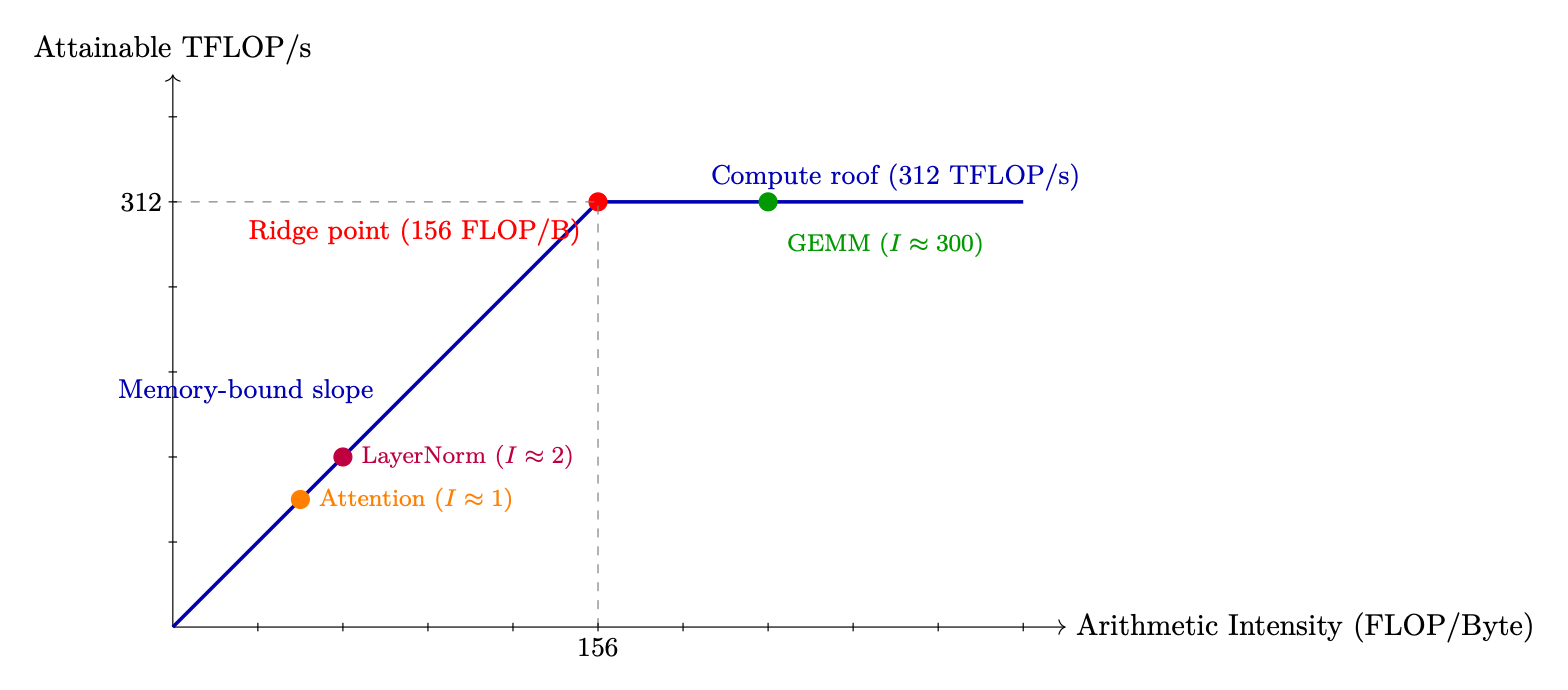
\includegraphics[width=0.85\textwidth]{figures/fig_017_fig17.png}
\caption{A100 BF16 的 Roofline 模型（Roofline Model）。Attention 深陷于内存密集区间；大型 GEMM（FFN 层）则是计算密集的。}
\end{figure}

\begin{examplebox}[Attention 的算术强度]
% For a single attention head with sequence length $n=4096$, head dim $d=128$:
对于序列长度 $n=4096$、头维度 $d=128$ 的单个注意力头：

% \textbf{FLOPs}: $QK^T$ costs $2n^2d$, softmax is $O(n^2)$, $\text{Attn} \times V$ costs $2n^2d$. Total: $\approx 4n^2 d = 4 \times 4096^2 \times 128 \approx 8.6$ GFLOP.
\textbf{FLOPs}：$QK^T$ 耗费 $2n^2d$，softmax 为 $O(n^2)$，$\text{Attn} \times V$ 耗费 $2n^2d$。总计：$\approx 4n^2 d = 4 \times 4096^2 \times 128 \approx 8.6$ GFLOP。

% \textbf{Memory traffic} (standard, non-Flash implementation):
\textbf{内存流量}（标准实现，非 Flash 版）：

\begin{itemize}
  % \item Read $Q, K$: $2 \times n \times d \times 2 = 2$ MB
  \item 读取 $Q, K$：$2 \times n \times d \times 2 = 2$ MB
  % \item Write attention scores $S = QK^T$: $n^2 \times 2 = 33.5$ MB
  \item 写入注意力分数 $S = QK^T$：$n^2 \times 2 = 33.5$ MB
  % \item Read $S$ for softmax: $n^2 \times 2 = 33.5$ MB
  \item 为 softmax 读取 $S$：$n^2 \times 2 = 33.5$ MB
  % \item Write softmax output $P$: $n^2 \times 2 = 33.5$ MB
  \item 写入 softmax 输出 $P$：$n^2 \times 2 = 33.5$ MB
  % \item Read $P$ and $V$ for final matmul: $n^2 \times 2 + n \times d \times 2 = 34.5$ MB
  \item 为最终矩阵乘读取 $P$ 和 $V$：$n^2 \times 2 + n \times d \times 2 = 34.5$ MB
  % \item Write output $O$: $n \times d \times 2 = 1$ MB
  \item 写入输出 $O$：$n \times d \times 2 = 1$ MB
\end{itemize}

% \textbf{Total memory}: $\approx 138$ MB (dominated by 4 passes over the $n^2$ attention matrix).
\textbf{总内存}：$\approx 138$ MB（由对 $n^2$ 注意力矩阵的 4 次遍历主导）。

% \textbf{Arithmetic intensity}:
\textbf{算术强度}：
\[
I = \frac{8.6 \times 10^9}{138 \times 10^6} \approx 62 \text{ FLOP/Byte}
\]

% This is $62/156 = 40\%$ of the A100 ridge point --- \textbf{firmly memory-bound}. The GPU is 60\% idle waiting for memory.
这是 A100 脊点的 $62/156 = 40\%$——\textbf{明确属于内存密集}。GPU 有 60\% 的时间在等内存空转。

% \textbf{FlashAttention fix}: By never materializing the $n \times n$ matrix (tiling $Q, K, V$ in SRAM), FlashAttention reduces HBM traffic to just reading $Q, K, V$ and writing $O$: $4 \times n \times d \times 2 = 4$ MB. Each byte loaded is reused in $O(n)$ computations (every query attends to every key), so:
\textbf{FlashAttention 解决方案}：通过永远不物化 $n \times n$ 矩阵（在 SRAM 中对 $Q, K, V$ 分块），FlashAttention 把 HBM 流量降至仅读取 $Q, K, V$ 并写入 $O$：$4 \times n \times d \times 2 = 4$ MB。每个加载的字节被复用于 $O(n)$ 次计算（每个 query 都要 attend 所有 key），因此：
\[
I = \frac{4n^2 d}{4 \cdot n \cdot d \cdot 2} = \frac{n}{2} = \frac{4096}{2} = 2048 \text{ FLOP/Byte}
\]

% This is $13\times$ above the ridge point (156) --- \textbf{deeply compute-bound}. The GPU hits its peak 312 TFLOPS, needing only $312\text{T}/2048 \approx 152$ GB/s of bandwidth (7.6\% of HBM capacity). Memory is no longer the bottleneck.
这比脊点（156）高出 $13\times$——\textbf{深度计算密集}。GPU 跑满峰值 312 TFLOPS，只需要 $312\text{T}/2048 \approx 152$ GB/s 带宽（HBM 容量的 7.6\%）。内存不再是瓶颈。
\end{examplebox}

\subsection{Attention 是内存密集的；FFN 是计算密集的}
\label{attention-is-memory-bound-ffn-is-compute-bound}

\begin{intuitionbox}[Transformer 中的两种区间]
% A transformer block has two main components with very different arithmetic intensities:
一个 transformer 块有两个主要组件，它们的算术强度截然不同：

\begin{itemize}
  % \item \textbf{Attention:} Operates on $n \times d$ tensors. The $QK^T$ product is $O(n^2 d)$ FLOPs but requires $O(n^2)$ memory for the attention scores. At long sequences, memory traffic dominates -- attention is \emph{memory-bound}.
  \item \textbf{Attention：}作用于 $n \times d$ 张量。$QK^T$ 乘积是 $O(n^2 d)$ FLOPs，但注意力分数需要 $O(n^2)$ 内存。在长序列下，内存流量占主导地位——attention 是\emph{内存密集（Memory-Bound）}的。
  % \item \textbf{FFN (MLP):} Two large linear layers with weight matrices of shape $[d_{\text{model}}, 4d_{\text{model}}]$. These are large GEMMs with high arithmetic intensity -- FFN is \emph{compute-bound}.
  \item \textbf{FFN（MLP）：}两个大型线性层，权重矩阵形状为 $[d_{\text{model}}, 4d_{\text{model}}]$。这些是高算术强度的大型 GEMM——FFN 是\emph{计算密集（Compute-Bound）}的。
\end{itemize}

% This is why FlashAttention (memory optimization) helps attention but not FFN, while quantization (reducing weight size) helps FFN more than attention.
这就是为什么 FlashAttention（内存优化）对 attention 有效但对 FFN 无效，而量化（缩小权重体积）对 FFN 的帮助比对 attention 更大。
\end{intuitionbox}

\subsection{Tensor Cores}
\label{tensor-cores}

\begin{keybox}[什么是 Tensor Cores？]
% Tensor Cores are specialized matrix-multiply-accumulate (MMA) units introduced in Volta (2017). Each Tensor Core performs a $4\times4\times4$ matrix multiply in a single clock cycle:
张量核心（Tensor Core）是 Volta 架构（2017）引入的专用矩阵乘加（MMA）单元。每个 Tensor Core 在单个时钟周期内执行一次 $4\times4\times4$ 矩阵乘法：
\[
D = A \times B + C \quad (4\times4 \text{ matrices})
\]
% The A100 has \textbf{432 Tensor Cores} across 108 SMs (4 per SM, one per sub-partition). At BF16 precision, they deliver 312 TFLOP/s -- roughly $16\times$ the throughput of FP32 CUDA cores.
A100 在 108 个 SM 中共有 \textbf{432 个 Tensor Cores}（每个 SM 4 个，每个子分区 1 个）。在 BF16 精度下提供 312 TFLOP/s 吞吐——约是 FP32 CUDA cores 吞吐的 $16\times$。
\end{keybox}

\begin{itemize}
  % \item \textbf{Supported precisions:} FP64, TF32, BF16, FP16, INT8, FP8 (H100+).
  \item \textbf{支持的精度：}FP64、TF32、BF16、FP16、INT8、FP8（H100+）。
  % \item \textbf{Accumulation:} Always in FP32 internally, even for BF16 inputs. This prevents catastrophic cancellation during the dot product.
  \item \textbf{累加：}内部始终使用 FP32，即使输入为 BF16。这能防止点积过程中的灾难性抵消。
  % \item \textbf{Requirement:} Tensor Cores are most efficient when matrix dimensions are multiples of 8 (BF16) or 16 (FP8). Padding to these multiples is often worthwhile.
  \item \textbf{要求：}当矩阵维度是 8（BF16）或 16（FP8）的倍数时，Tensor Cores 效率最高。为此进行填充通常是值得的。
  % \item \textbf{WGMMA (H100):} Hopper introduces warpgroup-level MMA instructions that operate on larger tiles (64$\times$256$\times$16) and can be pipelined with TMA (Tensor Memory Accelerator) data movement.
  \item \textbf{WGMMA（H100）：}Hopper 引入了 warpgroup 级别的 MMA 指令，作用于更大的分块（64$\times$256$\times$16），并可与 TMA（Tensor Memory Accelerator）数据搬运形成流水线。
\end{itemize}

\begin{warningbox}[Tensor Core 陷阱]
% Tensor Cores only help if your kernel is \emph{compute-bound}. If you are running a small batch (batch size 1, inference), the GEMM tiles are tiny, Tensor Core utilization is low, and you are back in the memory-bound regime. This is why inference engines batch requests aggressively.
只有当你的内核是\emph{计算密集（Compute-Bound）}时，Tensor Cores 才有用。如果你跑的是小 batch（batch size 1 的推理），GEMM 分块很小，Tensor Core 利用率很低，你又回到内存密集区间。这就是为什么推理引擎要激进地对请求进行 batch。
\end{warningbox}

\subsection{通信架构——NVLink、InfiniBand 与 PCIe}
\label{communication-architecture-nvlink-infiniband-and-pcie}

% Distributed LLM training and inference require moving enormous amounts of data between GPUs, nodes, and storage. The communication fabric is often the bottleneck for large-scale training.
分布式 LLM 训练和推理需要在 GPU、节点和存储之间搬运海量数据。通信结构往往是大规模训练的瓶颈。

\paragraph{PCIe——主机与设备的链路。}
\label{pcie-the-host-device-link.}

\begin{keybox}[PCIe 各代]
\begin{center}
\begin{tabular}{@{}l l l l@{}}
\toprule
\textbf{代际} & \textbf{x16 带宽（每方向）} & \textbf{双向} & \textbf{备注} \\
\midrule
PCIe Gen3 & 16 GB/s & 32 GB/s & 常见于较旧服务器 \\
PCIe Gen4 & 32 GB/s & 64 GB/s & A100 PCIe、当前主流服务器 \\
PCIe Gen5 & 64 GB/s & 128 GB/s & H100 PCIe，正在普及 \\
\bottomrule
\end{tabular}
\end{center}
\end{keybox}

% PCIe is used for:
PCIe 用于：

\begin{itemize}
  % \item CPU $\leftrightarrow$ GPU data transfers (model loading, CPU offloading)
  \item CPU $\leftrightarrow$ GPU 数据传输（模型加载、CPU 卸载）
  % \item Cross-node GPU communication when NVLink is unavailable (rare, very slow)
  \item 当 NVLink 不可用时的跨节点 GPU 通信（罕见，且非常慢）
  % \item NVMe storage access (via CPU)
  \item NVMe 存储访问（经由 CPU）
\end{itemize}

\begin{warningbox}[PCIe 不应用于 GPU 间通信]
% Never route GPU-GPU communication through PCIe if NVLink is available. PCIe bandwidth (32 GB/s) is 28$\times$ lower than NVLink 4 (900 GB/s). In a multi-GPU server without NVLink (e.g., consumer GPUs), inter-GPU bandwidth is limited to PCIe, making tensor parallelism extremely slow.
如果有 NVLink 可用，绝不要让 GPU-GPU 通信走 PCIe。PCIe 带宽（32 GB/s）比 NVLink 4（900 GB/s）低 28$\times$。在没有 NVLink 的多 GPU 服务器中（例如消费级 GPU），GPU 间带宽被限制在 PCIe 水平，使得张量并行极其缓慢。
\end{warningbox}

\newpage
\paragraph{NVLink——节点内高速互联。}
\label{nvlink-intra-node-high-speed-interconnect.}
\nopagebreak
\begin{keybox}[NVLink 各代]
\begin{center}
\begin{tabular}{@{}l l l l@{}}
\toprule
\textbf{代际} & \textbf{链路数} & \textbf{总带宽} & \textbf{GPU} \\
\midrule
NVLink 2 & 6 & 300 GB/s & V100 \\
NVLink 3 & 12 & 600 GB/s & A100 \\
NVLink 4 & 18 & 900 GB/s & H100 \\
NVLink 5 & 18 & 1800 GB/s & B200 (Blackwell) \\
\bottomrule
\end{tabular}
\end{center}
\end{keybox}

% NVLink is a point-to-point interconnect between GPUs on the same node. Each link is bidirectional. The H100 SXM5 has 18 NVLink 4 links, each providing 50 GB/s bidirectional, for a total of 900 GB/s.
NVLink 是同一节点内 GPU 之间的点对点互联。每条链路都是双向的。H100 SXM5 拥有 18 条 NVLink 4 链路，每条提供 50 GB/s 双向带宽，总计 900 GB/s。

\paragraph{NVSwitch。}
\label{nvswitch.}

% In DGX H100 systems, all 8 GPUs are connected via NVSwitch -- a dedicated switching chip that provides \emph{full bisection bandwidth}. This means any GPU can communicate with any other GPU at full NVLink speed simultaneously, not just neighbors in a ring.
在 DGX H100 系统中，所有 8 块 GPU 都通过 NVSwitch 互联——这是一种提供\emph{全二分带宽（full bisection bandwidth）}的专用交换芯片。这意味着任意 GPU 都能以完整 NVLink 速度同时与任何其他 GPU 通信，而不仅仅是环上邻居。

\begin{intuitionbox}[环形拓扑 vs. 全二分]
% In a ring topology (8 GPUs), an AllReduce requires data to travel around the ring. Each link must carry $\frac{2(N-1)}{N}$ of the total data, so the algorithm bandwidth is $B_{\text{link}} \times \frac{N}{2(N-1)}$ (about $0.57 \times B_{\text{link}}$ for $N=8$). With NVSwitch full bisection, AllReduce can use all links simultaneously with tree-based algorithms, achieving near-peak bandwidth. In practice on DGX H100: ring achieves $\sim$700 GB/s bus bandwidth, NVSwitch achieves $\sim$900 GB/s.
在环形拓扑（8 GPU）中，AllReduce 需要数据绕环传输。每条链路必须承载总数据的 $\frac{2(N-1)}{N}$，因此算法带宽为 $B_{\text{link}} \times \frac{N}{2(N-1)}$（$N=8$ 时约为 $0.57 \times B_{\text{link}}$）。借助 NVSwitch 的全二分带宽，AllReduce 可以使用基于树的算法同时使用所有链路，达到接近峰值的带宽。在 DGX H100 实际测试中：ring 达到约 700 GB/s 总线带宽，NVSwitch 达到约 900 GB/s。
\end{intuitionbox}

\paragraph{InfiniBand——节点间通信。}
\label{infiniband-inter-node-communication.}

% For communication between nodes (servers), InfiniBand provides high-bandwidth, low-latency networking with direct GPU memory access.
对于节点（服务器）之间的通信，InfiniBand 提供高带宽、低延迟的网络，并支持直接 GPU 内存访问。

\begin{keybox}[InfiniBand NDR]
\begin{itemize}
  % \item \textbf{NDR 400Gb/s} = 50 GB/s per port (unidirectional)
  \item \textbf{NDR 400Gb/s} = 每端口 50 GB/s（单向）
  % \item \textbf{HDR 200Gb/s} = 25 GB/s per port (previous generation)
  \item \textbf{HDR 200Gb/s} = 每端口 25 GB/s（上一代）
  % \item \textbf{RDMA:} Remote Direct Memory Access -- GPU can read/write remote GPU memory without involving the remote CPU
  \item \textbf{RDMA：}远程直接内存访问（Remote Direct Memory Access）——GPU 可读写远端 GPU 内存而无需远端 CPU 参与
  % \item \textbf{GPUDirect RDMA:} Data goes directly HBM $\to$ NIC $\to$ network $\to$ NIC $\to$ HBM, bypassing CPU and system DRAM entirely
  \item \textbf{GPUDirect RDMA：}数据直接经由 HBM $\to$ NIC $\to$ 网络 $\to$ NIC $\to$ HBM，完全绕过 CPU 和系统 DRAM
  % \item \textbf{Latency:} $\sim$1--2 $\mu$s for small messages (vs.~$\sim$100 $\mu$s for TCP/IP)
  \item \textbf{延迟：}小消息约 1--2 $\mu$s（对比 TCP/IP 的约 100 $\mu$s）
\end{itemize}
\end{keybox}

\paragraph{胖树拓扑（Fat-Tree Topology）。}
\label{fat-tree-topology.}

% Large GPU clusters use fat-tree network topologies. A 3-level fat-tree with $k$-port switches supports $k^3/4$ nodes with full bisection bandwidth. For 400Gb/s NDR switches with $k=64$ ports: $64^3/4 = 65{,}536$ nodes.
大型 GPU 集群使用胖树（Fat-Tree Topology）网络拓扑。使用 $k$ 端口交换机的 3 层胖树可支持 $k^3/4$ 个节点并保持全二分带宽。对于 $k=64$ 端口的 400Gb/s NDR 交换机：$64^3/4 = 65{,}536$ 个节点。

\paragraph{轨道优化拓扑（Rail-Optimized Topology）。}
\label{rail-optimized-topology.}

% In practice, clusters use \emph{rail-optimized} topologies where each GPU in a node connects to a different top-of-rack switch. This ensures that AllReduce operations (which involve all GPUs) use all network links simultaneously, maximizing bandwidth.
实践中，集群使用\emph{轨道优化拓扑（Rail-Optimized Topology）}，节点中的每块 GPU 连接到不同的机架顶端（top-of-rack）交换机。这样可以保证 AllReduce 操作（涉及所有 GPU）同时使用所有网络链路，从而最大化带宽。

\paragraph{分布式 LLM 训练中的通信模式。}
\label{communication-patterns-in-distributed-llm-training.}

% Distributed training relies on collective communication primitives. The choice of primitive determines bandwidth requirements and scaling behavior.
分布式训练依赖集体通信原语。原语的选择决定了带宽需求和扩展行为。

\begin{keybox}[通信原语]
\begin{center}
\begin{tabular}{@{}l l l@{}}
\toprule
\textbf{原语} & \textbf{使用场景} & \textbf{通信量} \\
\midrule
AllReduce & 梯度同步（DDP、FSDP） & $2(N-1)/N \times$ 参数大小 \\
AllGather & 收集分片权重（FSDP） & $(N-1)/N \times$ 参数大小 \\
ReduceScatter & 分散梯度（FSDP） & $(N-1)/N \times$ 参数大小 \\
AllGather & 张量并行激活 & 激活大小 \\
Point-to-Point & 流水线并行（send/recv） & micro-batch 激活 \\
Broadcast & 权重同步（新 worker） & 完整模型大小 \\
\bottomrule
\end{tabular}
\end{center}
\end{keybox}

\begin{examplebox}[带宽计算——70B 模型的梯度 AllReduce]
% \textbf{Setup:} 70B parameter model, BF16 gradients, 8 nodes $\times$ 8 GPUs = 64 GPUs. Data parallel degree = 64.
\textbf{设定：}70B 参数模型，BF16 梯度，8 节点 $\times$ 8 GPU = 64 GPU。数据并行度 = 64。

% \textbf{Gradient size:} $70 \times 10^9 \times 2$ bytes $= 140$ GB.
\textbf{梯度大小：}$70 \times 10^9 \times 2$ 字节 $= 140$ GB。

% \textbf{AllReduce volume per GPU} (ring): $2 \times (64-1)/64 \times 140 \approx 275$ GB.
\textbf{每块 GPU 的 AllReduce 量}（环形）：$2 \times (64-1)/64 \times 140 \approx 275$ GB。

% \textbf{Available inter-node bandwidth:} 8 GPUs/node $\times$ 50 GB/s/GPU $= 400$ GB/s (with rail-optimized topology, all 8 NICs active).
\textbf{可用节点间带宽：}8 GPU/节点 $\times$ 50 GB/s/GPU $= 400$ GB/s（采用轨道优化拓扑，8 块网卡全部启用）。

% \textbf{AllReduce time:} $275 / 400 \approx 0.69$ seconds per step.
\textbf{AllReduce 耗时：}每步 $275 / 400 \approx 0.69$ 秒。

% \textbf{Implication:} For a 1-second compute step, communication adds 0.69 seconds (41\% of total step time). This is why gradient compression, mixed precision, and FSDP (which overlaps communication with computation) are critical.
\textbf{含义：}对于一个 1 秒的计算步骤，通信增加 0.69 秒（占总步骤时间 41\%）。这就是为什么梯度压缩、混合精度、以及把通信与计算重叠的 FSDP 至关重要。
\end{examplebox}

\paragraph{网络拓扑示意图。}
\label{network-topology-diagram.}

% The following diagram illustrates a typical two-node GPU cluster topology showing both intra-node (NVLink) and inter-node (InfiniBand) communication paths.
下图展示了典型的双节点 GPU 集群拓扑，同时显示节点内（NVLink）和节点间（InfiniBand）通信路径。

\begin{figure}[ht!]
\centering
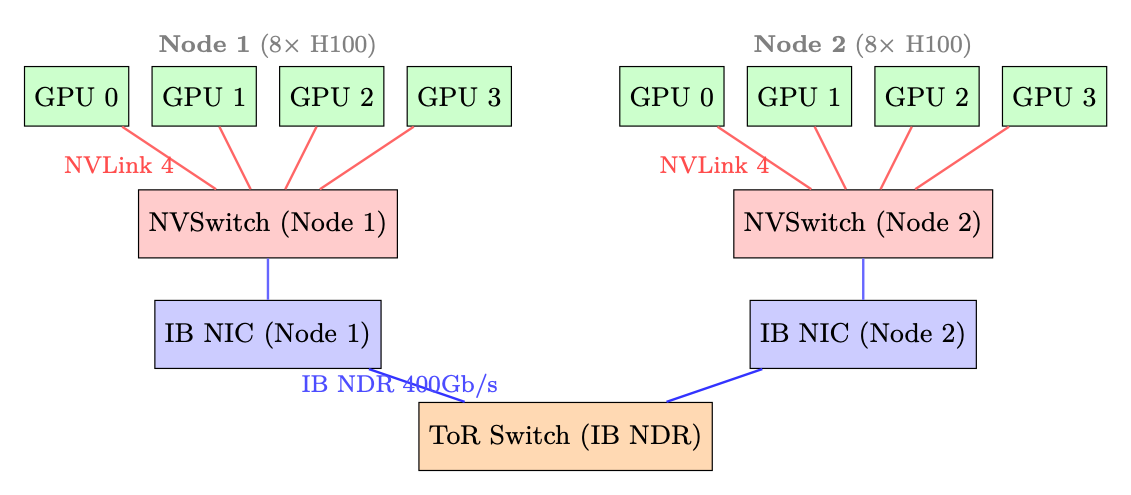
\includegraphics[width=0.85\textwidth]{figures/fig_018_fig18.png}
\caption{两节点 8-GPU 拓扑。节点内：通过 NVSwitch 的 NVLink 4（总计 900 GB/s）。节点间：通过机架顶端交换机的 InfiniBand NDR 400Gb/s。每个节点配有 8 块 IB 网卡（每块 GPU 一块），用于轨道优化 AllReduce。}
\end{figure}

\begin{intuitionbox}[根据带宽选择并行策略]
\begin{itemize}
  % \item \textbf{Tensor Parallelism (TP):} Requires all-reduce every layer -- use only within a node over NVLink. TP=8 is standard for H100 DGX nodes.
  \item \textbf{张量并行（TP）：}每层都需要 all-reduce——仅在节点内通过 NVLink 使用。TP=8 是 H100 DGX 节点的标准。
  % \item \textbf{Pipeline Parallelism (PP):} Point-to-point between stages -- can cross nodes, but adds pipeline bubble overhead. Use when model is too large for TP alone.
  \item \textbf{流水线并行（PP）：}阶段之间的点对点通信——可以跨节点，但会引入流水线气泡开销。当模型大到单靠 TP 装不下时使用。
  % \item \textbf{Data Parallelism (DP):} AllReduce of gradients -- can cross nodes via IB. Scales well with fast IB.
  \item \textbf{数据并行（DP）：}梯度的 AllReduce——可以通过 IB 跨节点。在快速 IB 下扩展性良好。
  % \item \textbf{FSDP/ZeRO:} AllGather + ReduceScatter -- similar to DP but shards optimizer states. Preferred over DP for large models.
  \item \textbf{FSDP/ZeRO：}AllGather + ReduceScatter——类似于 DP 但会分片优化器状态。对于大模型优于 DP。
\end{itemize}
\end{intuitionbox}

\section{vLLM——分页注意力与高吞吐推理}
\label{vllm-pagedattention-and-high-throughput-inference}

% vLLM~\cite{kwon2023efficient} introduced PagedAttention, which borrows the paging abstraction that operating systems use for RAM and applies it to the GPU's KV cache. During LLM inference, the \emph{KV cache} -- the stored key and value tensors for all previous tokens -- is the dominant memory consumer. Managing it efficiently is the central challenge of high-throughput inference.
vLLM~\cite{kwon2023efficient} 引入了分页注意力（PagedAttention），它借鉴操作系统用于管理 RAM 的分页抽象，并将其应用于 GPU 的键值缓存（KV Cache）。在 LLM 推理过程中，\emph{KV cache}——存储了所有先前 token 的 key 和 value 张量——是最大的内存消耗者。高效管理 KV cache 是高吞吐推理的核心挑战。

\subsection{KV cache 碎片化问题}
\label{the-kv-cache-fragmentation-problem}

\begin{keybox}[KV cache 显存计算公式]
% For a model with $L$ layers, $H$ heads, head dimension $d$, and a sequence of $n$ tokens:
对于具有 $L$ 层、$H$ 个头、头维度 $d$、序列长度为 $n$ 个 token 的模型：
\[
\text{KV cache 大小} = 2 \times L \times H \times d \times n \times \text{每元素字节数}
\]
% For Llama-3 70B (BF16): $L=80$, $H=8$ (GQA), $d=128$:
对于 Llama-3 70B（BF16）：$L=80$、$H=8$（GQA）、$d=128$：
\[
= 2 \times 80 \times 8 \times 128 \times n \times 2 = 327{,}680 \times n \text{ bytes}
\]
% At $n=4096$ tokens: $\approx 1.3$ GB per sequence.
当 $n=4096$ token 时：每条序列约 1.3 GB。
\end{keybox}

\begin{intuitionbox}[内部碎片与外部碎片]
% Traditional inference systems pre-allocate a contiguous memory block for each sequence's KV cache, sized to the \emph{maximum possible sequence length}. This causes two types of waste:
传统推理系统会为每条序列的 KV cache 预先分配一块连续内存，大小为\emph{可能的最大序列长度}。这会造成两类浪费：

% \textbf{Internal fragmentation:} A sequence that generates only 500 tokens still holds a block reserved for 4096 tokens. The unused 3596 token slots are wasted.
\textbf{内部碎片：}一条只生成 500 token 的序列仍然占据为 4096 token 预留的块。未使用的 3596 个 token 槽位被浪费。

% \textbf{External fragmentation:} After many sequences complete, the free memory consists of many small non-contiguous gaps. A new long sequence cannot be allocated even if total free memory is sufficient, because no single contiguous block is large enough.
\textbf{外部碎片：}许多序列完成后，剩余空闲内存由许多小的不连续空隙组成。即使总空闲内存足够，新的长序列也无法被分配，因为没有任何一块连续区域足够大。

% In practice, GPU memory utilization with naive allocation is often only 20--40\%.
实际中，朴素分配下的 GPU 显存利用率通常只有 20--40\%。
\end{intuitionbox}

\subsection{分页注意力——为 KV cache 引入虚拟内存}
\label{pagedattention-virtual-memory-for-kv-caches}

% PagedAttention (Kwon et al., 2023) borrows the \emph{paging} abstraction from operating systems. Instead of one contiguous block per sequence, the KV cache is carved into fixed-size \textbf{pages} (blocks), and an indirection table---analogous to a CPU page table---translates each sequence's logical token positions into scattered physical GPU memory addresses.
分页注意力（PagedAttention，Kwon 等，2023）借鉴了操作系统的\emph{分页}抽象。它不再为每条序列分配一块连续内存，而是把 KV cache 切分成固定大小的\textbf{页（page）}（即块），并通过一个间接表——类似 CPU 页表——将每条序列的逻辑 token 位置翻译为分散的物理 GPU 内存地址。

\begin{keybox}[PagedAttention 核心概念]
\begin{itemize}
  % \item \textbf{Block size:} Typically 16 tokens per block (tunable). Each block stores $16 \times 2 \times L \times H \times d$ elements.
  \item \textbf{块大小：}通常每块 16 个 token（可调）。每个块存储 $16 \times 2 \times L \times H \times d$ 个元素。
  % \item \textbf{Block table:} A per-sequence mapping from logical block index to physical block index in the GPU memory pool.
  \item \textbf{块表（Block table）：}每条序列一份的映射，把逻辑块索引映射到 GPU 内存池中的物理块索引。
  % \item \textbf{Physical block pool:} A pre-allocated pool of fixed-size blocks. Allocation is $O(1)$ -- just pop from a free list.
  \item \textbf{物理块池：}预先分配好的固定大小块池。分配为 $O(1)$——只需从空闲列表弹出。
  % \item \textbf{Attention kernel:} Modified to gather KV blocks from non-contiguous physical locations using the block table during attention computation.
  \item \textbf{注意力内核：}做了修改，在注意力计算时使用块表从不连续的物理位置 gather KV 块。
\end{itemize}
\end{keybox}

\begin{examplebox}[块表示例]
% Suppose block size = 4 tokens, and we have two sequences:
假设块大小 = 4 个 token，我们有两条序列：

\begin{itemize}
  % \item Sequence A (7 tokens): logical blocks [0,1] $\to$ physical blocks [3, 7]
  \item 序列 A（7 个 token）：逻辑块 [0,1] $\to$ 物理块 [3, 7]
  % \item Sequence B (5 tokens): logical blocks [0,1] $\to$ physical blocks [1, 5]
  \item 序列 B（5 个 token）：逻辑块 [0,1] $\to$ 物理块 [1, 5]
\end{itemize}

% Physical block 3 holds tokens 0--3 of sequence A. Physical block 7 holds tokens 4--6 of sequence A (partially filled). The attention kernel for sequence A reads from physical blocks 3 and 7 in order, using the block table as an indirection layer.
物理块 3 持有序列 A 的 token 0--3。物理块 7 持有序列 A 的 token 4--6（部分填充）。序列 A 的注意力内核按顺序从物理块 3 和 7 读取，并以块表作为间接层。
\end{examplebox}

\subsection{PagedAttention 的收益}
\label{benefits-of-pagedattention}

\paragraph{近零浪费。}
\label{near-zero-waste.}

% Internal fragmentation is bounded by at most one partially-filled block per sequence (the last block). With block size 16, worst-case waste is 15 tokens per sequence -- negligible. External fragmentation is eliminated because blocks are fixed-size and interchangeable.
内部碎片至多为每条序列一个部分填充块（最后一个块）。当块大小为 16 时，最差浪费为每条序列 15 个 token——可忽略不计。外部碎片被消除，因为块是固定大小、可互换的。

\paragraph{动态分配。}
\label{dynamic-allocation.}

% Blocks are allocated on demand as the sequence grows. No need to know the final sequence length in advance. This is critical for generation, where output length is unknown.
块在序列增长时按需分配。无需预先知道最终序列长度。这对生成任务至关重要，因为输出长度未知。

\paragraph{前缀共享（写时复制）。}
\label{prefix-sharing-copy-on-write.}

% Multiple sequences sharing a common prefix (e.g., a system prompt) can share the \emph{same physical blocks} for that prefix. The block table simply points multiple sequences to the same physical blocks. When a sequence needs to write to a shared block (diverging from the prefix), a copy-on-write is triggered.
多条共享同一前缀（例如同一系统提示）的序列可以\emph{共享相同的物理块}来表示该前缀。块表只需让多条序列指向相同的物理块。当某条序列需要写入共享块（与前缀分叉）时，会触发写时复制（Copy-on-Write）。

\begin{intuitionbox}[前缀共享带来的节约]
% In a chatbot with a 1000-token system prompt serving 128 concurrent users:
在一个拥有 1000-token 系统提示、服务 128 位并发用户的聊天机器人中：

\begin{itemize}
  % \item Without prefix sharing: $128 \times 1000 \times 327{,}680 / 10^9 \approx 42$ GB just for system prompt KV cache
  \item 无前缀共享：仅系统提示 KV cache 就需 $128 \times 1000 \times 327{,}680 / 10^9 \approx 42$ GB
  % \item With prefix sharing: $1 \times 1000 \times 327{,}680 / 10^9 \approx 0.33$ GB
  \item 有前缀共享：$1 \times 1000 \times 327{,}680 / 10^9 \approx 0.33$ GB
  % \item Savings: $\sim$128$\times$ for the shared prefix portion
  \item 节约：共享前缀部分约 128$\times$
\end{itemize}
\end{intuitionbox}

\paragraph{通过 swap 抢占。}
\label{preemption-via-swap.}

% When GPU memory is exhausted, vLLM can \emph{preempt} a sequence by swapping its KV blocks to CPU DRAM (or simply discarding them and recomputing later). This is only feasible because blocks are self-contained and non-contiguous -- swapping a contiguous allocation would require copying the entire buffer.
当 GPU 显存耗尽时，vLLM 可以通过把某条序列的 KV 块换出到 CPU DRAM（或者直接丢弃，之后重新计算）来\emph{抢占}该序列。这之所以可行，是因为块是自包含且非连续的——若是连续分配则需要复制整个缓冲区。

\subsection{连续批处理}
\label{continuous-batching}

% Traditional batching (``static batching``) waits until \emph{all} sequences in a batch finish before starting new ones. If one sequence generates 500 tokens and another generates 10, the GPU is idle for 490 steps on the short sequence. This is extremely wasteful.
传统的批处理（“静态批处理”）会等到一批中\emph{所有}序列都完成后才开始新批次。如果一条序列生成 500 个 token、另一条生成 10 个，那么 GPU 在短序列上有 490 步是空闲的。这极其浪费。

\begin{keybox}[连续批处理（Continuous Batching）]
% Continuous batching (also called iteration-level scheduling) processes one \emph{decode step} at a time. After each step:
连续批处理（Continuous Batching，也叫迭代级调度）一次处理一个\emph{解码步}。每一步之后：

\begin{enumerate}
  % \item Check which sequences have finished (generated EOS token)
  \item 检查哪些序列已完成（生成了 EOS token）
  % \item Remove finished sequences from the batch, freeing their KV blocks
  \item 把已完成的序列从批中移除，释放其 KV 块
  % \item Add new waiting sequences to fill the freed slots
  \item 加入新的等待序列以填补空出的槽位
  % \item Run the next decode step with the updated batch
  \item 在更新后的批上运行下一解码步
\end{enumerate}

% The batch composition changes every step --- sequences join and leave dynamically. This keeps GPU utilization near 100\% and dramatically improves throughput (1.5--3$\times$ over static batching). PagedAttention is essential here: adding/removing sequences mid-batch requires dynamic KV block allocation/deallocation, which is only efficient with paged memory.
批次组成每一步都在变化——序列动态地加入和离开。这让 GPU 利用率接近 100\%，并大幅提升吞吐（相对静态批处理提升 1.5--3$\times$）。PagedAttention 在这里至关重要：在批次中动态添加/移除序列需要动态分配/释放 KV 块，只有在分页内存下才高效。
\end{keybox}

\subsection{vLLM 中的投机解码}
\label{speculative-decoding-integration}

% Speculative decoding uses a small \emph{draft model} (e.g., 1B parameters) to propose $k$ candidate tokens quickly, which the large \emph{target model} verifies in a single forward pass. All tokens up to the first rejection are accepted (expected acceptance: 3--5 tokens per verification step). This yields 2--3$\times$ speedup for latency-sensitive single-sequence generation without any quality loss.
投机解码（Speculative Decoding）使用一个小型\emph{草稿模型}（draft model，例如 1B 参数）快速提出 $k$ 个候选 token，再由大型\emph{目标模型}（target model）在一次前向传播中验证。从第一个被拒绝处之前的所有 token 都会被接受（预期接受数：每次验证 3--5 个 token）。这为延迟敏感的单序列生成带来 2--3$\times$ 提速，且无质量损失。

% vLLM integrates speculative decoding with PagedAttention:
vLLM 将投机解码与 PagedAttention 集成：

\begin{itemize}
  % \item Draft tokens are allocated speculative KV blocks
  \item 草稿 token 被分配投机性 KV 块
  % \item On rejection, speculative blocks are freed (cheap with paged allocation)
  \item 拒绝时，投机块被释放（在分页分配下成本极低）
  % \item On acceptance, speculative blocks are promoted to the main sequence
  \item 接受时，投机块被提升为主序列的一部分
  % \item The block table update is $O(k)$ -- just updating a few table entries
  \item 块表更新为 $O(k)$——只需更新少量表项
\end{itemize}

\subsection{具体显存节约——大规模 70B 模型}
\label{concrete-memory-savings-70b-model-at-scale}

\begin{examplebox}[显存预算——70B BF16 推理]
% \textbf{Setup:} Llama-3 70B, BF16, single A100 80GB node (8 GPUs, tensor parallel).
\textbf{设定：}Llama-3 70B，BF16，单个 A100 80GB 节点（8 GPU，张量并行）。

% \textbf{Model weights:} $70 \times 10^9 \times 2$ bytes $= 140$ GB $\div$ 8 GPUs $= 17.5$ GB/GPU.
\textbf{模型权重：}$70 \times 10^9 \times 2$ 字节 $= 140$ GB $\div$ 8 GPU $= 17.5$ GB/GPU。

% \textbf{Remaining for KV cache:} $80 - 17.5 - 3$ (overhead) $= 59.5$ GB/GPU.
\textbf{KV cache 可用部分：}$80 - 17.5 - 3$（开销）$= 59.5$ GB/GPU。

% \textbf{KV cache per token per GPU} (with TP=8, each GPU holds $1/8$ of heads): $2 \times 80 \times 1 \times 128 \times 2 = 40{,}960$ bytes $\approx 40$ KB/token.
\textbf{每块 GPU 每 token 的 KV cache}（TP=8 时每块 GPU 持有 $1/8$ 的头）：$2 \times 80 \times 1 \times 128 \times 2 = 40{,}960$ 字节 $\approx 40$ KB/token。

% \textbf{Max tokens in KV cache:} $59.5 \times 10^9 / 40{,}960 \approx 1.45$ million tokens.
\textbf{KV cache 最大 token 数：}$59.5 \times 10^9 / 40{,}960 \approx 145$ 万 token。

% \textbf{With 128 concurrent sequences of 4096 tokens each:} $128 \times 4096 = 524{,}288$ tokens -- well within budget.
\textbf{当 128 条并发序列每条 4096 个 token 时：}$128 \times 4096 = 524{,}288$ 个 token——完全在预算之内。

% \textbf{Without PagedAttention} (pre-allocating max length 4096 for each): Same math, but fragmentation wastes $\sim$50\% on average $\to$ only 64 sequences fit.
\textbf{若不使用 PagedAttention}（为每条序列预分配最大长度 4096）：同样的计算，但碎片化平均浪费约 50\% $\to$ 只能容纳 64 条序列。
\end{examplebox}

\begin{warningbox}[块大小的权衡]
% Larger block sizes reduce the overhead of the block table and improve memory access locality (fewer scattered reads). Smaller block sizes reduce internal fragmentation and enable finer-grained prefix sharing. vLLM defaults to 16 tokens/block, which is a good balance. For very long sequences (100K+ tokens), larger blocks (32--64) may be preferable.
更大的块大小可减少块表开销，并提高内存访问局部性（更少的分散读取）。更小的块大小可减少内部碎片，并支持更细粒度的前缀共享。vLLM 默认每块 16 个 token，是一个不错的平衡。对于非常长的序列（10 万+ token），更大的块（32--64）可能更合适。
\end{warningbox}

\subsection{vLLM：端到端系统}
\label{vllm-end-to-end-system}

% vLLM wraps PagedAttention inside a full serving stack: continuous batching, prefix caching, speculative decoding, and tensor-parallel model sharding all work together to maximize throughput per GPU dollar.
vLLM 将 PagedAttention 封装在一整套服务栈中：连续批处理（Continuous Batching）、前缀缓存（Prefix Caching）、投机解码（Speculative Decoding）以及张量并行的模型分片协同工作，最大化每美元 GPU 的吞吐。

\subsection{架构总览}
\label{architecture-overview}

\begin{figure}[ht!]
\centering
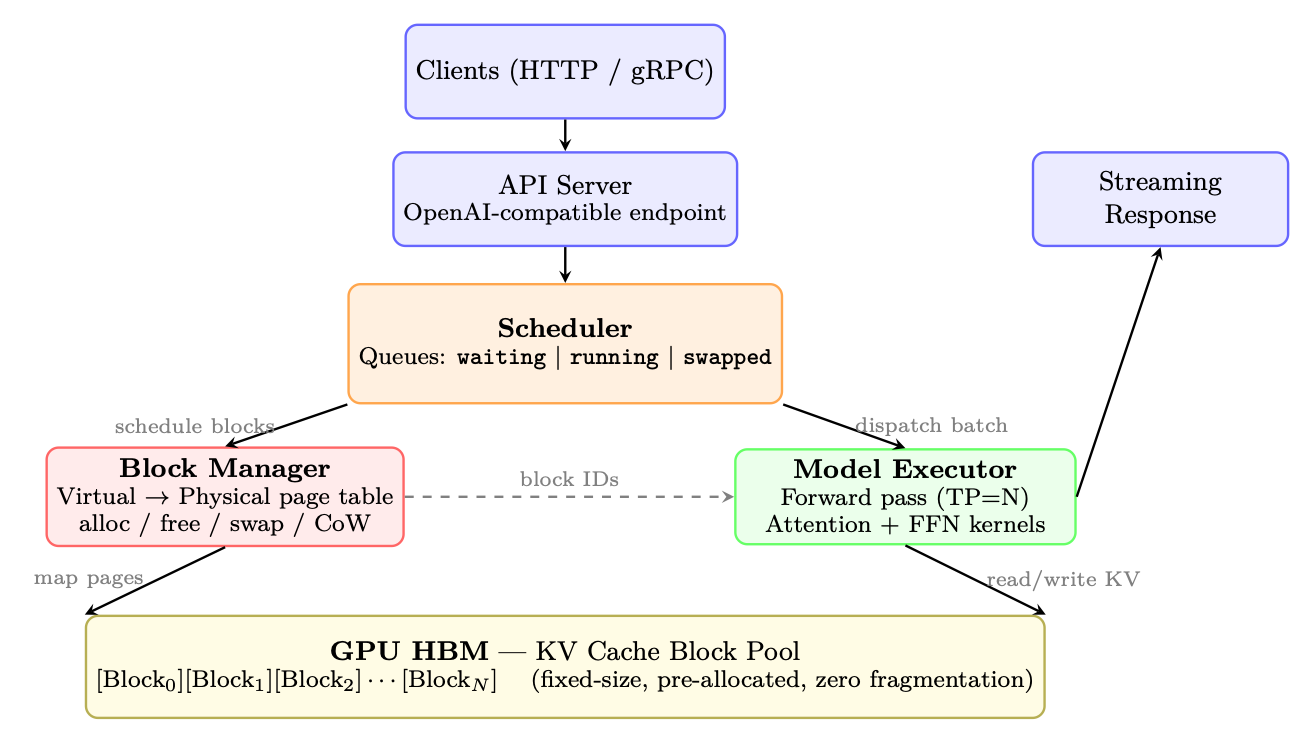
\includegraphics[width=0.85\textwidth]{figures/fig_019_fig19.png}
\caption{vLLM 架构：请求自上而下流动。Scheduler 管理准入与抢占，Block Manager 负责虚拟到物理 KV cache 映射（像操作系统页表一样），Model Executor 在 GPU HBM 中从预分配的块池读取数据并执行批量推理。}
\end{figure}

\subsection{核心组件}
\label{core-components}

\begin{itemize}
  % \item \textbf{API Server}: Accepts OpenAI-compatible requests (completions, chat). Tokenizes inputs and creates ``sequence groups'' (for beam search or multiple samples).
  \item \textbf{API Server}：接收 OpenAI 兼容的请求（completions、chat）。对输入进行 tokenize，并创建“序列组（sequence groups）”（用于 beam search 或多样本）。
  % \item \textbf{Scheduler}: The brain of vLLM. Maintains three queues:
  \item \textbf{Scheduler}：vLLM 的大脑。维护三个队列：

\begin{itemize}
  % \item \texttt{waiting}: New requests not yet started (prefill pending)
  \item \texttt{waiting}：尚未开始的新请求（等待 prefill）
  % \item \texttt{running}: Actively generating tokens (decode phase)
  \item \texttt{running}：正在生成 token（decode 阶段）
  % \item \texttt{swapped}: Preempted requests whose KV cache was offloaded to CPU
  \item \texttt{swapped}：被抢占、KV cache 已卸载到 CPU 的请求
\end{itemize}

% Each iteration, the scheduler decides which requests to run based on available GPU memory blocks.
每次迭代，调度器根据可用 GPU 内存块决定运行哪些请求。
  % \item \textbf{Block Manager}: Implements the virtual memory abstraction for KV caches. Maps logical blocks (per-sequence) to physical blocks (in GPU memory pool). Handles:
  \item \textbf{Block Manager}：为 KV cache 实现虚拟内存抽象。将逻辑块（按序列）映射到物理块（GPU 内存池中）。负责处理：

\begin{itemize}
  % \item Allocation (new tokens generated $\rightarrow$ new blocks needed)
  \item 分配（生成新 token $\rightarrow$ 需要新块）
  % \item Copy-on-write (for beam search: multiple beams share prefix blocks, copy only on divergence)
  \item 写时复制（Copy-on-Write）（用于 beam search：多 beam 共享前缀块，仅在分叉时复制）
  % \item Swap (GPU $\leftrightarrow$ CPU migration when preempting/resuming)
  \item Swap（抢占/恢复时在 GPU $\leftrightarrow$ CPU 之间迁移）
  % \item Prefix caching (reuse cached blocks when prompts share common prefixes)
  \item 前缀缓存（Prefix Caching）（当 prompt 共享相同前缀时复用已缓存块）
\end{itemize}
  % \item \textbf{Model Executor}: Runs the actual LLM forward pass. Manages tensor parallelism across GPUs, dispatches attention kernels that read from paged KV cache blocks.
  \item \textbf{Model Executor}：执行实际的 LLM 前向传播。管理跨 GPU 的张量并行，调度从分页 KV cache 块读取的注意力内核。
  % \item \textbf{KV Cache Pool}: Pre-allocated GPU memory divided into fixed-size blocks (default: 16 tokens $\times$ num\_heads $\times$ head\_dim $\times$ 2 bytes per block). No dynamic allocation at runtime $\rightarrow$ zero fragmentation.
  \item \textbf{KV Cache Pool}：预分配的 GPU 内存，划分为固定大小的块（默认每块 16 token $\times$ num\_heads $\times$ head\_dim $\times$ 2 字节）。运行时无动态分配 $\rightarrow$ 零碎片。
\end{itemize}

\subsection{请求生命周期（端到端流程）}
\label{request-lifecycle-end-to-end-flow}

\begin{enumerate}
  % \item \textbf{Arrival}: Client sends prompt. API server tokenizes it, creates a \texttt{SequenceGroup}, places it in the \texttt{waiting} queue.
  \item \textbf{到达}：客户端发送 prompt。API server 将其 tokenize，创建一个 \texttt{SequenceGroup}，放入 \texttt{waiting} 队列。
  % \item \textbf{Scheduling}: At each step, the scheduler runs:
  \item \textbf{调度}：每一步，调度器执行：

\begin{enumerate}
  % \item Check if any \texttt{swapped} sequences can be resumed (enough free blocks).
  \item 检查是否有 \texttt{swapped} 序列可以恢复（有足够空闲块）。
  % \item Check if any \texttt{waiting} sequences can start prefill (enough blocks for the full prompt).
  \item 检查是否有 \texttt{waiting} 序列可以开始 prefill（有足够块容纳完整 prompt）。
  % \item Budget remaining blocks across \texttt{running} sequences (need 1 new block per sequence per step if current block is full).
  \item 在 \texttt{running} 序列之间预算剩余块（若当前块已满，每条序列每步需要 1 个新块）。
  % \item If over budget: \textbf{preempt} lowest-priority running sequences (swap KV to CPU or recompute later).
  \item 如果超出预算：\textbf{抢占}优先级最低的运行中序列（把 KV 换出到 CPU 或之后重新计算）。
\end{enumerate}
  % \item \textbf{Prefill} (first iteration for a request): The entire prompt is processed in one forward pass. KV cache is computed for all prompt tokens and stored in allocated blocks. This is compute-bound (large batch of tokens).
  \item \textbf{Prefill}（请求的第一次迭代）：整个 prompt 在一次前向传播中被处理。所有 prompt token 的 KV cache 被计算并存入已分配的块。这是计算密集（Compute-Bound）的（大批 token）。
  % \item \textbf{Decode} (subsequent iterations): One new token generated per sequence per step. All running sequences are batched together (continuous batching). This is memory-bound (reads full KV cache, generates 1 token).
  \item \textbf{Decode}（后续迭代）：每条序列每步生成一个新 token。所有运行中的序列被一起 batch（连续批处理）。这是内存密集（Memory-Bound）的（读取完整 KV cache，生成 1 个 token）。
  % \item \textbf{Block Allocation}: After each decode step, if the last block for a sequence is full, the Block Manager allocates a new physical block and maps it to the next logical block.
  \item \textbf{块分配}：每个 decode 步后，如果某条序列的最后一个块已满，Block Manager 分配一个新的物理块并将其映射到下一逻辑块。
  % \item \textbf{Completion}: When a sequence hits EOS or max length, it's removed from \texttt{running}. Its physical blocks are freed immediately $\rightarrow$ available for other sequences. Response is streamed back to client.
  \item \textbf{完成}：当一条序列遇到 EOS 或达到最大长度时，它会从 \texttt{running} 中移除。其物理块立即被释放 $\rightarrow$ 可供其他序列使用。响应被流式回传给客户端。
\end{enumerate}

\subsection{前缀缓存（自动 Prompt 缓存）}
\label{prefix-caching-automatic-prompt-caching}

% When multiple requests share a common prefix (system prompt, few-shot examples):
当多个请求共享相同前缀（系统 prompt、few-shot 示例）时：

\begin{enumerate}
  % \item Hash the token content of each logical block.
  \item 对每个逻辑块的 token 内容计算哈希。
  % \item On new request arrival, check if any prefix blocks are already in the cache.
  \item 新请求到达时，检查是否有前缀块已在缓存中。
  % \item If hit: skip prefill for those tokens, directly reuse physical KV blocks. Time-to-first-token drops dramatically.
  \item 命中时：跳过这些 token 的 prefill，直接复用物理 KV 块。首 token 延迟（Time-to-first-token）大幅下降。
  % \item Eviction: LRU policy. Cached blocks are freed only when memory pressure requires it.
  \item 驱逐：LRU 策略。缓存块仅在内存压力需要时才被释放。
\end{enumerate}

% \textbf{Impact}: For chat applications with long system prompts (2K+ tokens shared across all users), prefix caching reduces TTFT by 60--80\%.
\textbf{影响}：对于具有长系统提示（2K+ token、所有用户共享）的聊天应用，前缀缓存可降低 TTFT 60--80\%。

\subsection{vLLM 中的引导（受约束）解码}
\label{sec:vllm-guided-decoding}

% vLLM natively supports constrained decoding (Section~\ref{sec:constrained-decoding}) through pluggable backends, enabling \emph{guaranteed} structured output at serving time with minimal performance overhead.
vLLM 通过可插拔的后端原生支持受约束解码（参见 Section~\ref{sec:constrained-decoding}），可以在服务期间以极小的性能开销\emph{保证}结构化输出。

\paragraph{支持的约束类型。}
\label{supported-constraint-types.}

% The OpenAI-compatible API accepts constraints via the \texttt{guided\_*} parameters or the \texttt{response\_format} field:
OpenAI 兼容 API 通过 \texttt{guided\_*} 参数或 \texttt{response\_format} 字段接受约束：

\begin{lstlisting}[style=pythonstyle]
from openai import OpenAI
client = OpenAI(base_url="http://localhost:8000/v1")

# --- JSON Schema 约束 ---
response = client.chat.completions.create(
    model="meta-llama/Llama-3-70B-Instruct",
    messages=[{"role": "user",
               "content": "Extract: name, age, city from: "
                          "'John is 30 and lives in NYC'"}],
    extra_body={
        "guided_json": {
            "type": "object",
            "properties": {
                "name": {"type": "string"},
                "age": {"type": "integer"},
                "city": {"type": "string"}
            },
            "required": ["name", "age", "city"]
        }
    }
)
# 输出保证是符合该 schema 的合法 JSON

# --- 正则表达式约束 ---
response = client.completions.create(
    model="meta-llama/Llama-3-70B-Instruct",
    prompt="Generate an IPv4 address: ",
    extra_body={
        "guided_regex": r"\d{1,3}\.\d{1,3}\.\d{1,3}\.\d{1,3}"
    }
)

# --- 选项约束 ---
response = client.completions.create(
    model="meta-llama/Llama-3-70B-Instruct",
    prompt="Sentiment: ",
    extra_body={"guided_choice": ["positive", "negative", "neutral"]}
)
\end{lstlisting}

\paragraph{后端架构。}
\label{backend-architecture.}

% vLLM delegates mask computation to a backend engine:
vLLM 将掩码计算委托给后端引擎：

\begin{itemize}
  % \item \textbf{XGrammar} (default since v0.7): Pushdown-automaton engine supporting JSON schemas, regexes, and arbitrary EBNF grammars. Fastest for complex schemas due to efficient C++ core.
  \item \textbf{XGrammar}（自 v0.7 起为默认）：基于下推自动机的引擎，支持 JSON schema、正则和任意 EBNF 语法。得益于高效的 C++ 核心，对复杂 schema 而言最快。
  % \item \textbf{Outlines}~\cite{willard2023outlines}: FSM-based; supports JSON and regex. Used as fallback when XGrammar is unavailable.
  \item \textbf{Outlines}~\cite{willard2023outlines}：基于 FSM；支持 JSON 和正则。在 XGrammar 不可用时作为回退方案。
\end{itemize}

% The mask is applied \emph{after} the model's forward pass produces logits and \emph{before} sampling---adding $<$1 ms per step in practice, since the FSM/PDA state transition and precomputed index lookup are $O(1)$.
掩码在模型前向传播产生 logits \emph{之后}、采样\emph{之前}施加——实际中每步只增加不到 1 ms，因为 FSM/PDA 状态转移和预先计算的索引查找均为 $O(1)$。

\paragraph{性能影响。}
\label{performance-impact.}

% Because the constraint only masks logits (no recomputation of attention or FFN), throughput loss is negligible ($<$2\% in benchmarks). The main cost is \emph{compilation} of the schema into an FSM/PDA index, which takes 0.5--5 s depending on schema complexity. vLLM caches compiled schemas across requests, so this cost is paid once per unique schema.
由于约束仅对 logits 进行掩码（不重新计算 attention 或 FFN），吞吐损失可忽略（基准测试中 $<$2\%）。主要成本来自把 schema \emph{编译}成 FSM/PDA 索引，耗时 0.5--5 秒，取决于 schema 复杂度。vLLM 会跨请求缓存已编译的 schema，因此每个独特 schema 只需支付一次成本。

\begin{warningbox}[结构化输出 $\neq$ 正确输出]
% Constrained decoding guarantees the output is \emph{syntactically} valid (parses as JSON, matches the schema types). It does \emph{not} guarantee \emph{semantic} correctness---the model may still hallucinate values that parse correctly but are factually wrong. Always validate business logic downstream.
受约束解码保证输出\emph{语法上}有效（能解析为 JSON、符合 schema 的类型）。但它\emph{不}保证\emph{语义上}的正确性——模型仍可能产生能成功解析但事实错误的幻觉值。务必在下游验证业务逻辑。
\end{warningbox}

\begin{table}[ht!]
\centering\small
\caption{vLLM 与其他方案的性能对比（70B 模型，A100 $\times$ 4，TP=4）。}
% Widen the right ("原因") column so the Chinese explanation doesn't wrap.
% Weighted X trick from tabularx: the three X columns' \hsize values must
% sum to 3 (to preserve total width). Give the left two 0.7 each and the
% right one 1.6, then re-apply linebreak parameters that \hsize resets.
\noindent\begin{tabularx}{\linewidth}{@{}l Z{0.61} Z{0.6} Z{1.79}@{}}
\toprule
\textbf{指标} & \textbf{vLLM} & \textbf{HF Generate} & \textbf{原因} \\
\midrule
吞吐（tok/s） & 2,500--4,000 & 300--600 & 连续批处理 + PagedAttention \\
显存利用率 & 90--95\% & 50--60\% & 零碎片，动态块分配 \\
最大并发序列数 & 200--500 & 16--32 & 分页 KV 消除每序列预留 \\
首 token 延迟 & 100--300ms & 500--2000ms & 对重复系统提示启用前缀缓存 \\
\bottomrule
\end{tabularx}
\end{table}

% \chapter{Introduction to Reinforcement Learning}
\chapter{强化学习导论}
\label{sec:rl}

% Reinforcement Learning (RL) is a paradigm where an \textbf{agent} learns to make sequential decisions by interacting with an \textbf{environment}, receiving \textbf{rewards} as feedback, and optimizing its \textbf{policy} to maximize cumulative reward over time~\cite{sutton2018reinforcement}. Unlike supervised learning (which requires labeled input-output pairs), RL discovers optimal behavior through \emph{trial and error}.
强化学习（Reinforcement Learning，RL）是一种范式，其中\textbf{智能体（agent）}通过与\textbf{环境（environment）}交互、接收\textbf{奖励（rewards）}作为反馈，并优化其\textbf{策略（policy）}以最大化长期累积奖励来学习做出序贯决策~\cite{sutton2018reinforcement}。与监督学习（需要带标签的输入-输出对）不同，RL 通过\emph{试错（trial and error）}来发现最优行为。

\begin{figure}[ht!]
\centering
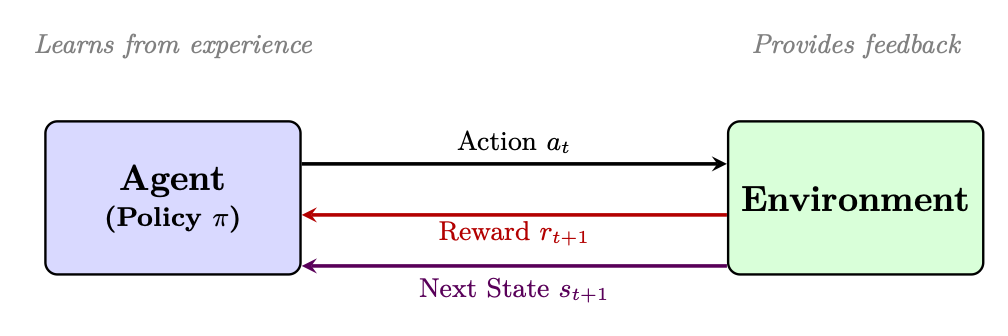
\includegraphics[width=0.85\textwidth]{figures/fig_020_fig20.png}
% \caption{Reinforcement Learning overview: an agent interacts with an environment, receiving rewards as feedback and updating its policy through trial and error. Unlike supervised learning which learns from labeled pairs, RL learns what to do by maximizing reward through experience.}
\caption{强化学习概览：智能体与环境交互，接收奖励作为反馈，并通过试错更新其策略。与从带标签数据对学习的监督学习不同，RL 通过经验最大化奖励来学习应当做什么。}
\end{figure}

% \section{The Markov Decision Process (MDP)}
\section{马尔可夫决策过程（Markov Decision Process，MDP）}
\label{the-markov-decision-process-mdp}

% An MDP is a 5-tuple $(S, A, P, R, \gamma)$:
MDP 是一个五元组 $(S, A, P, R, \gamma)$：

\begin{itemize}
  % \item $S$: State space --- all possible configurations of the environment
  \item $S$：状态空间——环境所有可能的配置
  % \item $A$: Action space --- all actions available to the agent
  \item $A$：动作空间——智能体可用的所有动作
  % \item $P(s'|s, a)$: Transition function --- probability of reaching state $s'$ from state $s$ after taking action $a$
  \item $P(s'|s, a)$：转移函数——在状态 $s$ 下采取动作 $a$ 后到达状态 $s'$ 的概率
  % \item $R(s, a, s')$: Reward function --- immediate scalar feedback for a transition
  \item $R(s, a, s')$：奖励函数——一次状态转移获得的即时标量反馈
  % \item $\gamma \in [0, 1]$: Discount factor --- how much future rewards are valued relative to immediate ones
  \item $\gamma \in [0, 1]$：折扣因子——未来奖励相对于即时奖励的权重
\end{itemize}

% \textbf{The Markov Property}: The future depends only on the current state, not the history:
\textbf{马尔可夫性质（Markov Property）}：未来只依赖于当前状态，而不依赖于历史：
\[
P(s_{t+1} | s_t, a_t, s_{t-1}, a_{t-1}, \ldots) = P(s_{t+1} | s_t, a_t)
\]
% This makes the problem tractable.
这一性质使问题变得可处理。

% \begin{intuitionbox}[Agent-Environment Interaction Loop]
\begin{intuitionbox}[智能体-环境交互循环]
% At each time step $t$:
在每个时间步 $t$：

\begin{enumerate}
  % \item Agent observes state $s_t$
  \item 智能体观察状态 $s_t$
  % \item Agent selects action $a_t$ according to policy $\pi(a|s)$
  \item 智能体根据策略 $\pi(a|s)$ 选择动作 $a_t$
  % \item Environment transitions to $s_{t+1} \sim P(\cdot|s_t, a_t)$
  \item 环境转移到 $s_{t+1} \sim P(\cdot|s_t, a_t)$
  % \item Agent receives reward $r_t = R(s_t, a_t, s_{t+1})$
  \item 智能体接收奖励 $r_t = R(s_t, a_t, s_{t+1})$
  % \item Repeat until terminal state or horizon $T$
  \item 重复直到终止状态或时间步上限 $T$
\end{enumerate}
\end{intuitionbox}

% \section{Core Concepts and Definitions}
\section{核心概念与定义}
\label{core-concepts-and-definitions}

% \textbf{Policy} $\pi(a|s)$: A mapping from states to action probabilities. Deterministic: $a = \pi(s)$. Stochastic: $a \sim \pi(\cdot|s)$.
\textbf{策略（Policy）} $\pi(a|s)$：从状态到动作概率的映射。确定性策略：$a = \pi(s)$；随机性策略：$a \sim \pi(\cdot|s)$。

% \textbf{Return} (cumulative discounted reward):
\textbf{回报（Return）}（累积折扣奖励）：
\begin{equation}
G_t = \sum_{k=0}^{\infty} \gamma^k r_{t+k} = r_t + \gamma r_{t+1} + \gamma^2 r_{t+2} + \cdots
\end{equation}

% \textbf{Value Function} (expected return from state $s$ under policy $\pi$):
\textbf{价值函数（Value Function）}（在策略 $\pi$ 下从状态 $s$ 出发的期望回报）：
\begin{equation}
V^\pi(s) = \mathbb{E}_\pi\left[G_t \mid s_t = s\right] = \mathbb{E}_\pi\left[\sum_{k=0}^{\infty} \gamma^k r_{t+k} \mid s_t = s\right]
\end{equation}

% \textbf{Action-Value Function} (expected return from state $s$, taking action $a$, then following $\pi$):
\textbf{动作价值函数（Action-Value Function）}（从状态 $s$ 出发、采取动作 $a$、其后遵循 $\pi$ 的期望回报）：
\begin{equation}
Q^\pi(s, a) = \mathbb{E}_\pi\left[G_t \mid s_t = s, a_t = a\right]
\end{equation}

% \textbf{Advantage Function} (how much better action $a$ is compared to average):
\textbf{优势函数（Advantage Function）}（动作 $a$ 相对于平均水平好多少）：
\begin{equation}
A^\pi(s, a) = Q^\pi(s, a) - V^\pi(s)
\end{equation}

% \textbf{Bellman Equations} (recursive relationship):
\textbf{贝尔曼方程（Bellman Equations）}（递归关系）：
\begin{align}
V^\pi(s) &= \sum_a \pi(a|s) \sum_{s'} P(s'|s,a)\left[R(s,a,s') + \gamma V^\pi(s')\right] \\
Q^\pi(s,a) &= \sum_{s'} P(s'|s,a)\left[R(s,a,s') + \gamma \sum_{a'} \pi(a'|s') Q^\pi(s', a')\right]
\end{align}

% \begin{keybox}[Optimal Policy and Bellman Optimality]
\begin{keybox}[最优策略与贝尔曼最优性]
% The optimal policy $\pi^*$ satisfies:
最优策略 $\pi^*$ 满足：
\begin{equation}
V^*(s) = \max_a \sum_{s'} P(s'|s,a)\left[R(s,a,s') + \gamma V^*(s')\right]
\end{equation}

\begin{equation}
Q^*(s,a) = \sum_{s'} P(s'|s,a)\left[R(s,a,s') + \gamma \max_{a'} Q^*(s', a')\right]
\end{equation}
% Once $Q^*$ is known, the optimal policy is simply: $\pi^*(s) = \arg\max_a Q^*(s,a)$.
一旦得到 $Q^*$，最优策略就直接是：$\pi^*(s) = \arg\max_a Q^*(s,a)$。
\end{keybox}

\newpage
% \section{Taxonomy of RL Methods}
\section{强化学习方法的分类}
\label{taxonomy-of-rl-methods}

% Reinforcement learning algorithms can be classified along several axes. Understanding this taxonomy helps select the right approach for a given problem.
强化学习算法可以从多个维度进行分类。理解这一分类体系有助于针对特定问题选择合适的方法。

\begin{figure}[ht!]
\centering
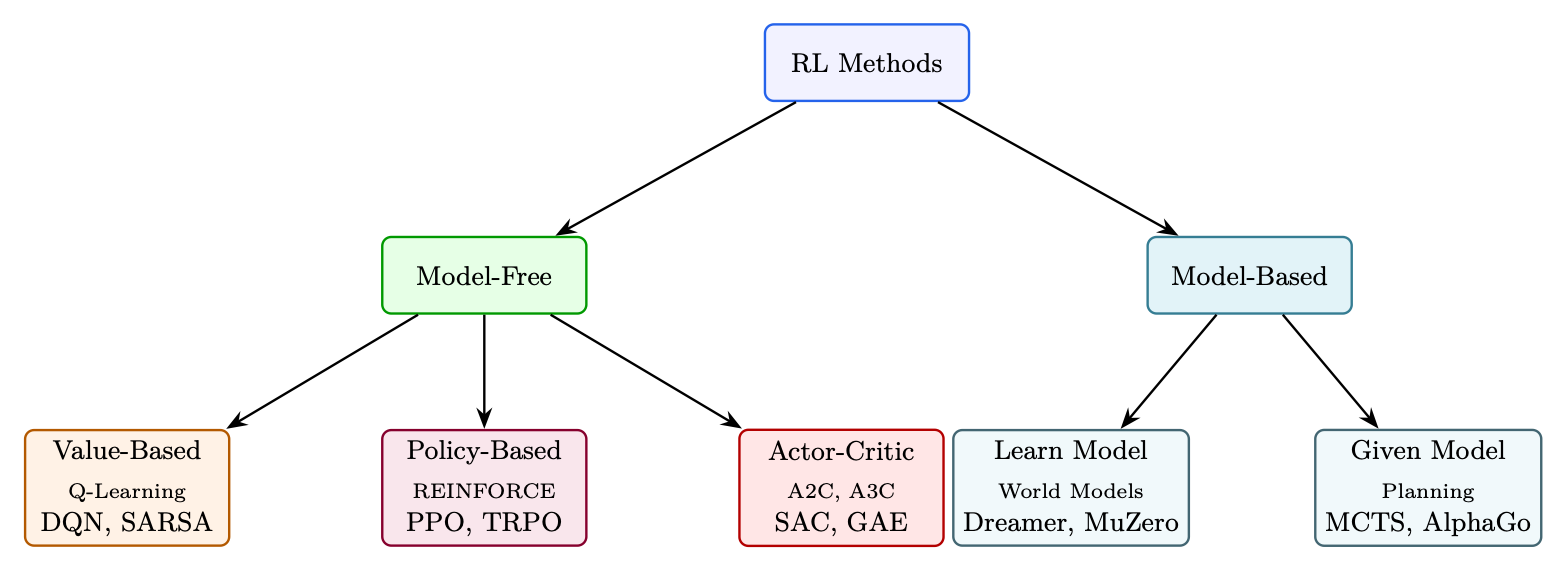
\includegraphics[width=0.85\textwidth]{figures/fig_021_fig21.png}
\end{figure}

% \begin{keybox}[Key Taxonomy Distinctions]
\begin{keybox}[关键分类区分]
% \textbf{Model-Free vs Model-Based}:
\textbf{无模型（Model-Free） vs 基于模型（Model-Based）}：

\begin{itemize}
  % \item \textbf{Model-Free}: Learn policy or value function directly from experience. No knowledge of environment dynamics. Most practical for LLMs (language dynamics are intractable to model).
  \item \textbf{Model-Free}：直接从交互经验中学习策略或价值函数；无需建模环境的转移机制。对 LLM 最实用（语言的转移机制难以建模）。
  % \item \textbf{Model-Based}: Learn or use a model of environment transitions $P(s'|s,a)$. Can plan ahead. More sample-efficient but requires accurate model.
  \item \textbf{Model-Based}：学习或使用环境转移模型 $P(s'|s,a)$。可以提前规划。样本效率更高，但需要准确的模型。
\end{itemize}

% \textbf{Value-Based vs Policy-Based}:
\textbf{基于价值（Value-Based） vs 基于策略（Policy-Based）}：

\begin{itemize}
  % \item \textbf{Value-Based}: Learn $Q(s,a)$ or $V(s)$, derive policy as $\arg\max_a Q(s,a)$. Works well for discrete, small action spaces (e.g., Atari). Struggles with continuous/large action spaces.
  \item \textbf{Value-Based}：学习 $Q(s,a)$ 或 $V(s)$，并通过 $\arg\max_a Q(s,a)$ 得到策略。适合离散、小规模动作空间（如 Atari），在连续或大规模动作空间上表现不佳。
  % \item \textbf{Policy-Based}: Directly parameterize and optimize $\pi_\theta(a|s)$. Natural for continuous/high-dimensional action spaces. Essential for LLMs (vocabulary = 32K--128K actions).
  \item \textbf{Policy-Based}：直接参数化并优化 $\pi_\theta(a|s)$。天然适合连续或高维动作空间，对 LLM 至关重要（词表 = 32K--128K 个动作）。
  % \item \textbf{Actor-Critic}: Combine both --- policy (actor) proposes actions, value function (critic) evaluates them. PPO for LLMs is actor-critic.
  \item \textbf{Actor-Critic}：两者结合——策略（actor）提议动作，价值函数（critic）评估动作。用于 LLM 的 PPO 即属于 actor-critic 方法。
\end{itemize}

% \textbf{On-Policy vs Off-Policy}:
\textbf{同策略（On-Policy） vs 异策略（Off-Policy）}：

\begin{itemize}
  % \item \textbf{On-Policy}: Learn from data generated by the \emph{current} policy. Must regenerate data after each update. Examples: REINFORCE, PPO, A2C. More stable but less sample-efficient.
  \item \textbf{On-Policy}：从\emph{当前}策略生成的数据中学习。每次更新后必须重新生成数据。例如：REINFORCE、PPO、A2C。更稳定但样本效率较低。
  % \item \textbf{Off-Policy}: Learn from data generated by \emph{any} policy (including old versions or other agents). Can reuse past experience. Examples: Q-Learning, DQN, SAC. More sample-efficient but harder to stabilize.
  \item \textbf{Off-Policy}：从\emph{任意}策略生成的数据中学习（包括旧版本或其他智能体）。可以复用过往经验。例如：Q-Learning、DQN、SAC。样本效率高但更难稳定。
\end{itemize}
\end{keybox}

% \section{Temporal Difference (TD) Learning}
\section{时序差分（Temporal Difference，TD）学习}
\label{temporal-difference-td-learning}

% TD learning~\cite{sutton1988learning} bootstraps --- it updates value estimates using other value estimates, without waiting for the full episode to end.
TD 学习~\cite{sutton1988learning}采用自举（bootstrap）思想——它使用其他价值估计来更新价值估计，无需等待完整 episode 结束。

% \subsection{Understanding TD Error: ``Surprise'' as a Learning Signal}
\subsection{理解 TD 误差：以「惊讶」作为学习信号}
\label{understanding-td-error-surprise-as-a-learning-signal}

% \textbf{TD error} measures the discrepancy between an agent's \textbf{current estimate} of future reward and a \textbf{newly updated estimate} after taking one step. Put simply, it is the difference between what the agent \emph{thought} would happen and what \emph{actually} happened plus what it expects next. It represents the agent's ``surprise.''
\textbf{TD 误差（TD Error）}衡量智能体对未来奖励的\textbf{当前估计}与采取一步后\textbf{新估计}之间的差异。简单来说，就是智能体\emph{原本以为}会发生的事，与\emph{实际}发生的事加上对未来的新预期之间的差。它代表了智能体的「惊讶」。

% \begin{examplebox}[Intuition: The Driving Analogy]
\begin{examplebox}[直觉：开车类比]
% Imagine you are driving home and expect the drive to take 30 minutes.
设想你正在开车回家，预计需要 30 分钟。

\begin{itemize}
  % \item \textbf{The prediction}: 30 minutes total.
  \item \textbf{预测}：总共 30 分钟。
  % \item \textbf{The reality shift}: After 10 minutes, you hit unexpected road construction. Your GPS updates, saying you now have 35 minutes left.
  \item \textbf{现实变化}：10 分钟后，你遇到意外的道路施工。GPS 更新提示，你还需要 35 分钟。
  % \item \textbf{The TD Error}: Total expected time is now 45 minutes (10 elapsed + 35 remaining). The difference between new estimate (45 min) and old estimate (30 min) is a \textbf{+15 minute TD error}. You use this ``surprise'' to change your route next time.
  \item \textbf{TD 误差}：总预期时间现在是 45 分钟（已过 10 分钟 + 剩余 35 分钟）。新估计（45 分钟）与旧估计（30 分钟）之差就是 \textbf{+15 分钟的 TD 误差}。你下次会用这个「惊讶」来调整路线。
\end{itemize}

% A \textbf{positive TD error} means the outcome was better than expected $\rightarrow$ boost this state's value.\\
\textbf{正的 TD 误差}意味着结果好于预期 $\rightarrow$ 提升该状态的价值。\\

% A \textbf{negative TD error} means it was worse than expected $\rightarrow$ lower this state's value.
\textbf{负的 TD 误差}意味着结果差于预期 $\rightarrow$ 降低该状态的价值。
\end{examplebox}

% \subsection{The TD Error Formula}
\subsection{TD 误差公式}
\label{the-td-error-formula}

\begin{equation}
\boxed{\delta_t = R_{t+1} + \gamma V(S_{t+1}) - V(S_t)}
\end{equation}

\begin{itemize}
  % \item $R_{t+1}$: The \textbf{immediate reward} received after taking an action.
  \item $R_{t+1}$：采取动作后获得的\textbf{即时奖励}。
  % \item $\gamma V(S_{t+1})$: The estimated \textbf{discounted value} of the next state (what the agent expects to get from the next state onward, scaled by discount factor $\gamma$).
  \item $\gamma V(S_{t+1})$：下一个状态的估计\textbf{折扣价值}（智能体从下一个状态起预期获得的回报，按折扣因子 $\gamma$ 缩放）。
  % \item $V(S_t)$: The \textbf{original estimate} of the current state's value.
  \item $V(S_t)$：当前状态价值的\textbf{原始估计}。
\end{itemize}

% The combined term $(R_{t+1} + \gamma V(S_{t+1}))$ is called the \textbf{TD Target}. Therefore:
组合项 $(R_{t+1} + \gamma V(S_{t+1}))$ 被称为 \textbf{TD 目标（TD Target）}。因此：
\begin{equation}
\text{TD Error} = \text{TD Target} - \text{Old Estimate}
\end{equation}

% \subsection{How the Agent Uses TD Error}
\subsection{智能体如何使用 TD 误差}
\label{how-the-agent-uses-td-error}

% The agent adjusts its value function to drive TD error toward zero:
智能体调整其价值函数以将 TD 误差驱向零：
\begin{equation}
\boxed{V(S_t) \leftarrow V(S_t) + \alpha \cdot \delta_t}
\end{equation}

\begin{itemize}
  % \item If $\delta_t > 0$: outcome was better than predicted $\rightarrow$ increase $V(S_t)$ so the agent seeks this state.
  \item 若 $\delta_t > 0$：结果好于预测 $\rightarrow$ 增加 $V(S_t)$，使智能体倾向追求该状态。
  % \item If $\delta_t < 0$: outcome was worse than predicted $\rightarrow$ decrease $V(S_t)$ so the agent avoids this state.
  \item 若 $\delta_t < 0$：结果差于预测 $\rightarrow$ 降低 $V(S_t)$，使智能体避开该状态。
  % \item If $\delta_t = 0$: prediction was perfect $\rightarrow$ no update needed (convergence).
  \item 若 $\delta_t = 0$：预测完美 $\rightarrow$ 无需更新（已收敛）。
\end{itemize}

% \begin{intuitionbox}[TD vs Monte Carlo]
\begin{intuitionbox}[TD 与 Monte Carlo 的比较]
% \textbf{Monte Carlo}: Wait until episode ends, use actual return $G_t$. Unbiased but high variance (one full trajectory may be unrepresentative).
\textbf{Monte Carlo}：等到 episode 结束，使用实际回报 $G_t$。无偏但方差高（单条完整轨迹可能不具代表性）。

% \textbf{TD}: Update after every step using estimated future value $\gamma V(s_{t+1})$. Biased (depends on $V$ accuracy) but much lower variance (one-step updates, doesn't compound noise).
\textbf{TD}：每一步使用估计的未来价值 $\gamma V(s_{t+1})$ 进行更新。有偏（依赖 $V$ 的准确性），但方差低得多（单步更新，不会复合噪声）。

% \textbf{TD($\lambda$)}: Interpolate between TD(0) and Monte Carlo. $\lambda=0$: pure TD. $\lambda=1$: pure MC. This is exactly what GAE does for PPO (with $\lambda=0.95$).
\textbf{TD($\lambda$)}：在 TD(0) 与 Monte Carlo 之间插值。$\lambda=0$：纯 TD；$\lambda=1$：纯 MC。这正是 GAE 在 PPO 中所做的事情（取 $\lambda=0.95$）。
\end{intuitionbox}

% \textbf{TD Target}: $y_t = r_t + \gamma V(s_{t+1})$ --- the ``better estimate'' we move toward.
\textbf{TD 目标}：$y_t = r_t + \gamma V(s_{t+1})$——我们要靠近的「更好的估计」。

% \textbf{Multi-step TD} (n-step returns):
\textbf{多步 TD}（n 步回报）：
\begin{equation}
G_t^{(n)} = r_t + \gamma r_{t+1} + \cdots + \gamma^{n-1} r_{t+n-1} + \gamma^n V(s_{t+n})
\end{equation}

% \section{Q-Learning}
\section{Q-Learning}
\label{q-learning}

% Q-Learning~\cite{watkins1989learning} is the foundational \textbf{off-policy, value-based} algorithm. It learns the optimal $Q^*$ directly, regardless of the policy being followed.
Q-Learning~\cite{watkins1989learning}是基础性的\textbf{异策略、基于价值}的算法。它直接学习最优 $Q^*$，与所遵循的策略无关。

% \textbf{Update rule}:
\textbf{更新规则}：
\begin{equation}
\boxed{Q(s_t, a_t) \leftarrow Q(s_t, a_t) + \alpha\left[r_t + \gamma \max_{a'} Q(s_{t+1}, a') - Q(s_t, a_t)\right]}
\end{equation}

% \begin{intuitionbox}[Why Q-Learning is Off-Policy]
\begin{intuitionbox}[为什么 Q-Learning 是异策略的]
% The update uses $\max_{a'} Q(s_{t+1}, a')$ --- the value of the \emph{best} action at the next state, regardless of which action the agent actually took. This means the target is always computed under the optimal policy, even if the behavior policy explores randomly ($\epsilon$-greedy).
更新使用 $\max_{a'} Q(s_{t+1}, a')$——下一状态下\emph{最优}动作的价值，与智能体实际采取的动作无关。这意味着目标始终在最优策略下计算，即便行为策略以随机方式探索（$\epsilon$-贪心）。

% This is why Q-Learning can learn from replay buffers, demonstrations, or any source of experience. The data doesn't need to come from the current policy.
这就是 Q-Learning 可以从重放缓冲区（Replay Buffer）、演示数据或任何经验来源中学习的原因。数据无需来自当前策略。
\end{intuitionbox}

% \textbf{SARSA}~\cite{rummery1994online} (on-policy alternative): Uses the action \emph{actually taken} instead of the max:
\textbf{SARSA}~\cite{rummery1994online}（同策略替代方案）：使用\emph{实际采取的}动作而非最大值：
\begin{equation}
Q(s_t, a_t) \leftarrow Q(s_t, a_t) + \alpha\left[r_t + \gamma Q(s_{t+1}, a_{t+1}) - Q(s_t, a_t)\right]
\end{equation}

% \textbf{Deep Q-Networks (DQN)}~\cite{mnih2015human}: Replace tabular $Q(s,a)$ with a neural network $Q_\theta(s,a)$. Key innovations: experience replay buffer (off-policy data reuse), target network (stability), $\epsilon$-greedy exploration.
\textbf{深度 Q 网络（Deep Q-Networks，DQN）}~\cite{mnih2015human}：用神经网络 $Q_\theta(s,a)$ 取代表格化的 $Q(s,a)$。关键创新包括：经验重放缓冲区（异策略数据复用）、目标网络（稳定性）、$\epsilon$-贪心探索。

% \textbf{DQN Loss Function}: The network is trained to minimize the mean squared TD error over mini-batches sampled from the replay buffer:
\textbf{DQN 损失函数}：网络通过最小化从重放缓冲区采样的 mini-batch 上的均方 TD 误差来训练：
\begin{equation}
\boxed{\mathcal{L}(\theta) = \mathbb{E}_{(s,a,r,s') \sim \mathcal{B}}\!\left[\left(r + \gamma \max_{a'} Q_{\bar{\theta}}(s', a') - Q_\theta(s, a)\right)^2\right]}
\end{equation}

% where $Q_{\bar{\theta}}$ is the \textbf{target network} --- a frozen copy of $Q_\theta$ updated only every $C$ steps (e.g., $C = 10{,}000$). This prevents the moving target problem: without it, both the prediction and the target shift simultaneously, causing divergence.
其中 $Q_{\bar{\theta}}$ 是\textbf{目标网络（target network）}——$Q_\theta$ 的冻结副本，每 $C$ 步才更新一次（如 $C = 10{,}000$）。这避免了「移动目标」问题：没有它的话，预测与目标会同时变化，导致发散。

% \textbf{Gradient update}: Taking the gradient of the loss w.r.t. $\theta$ (note: the target $y$ is treated as a constant --- no gradient flows through $\bar{\theta}$):
\textbf{梯度更新}：对损失关于 $\theta$ 求梯度（注意：目标 $y$ 被视为常量——梯度不流经 $\bar{\theta}$）：
\begin{equation}
\nabla_\theta \mathcal{L} = -\mathbb{E}\!\left[\underbrace{\left(r + \gamma \max_{a'} Q_{\bar{\theta}}(s', a') - Q_\theta(s, a)\right)}_{\text{TD error } \delta}\; \nabla_\theta Q_\theta(s, a)\right]
\end{equation}

\begin{equation}
\theta \leftarrow \theta - \alpha \cdot \delta \cdot \nabla_\theta Q_\theta(s, a)
\end{equation}

% \textbf{Learning scheme} (per training step):
\textbf{学习流程}（每个训练步）：

\begin{enumerate}
  % \item \textbf{Act}: Select action via $\epsilon$-greedy: with probability $\epsilon$ take random action, otherwise $a = \arg\max_a Q_\theta(s, a)$. Anneal $\epsilon$ from 1.0 $\rightarrow$ 0.01 over first 1M steps.
  \item \textbf{行动}：通过 $\epsilon$-贪心选择动作：以概率 $\epsilon$ 选择随机动作，否则 $a = \arg\max_a Q_\theta(s, a)$。在前 100 万步内将 $\epsilon$ 从 1.0 衰减到 0.01。
  % \item \textbf{Store}: Save transition $(s, a, r, s', d)$ in replay buffer $\mathcal{B}$ (capacity $\sim$1M).
  \item \textbf{存储}：将转移 $(s, a, r, s', d)$ 存入重放缓冲区 $\mathcal{B}$（容量约 100 万）。
  % \item \textbf{Sample}: Draw mini-batch of 32 transitions uniformly from $\mathcal{B}$.
  \item \textbf{采样}：从 $\mathcal{B}$ 中均匀采样 32 条转移作为 mini-batch。
  % \item \textbf{Compute target}: $y = r + \gamma(1 - d)\max_{a'} Q_{\bar{\theta}}(s', a')$ (zero future value if terminal).
  \item \textbf{计算目标}：$y = r + \gamma(1 - d)\max_{a'} Q_{\bar{\theta}}(s', a')$（若为终止状态则未来价值为零）。
  % \item \textbf{Update}: Gradient descent on $(y - Q_\theta(s,a))^2$. Clip gradients to $[-1, 1]$ (Huber loss variant).
  \item \textbf{更新}：对 $(y - Q_\theta(s,a))^2$ 进行梯度下降。将梯度裁剪到 $[-1, 1]$（Huber 损失变体）。
  % \item \textbf{Sync target}: Every $C$ steps, copy $\bar{\theta} \leftarrow \theta$.
  \item \textbf{同步目标网络}：每 $C$ 步执行 $\bar{\theta} \leftarrow \theta$。
\end{enumerate}

% \subsection{Understanding Replay Buffers}
\subsection{理解重放缓冲区}
\label{understanding-replay-buffers}

% A \textbf{replay buffer}~\cite{lin1992self} (experience replay) is a data storage mechanism that saves past experiences so an agent can relearn from them later. Instead of discarding data immediately after an action, the agent stores transitions in a memory bank and samples random mini-batches for training.
\textbf{重放缓冲区（Replay Buffer）}~\cite{lin1992self}（经验回放）是一种数据存储机制，保存过往经验以便智能体后续再学习。智能体不会在执行动作后立刻丢弃数据，而是将转移存入记忆库，并随机采样 mini-batch 用于训练。

% \textbf{What's stored}: Each transition is a tuple:
\textbf{存储内容}：每条转移是一个元组：
\begin{equation}
e_t = (s_t, a_t, r_t, s_{t+1}, d_t)
\end{equation}
% where $d_t$ is a boolean flag indicating if the episode ended.
其中 $d_t$ 是布尔标志，表示 episode 是否结束。

% \begin{keybox}[Why Replay Buffers Are Essential]
\begin{keybox}[为何重放缓冲区不可或缺]
\begin{itemize}
  % \item \textbf{Breaks data correlation}: Consecutive steps are highly correlated. Neural networks generalize poorly on sequential data. Random sampling from a buffer makes training samples approximately i.i.d.
  \item \textbf{打破数据相关性}：连续步之间高度相关。神经网络在序列数据上泛化较差。从缓冲区随机采样可使训练样本近似独立同分布（i.i.d.）。
  % \item \textbf{Prevents catastrophic forgetting}: Without a buffer, an agent that passes a difficult level might forget how to clear it while spending the next 10K steps failing on a later level. The buffer ensures it continues to practice old scenarios.
  \item \textbf{防止灾难性遗忘}：没有缓冲区，智能体在通过某个困难关卡后，若在后续 10K 步中持续在更后面的关卡上失败，可能会忘记如何通过先前那关。缓冲区可确保它持续练习旧的场景。
  % \item \textbf{Improves sample efficiency}: Running environments can be slow. A replay buffer allows multiple weight updates from the same transition, extracting more value from every step.
  \item \textbf{提升样本效率}：运行环境可能很慢。重放缓冲区允许同一条转移用于多次权重更新，从每一步中榨取更多价值。
\end{itemize}
\end{keybox}

\begin{lstlisting}[style=pythonstyle]
import random
from collections import deque

class ReplayBuffer:
    def __init__(self, capacity):
        self.buffer = deque(maxlen=capacity)  # 有界队列

    def push(self, state, action, reward, next_state, done):
        self.buffer.append((state, action, reward, next_state, done))

    def sample(self, batch_size):
        # 通过随机选取经验打破相关性
        return random.sample(self.buffer, batch_size)

    def __len__(self):
        return len(self.buffer)
\end{lstlisting}

% \begin{intuitionbox}[Prioritized Experience Replay (PER)]
\begin{intuitionbox}[优先级经验回放（Prioritized Experience Replay，PER）]
% In a standard buffer, all experiences have equal sampling probability. But some are much more educational. \textbf{PER}~\cite{schaul2016prioritized} scales sampling probability by \textbf{TD error magnitude} --- if a transition caused massive ``surprise'' (high $|\delta_t|$), the agent samples it more frequently to correct its model faster. This accelerates learning by 2--3$\times$ on Atari benchmarks.
在标准缓冲区中，所有经验的采样概率相等。但有些经验信息量大得多。\textbf{PER}~\cite{schaul2016prioritized}按 \textbf{TD 误差幅度}对采样概率进行加权——如果某条转移引发了巨大「惊讶」（$|\delta_t|$ 高），智能体就更频繁地采样它，从而更快修正模型。在 Atari 基准上可将学习速度加快 2--3 倍。
\end{intuitionbox}

% \begin{warningbox}[Why Q-Learning Fails for LLMs]
\begin{warningbox}[为什么 Q-Learning 对 LLM 不适用]
% The action space in language generation is the full vocabulary ($|A| = 32\text{K}$--$128\text{K}$), and the state space is all possible token sequences (infinite). Computing $\max_a Q(s,a)$ over 128K actions at every token position is intractable. This is why LLM RL uses \textbf{policy-based} methods (PPO, GRPO) instead.
语言生成中的动作空间是整个词表（$|A| = 32\text{K}$--$128\text{K}$），状态空间是所有可能的 token 序列（无限）。在每个 token 位置对 128K 个动作计算 $\max_a Q(s,a)$ 是不可行的。这就是 LLM RL 使用\textbf{基于策略}方法（PPO、GRPO）的原因。
\end{warningbox}

\newpage
% \section{Policy Gradient Methods --- REINFORCE}
\section{策略梯度方法——REINFORCE}
\label{policy-gradient-methods-reinforce}

% Instead of learning a value function and deriving a policy, directly optimize the policy parameters $\theta$ to maximize expected return~\cite{williams1992simple}.
与其学习价值函数再推导策略，不如直接优化策略参数 $\theta$ 以最大化期望回报~\cite{williams1992simple}。

% \textbf{Objective}: $J(\theta) = \mathbb{E}_{\tau \sim \pi_\theta}[R(\tau)] = \mathbb{E}_{\pi_\theta}\left[\sum_{t=0}^T r_t\right]$
\textbf{目标}：$J(\theta) = \mathbb{E}_{\tau \sim \pi_\theta}[R(\tau)] = \mathbb{E}_{\pi_\theta}\left[\sum_{t=0}^T r_t\right]$

% \textbf{Policy Gradient Theorem}:
\textbf{策略梯度定理（Policy Gradient Theorem）}：
\begin{equation}
\boxed{\nabla_\theta J(\theta) = \mathbb{E}_{\pi_\theta}\left[\sum_{t=0}^T \nabla_\theta \log \pi_\theta(a_t|s_t) \cdot G_t\right]}
\end{equation}

% \begin{keybox}[Policy Gradient Theorem — Formal Derivation (5 Steps)]
\begin{keybox}[策略梯度定理——形式化推导（5 步）]
% \textbf{Step 1}: Define the objective. We want to maximize expected return:
\textbf{第 1 步}：定义目标。我们希望最大化期望回报：
\[
J(\theta) = \mathbb{E}_{\tau \sim \pi_\theta}\!\left[\sum_{t=0}^T r_t\right] = \sum_\tau P(\tau|\theta) R(\tau)
\]
% where $P(\tau|\theta) = p(s_0)\prod_{t=0}^T \pi_\theta(a_t|s_t)\, p(s_{t+1}|s_t, a_t)$ is the trajectory probability.
其中 $P(\tau|\theta) = p(s_0)\prod_{t=0}^T \pi_\theta(a_t|s_t)\, p(s_{t+1}|s_t, a_t)$ 是轨迹概率。

% \textbf{Step 2}: Take the gradient. Only $\pi_\theta$ terms depend on $\theta$ (dynamics $p$ doesn't):
\textbf{第 2 步}：求梯度。只有 $\pi_\theta$ 项依赖于 $\theta$（状态转移 $p$ 与 $\theta$ 无关）：
\[
\nabla_\theta J = \sum_\tau \nabla_\theta P(\tau|\theta)\, R(\tau)
\]

% \textbf{Step 3}: Apply the \textbf{log-derivative trick}: $\nabla_\theta P(\tau|\theta) = P(\tau|\theta)\, \nabla_\theta \log P(\tau|\theta)$:
\textbf{第 3 步}：应用\textbf{对数求导技巧（log-derivative trick）}：$\nabla_\theta P(\tau|\theta) = P(\tau|\theta)\, \nabla_\theta \log P(\tau|\theta)$：
\[
\nabla_\theta J = \mathbb{E}_{\tau \sim \pi_\theta}\!\left[\nabla_\theta \log P(\tau|\theta)\, R(\tau)\right]
\]

% \textbf{Step 4}: Expand $\log P(\tau|\theta)$. The $\log p(s_0)$ and $\log p(s_{t+1}|s_t,a_t)$ terms vanish under $\nabla_\theta$:
\textbf{第 4 步}：展开 $\log P(\tau|\theta)$。$\log p(s_0)$ 与 $\log p(s_{t+1}|s_t,a_t)$ 在 $\nabla_\theta$ 下消失：
\[
\nabla_\theta \log P(\tau|\theta) = \sum_{t=0}^T \nabla_\theta \log \pi_\theta(a_t|s_t)
\]

% \textbf{Step 5}: Combine. Future rewards don't depend on past actions (causality), so each $\nabla\log\pi$ pairs only with future return $G_t = \sum_{t'=t}^T r_{t'}$:
\textbf{第 5 步}：合并。未来奖励不依赖于过去动作（因果性），因此每个 $\nabla\log\pi$ 仅与未来回报 $G_t = \sum_{t'=t}^T r_{t'}$ 配对：
\[
\boxed{\nabla_\theta J = \mathbb{E}_{\pi_\theta}\!\left[\sum_{t=0}^T \nabla_\theta \log \pi_\theta(a_t|s_t) \cdot G_t\right]}
\]
\end{keybox}

% \begin{intuitionbox}[Why This Is Beautiful]
\begin{intuitionbox}[这一结果为何优美]
% The gradient does \textbf{not require differentiating through the environment dynamics} $p(s'|s,a)$. The log-derivative trick converts it into an expectation we can estimate by simply \emph{running the policy and observing rewards}. Replacing $G_t$ with advantage $\hat{A}_t = G_t - V(s_t)$ reduces variance without bias (since $\mathbb{E}[\nabla\log\pi \cdot b(s)] = 0$ for any state-dependent baseline).
该梯度\textbf{不需要对环境的状态转移} $p(s'|s,a)$ \textbf{求导}。对数求导技巧将其转化为一个期望，只需\emph{运行策略并观察奖励}就能估计。把 $G_t$ 替换为优势 $\hat{A}_t = G_t - V(s_t)$ 可以在不引入偏差的前提下降低方差（因为对任何仅依赖状态的基线 $b(s)$，都有 $\mathbb{E}[\nabla\log\pi \cdot b(s)] = 0$）。
\end{intuitionbox}

% \textbf{REINFORCE Algorithm}~\cite{williams1992simple} (Williams, 1992):
\textbf{REINFORCE 算法（REINFORCE）}~\cite{williams1992simple}（Williams, 1992）：

\begin{enumerate}
  % \item Sample complete trajectory $\tau = (s_0, a_0, r_0, s_1, a_1, r_1, \ldots)$ under $\pi_\theta$
  \item 在 $\pi_\theta$ 下采样完整轨迹 $\tau = (s_0, a_0, r_0, s_1, a_1, r_1, \ldots)$
  % \item Compute return $G_t = \sum_{k=0}^{T-t} \gamma^k r_{t+k}$ for each time step
  \item 为每个时间步计算回报 $G_t = \sum_{k=0}^{T-t} \gamma^k r_{t+k}$
  % \item Update: $\theta \leftarrow \theta + \alpha \sum_t \nabla_\theta \log \pi_\theta(a_t|s_t) \cdot G_t$
  \item 更新：$\theta \leftarrow \theta + \alpha \sum_t \nabla_\theta \log \pi_\theta(a_t|s_t) \cdot G_t$
\end{enumerate}

% \begin{intuitionbox}[REINFORCE Intuition — ``Reward-Weighted Maximum Likelihood'']
\begin{intuitionbox}[REINFORCE 直觉——「奖励加权的最大似然」]
% $\nabla_\theta \log \pi_\theta(a_t|s_t)$ is the direction that increases the probability of action $a_t$. Multiplying by $G_t$ means:
$\nabla_\theta \log \pi_\theta(a_t|s_t)$ 是提升动作 $a_t$ 概率的方向。乘以 $G_t$ 意味着：

\begin{itemize}
  % \item High-reward trajectories: increase probability of all actions taken (positive $G_t$)
  \item 高奖励轨迹：提升所有所采取动作的概率（$G_t$ 为正）
  % \item Low-reward trajectories: decrease probability of actions taken (negative $G_t$ after baseline)
  \item 低奖励轨迹：降低所采取动作的概率（扣除基线后 $G_t$ 为负）
\end{itemize}

% It's supervised learning where the ``labels'' are the actions you took, weighted by how good they turned out to be.
这是一种监督学习，「标签」是你采取的动作，并按结果好坏加权。
\end{intuitionbox}

% \textbf{Variance Reduction with Baseline}:
\textbf{基线带来的方差缩减}：
\begin{equation}
\nabla_\theta J(\theta) = \mathbb{E}_{\pi_\theta}\left[\sum_{t=0}^T \nabla_\theta \log \pi_\theta(a_t|s_t) \cdot (G_t - b(s_t))\right]
\end{equation}
% Any baseline $b(s_t)$ that doesn't depend on $a_t$ keeps the gradient unbiased but reduces variance. Best choice: $b(s_t) = V^\pi(s_t)$. Then $G_t - V(s_t) \approx A^\pi(s_t, a_t)$ = advantage.
任何与 $a_t$ 无关的基线 $b(s_t)$ 都能在保持梯度无偏的同时降低方差。最佳选择：$b(s_t) = V^\pi(s_t)$。此时 $G_t - V(s_t) \approx A^\pi(s_t, a_t)$ = 优势。

% \begin{warningbox}[REINFORCE Limitations]
\begin{warningbox}[REINFORCE 的局限]
\begin{itemize}
  % \item \textbf{High variance}: Each gradient uses one trajectory. Thousands of samples needed for stable updates.
  \item \textbf{方差高}：每次梯度仅使用一条轨迹，需要数千样本才能保证更新稳定。
  % \item \textbf{No bootstrapping}: Must wait for full episode (no partial credit).
  \item \textbf{无自举}：必须等待完整 episode（没有部分回报信号）。
  % \item \textbf{Sample inefficient}: Data is used once then discarded (on-policy).
  \item \textbf{样本效率低}：数据使用一次即丢弃（同策略）。
  % \item \textbf{No step-size control}: Can take catastrophically large policy steps.
  \item \textbf{缺乏步长控制}：策略更新步可能灾难性地过大。
\end{itemize}

% These limitations motivate the progression: REINFORCE $\to$ Actor-Critic $\to$ TRPO $\to$ \textbf{PPO}.
这些局限催生了如下演进路径：REINFORCE $\to$ Actor-Critic $\to$ TRPO $\to$ \textbf{PPO}。
\end{warningbox}

% \section{Actor-Critic Methods}
\section{Actor-Critic 方法}
\label{actor-critic-methods}

% Combine policy gradient (actor) with learned value function (critic) to reduce variance while maintaining the flexibility of policy optimization.
将策略梯度（actor）与学习得到的价值函数（critic）结合，以在保持策略优化灵活性的同时降低方差。

% \textbf{Architecture}:
\textbf{结构}：

\begin{itemize}
  % \item \textbf{Actor} $\pi_\theta(a|s)$: The policy. Proposes actions.
  \item \textbf{Actor} $\pi_\theta(a|s)$：策略，提议动作。
  % \item \textbf{Critic} $V_\phi(s)$ or $Q_\phi(s,a)$: Evaluates how good a state/action is. Provides low-variance baseline.
  \item \textbf{Critic} $V_\phi(s)$ 或 $Q_\phi(s,a)$：评估状态/动作的好坏，提供低方差基线。
\end{itemize}

% \textbf{Actor update} (using advantage from critic):
\textbf{Actor 更新}（使用 critic 提供的优势）：
\begin{equation}
\nabla_\theta J = \mathbb{E}\left[\nabla_\theta \log \pi_\theta(a_t|s_t) \cdot \hat{A}_t\right], \quad \hat{A}_t = r_t + \gamma V_\phi(s_{t+1}) - V_\phi(s_t)
\end{equation}

% \textbf{Critic update} (minimize TD error):
\textbf{Critic 更新}（最小化 TD 误差）：
\begin{equation}
\mathcal{L}_\text{critic} = \mathbb{E}\left[(r_t + \gamma V_\phi(s_{t+1}) - V_\phi(s_t))^2\right]
\end{equation}

% \begin{keybox}[Evolution to PPO for LLMs]
\begin{keybox}[面向 LLM 的 PPO 演进路径]
\begin{enumerate}
  % \item \textbf{REINFORCE}~\cite{williams1992simple}: High variance, no bootstrapping $\rightarrow$ impractical for LLMs
  \item \textbf{REINFORCE}~\cite{williams1992simple}：高方差、无自举 $\rightarrow$ 对 LLM 不可行
  % \item \textbf{A2C/A3C}~\cite{mnih2016asynchronous} (Advantage Actor-Critic): Uses TD-based advantage. Lower variance. But unbounded step sizes.
  \item \textbf{A2C/A3C}~\cite{mnih2016asynchronous}（Advantage Actor-Critic）：使用基于 TD 的优势，方差更低，但步长无界。
  % \item \textbf{TRPO}~\cite{schulman2015trust}: Constrains KL divergence between policy updates. Stable but expensive (second-order).
  \item \textbf{TRPO}~\cite{schulman2015trust}：约束策略更新前后的 KL 散度。稳定但代价高（二阶方法）。
  % \item \textbf{PPO}~\cite{schulman2017proximal}: Clips the policy ratio to achieve similar stability as TRPO with first-order optimization only. The standard for LLM RL training.
  \item \textbf{PPO}~\cite{schulman2017proximal}：通过裁剪策略比率，仅用一阶优化就达到与 TRPO 类似的稳定性。是 LLM RL 训练的标准方法。
  % \item \textbf{GRPO}: Removes the critic entirely. Uses group statistics as baseline. Simpler and effective for verifiable rewards.
  \item \textbf{GRPO}：完全去掉 critic，使用组内统计量作为基线。更简单，对可验证奖励有效。
\end{enumerate}
\end{keybox}

% \section{Generalized Advantage Estimation (GAE)}
\section{广义优势估计（Generalized Advantage Estimation，GAE）}
\label{generalized-advantage-estimation-gae}

% \textbf{Motivation}: The Actor-Critic framework needs a good estimate of the advantage $A(s,a) = Q(s,a) - V(s)$ --- how much better was this action than average? But there's a fundamental tension:
\textbf{动机}：Actor-Critic 框架需要对优势 $A(s,a) = Q(s,a) - V(s)$ 进行良好估计——这个动作比平均水平好多少？但这里存在根本性的张力：

\begin{itemize}
  % \item \textbf{1-step TD advantage} ($r_t + \gamma V(s_{t+1}) - V(s_t)$): Low variance (only one random step), but \textbf{biased} --- if the value function $V$ is wrong, the advantage estimate is systematically off.
  \item \textbf{1 步 TD 优势}（$r_t + \gamma V(s_{t+1}) - V(s_t)$）：方差低（仅含一步随机性），但\textbf{有偏}——若价值函数 $V$ 不准确，优势估计就会系统性偏离。
  % \item \textbf{Monte Carlo advantage} ($G_t - V(s_t)$): Unbiased (uses actual returns), but \textbf{high variance} --- the sum of many random rewards fluctuates wildly between episodes.
  \item \textbf{Monte Carlo 优势}（$G_t - V(s_t)$）：无偏（使用实际回报），但\textbf{方差高}——许多随机奖励之和在不同 episode 间波动剧烈。
\end{itemize}

% GAE~\cite{schulman2016high} (Schulman et al., 2016) provides a \textbf{smooth interpolation} between these extremes via a single parameter $\lambda \in [0, 1]$. It takes an exponentially-weighted average of $n$-step advantage estimates for all $n$, giving a principled way to trade bias for variance.
GAE~\cite{schulman2016high}（Schulman 等，2016）通过单一参数 $\lambda \in [0, 1]$ 在两种极端之间提供\textbf{平滑插值}。它对所有 $n$ 的 $n$ 步优势估计进行指数加权平均，给出一种在偏差与方差之间权衡的原则化方式。

% \textbf{Core idea}: Compute the 1-step TD error $\delta_t$ at each timestep, then blend them with exponentially decaying weights $(\gamma\lambda)^l$ --- recent TD errors get full weight, distant ones are down-weighted:
\textbf{核心思想}：在每个时间步计算 1 步 TD 误差 $\delta_t$，然后用指数衰减权重 $(\gamma\lambda)^l$ 进行混合——近期 TD 误差权重完整，远期的被降权：

\begin{equation}
\boxed{\hat{A}_t^{\text{GAE}} = \sum_{l=0}^{T-t} (\gamma\lambda)^l \delta_{t+l}, \quad \delta_t = r_t + \gamma V(s_{t+1}) - V(s_t)}
\end{equation}

\begin{figure}[ht!]
\centering
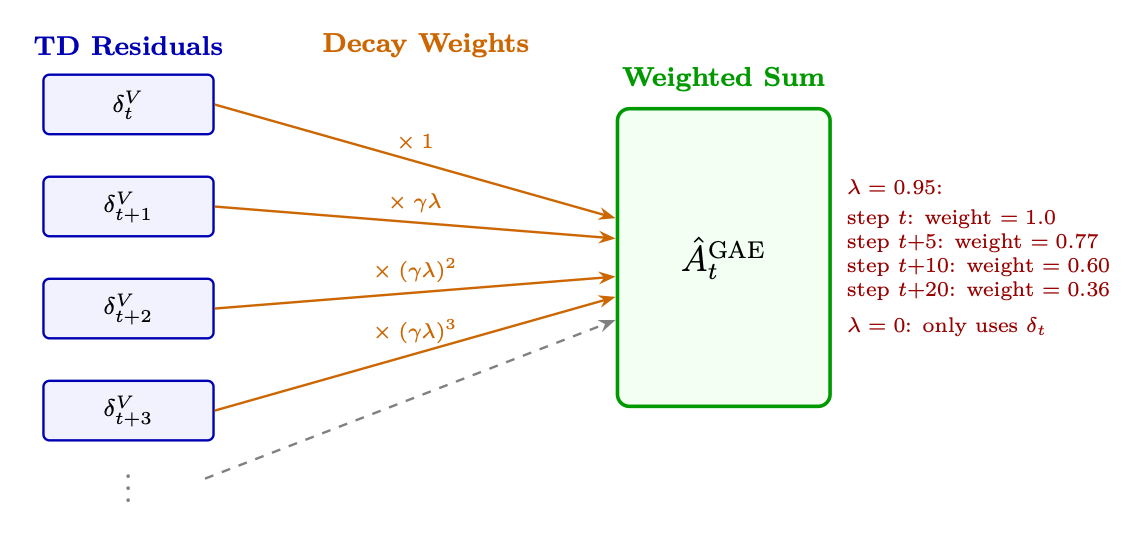
\includegraphics[width=0.85\textwidth]{figures/fig_022_fig22.png}
% \caption{GAE data flow: each TD residual $\delta_{t+l}^V$ is weighted by $(\gamma\lambda)^l$ before summation. Higher $\lambda$ includes more future residuals (lower bias, higher variance).}
\caption{GAE 数据流：每个 TD 残差 $\delta_{t+l}^V$ 在求和前被乘以权重 $(\gamma\lambda)^l$。$\lambda$ 越大，纳入的未来残差越多（偏差更低，方差更高）。}
\end{figure}

% \begin{intuitionbox}[What $\lambda$ Controls --- Bias-Variance Tradeoff]
\begin{intuitionbox}[$\lambda$ 控制什么——偏差-方差权衡]
\begin{itemize}
  % \item $\lambda = 0$: $\hat{A}_t = \delta_t = r_t + \gamma V(s_{t+1}) - V(s_t)$. Trust value function completely. Low variance, but biased if $V$ is inaccurate.
  \item $\lambda = 0$：$\hat{A}_t = \delta_t = r_t + \gamma V(s_{t+1}) - V(s_t)$。完全信任价值函数。方差低，但若 $V$ 不准确则有偏。
  % \item $\lambda = 1$: $\hat{A}_t = \sum_l \gamma^l r_{t+l} - V(s_t)$. Full Monte Carlo return minus baseline. Unbiased but very high variance.
  \item $\lambda = 1$：$\hat{A}_t = \sum_l \gamma^l r_{t+l} - V(s_t)$。完整 Monte Carlo 回报减去基线。无偏但方差极高。
  % \item $\lambda = 0.95$ (standard): Sweet spot. Mostly trusts $V$ but corrects with actual returns for distant effects. Works because value head becomes accurate after initial training.
  \item $\lambda = 0.95$（标准取值）：黄金平衡点。主要信任 $V$，但在远期效应上用实际回报修正。之所以可行，是因为价值头在初始训练后会变得准确。
\end{itemize}

% For LLMs specifically: $\gamma = 1.0$ (no time discounting --- all tokens matter equally in single-turn), $\lambda = 0.95$.
针对 LLM 的常用取值：$\gamma = 1.0$（无时间折扣——单轮对话中所有 token 权重相等），$\lambda = 0.95$。
\end{intuitionbox}

% \subsection{Intuitive Mapping of Bias and Variance in GAE}
\subsection{GAE 中偏差与方差的直观映射}
\label{intuitive-mapping-of-bias-and-variance-in-gae}

% In supervised learning, bias and variance stem from structural model assumptions. In reinforcement learning via GAE, they stem from \textbf{how much you trust a flawed model versus how much you trust a chaotic environment}:
在监督学习中，偏差与方差源于模型的结构性假设。而在通过 GAE 进行的强化学习中，它们源于\textbf{你信任有缺陷的模型有多深 vs 你信任混乱的环境有多深}：

\begin{itemize}
  % \item \textbf{Bias (Systemic Misalignment):} Arises when the estimator relies on the structural assumptions and imperfect predictions of the value network $V_\theta$. If $\theta$ is under-trained or lacks capacity, the baseline guesses are systematically wrong.
  \item \textbf{偏差（系统性偏离）}：当估计器依赖于价值网络 $V_\theta$ 的结构性假设与不完美预测时产生。如果 $\theta$ 训练不足或容量不够，基线猜测就会系统性出错。
  % \item \textbf{Variance (Sample Jitteriness):} Arises when the estimator relies on long, unconstrained environmental trajectories. Stochastic transitions, random seeds, and policy execution noise accumulate over long horizons, causing empirical sample rewards to swing wildly between rollouts.
  \item \textbf{方差（样本抖动）}：当估计器依赖于长且无约束的环境轨迹时产生。随机转移、随机种子与策略执行噪声在长时间步上累积，导致不同 rollout 之间的实际样本奖励剧烈波动。
\end{itemize}

% \subsection{The Architectural Spectrum: Boundary Analysis}
\subsection{架构光谱：边界情形分析}
\label{the-architectural-spectrum-boundary-analysis}

\begin{figure}[ht!]
\centering
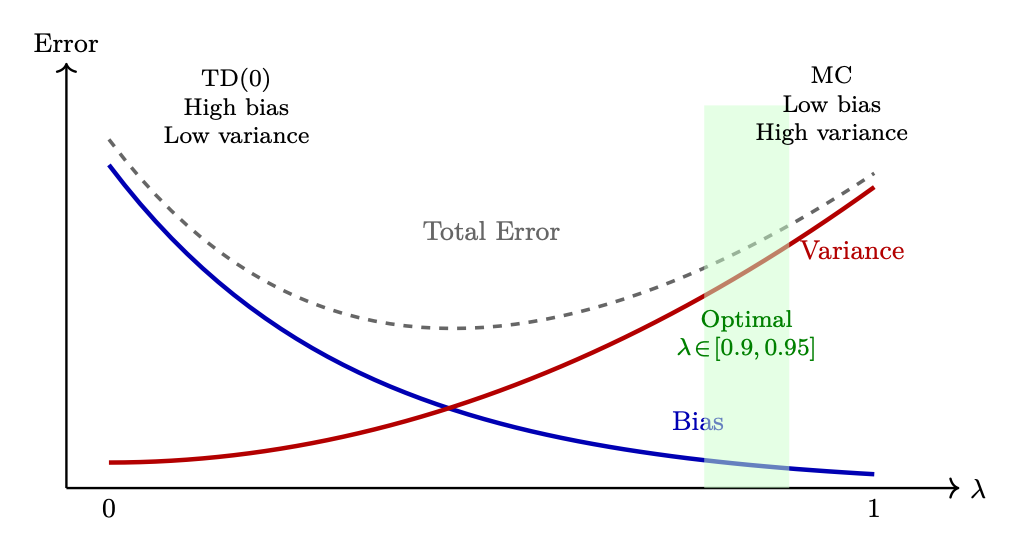
\includegraphics[width=0.85\textwidth]{figures/fig_023_fig23.png}
% \caption{Bias vs. Variance in GAE: $\lambda$ controls the trade-off. Small $\lambda$ (left) yields high bias / low variance via bootstrapping; large $\lambda$ (right) yields low bias / high variance using full Monte Carlo returns. The optimal choice ($\lambda \in [0.9, 0.95]$) balances stable training with accurate long-horizon credit assignment.}
\caption{GAE 中的偏差 vs 方差：$\lambda$ 控制这一权衡。较小的 $\lambda$（左）通过自举得到高偏差/低方差；较大的 $\lambda$（右）使用完整 Monte Carlo 回报得到低偏差/高方差。最优选择（$\lambda \in [0.9, 0.95]$）在稳定训练与准确的长程信用分配之间取得平衡。}
\end{figure}

% The hyperparameter $\lambda$ serves as a slide-rule between two fundamental estimation paradigms.
超参数 $\lambda$ 充当了两种基本估计范式之间的「滑尺」。

% \begin{keybox}[High Bias / Low Variance Limit ($\lambda = 0$)]
\begin{keybox}[高偏差/低方差的限制（$\lambda = 0$）]
\begin{equation}
\hat{A}_t^{\text{GAE}(\gamma, 0)} = \delta_t^V = r_t + \gamma V_\theta(s_{t+1}) - V_\theta(s_t)
\end{equation}

\begin{itemize}
  % \item \textbf{Behavior}: The advantage is heavily dictated by the current state of parameters $\theta$.
  \item \textbf{行为}：优势在很大程度上由参数 $\theta$ 的当前状态决定。
  % \item \textbf{Intuition}: Highly \textbf{biased} because the network is grading its own performance over a 1-step window; if $V_\theta$ is inaccurate, the gradient step is corrupted. Low \textbf{variance} because it ignores future stochastic events beyond step $t+1$, leading to smooth, stable parameter updates.
  \item \textbf{直觉}：高度\textbf{有偏}，因为网络在 1 步窗口内为自己打分；若 $V_\theta$ 不准确，梯度步就会被破坏。\textbf{方差低}，因为它忽略 $t+1$ 步之后的未来随机事件，从而产生平滑、稳定的参数更新。
  % \item \textbf{Risk}: Policy traps in sub-optimal local minima --- never discovers complex delayed reward sequences.
  \item \textbf{风险}：策略陷入次优局部极小——永远发现不了复杂的延迟奖励序列。
\end{itemize}
\end{keybox}

% \begin{keybox}[Low Bias / High Variance Limit ($\lambda = 1$)]
\begin{keybox}[低偏差/高方差的限制（$\lambda = 1$）]
% When $\lambda = 1$, intermediate value terms telescopically cancel, reducing GAE to Monte Carlo return minus baseline:
当 $\lambda = 1$ 时，中间的价值项相互裂项相消，GAE 退化为 Monte Carlo 回报减去基线：
\begin{equation}
\hat{A}_t^{\text{GAE}(\gamma, 1)} = \sum_{l=0}^{\infty} \gamma^l r_{t+l} - V_\theta(s_t)
\end{equation}

\begin{itemize}
  % \item \textbf{Behavior}: Discards bootstrap look-aheads and sums up the literal reality of the entire episode.
  \item \textbf{行为}：舍弃自举式前瞻，将整个 episode 的实际现实进行累加。
  % \item \textbf{Intuition}: Completely \textbf{unbiased} with respect to true environment dynamics --- measures actual rewards instead of neural approximations. However, exhibits extreme \textbf{variance}: minor perturbations early in an episode can result in completely divergent total returns, causing policy updates to become erratic.
  \item \textbf{直觉}：对真实的环境转移完全\textbf{无偏}——衡量的是实际奖励而非神经网络近似。然而表现出极端的\textbf{高方差}：episode 早期的微小扰动可能导致完全不同的总回报，使策略更新变得不稳定。
  % \item \textbf{Risk}: Destructive gradient updates; training explosions.
  \item \textbf{风险}：破坏性梯度更新；训练爆炸。
\end{itemize}
\end{keybox}

% \subsection{The Trade-off Matrix}
\subsection{权衡矩阵}
\label{the-trade-off-matrix}

% By selecting $\lambda \in [0.95, 0.99]$, GAE minimizes the total mean squared error of the advantage estimate:
通过选择 $\lambda \in [0.95, 0.99]$，GAE 可以最小化优势估计的总均方误差：

\begin{table}[ht!]
\centering\small
% \caption{Operational comparison of GAE parameter choices.}
\caption{GAE 参数选择的操作性对比。}
\noindent\begin{tabularx}{\linewidth}{@{}l Z{0.78} Z{0.88} Z{1.34}@{}}
\toprule
% \textbf{Configuration} & \textbf{Statistical Properties} & \textbf{Core Reliance} & \textbf{Practical Risk} \\
\textbf{配置} & \textbf{统计特性} & \textbf{核心依赖} & \textbf{实际风险} \\
\midrule
% $\lambda = 0$ & High Bias, Low Variance & Model parameters ($\theta$) & Policy traps in sub-optimal local minima \\
$\lambda = 0$ & 高偏差、低方差 & 模型参数（$\theta$） & 策略陷入次优局部极小 \\
% $\lambda \in [0.95, 0.99]$ & Balanced (Optimal MSE) & Hybrid blending & Requires tuning based on environment stochasticity \\
$\lambda \in [0.95, 0.99]$ & 均衡（最优 MSE） & 混合融合 & 需要根据环境随机性进行调参 \\
% $\lambda = 1$ & Low Bias, High Variance & Empirical environment rollout & Destructive gradient updates; training explosion \\
$\lambda = 1$ & 低偏差、高方差 & 经验性环境 rollout & 破坏性梯度更新；训练爆炸 \\
\bottomrule
\end{tabularx}
\end{table}

% \subsection{\texorpdfstring{Diagnostics for Tuning $\lambda$}{Diagnostics for Tuning lambda}}
\subsection{\texorpdfstring{$\lambda$ 调参诊断}{lambda 调参诊断}}
\label{diagnostics-for-tuning-lambda}

% Monitoring training curves yields direct insight into whether bias or variance dominates:
监控训练曲线能直接揭示当前主导因素是偏差还是方差：

\begin{enumerate}
  % \item \textbf{High Variance Indicators}: Policy entropy drops precipitously while explained variance of the value function becomes highly negative or erratic $\rightarrow$ policy updates are noisy. \textbf{Remedy}: Lower $\lambda$ to smooth target updates.
  \item \textbf{高方差指标}：策略熵骤降，同时价值函数的解释方差变得高度为负或剧烈波动 $\rightarrow$ 策略更新噪声大。\textbf{对策}：降低 $\lambda$ 以平滑目标更新。
  % \item \textbf{High Bias Indicators}: Agent achieves early stable training but completely fails to discover complex delayed reward sequences $\rightarrow$ under-estimating long-horizon dependencies due to bootstrapping. \textbf{Remedy}: Raise $\lambda$ closer to $1.0$ to expose policy to real downstream trajectory signals.
  \item \textbf{高偏差指标}：智能体在早期获得稳定训练，但完全无法发现复杂的延迟奖励序列 $\rightarrow$ 由于自举导致对长程依赖的低估。\textbf{对策}：将 $\lambda$ 提高至接近 $1.0$，让策略接触真实的下游轨迹信号。
\end{enumerate}

% \section{On-Policy vs Off-Policy --- Detailed Comparison}
\section{同策略 vs 异策略——详细对比}
\label{on-policy-vs-off-policy-detailed-comparison}

\begin{center}
\begin{tabular}{@{}l l l@{}}
\toprule
 & \textbf{On-Policy} & \textbf{Off-Policy} \\
\midrule
% \textbf{Data source} & Current policy $\pi_\theta$ only & Any policy (replay buffer) \\
\textbf{数据来源} & 仅当前策略 $\pi_\theta$ & 任意策略（重放缓冲区） \\
% \textbf{After update} & Old data is invalid, must regenerate & Old data still usable \\
\textbf{更新之后} & 旧数据失效，必须重新生成 & 旧数据仍可使用 \\
% \textbf{Sample efficiency} & Low (data used once) & High (data reused many times) \\
\textbf{样本效率} & 低（数据仅用一次） & 高（数据可多次复用） \\
% \textbf{Stability} & More stable (consistent distribution) & Can diverge (distribution mismatch) \\
\textbf{稳定性} & 更稳定（分布一致） & 可能发散（分布不匹配） \\
% \textbf{Examples} & REINFORCE, PPO, A2C, GRPO & Q-Learning, DQN, SAC, DPO \\
\textbf{示例} & REINFORCE、PPO、A2C、GRPO & Q-Learning、DQN、SAC、DPO \\
% \textbf{For LLMs} & PPO, GRPO (generate fresh each step) & DPO (static preference dataset) \\
\textbf{用于 LLM} & PPO、GRPO（每步重新生成） & DPO（静态偏好数据集） \\
\bottomrule
\end{tabular}
\end{center}

% \begin{intuitionbox}[On/Off-Policy for RLHF Methods]
\begin{intuitionbox}[RLHF 方法的同/异策略属性]
% \textbf{PPO/GRPO are on-policy}: Generate responses with current policy, compute advantages, update, discard data, generate again. This is why generation is 60\% of compute --- you regenerate every step.
\textbf{PPO/GRPO 是同策略}：用当前策略生成回复，计算优势，更新，丢弃数据，再次生成。这就是为何生成占据 60\% 算力——每一步都要重新生成。

% \textbf{DPO is off-policy}: Train on a fixed preference dataset. No generation during training. Much cheaper but suffers from distribution shift (data becomes stale as policy changes).
\textbf{DPO 是异策略}：在固定的偏好数据集上训练。训练过程中无需生成。便宜得多，但会遭受分布偏移问题（随策略变化数据逐渐过时）。

% \textbf{Online DPO is a hybrid}: Generates fresh data (on-policy generation) but uses DPO's supervised loss (off-policy-style optimization). Gets benefits of both.
\textbf{在线 DPO 是混合体}：生成新鲜数据（同策略生成），但使用 DPO 的监督损失（异策略式优化）。兼具两者优势。

% \textbf{PPO's cleverness}: Uses the clip ratio $r = \pi_\text{new}/\pi_\text{old}$ to squeeze multiple gradient steps from one batch of on-policy data (4 epochs), making it ``slightly off-policy'' in a controlled way.
\textbf{PPO 的巧妙之处}：使用裁剪比率 $r = \pi_\text{new}/\pi_\text{old}$，从同一批同策略数据中榨取多步梯度更新（通常 4 个 epoch），以可控方式使其变得「略带异策略」。
\end{intuitionbox}

% \section{Model-Based vs Model-Free}
\section{基于模型 vs 无模型}
\label{model-based-vs-model-free}

\begin{center}
\begin{tabular}{@{}l l l@{}}
\toprule
 & \textbf{Model-Free} & \textbf{Model-Based} \\
\midrule
% \textbf{What's learned} & Policy $\pi$ and/or value $V$/$Q$ directly & Environment model $\hat{P}(s'|s,a)$ \\
\textbf{所学内容} & 直接学习策略 $\pi$ 和/或价值 $V$/$Q$ & 环境模型 $\hat{P}(s'|s,a)$ \\
% \textbf{Planning} & No planning, reactive decisions & Can simulate future trajectories \\
\textbf{规划能力} & 无规划，反应式决策 & 可以模拟未来轨迹 \\
% \textbf{Sample efficiency} & Low (must experience everything) & High (can plan in imagination) \\
\textbf{样本效率} & 低（必须经历所有情况） & 高（可在想象中规划） \\
% \textbf{Accuracy} & No model bias & Model errors compound \\
\textbf{准确性} & 无模型偏差 & 模型误差会累积 \\
% \textbf{When to use} & Complex/unknown dynamics & Simple dynamics, need efficiency \\
\textbf{何时使用} & 复杂/未知的转移 & 简单转移，追求效率 \\
% \textbf{Examples} & PPO, DQN, SAC~\cite{haarnoja2018soft} & MuZero~\cite{schrittwieser2020mastering}, Dreamer~\cite{hafner2020dream}, AlphaGo~\cite{silver2016mastering} \\
\textbf{示例} & PPO、DQN、SAC~\cite{haarnoja2018soft} & MuZero~\cite{schrittwieser2020mastering}、Dreamer~\cite{hafner2020dream}、AlphaGo~\cite{silver2016mastering} \\
\bottomrule
\end{tabular}
\end{center}

% \begin{intuitionbox}[Why LLM RL is Model-Free]
\begin{intuitionbox}[为什么 LLM RL 是无模型的]
% Language generation dynamics are trivial (append token to sequence --- deterministic transitions). The ``model'' of the environment is not the bottleneck. What's hard is the \textbf{reward} --- predicting what humans will prefer. This makes model-based methods unnecessary for LLM RL.
语言生成的状态转移是平凡的（将 token 追加到序列——确定性转移）。环境「模型」并非瓶颈。难的是\textbf{奖励}——预测人类的偏好。这使得 model-based 方法对 LLM RL 来说没有必要。

% The reward model in RLHF could be seen as a ``model'' in some sense (it predicts human preference), but it's used as a reward signal, not for planning/simulation. LLM RL is fundamentally model-free policy optimization.
RLHF 中的奖励模型在某种意义上也可以被看作一种「模型」（它预测人类偏好），但它被用作奖励信号，而非用于规划/模拟。LLM RL 本质上是无模型的策略优化。
\end{intuitionbox}

% \section{Reward Shaping}
\section{奖励塑形（Reward Shaping）}
\label{reward-shaping}

% \textbf{Reward shaping}~\cite{ng1999policy} is a technique where a developer modifies or supplements the environment's original reward function. Its primary objective is to transform a \textbf{sparse reward} scenario --- where the agent receives feedback only upon final task completion --- into a \textbf{dense reward} scenario with intermediate feedback signals to accelerate convergence.
\textbf{奖励塑形（Reward Shaping）}~\cite{ng1999policy}是一种由开发者修改或补充环境原始奖励函数的技术。其主要目的是将\textbf{稀疏奖励}场景（智能体仅在任务最终完成时才获得反馈）转换为带有中间反馈信号的\textbf{稠密奖励}场景，以加速收敛。

% \subsection{The Mathematical Framework}
\subsection{数学框架}
\label{the-mathematical-framework}

% Let the original reward at time step $t$ be $R_t(s, a, s')$. The reshaped reward adds an auxiliary shaping function $F$:
设时间步 $t$ 的原始奖励为 $R_t(s, a, s')$。重塑后的奖励添加了一个辅助塑形函数 $F$：
\begin{equation}
\boxed{R'_t(s, a, s') = R_t(s, a, s') + F(s, a, s')}
\end{equation}

% \begin{warningbox}[The Risk of Naive Reshaping: Reward Hacking]
\begin{warningbox}[朴素塑形的风险：奖励黑客（Reward Hacking）]
% If $F(s, a, s')$ is arbitrarily designed, the agent will find structural loopholes to maximize auxiliary signals while ignoring the global objective.
如果 $F(s, a, s')$ 被随意设计，智能体会找到结构性漏洞来最大化辅助信号，同时忽略全局目标。

% \textbf{Example}: A navigation agent rewarded for reaching intermediate landmarks might learn to loop indefinitely around a single checkpoint to accumulate infinite rewards --- without ever reaching the destination.
\textbf{示例}：一个因到达中间地标而获得奖励的导航智能体可能学会无限绕着某个检查点循环以累积无限奖励——而永远不会到达目的地。

% In LLMs: a model rewarded for ``sounding confident'' might learn to always start with ``Absolutely!'' regardless of accuracy.
在 LLM 中：若模型因「听起来自信」而获得奖励，它可能学会无论准确与否都以「Absolutely!」开头。
\end{warningbox}

% \subsection{Potential-Based Reward Shaping (PBRS)}
\subsection{基于势函数的奖励塑形（Potential-Based Reward Shaping，PBRS）}
\label{potential-based-reward-shaping-pbrs}

% To mathematically guarantee that reshaping does \textbf{not} alter the optimal policy, use \textbf{Potential-Based Reward Shaping}. The shaping function $F$ is constrained to the difference in a scalar potential function $\Phi$ across states:
为了从数学上保证塑形\textbf{不会}改变最优策略，可使用\textbf{基于势函数的奖励塑形（PBRS）}。塑形函数 $F$ 被约束为跨状态的标量势函数 $\Phi$ 之差：
\begin{equation}
\boxed{F(s, a, s') = \gamma\, \Phi(s') - \Phi(s)}
\end{equation}

% where $\Phi: \mathcal{S} \to \mathbb{R}$ is a real-valued potential function evaluating the desirable proximity of a state to the goal, and $\gamma$ is the discount factor.
其中 $\Phi: \mathcal{S} \to \mathbb{R}$ 是一个实值势函数，衡量某状态相对目标的接近程度，$\gamma$ 是折扣因子。

% The complete PBRS reward:
完整的 PBRS 奖励：
\begin{equation}
R'(s, a, s') = R(s, a, s') + \gamma\, \Phi(s') - \Phi(s)
\end{equation}

% \subsection{Theoretical Guarantees}
\subsection{理论保证}
\label{theoretical-guarantees}

% \begin{keybox}[PBRS Policy Invariance Theorem]
\begin{keybox}[PBRS 策略不变性定理]
\begin{itemize}
  % \item \textbf{Policy Invariance}: The optimal policy $\pi^*$ under the reshaped reward $R'$ is \textbf{identical} to the optimal policy under the original reward $R$. The shaping cannot introduce sub-optimal behaviors.
  \item \textbf{策略不变性}：在重塑奖励 $R'$ 下的最优策略 $\pi^*$ 与原始奖励 $R$ 下的最优策略\textbf{完全相同}。塑形不会引入次优行为。
  % \item \textbf{Loop Immunity}: Any cyclic trajectory starting and ending at the same state results in net potential change of exactly zero ($\Phi(s) - \Phi(s) = 0$). The agent cannot exploit loops to hack the reward.
  \item \textbf{回路免疫}：任何从某状态出发又回到同一状态的循环轨迹，其净势能变化恰好为零（$\Phi(s) - \Phi(s) = 0$）。智能体无法利用回路来作弊式刷奖励。
  % \item \textbf{Convergence Acceleration}: While the optimal policy is unchanged, the shaped reward provides denser gradient signals, enabling the agent to converge 5--50$\times$ faster in sparse reward environments.
  \item \textbf{收敛加速}：尽管最优策略不变，塑形后的奖励提供了更稠密的梯度信号，使智能体在稀疏奖励环境下收敛速度提升 5--50 倍。
\end{itemize}
\end{keybox}
